%!TEX root = Manuscrit.tex
\chapter{État de l'art}
\label{chap:etat}
\citationChap{An algorithm must be seen to be believed.}{Donald Knuth}
\minitoc

\chapsummary{%
	\lettrine{C}{e} chapitre introduit les bases théoriques en apprentissage profond sur lesquelles s'appuie la suite du manuscrit. Dans un premier temps, nous rappelons brièvement les motivations et les grandes étapes de construction des réseaux de neurones artificiels modernes avant de détailler le fonctionnement des réseaux convolutifs profonds. Dans un second temps, nous étudierons plus en détail les applications de ces réseaux en vision par ordinateur et notamment pour la segmentation sémantique. Enfin, nous présenterons un tour d'horizon des méthodes classiques d'interprétation d'images de télédétection en nous concentrant sur les approches d'apprentissage et les spécificités liées à l'observation de la Terre.
}
\newpage

\begin{figure}[h]
  \begin{subfigure}{0.5\textwidth}
     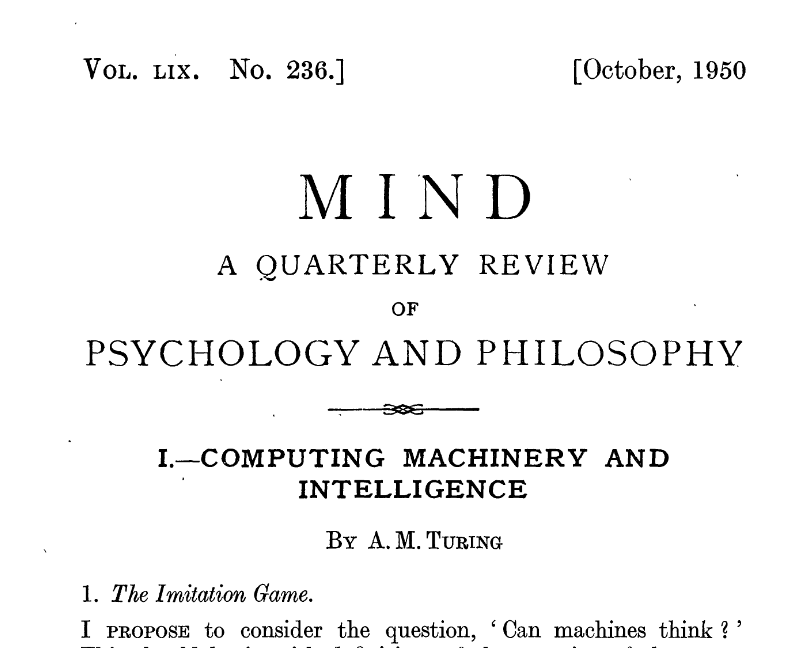
\includegraphics[width=\textwidth]{turing}
     %\label{fig:turing}
  \end{subfigure}
  \begin{subfigure}{0.5\textwidth}
     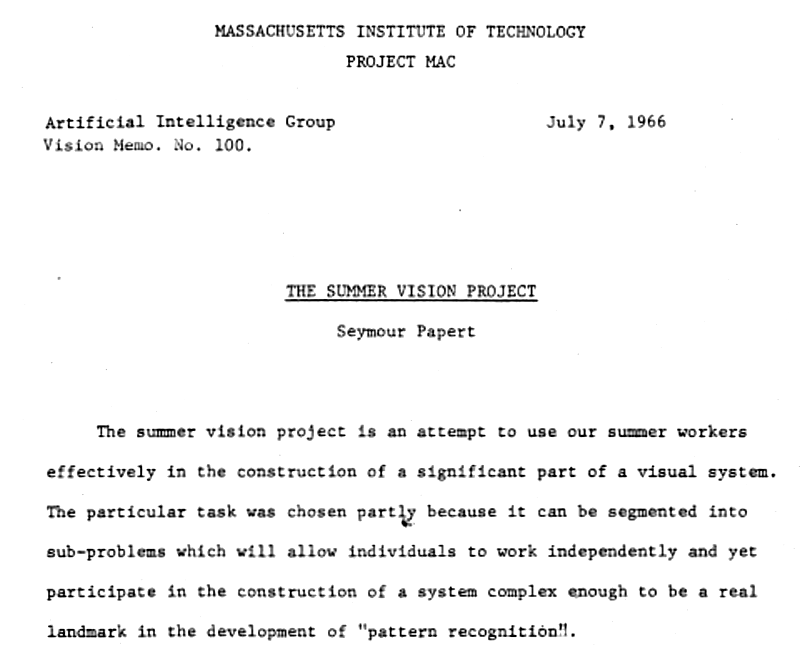
\includegraphics[width=\textwidth]{summer_vision}
     %\label{fig:summer_vision}
  \end{subfigure}
  \caption[Introductions de \emph{Computing Machinery and Intelligence} (Turing, 1950) et \emph{Summer Vision Project} (Papert, 1966).]{Introductions de~\citet{turing_computing_1950} et~\citet{papert_summer_1966}, deux documents fondateurs de l'intelligence artificielle et de la vision par ordinateur.}
  \label{fig:introductions}
\end{figure}

Cette thèse repose sur de nombreux travaux antérieurs en vision par ordinateur, intelligence artificielle et observation de la Terre. Dans ce chapitre, nous allons mettre en place le cadre scientifique fondamental sur lequel nous nous appuierons par la suite. Dans un premier temps, nous allons exposer les principes de l'apprentissage profond et formaliserons la théorie des réseaux de neurones artificiels convolutifs. Dans un second temps, nous détaillerons les applications de ces modèles d'apprentissage pour l'interprétation d'images, sous la forme d'une tâche dite de segmentation sémantique. Enfin, nous discuterons des études récentes sur l'interprétation automatisée d'images de télédétection, ce qui nous permettra d'identifier les spécificités applicatives liées à l'observation de la Terre.

\section{Apprentissage profond pour la vision artificielle}

\subsection{Historique de l'apprentissage profond}

La possibilité d'attribuer des capacités cognitives à un ordinateur est formalisée pour la première fois par Alan \textsc{Turing} en 1950~\cite{turing_computing_1950} (cf.~\cref{fig:introductions}). Dans \og \emph{Computing Machinery and Intelligence} \fg, Turing s'intéresse au cadre formel qui permettrait de répondre à la question suivante: \og{} une machine peut-elle penser ? \fg{}. Selon lui, un ordinateur intelligent serait défini par sa capacité à imiter un humain, de manière à ce que d'autres individus soient incapables de discerner sa véritable nature. Toutefois, Turing ne répond pas à la question du \og comment \fg{} et ne propose pas de solution à ce défi.

Pourtant, en 1943, Warren \textsc{McCulloch} et Walter \textsc{Pitts} proposaient déjà un système de neurones artificiels booléens~\cite{mcculloch_logical_1943} dotés de deux états\,: actif ou inactif. Ils définissent formellement un neurone comme étant un automate fini muni d'une fonction de transfert, permettant de transformer un ensemble d'entrées en une valeur de sortie. Certains neurones ne recevaient aucun signal d'un autre neurone, mais constituaient eux-mêmes le signal d'entrée. Les autres neurones calculaient alors des combinaisons logiques à partir des signaux qu'ils recevaient. \citet{mcculloch_logical_1943} montrent que de nombreux prédicats de logique temporelle sont calculables par de tels réseaux booléens. En particulier, une extension de cette théorie réalisée par Stephen \textsc{Kleene} s'intéresse aux réseaux booléens dont le graphe présente des cycles, c'est-à-dire des réseaux \emph{récurrents}. \citet{kleene_representation_1956} prouve notamment que ces réseaux, qui constituent en réalité des automates finis, sont capables de modéliser n'importe quel langage rationnel\footnote{C'est-à-dire un langage défini par une expression régulière.}.

En parallèle, le neuropsychologue Donald \textsc{Hebb} étudie les mécanismes cognitifs d'apprentissage au sein du cerveau. Il théorise ainsi l'apprentissage hebbien, un principe selon lequel la connexion entre deux neurones se renforce à chacune de leurs activations simultanées~\cite{hebb_organization_1949}. De plus, \textsc{Hebb} suggère que certains neurones se regroupent en \og{} assemblées de cellules \fg{} qui s'activent de façon synchronisée, codant ainsi une représentation mentale des signaux envoyés au cerveau. Comme nous allons le voir, ces deux idées constituent des sources d'inspiration considérable pour les stratégies d'apprentissage développés pour l'intelligence artificielle.

En 1957, Frank \textsc{Rosenblatt} définit le perceptron~\cite{rosenblatt_perceptron_1957}. Il s'agit d'un réseau de neurones acyclique, comme ceux de~\citet{mcculloch_logical_1943}. Les entrées et sorties sont booléennes et le réseau ne possède qu'une unique couche. Les poids des connexions sont néanmoins déterminées automatiquement, en utilisant la règle de Hebb~\cite{hebb_organization_1949}.
À la même époque, Bernard \textsc{Widrow} fabrique l'ADALINE~\cite{widrow_adaptive_1960}, une machine à base de memistors s'inspirant elle aussi du modèle de \citeauthor{mcculloch_logical_1943}. L'ADALINE est très proche du perceptron dans sa conception\,: il s'agit d'un réseau linéaire à une couche opérant sur la somme pondérée de ses entrées. Pour déterminer les poids des connexions, \textsc{Widrow} adopte un algorithme de descente de gradient minimisant l'erreur quadratique du modèle.
Cependant, ces deux modèles présentent une lacune majeure. En effet, le perceptron est assuré de pouvoir trouver une frontière séparant les données de manière optimale, mais uniquement si celles-ci sont linéairement séparables. Ces classifieurs étant linéaires, ils ne peuvent pas résoudre de problèmes non-linéairement séparables. Dans le livre \emph{Perceptrons}, \citet{minsky_perceptrons_1969} prouvent qu'un perceptron à une seule couche cachée est incapable de reproduire la fonction XOR quel que soit le nombre de neurones utilisés, et ce en dépit de la simplicité apparente de l'opération. Malheureusement, il n'existe à l'époque aucune stratégie satisfaisante permettant de déterminer les poids optimaux d'un perceptron à plusieurs couches qui présenterait un caractère non-linéaire. Les réseaux de neurones artificiels tombent alors en désuétude pendant plusieurs années.
Dans sa thèse soutenue en 1975~\cite{werbos_beyond_1975}, Paul \textsc{Werbos} formalise un algorithme de descente de gradient pour la minimisation d'erreur dans un réseau de neurones à plusieurs couches en utilisant le théorème de dérivation des fonctions composées. Il nomme cet algorithme \emph{backpropagation} (rétro-propagation). Il faudra toutefois attendre dix ans pour voir apparaître les premières implémentations de l'algorithme de rétro-propagation du gradient pour entraîner des perceptrons multi-couche~\cite{rumelhart_learning_1986,lecun_learning_1986}.\footnote{L'ADALINE sera également adapté en multi-couche avec sa variante MADALINE~\cite{winter_madaline_1988}, utilisant un algorithme spécifique car utilisant la fonction d'activation $\operatorname{signe}$ dont le gradient est nul presque partout. Widrow et Lehr convergent deux ans plus tard vers une structure de Madaline utilisant la fonction sigmoïde comme activation, entraînable par rétropropagation.}

L'étude théorique des réseaux de neurones à propagation avant, et notamment des perceptrons, reprend alors. En 1989, \citet{cybenko_approximation_1989} démontre le théorème d'approximation universelle prouvant que les fonctions calculables par un perceptron sont denses dans l'ensemble des fonctions continues par morceaux, dans le cas de la sigmoïde comme fonction de transfert. \citet{hornik_approximation_1991} généralise ce résultat deux ans plus tard à l'ensemble des fonctions d'activation usuelles. Le théorème formel est rappelé ci-dessous.

\begin{theorem}
Soit $\varphi$ une fonction bornée, croissante non-constante. Soit $C_0^n$ l'ensemble des fonctions continues définies sur $[0,1]^n$. Alors\,:
$$\forall \epsilon > 0, \forall F \in C_0^n, \exists N \in \mathbb{N}^{*}, \text{ des réels } v_i, b_i \in \mathbb{R} \text{ et des vecteurs } \mathbf{w}_i \in \mathbb{R}^n \text{ avec } i \in \{1\dots{}n\} \text{ tels que}$$
$$\hat{F} : \mathbf{x} \rightarrow \sum_{i=1}^N v_i \varphi\left(\mathbf{w}_i^t \mathbf{x} + b_i \right)$$
soit une approximation de $F$ à $\epsilon$ près, c'est-à-dire\,:
$$\forall \mathbf{x} \in [0,1]^n, ~\left| F(\mathbf{x}) - \hat{F}(\mathbf{x}) \right| < \epsilon~.$$
\end{theorem}

Ce résultat signifie que que toute fonction relativement régulière (continue par morceaux sur un ensemble de compacts) peut être approchée avec une précision arbitraire par un perceptron. Il est ainsi prouvé que de tels réseaux de neurones artificiels peuvent simuler presque n'importe quelle fonction, sans pour autant disposer de méthode de construction de tels réseaux. Outre la théorie des perceptrons, leurs applications pratiques dans le cadre de la vision artificielle pour la reconnaissance de formes ont également été étudiées. La reconnaissance de caractères écrits, notamment les chiffres et les lettres, est un problème particulièrement populaire. En 1980, \citet{fukushima_neocognitron_1980} introduit \emph{Neocognitron}, un perceptron multi-couche dont la structure s'inspire des travaux de \citet{hubel_receptive_1959,hubel_receptive_1968} sur les cortex visuels des chats et des singes. Le \emph{Neocognitron} extrait de l'image des caractéristiques locales robustes aux légères déformations, qui sont graduellement combinées en cascade par le réseau. De cette façon, le modèle n'est plus seulement sensible à l'intensité des pixels, mais aux motifs présents dans les variations locales, se rapprochant ainsi du fonctionnement des yeux animaux~\cite{lettvin_what_1959}. En 1989, \citet{lecun_backpropagation_1989} proposent une architecture de perceptron multi-couche pour la reconnaissance de chiffres manuscrits dont la première couche est \emph{convolutive}, entraîné par rétropropagation. Sur ce principe, ils élaborent ensuite l'architecture LeNet-5~\cite{lecun_gradient-based_1998}, premier \glsfirst{CNN} moderne. En 2004, les méthodes de détection et classification d'objets par \gls{CNN} sont évaluées comme étant compétitives, voire supérieure, par rapport aux \gls{SVM} opérant directement sur les pixels. Les premiers travaux utilisant les représentations apprises par les \gls{CNN} pour remplacer les descripteurs images \emph{ad hoc} comme \gls{SIFT}~\cite{lowe_object_1999} ou \gls{HOG}~\cite{dalal_histograms_2005} pour la classification d'objets apparaissent dans les années 2000~\cite{serre_object_2005,huang_large-scale_2006}.

En 2006, \citet{hinton_reducing_2006} introduisent les réseaux de neurones auto-encodeurs capables de compresser un ensemble de données en les projetant dans un espace de dimension plus faible. Leur approche pour la réduction de dimension utilise une pile de \gls{RBM}~\cite{ackley_learning_1985,salakhutdinov_deep_2009}, entraînées successivement couche par couche. Ce modèle hybride est exploré dans un article de 2006~\cite{hinton_fast_2006} qui leur donne le nom de \gls{DBN}. L'année suivante, \citet{bengio_greedy_2007} étendent ce pré-entraînement par couche à des \gls{DBN} pour la régression. Leurs travaux suggèrent notamment que le pré-entraînement permet d'initialiser les couches supérieures à partir de meilleures représentations des abstractions de haut niveau que le hasard. Yoshua \textsc{Bengio} défend par ailleurs l'idée qu'un bon algorithme d'apprentissage doit être capable d'apprendre des représentations sémantiques pertinentes à des niveaux d'abstraction variés à partir de données non nécessairement annotées, c'est-à-dire en apprentissage non supervisé~\cite{bengio_learning_2009}. Il argumente en faveur des modèles profonds comme étant plus expressifs grâce à leur capacité à apprendre des représentations à partir des données, en s'appuyant sur les progrès récents en sciences cognitives concernant le cortex visuel~\cite{serre_quantitative_2007}. L'introduction de fonctions d'activation non-saturantes en 2011~\cite{glorot_deep_2011} permet de s'affranchir du pré-entraînement et des problèmes d'explosion des gradients, qui rendaient jusqu'alors impossible l'entraînement de réseaux très profonds.

C'est également en 2006 que les premières implémentations des \gls{CNN} sur \gls{GPU} voient le jour~\cite{chellapilla_high_2006} pour le traitement automatisé de documents, puis pour l'apprentissage non-supervisé de \gls{DBN}~\cite{raina_large-scale_2009} et la reconnaissance de caractères~\cite{ciresan_deep_2010}. En 2011, Dan \textsc{Cire\c{s}an} propose des méthodes à base de \gls{CNN} qui obtiennent la première place dans deux compétitions\,: reconnaissance de caractères chinois~\cite{liu_icdar_2011} et classification de panneaux de signalisation~\cite{stallkamp_german_2011}. Ces \gls{CNN} obtiennent en outre d'excellents résultats en reconnaissances de caractères latins et en classification d'objets pour des petites images sur la base de données CIFAR-10~\cite{ciresan_multi-column_2012}. En 2010 débute la compétition de reconnaissance d'objets \gls{ILSVRC}, qui utilise comme référence la banque de données ImageNet~\cite{deng_imagenet_2009}. Un million d'images sont annotées pour mille classes d'intérêt différentes. En 2012, la compétition est remportée par \citet*{krizhevsky_imagenet_2012} à l'aide du réseau convolutif profond AlexNet implémenté sur \gls{GPU} à l'aide de la bibliothèque \gls{CUDA}. AlexNet obtient 15\% d'erreur \emph{top-5}\footnote{Une prédiction \emph{top-5} est considérée juste si la classe recherchée fait partie des cinq premières données par le modèle.}, tandis que la seconde méthode du podium n'obtient que 26\%. Ce succès inattendu est à l'origine de l'explosion en popularité des réseaux convolutifs et de l'apprentissage profond dans la communauté de la vision par ordinateur. La compétition \gls{ILSVRC} a été depuis remportée chaque année par les approches \gls{CNN}, aussi bien pour la reconnaissance et la localisation que la segmentation d'objets. Le succès des réseaux convolutifs profonds depuis 2012 est donc dû à la convergence de trois facteurs\,: des avancées théoriques (\gls{ReLU}, réseaux convolutifs) permettant d'entraîner des réseaux plus profonds, la mise à disposition de grandes bases de données annotées pour l'apprentissage supervisé et des implémentations efficaces sur \gls{GPU} rendant les temps de calcul acceptables.

\begin{figure}[t]
  \resizebox{\textwidth}{!}{
  \documentclass{standalone}
\usepackage[utf8]{inputenc}
\usepackage[T1]{fontenc}
\usepackage{tikz}
\begin{document}
  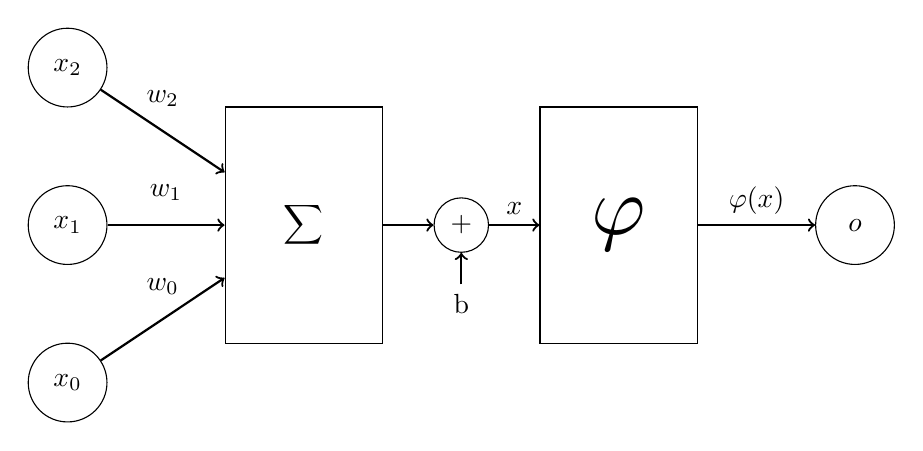
\begin{tikzpicture}

  \node[rectangle, draw=black, minimum size=2cm,minimum height=3cm] (sum) at (3, 0) {$\displaystyle\sum$};

  \foreach\name in {0,1,2}{
      \pgfmathsetmacro\y{2*\name-2}
  	\node[circle, draw=black,minimum size=1cm] (input\name) at (0, \y) {$x_{\name}$};
      \draw[thick,->] (input\name) to node[yshift=5pt,above] {$w_{\name}$} (sum);
  }

  \node[rectangle, draw=black, minimum size=2cm,minimum height=3cm] (phi) at (7, 0) {};
  \node[scale=3] (phisym) at (phi.center) {$\displaystyle\varphi$};

  \node (bias) at (5, -1) {b};
  \node[circle, draw=black] (sumb) at (5, 0) {$+$};
  \draw[thick,->] (sum.east) -- (sumb.west);
  \draw[thick,->] (bias.north) -- (sumb.south);
  \draw[thick,->] (sumb.east) -- node[above] {$x$} (phi.west);
  \node[circle,draw=black,minimum size=1cm] (out) at (10,0) {$o$};
  \draw[thick,->] (phi.east) -- node[above] {$\varphi(x)$} (out.west);
  \end{tikzpicture}
\end{document}


  }
\caption{Modélisation d'un neurone artificiel.}
\label{fig:neurone}
\end{figure}

Dans la suite de cette partie, nous formalisons le cadre théorique des réseaux de neurones artificiels, avant de s'intéresser aux méthodes permettant leur entraînement pour différentes tâches avant de s'intéresser plus particulièrement aux modèles convolutifs.

\subsection{Réseaux de neurones artificiels}

\begin{figure}[t]
  \begin{subfigure}[b]{0.5\textwidth}
    \resizebox{\textwidth}{!}{
    \documentclass{standalone}
\usepackage[utf8]{inputenc}
\usepackage[T1]{fontenc}
\usepackage{tikz}
%%%%%%%%%%%%%%%%%%%%%%%%%%%%%%%%%%%%%%%%
%           Commandes perso            %
%%%%%%%%%%%%%%%%%%%%%%%%%%%%%%%%%%%%%%%%

%% Figures centrées, et en position 'here, top, bottom or page'
\newenvironment{figureth}{%
		\begin{figure}[htbp]
			\centering
	}{
		\end{figure}
		}


%% Tableaux centrés, et en position 'here, top, bottom or page'
\newenvironment{tableth}{%
		\begin{table}[htbp]
			\centering
			%\rowcolors{1}{coleurtableau}{coleurtableau}
	}{
		\end{table}
		}

%% Sous-figures centrées, en position 'top'
\newenvironment{subfigureth}[1]{%
	\begin{subfigure}[t]{#1}
	\centering
}{
	\end{subfigure}
}

\newcommand{\citationChap}[2]{%
	\epigraph{\og \textit{#1} \fg{}}{#2}
}

%% On commence par une page impaire quand on change le style de numérotation de pages
\let\oldpagenumbering\pagenumbering
\renewcommand{\pagenumbering}[1]{%
	\cleardoublepage
	\oldpagenumbering{#1}
}

%% Légende du dataset ISPRS
\newcommand\isprslegende{
Légende\,: \textcolor{Black}{blanc}\,: routes, \textcolor{Blue}{bleu}\,: bâtiments, \textcolor{Cerulean}{cyan}\,: végétation basse, \textcolor{OliveGreen}{vert}\,: arbres, \textcolor{Dandelion}{jaune}\,: véhicules, \textcolor{BrickRed}{rouge}\,: autre.
}

%% Dessiner des réseaux de neurones avec Tikz
\newcommand{\convlayer}[9]{%{h}{w}{d}{name}{color}{x}{y}{z}%{note w}{note h}{note d}
   \def\h{#1}
   \def\w{#2}
   \def\d{#3}
   \def\name{#4}
   \ifthenelse {\equal{#5} {}} {\def\col{white}} {\def\col{#5}}
   \def\x{#6}
   \ifthenelse {\equal{#7} {}} {\def\y{0}} {\def\y{#7}}
   \ifthenelse {\equal{#8} {}} {\def\z{0}} {\def\z{#8}}
   % ne faites pas ça chez vous !
   \ifthenelse {\equal{#9} {}} {\convlayercontinued{}{}{}} {\convlayercontinued#9}
}

\newcommand\convlayercontinued[3]{
   \def\notew{#1}
   \def\noteh{#2}
   \def\noted{#3}
   \coordinate (A) at (\x-\d/2,  \y-\h/2, \z-\w/2);
   \coordinate (B) at (\x-\d/2,  \y-\h/2, \z+\w/2);
   \coordinate (C) at (\x-\d/2,  \y+\h/2, \z+\w/2);
   \coordinate (D) at (\x-\d/2,  \y+\h/2, \z-\w/2);
   \coordinate (E) at (\x+\d/2,  \y-\h/2, \z-\w/2);
   \coordinate (F) at (\x+\d/2,  \y-\h/2, \z+\w/2);
   \coordinate (G) at (\x+\d/2,  \y+\h/2, \z+\w/2);
   \coordinate (H) at (\x+\d/2,  \y+\h/2, \z-\w/2);

    \draw [draw opacity=0.3, fill opacity=0.8, fill=\col!60!white] (A) -- (B) -- (C) -- (D) -- cycle;
    \draw [draw opacity=0.3, fill opacity=0.8, fill=\col!60!white] (A) -- (B) -- (F) -- (E) -- cycle;
    % Face haut
    %\draw [left color=\col!60!white, right color=\col!80!white, shading=axis, shading angle=180] (C) -- (D)  -- (H) -- (G) -- cycle;
    \draw [fill opacity=0.9, fill=\col!70!white] (C) -- node[rotate=45,above] {\small \name} (D) -- (H) -- (G) -- cycle;
    %\draw [fill opacity=0.9, fill=\col!70!white] (C) -- (D) -- node[above] {\small \name} (H) -- (G) -- cycle;
    % Face droite
    \draw [fill opacity=0.9, fill=\col!60!white] (E) -- node[pos=0.75,rotate=45,below] {\scriptsize \notew} (F) -- (G) --  (H) -- cycle;
    % Face avant
    %\draw [shading=axis, left color=\col!60!white, right color=\col!40!white, shading angle=-45] (B) -- node[above,rotate=90] {\scriptsize \noteh} (C) -- (G) -- (F) -- node[below] {\scriptsize \noted}  cycle;
    \draw [fill opacity=0.9, fill=\col!50!white] (B) -- node[above,rotate=90] {\scriptsize \noteh} (C) -- (G) -- (F) -- node[below] {\scriptsize \noted}  cycle;
}

\newcommand{\fclayer}[8]{%{h}{w}{name}{color}{x}{y}{z}
   \def\h{#1}
   \def\w{#2}
   \def\name{#3}
   \ifthenelse {\equal{#4} {}} {\def\col{white}} {\def\col{#4}}
   \def\x{#5}
   \def\y{#6}
   \def\z{#7}
   \def\note{#8}
   \coordinate (A) at (\x-\w/2,  \y-\h/2, \z);
   \coordinate (B) at (\x+\w/2,  \y-\h/2, \z);
   \coordinate (C) at (\x+\w/2,  \y+\h/2, \z);
   \coordinate (D) at (\x-\w/2,  \y+\h/2, \z);

   \pgfmathparse{4*\w}\let\boxwidth\pgfmathresult
    \draw [fill=\col] (A) -- node[below,text width=\boxwidth cm,align=center] {\scriptsize \note} (B) -- (C) -- (D) -- cycle;

    \node (N) at ($(A)!0.5!(B)+(0,-1,0)$) {\name};
}

\newcommand{\alexnet}[4]{%{scale}{x}{y}{z}
  \def\scale{#1}
  \def\alexx{#2}
  \def\alexy{#3}
  \def\alexz{#4}


  \def\coblue{blue!50!white}
  \def\fcgrey{gray!50!white}

  \convlayer{1.3*\scale}{1.3*\scale}{0.02*\scale}{Image}{\coblue}{\alexx}{\alexy}{\alexz}{{227}{227}{3}}
  \convlayer{1.1*\scale}{1.1*\scale}{0.08*\scale}{Conv1}{\coblue}{\alexx+0.7*\scale}{\alexy}{\alexz}{{55}{55}{96}}
  \convlayer{0.7*\scale}{0.7*\scale}{0.5*\scale}{Conv2}{\coblue}{\alexx+1.5*\scale}{\alexy}{\alexz}{{27}{27}{256}}
  \convlayer{0.5*\scale}{0.5*\scale}{0.8*\scale}{Conv3}{\coblue}{\alexx+2.6*\scale}{\alexy}{\alexz}{{13}{13}{384}}
  \convlayer{0.5*\scale}{0.5*\scale}{0.8*\scale}{Conv4}{\coblue}{\alexx+3.8*\scale}{\alexy}{\alexz}{{13}{13}{384}}
  \convlayer{0.5*\scale}{0.5*\scale}{0.5*\scale}{Conv5}{\coblue}{\alexx+4.8*\scale}{\alexy}{\alexz}{{13}{13}{256}}
  \fclayer{\scale}{0.1*\scale}{FC1}{\fcgrey}{\alexx+5.4*\scale}{\alexy}{\alexz}{4096}
  \fclayer{\scale}{0.1*\scale}{FC2}{\fcgrey}{\alexx+5.7*\scale}{\alexy}{\alexz}{4096}
  \fclayer{\scale}{0.1*\scale}{FC3}{\fcgrey}{\alexx+6.0*\scale}{\alexy}{\alexz}{1000}
}

\newcommand{\imagelayer}[7]{%{width}{x}{y}{z}{path}{text_up}{text_down}
    \pgfmathparse{#1}\let\w\pgfmathresult
    \begin{scope}[canvas is yz plane at x=#2]
     \node[transform shape] (source) at (#3, #4) {\includegraphics[angle=-90,width=\w cm]{#5}};
    \end{scope}
     \node [transform shape, rotate=45, above] at (source.east) {#6};
     \node [transform shape, rotate=45, below] at (source.west) {\scriptsize{#7}};
}

\def\fourier{\mathcal{F}}

\newcommand{\lightspectrum}{%
\pgfplotsset{
    % this *defines* a custom colormap ...
    colormap={slategraywhite}{color(0cm)=(red); color(1cm)=(red); color(2cm)=(red); color(3cm)=(red); color(4cm)=(orange); color(5cm)=(yellow); color(6cm)=(green); color(7cm)=(blue); color(8cm)=(blue); color(9cm)=(purple); color(10cm)=(purple); color(12cm)=(black)}
}
\node at (1.5, 2.7) {\small 1mm};
\node at (4, 3) {Infrarouge};
\node at (7.75, 2.7) {\small 800nm};
\node at (9, 3) {Visible};
\node at (10.5, 2.7) {\small 400nm};
\node at (12, 3) {Ultraviolet};
\node at (13.5, 2.7) {\small 10nm};
\draw[->] (1, 2.5) -- (14, 2.5);
\begin{axis}[hide axis,width=16cm,height=4cm,colormap name=slategraywhite]
\addplot[domain=20:1000,samples=1500,ultra thick, point meta=x*x,mesh]{sin(x*x/80)};
\end{axis}
}

% Union généralisée
\newcommand{\wbigcup}{\mathop{\bigcup}\displaylimits}

\newcommand{\res}[2]{#1 {\footnotesize $\pm$ #2}}
\newcommand{\bres}[2]{\textbf{#1} {\footnotesize $\pm$ #2}}
\newcommand{\bbres}[2]{\res{\textit{#1}}{#2}}

\newcommand{\drawkernel}[9]{
\begin{tikzpicture}
	\draw[step=1cm,gray!50!white,very thin] (0,0) grid (3,3);
	\kernelnode{0.5}{0.5}{#1};
	\kernelnode{0.5}{1.5}{#2};
	\kernelnode{0.5}{2.5}{#3};
	\kernelnode{1.5}{0.5}{#4};
	\kernelnode{1.5}{1.5}{#5};
	\kernelnode{1.5}{2.5}{#6};
	\kernelnode{2.5}{0.5}{#7};
	\kernelnode{2.5}{1.5}{#8};
	\kernelnode{2.5}{2.5}{#9};
\end{tikzpicture}
}

\newcommand{\kernelnode}[3]{%{x}{y}{value}
	\ifthenelse{\equal{#3}{0}}{
		\def\kcolor{gray}
	}{
		\def\kcolor{black}
	}
	\node[\kcolor] at (#1, #2) {#3};
}

\newcommand{\chapsummary}[1]{
\section*{Résumé du chapitre :}
\parbox{0.9\linewidth}{
\setlength{\parindent}{4ex}
#1}
}

\newcommand{\eqname}[1]{\tag*{\small (#1)}}

\begin{document}
  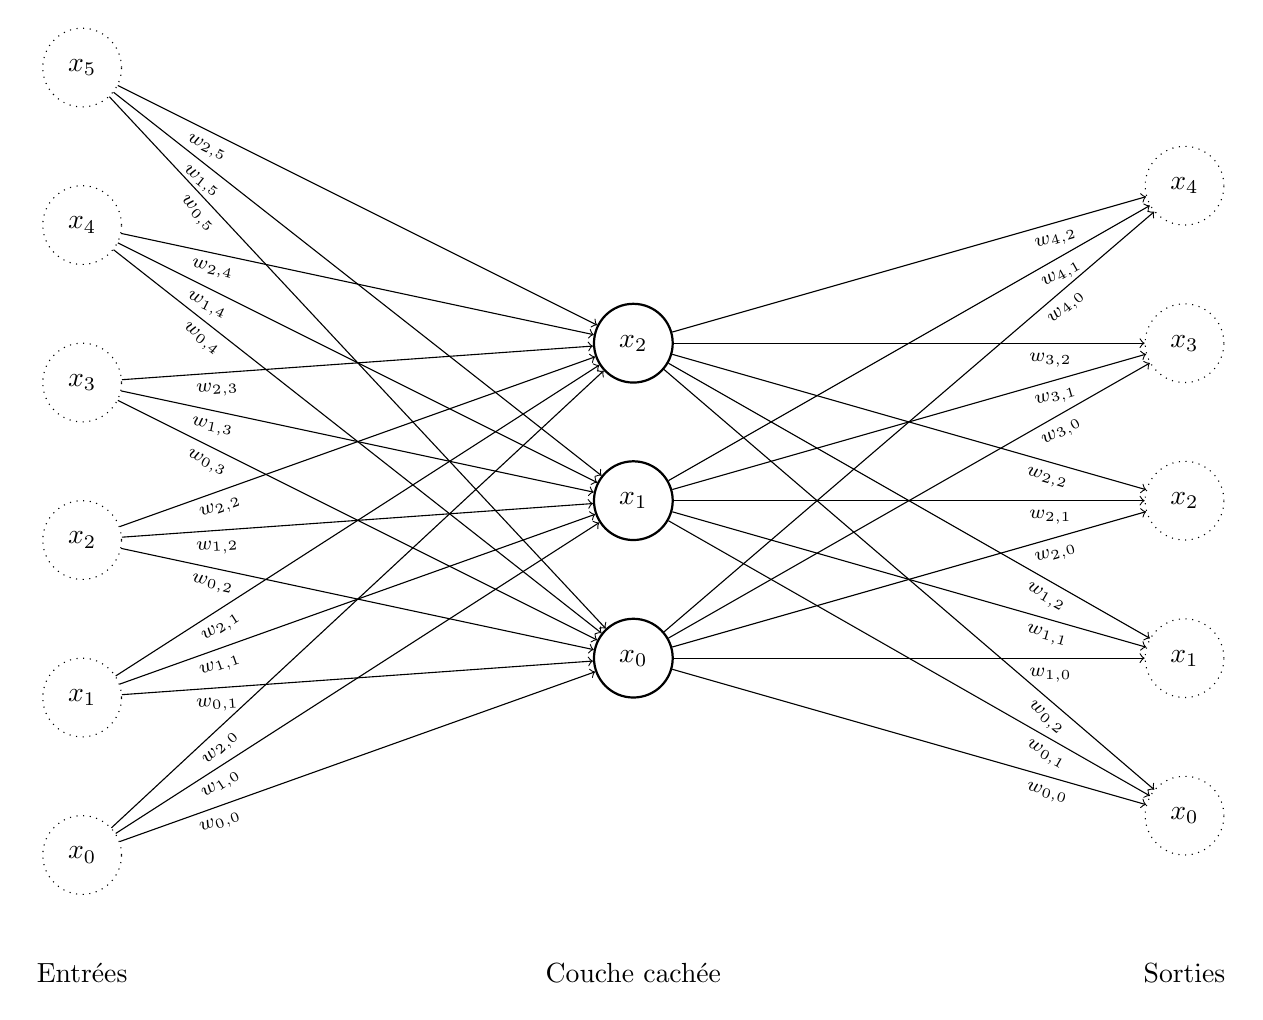
\begin{tikzpicture}
  \foreach\name in {0,1,2,3,4}{
      \pgfmathsetmacro\y{2*\name-3}
  	\node[circle, dotted,draw=black,minimum size=1cm] (output\name) at (7, \y) {$x_{\name}$};
  %    \draw[thick,->] (input\name) to node[yshift=5pt,above] {$w_{\name}$} (sum);
  }

  \foreach\name in {0,1,2}{
      \pgfmathsetmacro\y{2*\name-1}
  	\node[circle, thick,draw=black,minimum size=1cm] (hidden\name) at (0, \y) {$x_{\name}$};
      \foreach\oname in {0,1,2,3,4}{
      \draw[->] (hidden\name) to node[near end, sloped,pos=0.8,below] {\scriptsize $w_{\oname,\name}$} (output\oname);
      }
  }

  \node at (-7, -5) {Entrées};
  \node at (0, -5) {Couche cachée};
  \node at (7, -5) {Sorties};

  \foreach\name in {0,1,2,3,4,5}{
      \pgfmathsetmacro\y{2*\name-3.5}
  	\node[circle, dotted, draw=black,minimum size=1cm] (input\name) at (-7, \y) {$x_{\name}$};
      \foreach\hname in {0,1,2}{
      \draw[->] (input\name) to node[near end, sloped,pos=0.2,below] {\scriptsize $w_{\hname,\name}$} (hidden\hname);
      }
  }
  \end{tikzpicture}
\end{document}

    }
  \caption{Perceptron à une couche cachée.}
  \end{subfigure}%
  \begin{subfigure}[b]{0.5\textwidth}
    \resizebox{\textwidth}{!}{
    \documentclass{standalone}
\usepackage[utf8]{inputenc}
\usepackage[T1]{fontenc}
\usepackage{tikz}
\usepackage{ifthen}
%%%%%%%%%%%%%%%%%%%%%%%%%%%%%%%%%%%%%%%%
%           Commandes perso            %
%%%%%%%%%%%%%%%%%%%%%%%%%%%%%%%%%%%%%%%%

%% Figures centrées, et en position 'here, top, bottom or page'
\newenvironment{figureth}{%
		\begin{figure}[htbp]
			\centering
	}{
		\end{figure}
		}


%% Tableaux centrés, et en position 'here, top, bottom or page'
\newenvironment{tableth}{%
		\begin{table}[htbp]
			\centering
			%\rowcolors{1}{coleurtableau}{coleurtableau}
	}{
		\end{table}
		}

%% Sous-figures centrées, en position 'top'
\newenvironment{subfigureth}[1]{%
	\begin{subfigure}[t]{#1}
	\centering
}{
	\end{subfigure}
}

\newcommand{\citationChap}[2]{%
	\epigraph{\og \textit{#1} \fg{}}{#2}
}

%% On commence par une page impaire quand on change le style de numérotation de pages
\let\oldpagenumbering\pagenumbering
\renewcommand{\pagenumbering}[1]{%
	\cleardoublepage
	\oldpagenumbering{#1}
}

%% Légende du dataset ISPRS
\newcommand\isprslegende{
Légende\,: \textcolor{Black}{blanc}\,: routes, \textcolor{Blue}{bleu}\,: bâtiments, \textcolor{Cerulean}{cyan}\,: végétation basse, \textcolor{OliveGreen}{vert}\,: arbres, \textcolor{Dandelion}{jaune}\,: véhicules, \textcolor{BrickRed}{rouge}\,: autre.
}

%% Dessiner des réseaux de neurones avec Tikz
\newcommand{\convlayer}[9]{%{h}{w}{d}{name}{color}{x}{y}{z}%{note w}{note h}{note d}
   \def\h{#1}
   \def\w{#2}
   \def\d{#3}
   \def\name{#4}
   \ifthenelse {\equal{#5} {}} {\def\col{white}} {\def\col{#5}}
   \def\x{#6}
   \ifthenelse {\equal{#7} {}} {\def\y{0}} {\def\y{#7}}
   \ifthenelse {\equal{#8} {}} {\def\z{0}} {\def\z{#8}}
   % ne faites pas ça chez vous !
   \ifthenelse {\equal{#9} {}} {\convlayercontinued{}{}{}} {\convlayercontinued#9}
}

\newcommand\convlayercontinued[3]{
   \def\notew{#1}
   \def\noteh{#2}
   \def\noted{#3}
   \coordinate (A) at (\x-\d/2,  \y-\h/2, \z-\w/2);
   \coordinate (B) at (\x-\d/2,  \y-\h/2, \z+\w/2);
   \coordinate (C) at (\x-\d/2,  \y+\h/2, \z+\w/2);
   \coordinate (D) at (\x-\d/2,  \y+\h/2, \z-\w/2);
   \coordinate (E) at (\x+\d/2,  \y-\h/2, \z-\w/2);
   \coordinate (F) at (\x+\d/2,  \y-\h/2, \z+\w/2);
   \coordinate (G) at (\x+\d/2,  \y+\h/2, \z+\w/2);
   \coordinate (H) at (\x+\d/2,  \y+\h/2, \z-\w/2);

    \draw [draw opacity=0.3, fill opacity=0.8, fill=\col!60!white] (A) -- (B) -- (C) -- (D) -- cycle;
    \draw [draw opacity=0.3, fill opacity=0.8, fill=\col!60!white] (A) -- (B) -- (F) -- (E) -- cycle;
    % Face haut
    %\draw [left color=\col!60!white, right color=\col!80!white, shading=axis, shading angle=180] (C) -- (D)  -- (H) -- (G) -- cycle;
    \draw [fill opacity=0.9, fill=\col!70!white] (C) -- node[rotate=45,above] {\small \name} (D) -- (H) -- (G) -- cycle;
    %\draw [fill opacity=0.9, fill=\col!70!white] (C) -- (D) -- node[above] {\small \name} (H) -- (G) -- cycle;
    % Face droite
    \draw [fill opacity=0.9, fill=\col!60!white] (E) -- node[pos=0.75,rotate=45,below] {\scriptsize \notew} (F) -- (G) --  (H) -- cycle;
    % Face avant
    %\draw [shading=axis, left color=\col!60!white, right color=\col!40!white, shading angle=-45] (B) -- node[above,rotate=90] {\scriptsize \noteh} (C) -- (G) -- (F) -- node[below] {\scriptsize \noted}  cycle;
    \draw [fill opacity=0.9, fill=\col!50!white] (B) -- node[above,rotate=90] {\scriptsize \noteh} (C) -- (G) -- (F) -- node[below] {\scriptsize \noted}  cycle;
}

\newcommand{\fclayer}[8]{%{h}{w}{name}{color}{x}{y}{z}
   \def\h{#1}
   \def\w{#2}
   \def\name{#3}
   \ifthenelse {\equal{#4} {}} {\def\col{white}} {\def\col{#4}}
   \def\x{#5}
   \def\y{#6}
   \def\z{#7}
   \def\note{#8}
   \coordinate (A) at (\x-\w/2,  \y-\h/2, \z);
   \coordinate (B) at (\x+\w/2,  \y-\h/2, \z);
   \coordinate (C) at (\x+\w/2,  \y+\h/2, \z);
   \coordinate (D) at (\x-\w/2,  \y+\h/2, \z);

   \pgfmathparse{4*\w}\let\boxwidth\pgfmathresult
    \draw [fill=\col] (A) -- node[below,text width=\boxwidth cm,align=center] {\scriptsize \note} (B) -- (C) -- (D) -- cycle;

    \node (N) at ($(A)!0.5!(B)+(0,-1,0)$) {\name};
}

\newcommand{\alexnet}[4]{%{scale}{x}{y}{z}
  \def\scale{#1}
  \def\alexx{#2}
  \def\alexy{#3}
  \def\alexz{#4}


  \def\coblue{blue!50!white}
  \def\fcgrey{gray!50!white}

  \convlayer{1.3*\scale}{1.3*\scale}{0.02*\scale}{Image}{\coblue}{\alexx}{\alexy}{\alexz}{{227}{227}{3}}
  \convlayer{1.1*\scale}{1.1*\scale}{0.08*\scale}{Conv1}{\coblue}{\alexx+0.7*\scale}{\alexy}{\alexz}{{55}{55}{96}}
  \convlayer{0.7*\scale}{0.7*\scale}{0.5*\scale}{Conv2}{\coblue}{\alexx+1.5*\scale}{\alexy}{\alexz}{{27}{27}{256}}
  \convlayer{0.5*\scale}{0.5*\scale}{0.8*\scale}{Conv3}{\coblue}{\alexx+2.6*\scale}{\alexy}{\alexz}{{13}{13}{384}}
  \convlayer{0.5*\scale}{0.5*\scale}{0.8*\scale}{Conv4}{\coblue}{\alexx+3.8*\scale}{\alexy}{\alexz}{{13}{13}{384}}
  \convlayer{0.5*\scale}{0.5*\scale}{0.5*\scale}{Conv5}{\coblue}{\alexx+4.8*\scale}{\alexy}{\alexz}{{13}{13}{256}}
  \fclayer{\scale}{0.1*\scale}{FC1}{\fcgrey}{\alexx+5.4*\scale}{\alexy}{\alexz}{4096}
  \fclayer{\scale}{0.1*\scale}{FC2}{\fcgrey}{\alexx+5.7*\scale}{\alexy}{\alexz}{4096}
  \fclayer{\scale}{0.1*\scale}{FC3}{\fcgrey}{\alexx+6.0*\scale}{\alexy}{\alexz}{1000}
}

\newcommand{\imagelayer}[7]{%{width}{x}{y}{z}{path}{text_up}{text_down}
    \pgfmathparse{#1}\let\w\pgfmathresult
    \begin{scope}[canvas is yz plane at x=#2]
     \node[transform shape] (source) at (#3, #4) {\includegraphics[angle=-90,width=\w cm]{#5}};
    \end{scope}
     \node [transform shape, rotate=45, above] at (source.east) {#6};
     \node [transform shape, rotate=45, below] at (source.west) {\scriptsize{#7}};
}

\def\fourier{\mathcal{F}}

\newcommand{\lightspectrum}{%
\pgfplotsset{
    % this *defines* a custom colormap ...
    colormap={slategraywhite}{color(0cm)=(red); color(1cm)=(red); color(2cm)=(red); color(3cm)=(red); color(4cm)=(orange); color(5cm)=(yellow); color(6cm)=(green); color(7cm)=(blue); color(8cm)=(blue); color(9cm)=(purple); color(10cm)=(purple); color(12cm)=(black)}
}
\node at (1.5, 2.7) {\small 1mm};
\node at (4, 3) {Infrarouge};
\node at (7.75, 2.7) {\small 800nm};
\node at (9, 3) {Visible};
\node at (10.5, 2.7) {\small 400nm};
\node at (12, 3) {Ultraviolet};
\node at (13.5, 2.7) {\small 10nm};
\draw[->] (1, 2.5) -- (14, 2.5);
\begin{axis}[hide axis,width=16cm,height=4cm,colormap name=slategraywhite]
\addplot[domain=20:1000,samples=1500,ultra thick, point meta=x*x,mesh]{sin(x*x/80)};
\end{axis}
}

% Union généralisée
\newcommand{\wbigcup}{\mathop{\bigcup}\displaylimits}

\newcommand{\res}[2]{#1 {\footnotesize $\pm$ #2}}
\newcommand{\bres}[2]{\textbf{#1} {\footnotesize $\pm$ #2}}
\newcommand{\bbres}[2]{\res{\textit{#1}}{#2}}

\newcommand{\drawkernel}[9]{
\begin{tikzpicture}
	\draw[step=1cm,gray!50!white,very thin] (0,0) grid (3,3);
	\kernelnode{0.5}{0.5}{#1};
	\kernelnode{0.5}{1.5}{#2};
	\kernelnode{0.5}{2.5}{#3};
	\kernelnode{1.5}{0.5}{#4};
	\kernelnode{1.5}{1.5}{#5};
	\kernelnode{1.5}{2.5}{#6};
	\kernelnode{2.5}{0.5}{#7};
	\kernelnode{2.5}{1.5}{#8};
	\kernelnode{2.5}{2.5}{#9};
\end{tikzpicture}
}

\newcommand{\kernelnode}[3]{%{x}{y}{value}
	\ifthenelse{\equal{#3}{0}}{
		\def\kcolor{gray}
	}{
		\def\kcolor{black}
	}
	\node[\kcolor] at (#1, #2) {#3};
}

\newcommand{\chapsummary}[1]{
\section*{Résumé du chapitre :}
\parbox{0.9\linewidth}{
\setlength{\parindent}{4ex}
#1}
}

\newcommand{\eqname}[1]{\tag*{\small (#1)}}

\begin{document}

    \begin{tikzpicture}

    \newcommand\drawlayer[7]{%{nombre de neurones}{position en x}{symbole}{nom de la couche}{couche précédente}{n couche précédente}{style}
      \foreach\name in {0,...,#1}{
        \pgfmathsetmacro\y{2*(\name-#1/2)}
      	\node[circle,#7,draw=black,minimum size=1cm] (#4_\name) at (#2, \y) {$#3_{\name}$};
          \ifthenelse{\equal{#5}{}}{}{
		\foreach\oname in {0,...,#6}{
	            {\draw[->] (#5_\oname) to (#4_\name);}
         	 }
      	  }
      }
    }

    \drawlayer{5}{0}{x}{input}{}{}{dotted}
    \drawlayer{3}{4}{h^1}{hidden1}{input}{5}{thick}
    \drawlayer{4}{8}{h^2}{hidden2}{hidden1}{3}{thick}
    \drawlayer{3}{12}{h^3}{hidden3}{hidden2}{4}{thick}
    \drawlayer{3}{16}{y}{output}{hidden3}{3}{dotted}

    \node at (0,-6.5) {Entrées};
    \node at (8,-6.5) {Couches cachées};
    \node at (16,-6.5) {Sorties};

    \end{tikzpicture}

\end{document}


    }
  \caption{Perceptron multi-couche.}
  \end{subfigure}
  \caption{Perceptron à une et plusieurs couches. Les entrées et sorties peuvent être de dimensions variables et sont représentées comme des neurones.}
  \label{fig:perceptron}
\end{figure}

La définition formelle d'un neurone artificiel a été introduite par \textsc{McCulloch} et \textsc{Pitts}~\cite{lettvin_what_1959} en 1959. Un neurone doté d'une fonction de transfert $\varphi$ opère sur un ensemble de $n$ neurones d'entrée émettant chacun une valeur $x_1\dots{}x_n$, auxquels il est connecté par des synapses de poids $w_i$. La valeur d'entrée $x$ du neurone correspond à la somme signaux d'entrée pondérés par les poids de leur synapse. Le neurone émet en sortie l'image $z = \varphi(x)$ de ce signal par sa fonction de transfert. Le schéma de la~\cref{fig:neurone} décrit ce procédé. L'activation en sortie d'un neurone s'obtient donc par la formule
\begin{equation}
z = \varphi\left(\sum_{i=1}^n w_i x_i + b\right)~.
\end{equation}

Plusieurs neurones peuvent être connectés les uns aux autres et forment alors un graphe orienté et pondéré. Un réseau de neurones à propagation avant désigne un graphe neuronal acyclique. En pratique, on considère des graphes $k$-partis que l'on peut alors représenter par \og couches \fg. Dans le cas d'un perceptron à couches multiples, les valeurs des signaux d'entrée et de sortie sont placées dans des couches spécifiques. Les couches de neurones réellement optimisables sont nommées \og couches cachées \fg{} et font l'interface entre l'entrée et la sortie. Les perceptrons multi-couches à une et plusieurs couches cachées sont illustrés dans la~\cref{fig:perceptron}.

La fonction d'activation des neurones peut prendre de nombreuses formes. Il est \emph{a minima} nécessaire que celle-ci soit non-linéaire, sans quoi l'expressivité du réseau se trouve limitée à celle du perceptron, et presque partout différentiable, afin de pouvoir appliquer l'algorithme de rétro-propagation du gradient. La fonction d'activation $\varphi$ est en outre généralement choisie telle que $\varphi$ et sa dérivée $\varphi'$ soient monotones croissantes. La~\cref{fig:saturantes} illustre plusieurs activations communément utilisées dans les réseaux de neurones artificiels profonds\,:
\begin{itemize}
  \item La \textbf{sigmoïde}, ou fonction logistique\,: $\sigma(x) = \frac{1}{1 + e^{-x}}$.
  \item La fonction \textbf{tangente hyperbolique}\,: $\tanh(x) = \frac{1 - e^{-2x}}{1 + e^{-2x}}$.
  \item La \textbf{marche de Heavyside}\,: $H(x) = 0 \text{ si } x < 0 \text{ et } 1 \text{ si } x \geq 0$.
  \item La fonction \textbf{\gls{ReLU}}\,: $ReLU(x) = \max(0,x)$.
\end{itemize}

\begin{figure}[t]
  \begin{subfigure}[b]{0.5\textwidth}
    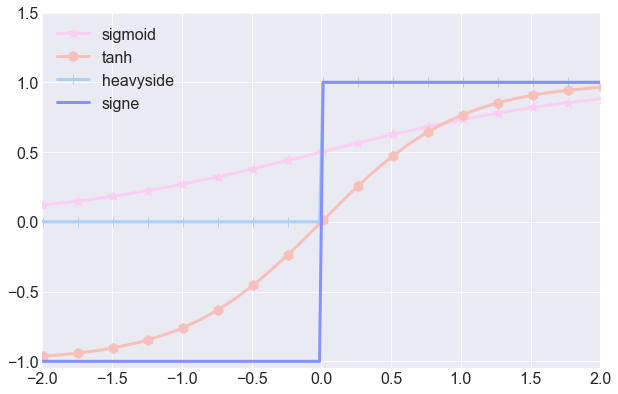
\includegraphics[width=\textwidth]{activations}
    \caption{Fonctions d'activation saturantes.}
    \label{fig:saturantes}
  \end{subfigure}
\begin{subfigure}[b]{0.5\textwidth}
  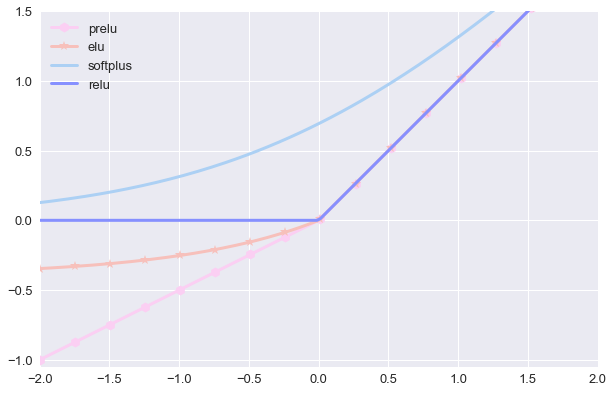
\includegraphics[width=\textwidth]{rectifiers}
  \caption{Fonctions d'activation non-saturantes.}
  \label{fig:rectifiers}
\end{subfigure}
\caption{Exemples de fonctions d'activation.}
\label{fig:activations}
\end{figure}

La marche de Heavyside, tout comme la fonction $\operatorname{signe}$, a des gradients nuls presque partout, sa dérivée étant l'impulsion de Dirac $\delta$. Ceci les rend peu utilisées en pratique car il est impossible de leur appliquer l'algorithme de rétro-propagation du gradient.
La fonction sigmoïde, bien qu'initialement la plus commune, est une fonction saturante qui souffre de gradients évanescents. Ce problème n'est pas circonscrit à la sigmoïde et est particulièrement pregnant dans le cas des réseaux de neurones récurrents~\cite{hochreiter_gradient_2001}. L'accumulation de couches dans le réseau rend géométrique l'évolution des amplitudes du gradient durant la rétro-propagation du gradient. Le produit cumulé de $n$ gradients dans des fonctions d'activation à tendance contractante produit un $n+1$\ieme gradient plus faible que le précédent, et ainsi de suite. À l'inverse, il est possible d'avoir des gradients explosifs dont la norme croît exponentiellement. Ce problème est empiré dans le cas des fonctions saturantes comme la sigmoïde ou la tangente hyperbolique car leurs gradients appartiennent nécessairement à l'intervalle $[0,1]$. L'utilisation de la sigmoïde ou la tangente hyperbolique a varié dans la littérature. \citet{lecun_efficient_1998} recommande d'utiliser la fonction hyperbolique modifiée $f(x) = 1,7159 tanh(\frac{2}{3} x)$, notamment car celle-ci est bornée par $[-1,1]$ et centrée en 0, ce qui est adapté au travail sur des données normalisées à moyenne nulle et variance unitaire.

Désormais, les fonctions d'activation non-linéaires non-saturantes sont majoritairement utilisées dans la littérature afin de limiter les gradients évanescents. En effet, \citet{glorot_deep_2011} ont proposé d'utiliser la fonction \gls{ReLU}, introduite précédemment pour les \gls{DBN}~\cite{nair_rectified_2010}, et la fonction SoftPlus pour n'importe quel type de réseau de neurones. Ils analysent les effets de ces fonctions d'activation sur l'optimisation des réseaux et aboutissent à trois conclusions. Tout d'abord, les fonctions d'activation non-linéaires généralisent dans l'ensemble mieux que les réseaux utilisant $tanh$. Ensuite, les réseaux entraînés avec \gls{ReLU} ne nécessitent pas de pré-apprentissage non-supervisé couche par couche, ce qui accélère grandement les temps d'entraînement. Enfin, ces modèles sont plus parcimonieux que leurs équivalents usuels. Compte-tenu de la simplicité d'implémentation des \gls{ReLU} et leur efficacité calculatoire, ces fonctions ont rapidement été adoptées par la communauté.

Dans l'ensemble, bien que ces hypothèses ne semblent pas nécessaires à la construction de réseaux profonds~\cite{oyallon_building_2017}, la plupart des fonctions d'activation couramment utilisées sont continues, monotones, contractantes et s'appliquent indépendamment sur chaque activation. Plusieurs variantes ont été proposées autour des fonctions linéaires rectifiées, notamment une version paramétrique dont la partie négative est de pente $\alpha > 0$, fixée par l'utilisateur (\emph{Leaky ReLU}~\cite{maas_rectifier_2013}) ou apprenable (\gls{PReLU}~\cite{he_delving_2015}). Une alternative dérivable partout a également été proposée sous la forme de \gls{ELU}~\cite{clevert_fast_2015}.
%Plus récemment, une recherche automatique quasi-exhaustive sur une variété de fonctions d'activation possibles a permis de proposer la \emph{Swish}~\cite{ramachandran_searching_2018} non-linéaire non-saturante mais ayant la particularité d'être non-monotone.
Certaines de ces variantes sont illustrées dans la~\cref{fig:rectifiers} et leur formule est donnée ci-dessous\,:
\begin{itemize}
  \item La fonction \textbf{ReLU}\,: $\operatorname{ReLU}(x) = \max(0,x)$.
  \item La fonction \textbf{SoftPlus}\,: $s^+(x) = \ln(1 + e^x)$.
  \item La fonction \textbf{\emph{Leaky ReLU}}\,: $\operatorname{LReLU}_\alpha(x) = max(0,x) - \alpha max(0,-x)$, avec $\alpha$ un hyperparamètre.
  \item La fonction \textbf{\gls{PReLU}}\,: $\operatorname{PReLU}(x, \alpha) = max(0,x) - \alpha max(0,-x)$, avec $\alpha$ optimisable.
  \item La fonction \textbf{\gls{ELU}}\,: $\operatorname{ELU}_\alpha(x) = x \text{ si } x > 0 \text{ et } \alpha (exp(x) - 1) \text{ sinon}$.
  %\item La fonction \textbf{\emph{Swish}}\,: $Swish_\beta(x) = x . \sigma(\beta x) = x . (1 + e^{-\beta x})^{-1}$.
\end{itemize}

Le théorème d'approximation universelle~\cite{cybenko_approximation_1989,hornik_approximation_1991} indique que l'ensemble des fonctions engendrées par les perceptrons est dense dans l'ensemble des fonctions continues par morceaux sur des compacts. Autrement dit, toute fonction $f : E \rightarrow \mathbb{R}^m$ avec $E = \bigcup_k C_k$ une union de compacts de $\mathbb{R}^n$ continue sur chaque compact peut être approchée à une précision $\epsilon > 0$ arbitraire par un perceptron. Cependant, deux limites viennent borner ce résultat. Tout d'abord, le théorème généralisé par Hornik ne considère que la classe des fonctions d'activation monotones non-constantes et bornées, ce qui exclut les fonctions linéaires rectifiées comme \gls{ReLU}. \citet{sonoda_neural_2017} ont néanmoins levé cette limitation en montrant que des réseaux dotés de fonctions d'activation non-bornées satisfont tout de même le théorème d'approximation universelle.

La deuxième limitation est plus fondamentale. Le théorème représente une garantie théorique de l'existence d'un ensemble de paramètres permettant d'approcher la fonction souhaitée, mais ne donne ni de bornes sur le nombre de neurones nécessaires, ni de méthode de construction. Ainsi, il n'y aucune certitude que les poids puissent être atteignables par descente de gradient, et nous ne disposons d'aucune indication sur la topologie du réseau. En particulier, le théorème vaut pour des réseaux superficiels à une seule couche, tandis que le consensus scientifique tend à préférer des réseaux de plus en plus profonds. Ceux-ci permettent notamment d'approcher des fonctions plus complexes en utilisant moins de neurones~\cite{bianchini_complexity_2014,mhaskar_when_2017}. La structure hiérarchique des réseaux multi-couches semble particulièrement adaptée pour simuler des fonctions composées en contournant la malédiction de la dimension~\cite{poggio_why_2017}. Toutefois, cela augmente également le nombre d'hyperparamètres à régler pour définir l'architecture du réseau. L'absence de méthode systématique de construction des architectures de réseau profond conduit donc à l'utilisation intensive de l'approche essai-erreur ou à des méthodes de méta-apprentissage~\cite{zoph_neural_2016}.

\subsection{Entraînement des réseaux de neurones}

L'absence de méthode constructive pour déterminer les poids optimaux d'un réseau de neurones artificiels contraint à chercher des heuristiques d'optimisation. Ainsi, l'algorithme de rétro-propagation~\cite{werbos_beyond_1975,rumelhart_learning_1986,lecun_learning_1986} utilise la de descente de gradient pour estimer un jeu de paramètres adéquat. Bien que rien ne garantisse que les poids optimaux dont l'existence est assurée par le théorème d'approximation universelle ne soient atteignables de cette façon, cette méthode suffit en pratique.

L'algorithme de descente de gradient~\cite{cauchy_comptes_1847} est appliqué au modèle afin de minimiser l'erreur totale en mettant à jour les poids du réseau. Cet algorithme, dit de la plus forte pente, permet d'approcher un minima local d'une fonction $f$ différentiable en cherchant ses points stationnaires, c'est-à-dire les points où son gradient est nul. L'algorithme repose sur l'idée que $f$ décroît le plus rapidement dans la direction opposée à son gradient et fonctionne de la façon suivante.

\begin{definition}
  \label{eq:sgd}
  Algorithme de descente de gradient\,:

  Soit $f : \mathbb{R}^n \rightarrow \mathbb{R}$ une fonction différentiable et $\nabla f$ son gradient. Soit $x_0 \in \mathbb{R}^n$ un point initial, $\epsilon > 0$ le seuil de tolérance de l'algorithme et $\alpha > 0$ le pas de la descente. On définit alors la suite $(x_i)_{i \ge 0} \in \mathbb{R}^\mathbb{N}$ telle que\,:
  $$x_{i+1} = x_i - \alpha \nabla f(x_i)~.$$
  L'algorithme s'arrête lorsque $\nabla f(x_i) \le \epsilon$ et renvoie $x_i$.
\end{definition}

\def\L{\mathcal{L}}

Dans le cas des réseaux de neurones, la fonction $\L$ est appelée \og fonction objectif \fg ou \og fonction de coût \fg et correspond à une mesure de la performance du modèle. Généralement, $\L$ est une indicatrice de l'erreur totale du modèle sur l'ensemble du jeu de données d'entraînement $\Omega$, que l'on va chercher à minimiser. Ainsi, l'optimisation du réseau de neurones consiste à résoudre l'équation\,:
$$W^* = \operatorname{argmin}_W \L(W, \Omega)$$
pour un modèle paramétré par ses poids $W$ et de fonction objectif $\L$.

Tant que la fonction de coût $\L$ est dérivable, il est possible de la minimiser en utilisant l'algorithme de descente de gradient. En particulier, on calcule alors la mise à jour des poids du modèle en rétro-propageant la valeur du gradient d'une couche à la précédente\,: c'est l'algorithme de rétro-propagation~\cite{werbos_beyond_1975,lecun_efficient_1998,rumelhart_learning_1986}. La mise à jour des poids du réseau se fait ainsi dans la direction opposée du gradient par rapport à ces mêmes poids $\nabla_W \L(W, \Omega)$.

\begin{definition}
  Algorithme de descente de gradient appliqué à un réseau de neurones\,:
  \begin{enumerate}
    \item Initialiser aléatoirement les poids $W$.
    \item Calculer $\nabla_W \L(W, \Omega)$ sur l'ensemble du jeu de données.
    \item Tant que $\nabla_W \L(W, \Omega) > \epsilon$\,:
      \begin{itemize}
          \item $W \leftarrow W - \alpha \nabla_W \L(W, \Omega)$
      \end{itemize}
  \end{enumerate}
\end{definition}

 En pratique, les bases de données d'apprentissage peuvent contenir des millions d'exemples et le cardinal de $\Omega$ devient alors très grand. Par conséquent, on applique généralement une variante en ligne de l'algorithme, appelée descente de gradient \emph{stochastique}. Cette variante effectue la mise à jour des poids pour chaque exemple d'apprentissage, en estimant l'erreur moyenne à partir de l'erreur sur un seul échantillon.
\begin{definition}
  Algorithme de descente de gradient stochastique\,:
  \begin{enumerate}
    \item Initialiser aléatoirement les poids $W$.
    \item Tant que le critère d'arrêt n'est pas atteint\,:
      \begin{itemize}
          \item Tirer aléatoirement un exemple d'apprentissage $\omega \in \Omega$
          \item $W \leftarrow W - \alpha \nabla_W \L(W, \omega)$
      \end{itemize}
  \end{enumerate}
L'algorithme s'arrête lorsque le critère d'arrêt est vérifié, généralement lorsqu'un nombre d'itérations prédéfini est atteint.
\end{definition}

L'estimation du gradient $\nabla_W E(W, \omega)$ risque cependant d'être bruitée et peut ainsi subir des changements importants de direction entre deux itérations successives de l'algorithme. Afin de stabiliser la progression de l'algorithme, on utilise le plus souvent l'algorithme de descente de gradient stochastique \emph{par mini-lots}, également appelés \emph{mini-batches}. Le gradient global est alors estimé à partir d'une moyenne effectuée sur mini-lot, ou \emph{mini-batch}, de $k$ échantillons\,:
\begin{definition}
  Algorithme de descente de gradient stochastique par mini-lots\,:
  \begin{enumerate}
    \item Initialiser aléatoirement les poids $W$.
    \item Tant que le critère d'arrêt n'est pas atteint\,:
      \begin{itemize}
          \item Tirer aléatoirement $k$ exemples d'apprentissage $(\omega_1,\dots,\omega_k) \in \Omega^k$
          \item $W \leftarrow W - \alpha \frac{1}{k} \sum_{i=1}^k \nabla_W \L(W, \omega_i)$
      \end{itemize}
  \end{enumerate}
L'algorithme s'arrête lorsque le critère d'arrêt est vérifié, généralement lorsqu'un nombre d'itérations prédéfini est atteint.
\end{definition}

La mise à jour s'appliquant sur l'ensemble des couches du réseau, il est donc nécessaire de pouvoir calculer $\frac{\partial \L}{\partial w_i}$ pour chaque ensemble de paramètres $w_i$. Or, le calcul direct du gradient de $\L$ ne peut s'effectuer que sur la dernière couche. Pour remonter aux dérivées partielles des couches précédentes, il est nécessaire d'utiliser l'algorithme de rétro-propagation du gradient.

L'algorithme de rétro-propagation du gradient se fonde sur la règle de dérivation en chaîne, c'est-à-dire le théorème de dérivation des fonctions composées~\cite{lhospital_analyse_1716,lagrange_theorie_1797}\,:
\begin{theorem}
Soient $f$ et $g$ deux fonctions telles que $f : I \rightarrow J \subset \mathbb{R}$ et $g : J \rightarrow \mathbb{R}$. Soit $x \in I$ tel que $f$ admet une dérivée en $x$. Alors, la fonction composée $h = g \circ f : I \rightarrow \mathbb{R}$ admet une dérivée en $x$ de valeur :
$$h'(x) = (g \circ f)'(x) = f'(x) \times g'(f(x))~.$$

Si $f$ et $g$ sont dérivables respectivement sur $I$ et $J$, alors\,:
$$(g \circ f)' = f' \times (g' \circ f)~.$$

ou encore, en utilisant la notation de Leibniz, avec $z = g(y)$ et $y = f(x)$:
$$\frac{\diff z}{\diff x} = \frac{\diff z}{\diff y} \times \frac{\diff y}{\diff x}~.$$
\end{theorem}

Ce théorème s'étend aux dérivées partielles de fonctions à valeurs dans $\mathbb{R}^n$.

Pour diminuer l'erreur, il est nécessaire de mettre à jour les poids $w^k$ dans la direction opposée au gradient $\frac{\diff e}{\diff w^k}$. En notant $z^k$ les activations en sortie de la $k$\ieme couche, la dérivation en chaîne donne\,:
$$\frac{\partial \L}{\diff w^k} = \frac{\partial \L}{\diff z^k} \times \frac{\partial z^k}{\partial w^k} = \frac{\partial \L}{\partial z^{(k+1)}} \times \frac{\partial z^{(k+1)}}{\partial z^k} \times \frac{\partial z^k}{\partial w^k}$$.

Autrement dit, il est possible de remonter le réseau en partant des couches les plus profondes jusqu'aux premières couches afin de faire remonter le gradient $\frac{\partial \L}{\partial w^k}$. Pour obtenir le gradient de l'erreur par rapport aux poids d'une couche, il est nécessaire de calculer le gradient des sorties par rapport aux poids ainsi que le gradient des sorties par rapport aux entrées. Cette étape est appelée la propagation arrière (\emph{backward pass}).

Dans la réalité, les fonctions mises en jeu opèrent non pas sur des vecteurs mais sur des tenseurs $\mathbf{x}, \mathbf{y}, \mathbf{z}$. Nonobstant, le théorème de dérivation des fonctions composées peut alors se réécrire en utilisant les jacobiennes $\mathbf{J}$\,:
$$\mathbf{J}_{F \circ G} = \mathbf{J}_F \circ G \cdot J_G$$
et l'algorithme de rétro-propagation s'applique encore.

C'est pour cette raison que les gradients peuvent devenir évanescents ou explosifs. La suite des normes des gradients successifs remontant le réseau est rendue quasi-géométrique par les multiplications successives. Lorsque la norme de la jacobienne est majoritairement inférieure à $1$, l'amplitude des gradients tend vers $0$. La convergence est alors lente, voire impossible. Si la norme est trop souvent supérieure à $1$, alors les gradients croissent exponentiellement et les mises à jour des poids sont très instables. En pratique, on cherchera donc à obtenir des jacobiennes de norme unitaire, notamment lors de l'initialisation~\cite{saxe_exact_2013}.

% \begin{definition}
%   Algorithme de rétro-propagation du gradient\,:
%   $g \leftarrow \nabla_{z} \L(z, y)$
%
%   Pour chaque couche\,:
%   $g \leftarrow \nabla_{o^k} \L = g \otimes \phi'(o^k)$  calcul du gradient par rapport aux sorties avant activation
%   $\nabla$
% \end{definition}

L'objectif du modèle est d'approcher une fonction $\mathcal{F}$. À cette fin, il est utile d'introduire une fonction de coût $\L$ mesurant l'erreur d'approximation commise par le réseau, de telle sorte que\,:
$$\L(\widehat{\mathcal{F}_W}(x) - \mathcal{F}(x)) \rightarrow 0 \Rightarrow \hat{\mathcal{F}} \rightarrow \mathcal{F}~~,$$
c'est-à-dire que la minimisation de l'erreur implique la convergence du modèle vers la fonction réelle.

La nature de la fonction de coût varie en fonction de la tâche à réaliser. En régression, lorsque $\mathcal{F}$ est à valeurs continues, il est courant d'utiliser une distance sur l'espace des fonctions, comme les normes $L_1$ ou $L_2$. Pour chaque échantillon, on peut comparer la prédiction $\hat{y}$ avec la vérité terrain $y$ par
$$L_1(y,\hat{y}) = |\hat{y} - y|$$
$$\text{ou}~~~L_2(\hat{y},y) = \lVert \hat{y} - y \rVert~~.$$
Utiliser la norme $L_2$ revient à approcher $\mathcal{F}$ par la méthode des moindres carrés. En règle générale, la norme $L_1$ se montre plus robuste aux observations aberrantes, qui explosent dans le cas de la norme euclidienne. En comparaison, la norme $L_2$ a l'avantage d'être partout dérivable et sa tolérance aux faibles erreurs (fonction contractante sur $[-1, 1]$) la rend souvent plus robuste.

Lorsque $\mathcal{F}$ est à valeurs discrètes, notamment dans le cas d'une classification, $y$ se présente sous la forme d'un encodage \emph{one-hot}. Pour un problème à $n$ classes, l'appartenance de $y$ à la $k$\ieme classe se traduit sous forme d'un vecteur $y_i = \delta_{i,k}$ avec $\delta$ le delta de Kronecker. Autrement dit, $y$ est encodé sous la forme $(0, \dots, 0, 1, 0, \dots, 0)$, c'est-à-dire un vecteur dont toutes les composantes sont nulles à l'exception de la $k$\ieme. Il est bien entendu possible d'utiliser les mêmes fonctions de coût que précédemment, mais on préfère généralement minimiser la fonction d'entropie croisée. Celle-ci se calcule de la façon suivante\,:
\begin{equation}
  H(z,y) = -\sum_{i=1}^n y_i \log(z_i)~~.
\end{equation}

L'entropie croisée est particulièrement intéressante en classification car sa minimisation coïncide avec celle de la divergence de Kullback-Leibler entre la distribution statistique des $\hat{y}$ et des $y$, c'est-à-dire l'image de $\mathcal{F}$ et celle de $\hat{\mathcal{F}}$. Pour que cela se vérifie, il est nécessaire que $\hat{y}$ soit un vecteur de probabilité tel que $\hat{y}_i \in [0,1]$ et $\sum_i \hat{y}_i = 1$. Pour ce faire, les activations en sortie du réseau sont donc passées dans une fonction \emph{softmax}\,:
\begin{equation}
\hat{y}_i = z_i = \mathit{softmax}(x)_i = \frac{\exp(x_i)}{\sum_j \exp(x_j)}
\end{equation}

qui est une généralisation de la sigmoïde au cas multi-classe.

Soulignons que l'algorithme de descente de gradient ne dispose d'une convergence garantie que dans le cas où la fonction $\mathcal{L}$ est convexe, ce qui n'est jamais le cas en pratique pour des réseaux profonds. Plusieurs variantes de l'algorithme stochastique ont été proposées pour en améliorer les propriétés de convergence. Le pas de la descente, noté $\alpha$ dans la \cref{eq:sgd}, joue notamment un rôle important dans l'optimisation des réseaux de neurones profonds. Dénommé taux d'apprentissage, $\alpha$ contrôle l'amplitude des mises à jour des poids du modèle. Si $\alpha$ est trop élevé, les mises à jour à chaque itération seront importantes et la convergence instable. À l'inverse, un $\alpha$ faible ralentit la convergence et peut bloquer celle-ci dans des minima locaux. Les variantes de la descente de gradient stochastique introduisent des heuristiques spécifiques pour la mise à jour des poids. En particulier, les méthodes dites avec \og moment \fg s'inspirent du moment cinétique en mécanique afin de conserver une partie de la vélocité du gradient entre chaque itération, afin de limiter les oscillations le long des courbes de niveaux de la surface d'erreur~\cite{qian_momentum_1999,nesterov_method_1983}. \citet{sutskever_importance_2013} ont notamment montré que les méthodes avec moment permettent d'améliorer les performances finales du modèle, y compris dans le cas de poids initiaux mal choisis. \citet{polyak_acceleration_1992} proposent par ailleurs une descente de gradient par mini-lot asynchrone en moyennant le gradient sur les $n$ dernières itérations lors de la mise à jour des poids.

D'autres variantes introduisent des politiques d'ajustement du taux d'apprentissage $\alpha$ au cours de l'entraînement. En effet, rien ne contraint $\alpha$ à être constant dans l'algorithme de descente de gradient. Il est possible de l'ajuster manuellement lors de l'apprentissage, par exemple en commençant avec un taux d'apprentissage élevé au début, puis en le multipliant par une constante $\gamma < 1$ à intervalles réguliers. \citet{bottou_stochastic_2012} recommande ainsi une descente de gradient stochastique moyennée couplée avec une évolution de $\alpha$ suivant la relation $\alpha_{i+1} = \alpha_0 (1 + \gamma \cdot i)^{-1}$, tandis que \citet{loshchilov_sgdr_2016} utilisent une variante du recuit simulé. Toutefois, cela nécessite une intervention manuelle lors de la configuration préalable des hyperparamètres additionnels. Plusieurs travaux se sont donc penchés sur des méthodes avec moment dites adaptatives, dans lesquelles $\alpha$ s'ajuste automatiquement durant l'apprentissage en fonction de diverses heuristiques~\cite{duchi_adaptive_2011,tielman_lecture_2012,zeiler_adadelta_2012,kingma_adam_2014}.

Indépendamment de l'algorithme de descente de gradient utilisé, un point crucial dans l'optimisation des réseaux profonds réside dans le choix des poids initiaux. L'\emph{initialisation} de ceux-ci conditionne également la capacité de la descente de gradient à converger vers un optimal de bonne qualité. Si, comme nous avons pu le voir, les méthodes de pré-entraînement non-supervisées ont été plébiscitées par le passé~\cite{hinton_fast_2006,bengio_greedy_2007}, les réseaux sont dorénavant directement entraînés de façon supervisée. L'idée fondamentale des stratégies d'initialisation des poids consiste à leur affecter des valeurs aléatoires limitant l'explosion et l'évanescence des gradients. \citet{glorot_understanding_2010,he_delving_2015} proposent ainsi une initialisation permettant d'obtenir des activations initiales normalement distribuées, ce qui facilite l'apprentissage en garantissant un flot raisonnable des gradients. Dans la même veine, \citet{saxe_exact_2013} initialisent les noyaux de convolution de leurs réseaux à l'aide de matrices orthogonales aléatoires afin, d'une part, de conserver constante la norme des activations d'une couche à l'autre et, d'autre part, de décorréler entre eux les filtres initiaux.

Compte tenu de la nature stochastique de l'optimisation des réseaux de neurones, la communauté a consolidé un certain nombre de bonnes pratiques empiriques~\cite{lecun_efficient_1998,bengio_practical_2012,bottou_stochastic_2012}. Comme pour l'apprentissage automatique des modèles non profonds, il est recommandé de normaliser les données d'entrée. Généralement, les images sont ainsi normalisées en soustrayant la valeur du pixel moyen calculé sur l'ensemble du jeu de données. Dans certains cas, notamment pour des images présentant une structure très similaire, c'est l'image moyenne qui est soustraite. Il est plus rare d'appliquer une normalisation sur la variance.

Lors de l'apprentissage, il est recommandé de mélanger les données après chaque passe sur le jeu d'apprentissage, afin d'éviter des cycles dans la descente de gradient~\cite{lecun_efficient_1998}. En outre, la taille des mini-lots influe sur la descente de gradient. Plus les mini-lots sont grands, plus la descente est stable, mais une taille de mini-lots faible introduit une stochasticité plus forte dans la descente de gradient qui peut être bénéfique pour la généralisation du modèle. Enfin, il est recommandé d'accélérer la descente de gradient en démarrant avec un taux d'apprentissage élevé et de le réduire par la suite~\cite{bengio_practical_2012}. Les hyperparamètres de la descente de gradient sont souvent délicats à régler de façon optimale, mais il est possible de les valider sur un sous-ensemble du jeu de données restreint pour les généraliser sur l'ensemble de la base de données~\cite{bottou_stochastic_2012}. L'arrêt de l'apprentissage se fait généralement quand l'erreur de validation a cessé de décroître, ou à défaut lorsque l'erreur d'apprentissage ne diminue plus, au risque d'un surapprentissage.

Les bibliothèques logicielles récentes d'apprentissage profond implémentent pour la plupart ce type de bonnes pratiques, ainsi que les régularisations, initialisations, politiques d'évolution du taux d'apprentissage et variantes de la descente de gradient. Ceci simplifie grandement le travail d'expérimentation et diminue la part d'incertitude due à des pratiques divergentes au sein de la communauté. Pourtant, le réglage des hyperparamètres conserve une influence considérable dans les performances des différents modèles. L'absence d'études statistiques de robustesse, comme la répétition des entraînements et le moyennage des résultats, conduit parfois à conclure erronément sur les performances comparatives des modèles~\cite{oliver_realistic_2018}, bruitées par l'influence hasardeuse des hyperparamètres d'optimisation.

Il est important de noter que la descente de gradient minimise l'erreur sur le jeu d'entraînement, mais l'erreur réellement intéressante est celle commise sur les données réelles. Autrement dit, l'apprentissage minimise un risque empirique qui ne correspond pas nécessairement au risque réel. Or cette erreur est inaccessible, l'ensemble des données réelles étant infini et non-annoté. Nous devons donc nous contenter du risque empirique mesurable, au prix d'un surapprentissage occasionnel. En effet, dans certains cas le modèle peut apprendre des connaissances biaisées liées au choix des exemples du jeu d'entraînement ne se généralisant pas aux données réelles. Par exemple, un modèle devant discriminer entre des images de chats et des images de chiens entraîné sur des photos de chats prises majoritairement de jour et des photos de chiens prises majoritairement de nuit risquerait d'apprendre des caractéristiques liées à l'illumination plutôt qu'à l'espèce de l'animal.
Pour limiter ce phénomène de surapprentissage, il est possible de faire intervenir des techniques de \emph{régularisation}. Celles-ci visent à contrebalancer la nature empirique de la fonction objectif et les biais inhérents au jeu de données. Une première méthode classique consiste à limiter l'amplitude des poids des connexions du réseau. Cette méthode, appelée \emph{weight decay}, ou dégradation des pondérations, ajoute une pénalité au terme d'erreur globale dépendante de la norme des poids. Ainsi, la fonction de coût totale devient\,:
$$\mathcal{L}_{totale} = \mathcal{L}_{co\hat{u}t}(W, \Omega) + \lambda \sum_{w \in W} w^2~~.$$
~\citet{krogh_simple_1991} ont montré que cette simple pénalité permet de réduire l'erreur de généralisation du modèle.

Plus récemment, le \emph{Dropout}~\cite{srivastava_dropout_2014} a été proposé comme méthode de régularisation pour lutter contre le surapprentissage. Les réseaux de neurones contenant de nombreux paramètres, l'idée est d'aléatoirement éteindre certains neurones à chaque itération de la phase d'apprentissage avec une probabilité $p$. Toutes les connexions liées aux neurones éteints sont alors neutralisées et seuls les poids du réseau réduit sont mis à jour lors de la descente de gradient pour cette itération. Lors de la phase d'inférence, toutes les activations liées à ces neurones sont pondérées par $p$ afin de conserver la somme du signal constante. Chaque n\oe{}ud du réseau ne voit ainsi qu'une partie du jeu de données, ce qui contraint les représentations internes à être redondantes pour conserver leur pouvoir discriminant. Les signaux faibles liés au biais intrinsèque du jeu de données ne peuvent alors être modélisés, palliant ainsi les problèmes de surapprentissage. Envisagé sous un angle différent, le \emph{Dropout} peut être considéré comme une méthode générant un grand nombre de sous-réseaux entraînés en parallèle. En effet, si à chaque itération les neurones sont supprimés avec une probabilité $p = 0,5$, cela est équivalent à entraîner aléatoirement un réseau parmi les $2^n$ réseaux réduits possibles, $n$ étant le nombre de paramètres sujets au \emph{Dropout}. Lors de l'inférence, un seul réseau est utilisé, correspondant à la moyenne de ces réseaux réduits. Il s'agit ainsi d'une forme de régularisation par apprentissage par ensemble. D'autres régularisations s'inspirent de cette technique, comme le \emph{DropConnect}~\cite{wan_regularization_2013}, supprimant des synapses plutôt que des neurones, ou l'échantillonnage stochastique de~\citet{zeiler_stochastic_2013}.

Une méthode alternative pour lutter contre le surapprentissage consiste à alimenter le jeu de données d'entraînement en exemples synthétiques. En augmentant artificiellement le nombre d'échantillons d'apprentissage, il est possible d'augmenter la variété des exemples auxquels le modèle est exposé et donc de réduire le biais intrinsèque du jeu de données. On parle alors d'\emph{augmentation de données}. Dans le cas des images, cela passe le plus souvent par des transformations géométriques qui n'affectent pas leur sémantique, comme des symétries gauche-droite, des rotations ou encore des redimensionnements.

Enfin, la normalisation par lot~\cite{ioffe_batch_2015} est parfois présentée comme une méthode de régularisation, en ce que les moments statistiques qui y sont estimés le sont de façon stochastique, ce qui ajoute un faible bruit aux représentations internes à chaque couche.

\subsection{Réseaux de neurones convolutifs profonds}

L'idée de partager des poids pour réaliser de façon dense la même opération locale sur toute l'image remonte au \emph{Neocognitron}~\cite{fukushima_neocognitron_1980} tandis que la notion de couche de convolution remonte à LeCun~\cite{lecun_gradient-based_1998}. Le produit de convolution entre deux fonctions $f$ et $g$ est habituellement noté $f * g$ et s'obtient par la formule suivante\,:
$$(f * g)(x) = \int_{-\infty}^{+\infty} f(t)g(x-t) \diff t$$

Ce produit est commutatif et bilinéaire.

L'intérêt principal du produit de convolution est son lien fondamental avec la transformée de Fourier~\cite{fourier_propagation_1822}. En effet, en notant $\fourier$ la transformation de Fourier, alors\,:
$$\fourier(f \ast g) = \fourier (f)\fourier (g)~.$$

Les convolutions sont extrêmement populaires en traitement du signal compte-tenu de l'omniprésence de la transformée de Fourier en analyse harmonique~\cite{fourier_propagation_1822}. En traitement d'images, la convolution discrète est utilisée dans le calcul des gradients utilisés par les descripteurs \gls{SIFT}~\cite{lowe_object_1999} et \gls{HOG}~\cite{dalal_histograms_2005}. Les filtres convolutifs sont également à la base de la théorie des ondelettes~\cite{mallat_exploration_2001}, utilisées par le format de compression d'image \glsname{JPEG}~\cite{daubechies_ten_1992} et dans les caractéristiques de pseudo-Haar popularisées par~\citet{viola_robust_2001} qui s'appuient sur les ondelettes homonymes~\cite{papageorgiou_general_1998}.
Les filtres de Gabor en particulier ont trouvé de nombreuses applications comme caractéristiques d'image~\cite{pati_word_2008}. Incidemment, les neurosciences ont mis en évidence une forte similarité entre le modèle de filtre de Gabor et les réponses cellulaires du cortex visuel chez les mammifères, notamment le chat~\cite{marcelja_mathematical_1980,jones_evaluation_1987}. La~\cref{fig:convolution_exemples} illustre le résultat de divers filtrages, soit par des noyaux de convolution classiques comme le calcul des gradients discrets par filtre de Sobel~\cite{sobel_isotropic_2014} ou l'application d'un flou grâce à un noyau gaussien. Il existe en outre des opérations de  filtrages non-linéaires, comme le débruitage par filtre médian~\cite{frieden_new_1976}, qui ne peuvent alors s'écrire sous forme de convolution.

L'idée de LeCun~\cite{lecun_gradient-based_1998} est de remplacer les premières couches d'un réseau de neurones par des couches convolutives. Les neurones sont regroupés localement et calculent chacun une convolution sur une partie de l'image. Pour simplifier le modèle, les poids sont partagés, c'est-à-dire que tous les groupes de neurones calculent la même convolution. Plusieurs convolutions peuvent néanmoins être calculées en parallèle. Les noyaux de convolution étant optimisés durant l'apprentissage, l'apprentissage par représentation va se faire naturellement dans le domaine image à l'aide d'opérateurs adaptés. \citet{yosinski_how_2014} ont notamment constaté que la première couche convolutive d'un réseau profond tend à s'approcher systématiquement de filtres de Gabor~\cite{yosinski_how_2014}.

\subsubsection{Convolution}


\begin{figure}
  \captionsetup[subfigure]{justification=centering}
  \captionsetup[subfigure]{width=.9\linewidth}
  \foreach \picpath\piclegend\ker in {nobu/Image originale (identité)/\drawkernel{0}{0}{0}{0}{1}{0}{0}{0}{0},
                                      nobu_gaussian/Filtre gaussien (flou)/\drawkernel{0,25}{0,5}{0,25}{0,5}{1}{0,5}{0,25}{0,5}{0,25},
                                      nobu_sobel_h/Filtre de Sobel \cite{sobel_isotropic_2014} (contours horizontaux)/\drawkernel{-1}{0}{+1}{-2}{0}{+2}{-1}{0}{+1},
                                      nobu_sobel_v/Filtre de Sobel \cite{sobel_isotropic_2014} (contours verticaux)/\drawkernel{+1}{+2}{+1}{0}{0}{0}{-1}{-2}{-1}}{%
  \begin{subfigure}[t]{0.25\textwidth}
    \includegraphics[angle=180,width=\textwidth]{\picpath}\\
    \centering
    \resizebox{0.75\textwidth}{!}{\ker}
    \caption*{\piclegend}
  \end{subfigure}%
  }
  \caption{Exemples de filtrages par différents noyaux de convolution.}
  \label{fig:convolution_exemples}
\end{figure}


\begin{figure}
  \captionsetup[subfigure]{justification=centering}
  \foreach \picpath\piclegend in {no_padding_no_strides_00/Convolution,padding_strides_00/Convolution avec pas et padding,dilation_00/Convolution à trous,no_padding_no_strides_transposed_00/Déconvolution}{%
\begin{subfigure}[t]{0.25\textwidth}
  \includegraphics[width=\textwidth]{\picpath}
  \caption*{\piclegend}
\end{subfigure}%
}
\caption[Opérateur de convolution et variantes sur une image.]{Opérateur de convolution et variantes sur une image (figures extraites de~\cite{dumoulin_guide_2016}).}
\label{fig:convolution}
\end{figure}

Dans le cas discret, le produit de convolution se réécrit\,:
\begin{equation}
  (f * g)[n] = \sum_{k=-\infty}^{+\infty} f[n]g[k-n]
\end{equation}

Cette formulation s'intéresse cependant aux signaux 1D, tandis que les images sont des signaux 2D. La convolution discrète s'étend sans problème aux fonctions multivariées. En deux dimensions, si l'on note $I : \llbracket 1;w \rrbracket \times \llbracket 1;h \rrbracket \rightarrow \mathbb{R}$ une $I$ de taille $w\times{}h$ et $K\,: \llbracket 1;k_w \rrbracket \times \llbracket 1;k_h \rrbracket \rightarrow \mathbb{R}$ le \emph{noyau} de convolution de dimension $p \times q$, alors on peut définir le filtre $\mathcal{K}$ tel que\,:
\begin{equation}
  \mathcal{K}(I)[m,n] = K * I [m,n] = \sum_{i=-p}^{+p} \sum_{j=-q}^{+q} I[m - i, n - j] \cdot K[i, j]~,
\end{equation}
avec $p = \frac{k_w-1}{2}$ et $q = \frac{k_h-1}{2}$. Ce calcul est illustré dans la~\cref{fig:convolution}.

Un des inconvénients de ce produit est que le noyau de convolution $K$ et l'image $I$ sont parcourus en sens inverse, les indices de l'un augmentant tandis que les indices de l'autre décroissent. En pratique, la plupart des bibliothèques implémentent l'opérateur de \emph{corrélation croisée}\,:
\begin{equation}
\mathcal{K}(I)[m,n] = K \star I [m, n] = \sum_{i=-p}^{+p} \sum_{j=-q}^{+q} I[m + i, n + j] \cdot K[i, j]~.
\end{equation}
Cette opérateur perd la commutativité mais est plus simple à programmer. Les paramètres de $K$ étant optimisables, il est équivalent en pratique d'utiliser une corrélation croisée ou une convolution, car leurs matrices sont identiques à symétrie près. Les autres opérations intervenant dans des \gls{CNN} n'étant pas commutatives, la perte de cette propriété n'a donc que peu d'importance. Dans la suite, les formules seront données pour l'opérateur de convolution.

La corrélation croisée et la convolution souffrent toutes deux d'une inconnue lorsque l'opérateur agit sur les bords de l'image, puis que les valeurs de $I$ hors de l'image sont indéfinies. En règle générale, on ne calcule pas ces valeurs et les lignes et colonnes pour lesquelles le produit de convolution est indéfini sont ignorées, ce qui réduit la taille effective de l'image. On parle alors de corrélation croisée \emph{valide}. Il est également possible de remplir les valeurs manquantes de $I$ par des zéros (\emph{zero-padding}) (cf.~\cref{fig:convolution_exemples}), pour un nombre de lignes et de colonnes égal à la moitié de la taille du noyau de convolution dans chaque direction. On parle alors de corrélation croisée \emph{identique}, car le résultat du filtrage est de même dimension que l'image d'entrée. Enfin, il est possible de remplir les valeurs manquantes par autant de zéros que nécessaire pour que chaque élément de $I$ soit visité par chaque élément de $K$, auquel cas on parle de corrélation croisée \emph{complète}.

En pratique, une couche de convolution en dimension $n$ d'un réseau de neurones est paramétrée par\,:
\begin{itemize}
  \item Les dimensions $(k_1, \dots, k_n)$ des noyaux de convolution, généralement la même dans tous les dimensions,
  \item Le nombre $C$ de convolutions parallèles, qui définit le nombre de cartes d'activations en sortie de couche,
  \item Le pas $s$ de la convolution,
  \item Le \emph{padding} $p$.
\end{itemize}

Ainsi, une couche de convolution possède $k_1 \times \dots \times k_n \times C$ paramètres optimisables. Dans le cas le plus courant de la dimension 2, les noyaux de convolution sont généralement carrés, c'est-à-dire qu'une couche de convolution 2D contient $C k^2$ paramètres.

L'intérêt de la convolution dans les réseaux de neurones profonds est triple~\cite{goodfellow_deep_2016}\,:
\begin{itemize}
  \item Les interactions convolutives sont parcimonieuses, la taille des noyaux de convolution étant très faible devant la taille des images,
  \item Les caractéristiques extraites par convolution sont équivariantes aux translations de l'image, c'est-à-dire qu'une translation de l'image d'entrée translate les cartes d'activation de la même façon,
  \item Les paramètres de la convolution sont partagés pour l'ensemble de l'image, ce qui permet de détecter les mêmes caractéristiques peu importe leur position dans l'image avec un très faible coût de stockage en mémoire des paramètres.
\end{itemize}
Comparée à une couche entièrement connectée, la couche convolutive n'est pas invariante à la permutation des pixels car elle possède un \emph{a priori} fort sur la structure spatiale des données. Cet \emph{a priori} est lié à la notion d'équivariance sémantique des images par rapport à certaines transformations géométriques. Néanmoins, il faut garder à l'esprit que cette connaissance structurelle n'est pas toujours respectée. Dans une série temporelle, l'apparition d'une anomalie peut avoir un sens différent en fonction du moment auquel elle se produit. À l'inverse, la convolution 1D part du principe que l'anomalie excitera les neurones de la même façon quelle que soit sa position dans le temps. Cet \emph{a priori} fort est bien adapté aux images, et tout particulièrement aux images aériennes et satellitaires, qui présentent des régularités spécifiques qui seront détaillées plus tard. La structure même des \gls{CNN} est donc adaptée au traitement d'images, qu'ils permettent de décomposer dans un espace de représentation doté d'une équivariance forte à diverses transformations~\cite{ulyanov_deep_2017}.

Conventionnellement, en 2D, on représente les cartes d'activation des neurones, ou cartes de caractéristiques, sous la forme de tenseurs de dimension 3 $(C, W, H)$ avec $C$ le nombre de canaux, également appelé nombre de plans de convolutions, $W$ la largeur et $H$ la hauteur des cartes.

Une couche convolutive combine les $n_{in}$ cartes d'activation d'entrée avec le $j$\ieme{} noyau de convolution $K_j$\,:
$$\forall j \in \llbracket 1;n_{out} \rrbracket,~~~o_j = b_j + \sum_{i=1}^{n_{in}} K(z_i)~,$$ c'est-à-dire\,:
$$\forall j \in \llbracket 1;n_{out} \rrbracket,~~~o_j(m, n) = b_j + \sum_{i=1}^{n_{in}} \sum_{p=-\frac{k-1}{2}}^{+\frac{k-1}{2}} \sum_{q=-\frac{k-1}{2}}^{+\frac{k-1}{2}} z_i(m - p, n - q) \cdot k_j(p, q)$$

Ainsi, une convolution transforme un tenseur $(C_{in}, W_{in}, H_{in})$ en tenseur $(C_{out}, W_{out}, H_{out})$ dont les dimensions spatiales se calculent par\footnote{Les équations d'arithmétique des convolutions sont tirées de~\citet{dumoulin_guide_2016}.}\,:
$$\mathit{out} = \mathit{in} - \mathit{kernel} + 2\cdot \mathit{padding} + 1~.$$

\paragraph{Convolution à pas}

Une première variante du produit de convolution consiste à sous-échantillonner virtuellement la dimension des cartes d'activation produites d'un facteur $s$. Pour ce faire, il suffit de ne visiter les éléments de $I$ qu'avec un pas de $s$\,:
$$\mathcal{K}_s(I)(m,n) = K_s \star I = \sum_{i=-p}^{+p} \sum_{i=-q}^{+q} I[s \cdot m + i, s \cdot n + j] \cdot K[i, j]~.$$

Une convolution à pas transforme donc un tenseur $(C_{in}, W_{in}, H_{in})$ en tenseur $(C_{out}, W_{out}, H_{out})$ avec les dimensions spatiales se calculant par\,:
$$\mathit{out} = \left\lfloor \frac{\mathit{in} - \mathit{kernel} + 2 \cdot \mathit{padding}}{\mathit{pas}}\right\rfloor + 1~.$$

\paragraph{Convolution à trous}

La convolution à trous, ou convolution dilatée~\cite{yu_multi-scale_2015}\footnote{L'algorithme à trous~\cite{shensa_discrete_1992} applique un même filtre à plusieurs échelles en utilisant des convolutions dilatées. La différence entre les deux est subtile et ne sera pas discutée ici.}, consiste à réaliser une convolution en observant $I$ à une résolution plus faible que sa résolution réelle, en sautant certaines de ses valeurs. Le noyau de convolution est ainsi virtuellement dilaté d'un facteur $d$, les valeurs manquantes étant remplacées par des 0. En pratique, la convolution à trous se calcule par la formule\,:
$$\forall j \in \llbracket 1;n_{out} \rrbracket,~~~o_j(m, n) = b_j + \sum_{i=1}^{n_{in}} \sum_{p=-\frac{k-1}{2}}^{+\frac{k-1}{2}} \sum_{q=-\frac{k-1}{2}}^{+\frac{k-1}{2}} z_i(m - dp, n - dq) \cdot k_j(p, q)$$

Les cartes d'activation en sortie d'une convolution à trous ont pour dimensions\,:
$$\mathit{out} = \left\lfloor \frac{\mathit{in} - \mathit{kernel} - (\mathit{kernel} -1)(\mathit{dilation} - 1) + 2 \cdot \mathit{padding}}{\mathit{pas}}\right\rfloor + 1~.$$


\paragraph{Convolution transposée}

La convolution transposée est une opération s'opposant à la convolution traditionnelle en ce qu'elle correspond à son gradient par rapport à ses entrées. Pour un noyau de convolution $k$ donné, la convolution transposée permet de reconstruire une image $I$ à partir des activations $Z$, dont les dimensions s'obtiennent par
$$\mathit{out} = (\mathit{in} - 1) \cdot \mathit{pas} + \mathit{kernel} - 2 \cdot \mathit{padding}~.$$

Plus prosaïquement, il est possible d'envisager la convolution transposée comme une convolution à pas fractionnel, c'est-à-dire une convolution de pas $s = \frac{1}{s'}$ avec $s' \in \mathbb{N}^*$.

Cette convolution est parfois appelée à tort \og déconvolution \fg dans la littérature, sans toutefois correspondre à l'opérateur mathématique éponyme, défini comme l'inverse de l'opérateur de convolution. La convolution transposée est particulièrement utile pour inverser les effets d'une couche convolutive, par exemple dans la phase de décodage d'un auto-encodeur convolutif~\cite{zhao_stacked_2015} ou pour la super-résolution~\cite{dong_accelerating_2016}.

\subsubsection{Échantillonnage}

\begin{figure}
  \resizebox{\textwidth}{!}{
  \documentclass{standalone}
\usepackage[utf8]{inputenc}
\usepackage[T1]{fontenc}
\usepackage{tikz}
\begin{document}
\definecolor{backcolor}{RGB}{228,188,45}
\definecolor{frontcolor}{RGB}{97,39,153}
\definecolor{idxcolor}{RGB}{39,89,149}
\definecolor{zerocolor}{RGB}{0,0,0}

\def \backcolor {backcolor!50!white}
\def \frontcolor {frontcolor!50!white}
\def \idxcolor {idxcolor!50!white}
\def \zerocolor {zerocolor!50!white}
\usetikzlibrary{patterns}
\begin{tikzpicture}[%%%%%%%%%%%%%%%%%%%%%%%%%%%%%%
        box/.style={rectangle,fill=\backcolor, minimum size=1cm},
        mbox/.style={rectangle,fill=\frontcolor, minimum size=1cm},
        zbox/.style={rectangle,fill=\zerocolor,fill=\backcolor!50!white,minimum size=1cm},
        ibox/.style={rectangle,fill=\idxcolor,minimum size=1cm},
    ]
% Main map

\node[box] at (-7.5,+1.5) {1.5};
\node[box] at (-7.5,+0.5) {2.0};
\node[mbox] at (-7.5,-0.5) {\textbf{2.3}};
\node[box] at (-7.5,-1.5) {2.2};

\node[box] at (-6.5,+1.5) {1.7};
\node[mbox] at (-6.5,+0.5) {\textbf{2.1}};
\node[box] at (-6.5,-0.5) {1.9};
\node[box] at (-6.5,-1.5) {2.1};

\node[box] at (-5.5,+1.5) {1.4};
\node[mbox] at (-5.5,+0.5) {\textbf{1.8}};
\node[box] at (-5.5,-0.5) {1.5};
\node[box] at (-5.5,-1.5) {1.6};

\node[box] at (-4.5,+1.5) {1.3};
\node[box] at (-4.5,+0.5) {1.6};
\node[box] at (-4.5,-0.5) {1.4};
\node[mbox] at (-4.5,-1.5) {\textbf{1.7}};

\draw[step=1,color=gray] (-8,-2) grid (-4,2);

\draw[->,ultra thick,bend left] (-3.5,0) to node[above] {maxpooling}  (-1.5,0);

% Pooled map
\node at (0, 2.5) {indices};
\node[ibox] at (-0.5,+1.75) {\footnotesize (1,1)};
\node[ibox] at (-0.5,+0.75) {\footnotesize (0,2)};
\node[ibox] at (+0.5,+1.75) {\footnotesize (2,1)};
\node[ibox] at (+0.5,+0.75) {\footnotesize (3,3)};
\draw[step=1,color=gray,shift={(0,0.25)}] (-1,0) grid (1,2);

\node[mbox] at (-0.5,-1.75) {\textbf{2.1}};
\node[mbox] at (-0.5,-0.75) {\textbf{2.3}};
\node[mbox] at (+0.5,-1.75) {\textbf{1.8}};
\node[mbox] at (+0.5,-0.75) {\textbf{1.7}};
\draw[step=1,color=gray,shift={(0,-0.25)}] (-1,0) grid (1,-2);
\node at (0, -2.5) {activations};

\draw[->,ultra thick,bend left] (1.5,0) to node[above] {unpooling}  (3.5,0);

% Unpooled map
\node[zbox] at (7.5,+1.5) {0};
\node[zbox] at (7.5,+0.5) {0};
\node[zbox] at (7.5,-0.5) {0};
\node[mbox] at (7.5,-1.5) {\textbf{1.7}};

\node[zbox] at (6.5,+1.5) {0};
\node[mbox] at (6.5,+0.5) {\textbf{1.8}};
\node[zbox] at (6.5,-0.5) {0};
\node[zbox] at (6.5,-1.5) {0};

\node[zbox] at (5.5,+1.5) {0};
\node[mbox] at (5.5,+0.5) {\textbf{2.1}};
\node[zbox] at (5.5,-0.5) {0};
\node[zbox] at (5.5,-1.5) {0};

\node[zbox] at (4.5,+1.5) {0};
\node[zbox] at (4.5,+0.5) {0};
\node[mbox] at (4.5,-0.5) {\textbf{2.3}};
\node[zbox] at (4.5,-1.5) {0};
\draw[step=1,color=gray] (8,-2) grid (4,2);
\end{tikzpicture}
\end{document}


  }
  \caption{Sous-échantillonnage et sur-échantillonnage par valeurs maximales en deux dimensions.}
  \label{fig:pooling}
\end{figure}

\paragraph{Sous-échantillonnage}

Afin de réduire la dimension des cartes d'activation dans le réseau, il est utile d'opérer des sous-échantillonnages. Il s'agit généralement d'appliquer un filtre par fenêtre glissante non-recouvrante sur les données d'entrée. Ce filtre est en règle général l'opérateur $\max$ ou l'opérateur de moyenne sur une fenêtre de taille fixe. On parle alors de \emph{max pooling} ou d'\emph{average pooling}~\cite{zhou_stereo_1988}. Un exemple de sous-échantillonnage en 2D est illustré dans la~\cref{fig:pooling}. Dans certains cas, la taille de la fenêtre de sous-échantillonnage n'est pas définie à l'avance mais la dimension des cartes d'activation de sortie l'est. On parle alors de sous-échantillonnage adaptatif. Il est utilisé dans certains réseaux pour réduire brutalement la dimension des cartes d'activation lorsque la taille des images est arbitraire. Dans le cas contraire, les dimensions des couches entièrement connectées déterminent la taille des images d'entrée. Outre la réduction de dimension, l'intérêt de ces opérateurs est d'introduire une invariance aux déformations locales.

Les dimensions d'une carte d'activation en sortie d'un sous-échantillonnage sont\,:
$$\mathit{out} = \left\lfloor \frac{\mathit{in} - \mathit{kernel}}{\mathit{pas}}\right\rfloor + 1~.$$

Le sous-échantillonnage n'a pas de paramètre optimisable, il s'agit d'une fonction complètement déterminée.

\paragraph{Sur-échantillonnage}

Le sur-échantillonnage, ou \emph{unpooling}, est l'opération inverse du sous-échantillonnage et tente de reconstruire une entrée à partir de sa sortie. Le sous-échantillonnage étant une opération perdant de l'information, le sur-échantillonnage est approximatif. Dans le cas du sur-échantillonnage par valeur moyenne, la même valeur sera répliquée plusieurs fois dans l'image à résolution augmentée. Dans le cas du sur-échantillonnage par valeur maximale, le maximum sera replacé à sa position initiale et les valeurs restantes complétées par des zéros, comme illustré dans la~\cref{fig:pooling}.
Les dimensions d'une carte d'activation en sortie d'un sur-échantillonnage sont\,:
$$\mathit{out} = (\mathit{in} - 1) \cdot \mathit{pas} + \mathit{kernel}~.$$

Comme pour le sous-échantillonnage dont il est la transposée, le sur-échantillonnage ne comprend aucun paramètre optimisable.

\subsubsection{Normalisation}

Si la normalisation des données afin de centrer et normaliser les distributions statistiques est une pratique ancienne, l'utilisation de couches de normalisation des activations au sein-même des réseaux profonds est relativement récente. Le principe de la normalisation est d'appliquer une transformation aux cartes d'activation afin de leur imposer des propriétés statistiques particulières bénéfiques pour l'optimisation du modèle.

\citet{jarrett_what_2009} propose ainsi une normalisation locale du contraste des cartes d'activation après les couches convolutives en s'inspirant de modèles biologiques~\cite{pinto_why_2008}. Pour un tenseur de $N$ cartes d'activations $a_1,\dots,a_N$, les cartes normalisées $z_i$ s'obtiennent d'abord par soustraction d'une valeur moyenne locale sur une fenêtre spatiale gaussienne\,:
$$b_i[x,y] = a_i[x,y] - \sum_{p,q} w_{p,q} \cdot a_i[x+p,j+q]$$ avec $w_{p,q}$ une fenêtre gaussienne telle que $\sum_{p,q} w_{p,q} = 1$
puis par normalisation des amplitudes par l'écart-type pondéré des caractéristiques sur une fenêtre spatiale\,:
$$z_i[x,y] = \frac{b_i[x,y]}{\max(\operatorname{moy}(\sigma[x,y]), \sigma[x,y])}$$ avec $\sigma[x,y] = \left(\sum_{p,q} w_{p,q} \cdot b_i^2[x+p,y+q] \right)^{\frac{1}{2}}$.

L'article séminal de~\citet{krizhevsky_imagenet_2012} introduit également une couche de normalisation locale, \gls{LRN}, qui inhibe le signal des cartes d'activations adjacentes à celle d'un neurone fortement excité. Ce procédé s'inspire de l'inhibition latérale existant dans les neurones biologiques et permet d'améliorer la généralisation du modèle. Contrairement à la normalisation du contraste de \citet{jarrett_what_2009}, cette normalisation ne s'applique pas sur un voisinage spatial, mais sur les cartes d'activations voisines de celle considérée, dans la troisième direction du tenseur. Cette normalisation s'écrit sous la forme d'un noyau appliqué aux cartes d'activation 2D. Pour un tenseur de $N$ cartes d'activations $a^1,\dots,a^N$, les cartes normalisées $z^i$ s'obtiennent par\,:
$$z^i[x,y] = \frac{a^i[x,y]}{\left(k + \alpha \sum_{j=max(0, i-n/2)}^{min(N-1, i+n/2)} (a^j[x,y])^2  \right)^\beta}~~.$$
avec $n$ la taille du voisinage à considérer (dans la direction des canaux). Cette opération vient ainsi normaliser l'intensité du vecteur d'activations $(a^1[x,y], a^2[x,y], \dots, a^N[x,y])$ à chaque position spatiale de la carte de caractéristiques.

La normalisation des activations la plus courante dans l'état de l'art est la \gls{BN}~\cite{ioffe_batch_2015}. Ce procédé consiste à normaliser les moments statistiques des cartes d'activation plan par plan. Il suppose un entraînement appliquant l'algorithme de descente de gradient stochastique par mini-lots. Pour un mini-lot de taille $N$, le réseau opère à chaque itération sur un tenseur $(N, C, W, H)$. Notons $a^{(n)}_i, i \in \llbracket 1,C \rrbracket$ les activations du $n$\ieme plan en sortie d'une couche donnée. L'algorithme opère de la façon suivante\,:
\begin{definition}
Algorithme de normalisation par mini-lot\,:

Durant la phase d'apprentissage, la moyenne $\mu$ et la variance $\sigma$ au sein d'un mini-lot sont calculées à la volée\,:
$$\mu_i = \frac{1}{N} \sum_{n=1}^N a_i^{(n)}~~\text{ et }~~\sigma_i = \frac{1}{N} \sum_{n=1}^N (a_i^{(n)} - \mu_i)$$

Les valeurs moyennées de $\mu$ et$\sigma$ sur l'ensemble du jeu de données sont conservées en mémoire et ré-utilisées en phase d'inférence afin de rendre les calculs indépendants de la taille du mini-lot.

Dans tous les cas, les activations normalisées $\hat{a}$ sont obtenues par\,:
$$\hat{a}_i = \frac{a_i - \mu_i}{\sqrt{\sigma_i^2 + \epsilon}}$$.
\end{definition}

La normalisation par lot est généralement suivie d'une transformée affine $z_i = \alpha \hat{a}_i + \beta$.\footnote{Dans ce cas, la \gls{BN} contient $2C$ paramètres optimisables.} La version proposée ici s'applique au cas 2D, mais s'étend également aux cas des activations 1D et 3D.

Cette normalisation permet de rendre le flot des gradients pendant la rétro-propagation indépendante de la variance des poids de chaque couche, ce qui permet l'optimisation de réseaux arbitrairement profonds. En pratique, l'utilisation de la \gls{BN} permet d'améliorer les performances de classification des modèles et accélère significativement leur vitesse de convergence en lissant la surface de la fonction de coût~\cite{santurkar_how_2018}. Cette normalisation se retrouve dans la grande majorité des architectures de réseaux profonds actuelles.

La fonction de transfert non-linéaire des neurones s'applique en sortie de convolution avant ou après la normalisation selon les modèles.

\subsubsection{Couche entièrement connectée}

Une couche entièrement connectée correspond à un graphe biparti complet, au sein duquel tous les neurones d'entrée sont connectés par des synapses à tous les neurones de sortie. Cela correspond de fait au perceptron de~\citet{rosenblatt_perceptron_1957}. La non-linéarité est appliquée sous la forme d'une fonction d'activation sur le vecteur de sortie. Une couche entièrement connectée peut se conceptualiser comme une simple multiplication matricielle, transformant un vecteur de dimensions $1\times{}N$ en vecteur de dimensions $1\times{}M$ par le biais d'une matrice de poids $N\times{}M$. Lorsqu'il est utilisé, le \emph{Dropout}~\cite{srivastava_dropout_2014} est généralement appliqué sur les poids des couches entièrement connectées. En effet, ces couches contiennent un nombre important de paramètres et sont sensibles au surapprentissage. À l'inverse, les couches convolutives sont rarement soumises au \emph{Dropout}, car la suppression stochastique de neurones risque d'avoir des effets négatifs sur la structure spatiale des cartes d'activation.

\section{Apprentissage profond pour la segmentation sémantique}

\subsection{De la classification à la segmentation}

\begin{figure}[t]
  \resizebox{\textwidth}{!}{\documentclass{standalone}
\usepackage[utf8]{inputenc}
\usepackage[T1]{fontenc}
\usepackage{tikz}
\usepackage{xcolor}
%%%%%%%%%%%%%%%%%%%%%%%%%%%%%%%%%%%%%%%%
%           Commandes perso            %
%%%%%%%%%%%%%%%%%%%%%%%%%%%%%%%%%%%%%%%%

%% Figures centrées, et en position 'here, top, bottom or page'
\newenvironment{figureth}{%
		\begin{figure}[htbp]
			\centering
	}{
		\end{figure}
		}


%% Tableaux centrés, et en position 'here, top, bottom or page'
\newenvironment{tableth}{%
		\begin{table}[htbp]
			\centering
			%\rowcolors{1}{coleurtableau}{coleurtableau}
	}{
		\end{table}
		}

%% Sous-figures centrées, en position 'top'
\newenvironment{subfigureth}[1]{%
	\begin{subfigure}[t]{#1}
	\centering
}{
	\end{subfigure}
}

\newcommand{\citationChap}[2]{%
	\epigraph{\og \textit{#1} \fg{}}{#2}
}

%% On commence par une page impaire quand on change le style de numérotation de pages
\let\oldpagenumbering\pagenumbering
\renewcommand{\pagenumbering}[1]{%
	\cleardoublepage
	\oldpagenumbering{#1}
}

%% Légende du dataset ISPRS
\newcommand\isprslegende{
Légende\,: \textcolor{Black}{blanc}\,: routes, \textcolor{Blue}{bleu}\,: bâtiments, \textcolor{Cerulean}{cyan}\,: végétation basse, \textcolor{OliveGreen}{vert}\,: arbres, \textcolor{Dandelion}{jaune}\,: véhicules, \textcolor{BrickRed}{rouge}\,: autre.
}

%% Dessiner des réseaux de neurones avec Tikz
\newcommand{\convlayer}[9]{%{h}{w}{d}{name}{color}{x}{y}{z}%{note w}{note h}{note d}
   \def\h{#1}
   \def\w{#2}
   \def\d{#3}
   \def\name{#4}
   \ifthenelse {\equal{#5} {}} {\def\col{white}} {\def\col{#5}}
   \def\x{#6}
   \ifthenelse {\equal{#7} {}} {\def\y{0}} {\def\y{#7}}
   \ifthenelse {\equal{#8} {}} {\def\z{0}} {\def\z{#8}}
   % ne faites pas ça chez vous !
   \ifthenelse {\equal{#9} {}} {\convlayercontinued{}{}{}} {\convlayercontinued#9}
}

\newcommand\convlayercontinued[3]{
   \def\notew{#1}
   \def\noteh{#2}
   \def\noted{#3}
   \coordinate (A) at (\x-\d/2,  \y-\h/2, \z-\w/2);
   \coordinate (B) at (\x-\d/2,  \y-\h/2, \z+\w/2);
   \coordinate (C) at (\x-\d/2,  \y+\h/2, \z+\w/2);
   \coordinate (D) at (\x-\d/2,  \y+\h/2, \z-\w/2);
   \coordinate (E) at (\x+\d/2,  \y-\h/2, \z-\w/2);
   \coordinate (F) at (\x+\d/2,  \y-\h/2, \z+\w/2);
   \coordinate (G) at (\x+\d/2,  \y+\h/2, \z+\w/2);
   \coordinate (H) at (\x+\d/2,  \y+\h/2, \z-\w/2);

    \draw [draw opacity=0.3, fill opacity=0.8, fill=\col!60!white] (A) -- (B) -- (C) -- (D) -- cycle;
    \draw [draw opacity=0.3, fill opacity=0.8, fill=\col!60!white] (A) -- (B) -- (F) -- (E) -- cycle;
    % Face haut
    %\draw [left color=\col!60!white, right color=\col!80!white, shading=axis, shading angle=180] (C) -- (D)  -- (H) -- (G) -- cycle;
    \draw [fill opacity=0.9, fill=\col!70!white] (C) -- node[rotate=45,above] {\small \name} (D) -- (H) -- (G) -- cycle;
    %\draw [fill opacity=0.9, fill=\col!70!white] (C) -- (D) -- node[above] {\small \name} (H) -- (G) -- cycle;
    % Face droite
    \draw [fill opacity=0.9, fill=\col!60!white] (E) -- node[pos=0.75,rotate=45,below] {\scriptsize \notew} (F) -- (G) --  (H) -- cycle;
    % Face avant
    %\draw [shading=axis, left color=\col!60!white, right color=\col!40!white, shading angle=-45] (B) -- node[above,rotate=90] {\scriptsize \noteh} (C) -- (G) -- (F) -- node[below] {\scriptsize \noted}  cycle;
    \draw [fill opacity=0.9, fill=\col!50!white] (B) -- node[above,rotate=90] {\scriptsize \noteh} (C) -- (G) -- (F) -- node[below] {\scriptsize \noted}  cycle;
}

\newcommand{\fclayer}[8]{%{h}{w}{name}{color}{x}{y}{z}
   \def\h{#1}
   \def\w{#2}
   \def\name{#3}
   \ifthenelse {\equal{#4} {}} {\def\col{white}} {\def\col{#4}}
   \def\x{#5}
   \def\y{#6}
   \def\z{#7}
   \def\note{#8}
   \coordinate (A) at (\x-\w/2,  \y-\h/2, \z);
   \coordinate (B) at (\x+\w/2,  \y-\h/2, \z);
   \coordinate (C) at (\x+\w/2,  \y+\h/2, \z);
   \coordinate (D) at (\x-\w/2,  \y+\h/2, \z);

   \pgfmathparse{4*\w}\let\boxwidth\pgfmathresult
    \draw [fill=\col] (A) -- node[below,text width=\boxwidth cm,align=center] {\scriptsize \note} (B) -- (C) -- (D) -- cycle;

    \node (N) at ($(A)!0.5!(B)+(0,-1,0)$) {\name};
}

\newcommand{\alexnet}[4]{%{scale}{x}{y}{z}
  \def\scale{#1}
  \def\alexx{#2}
  \def\alexy{#3}
  \def\alexz{#4}


  \def\coblue{blue!50!white}
  \def\fcgrey{gray!50!white}

  \convlayer{1.3*\scale}{1.3*\scale}{0.02*\scale}{Image}{\coblue}{\alexx}{\alexy}{\alexz}{{227}{227}{3}}
  \convlayer{1.1*\scale}{1.1*\scale}{0.08*\scale}{Conv1}{\coblue}{\alexx+0.7*\scale}{\alexy}{\alexz}{{55}{55}{96}}
  \convlayer{0.7*\scale}{0.7*\scale}{0.5*\scale}{Conv2}{\coblue}{\alexx+1.5*\scale}{\alexy}{\alexz}{{27}{27}{256}}
  \convlayer{0.5*\scale}{0.5*\scale}{0.8*\scale}{Conv3}{\coblue}{\alexx+2.6*\scale}{\alexy}{\alexz}{{13}{13}{384}}
  \convlayer{0.5*\scale}{0.5*\scale}{0.8*\scale}{Conv4}{\coblue}{\alexx+3.8*\scale}{\alexy}{\alexz}{{13}{13}{384}}
  \convlayer{0.5*\scale}{0.5*\scale}{0.5*\scale}{Conv5}{\coblue}{\alexx+4.8*\scale}{\alexy}{\alexz}{{13}{13}{256}}
  \fclayer{\scale}{0.1*\scale}{FC1}{\fcgrey}{\alexx+5.4*\scale}{\alexy}{\alexz}{4096}
  \fclayer{\scale}{0.1*\scale}{FC2}{\fcgrey}{\alexx+5.7*\scale}{\alexy}{\alexz}{4096}
  \fclayer{\scale}{0.1*\scale}{FC3}{\fcgrey}{\alexx+6.0*\scale}{\alexy}{\alexz}{1000}
}

\newcommand{\imagelayer}[7]{%{width}{x}{y}{z}{path}{text_up}{text_down}
    \pgfmathparse{#1}\let\w\pgfmathresult
    \begin{scope}[canvas is yz plane at x=#2]
     \node[transform shape] (source) at (#3, #4) {\includegraphics[angle=-90,width=\w cm]{#5}};
    \end{scope}
     \node [transform shape, rotate=45, above] at (source.east) {#6};
     \node [transform shape, rotate=45, below] at (source.west) {\scriptsize{#7}};
}

\def\fourier{\mathcal{F}}

\newcommand{\lightspectrum}{%
\pgfplotsset{
    % this *defines* a custom colormap ...
    colormap={slategraywhite}{color(0cm)=(red); color(1cm)=(red); color(2cm)=(red); color(3cm)=(red); color(4cm)=(orange); color(5cm)=(yellow); color(6cm)=(green); color(7cm)=(blue); color(8cm)=(blue); color(9cm)=(purple); color(10cm)=(purple); color(12cm)=(black)}
}
\node at (1.5, 2.7) {\small 1mm};
\node at (4, 3) {Infrarouge};
\node at (7.75, 2.7) {\small 800nm};
\node at (9, 3) {Visible};
\node at (10.5, 2.7) {\small 400nm};
\node at (12, 3) {Ultraviolet};
\node at (13.5, 2.7) {\small 10nm};
\draw[->] (1, 2.5) -- (14, 2.5);
\begin{axis}[hide axis,width=16cm,height=4cm,colormap name=slategraywhite]
\addplot[domain=20:1000,samples=1500,ultra thick, point meta=x*x,mesh]{sin(x*x/80)};
\end{axis}
}

% Union généralisée
\newcommand{\wbigcup}{\mathop{\bigcup}\displaylimits}

\newcommand{\res}[2]{#1 {\footnotesize $\pm$ #2}}
\newcommand{\bres}[2]{\textbf{#1} {\footnotesize $\pm$ #2}}
\newcommand{\bbres}[2]{\res{\textit{#1}}{#2}}

\newcommand{\drawkernel}[9]{
\begin{tikzpicture}
	\draw[step=1cm,gray!50!white,very thin] (0,0) grid (3,3);
	\kernelnode{0.5}{0.5}{#1};
	\kernelnode{0.5}{1.5}{#2};
	\kernelnode{0.5}{2.5}{#3};
	\kernelnode{1.5}{0.5}{#4};
	\kernelnode{1.5}{1.5}{#5};
	\kernelnode{1.5}{2.5}{#6};
	\kernelnode{2.5}{0.5}{#7};
	\kernelnode{2.5}{1.5}{#8};
	\kernelnode{2.5}{2.5}{#9};
\end{tikzpicture}
}

\newcommand{\kernelnode}[3]{%{x}{y}{value}
	\ifthenelse{\equal{#3}{0}}{
		\def\kcolor{gray}
	}{
		\def\kcolor{black}
	}
	\node[\kcolor] at (#1, #2) {#3};
}

\newcommand{\chapsummary}[1]{
\section*{Résumé du chapitre :}
\parbox{0.9\linewidth}{
\setlength{\parindent}{4ex}
#1}
}

\newcommand{\eqname}[1]{\tag*{\small (#1)}}


\begin{document}
  \definecolor{lpurple}{RGB}{173,0,171}
  \definecolor{lyellow}{RGB}{252,241,135}
  \definecolor{lcyan}{RGB}{45,192,192}
  \definecolor{lblue}{RGB}{52,62,243}
  \definecolor{lred}{RGB}{224,19,19}

  \begin{tikzpicture}
    \node (input) at (1,0) {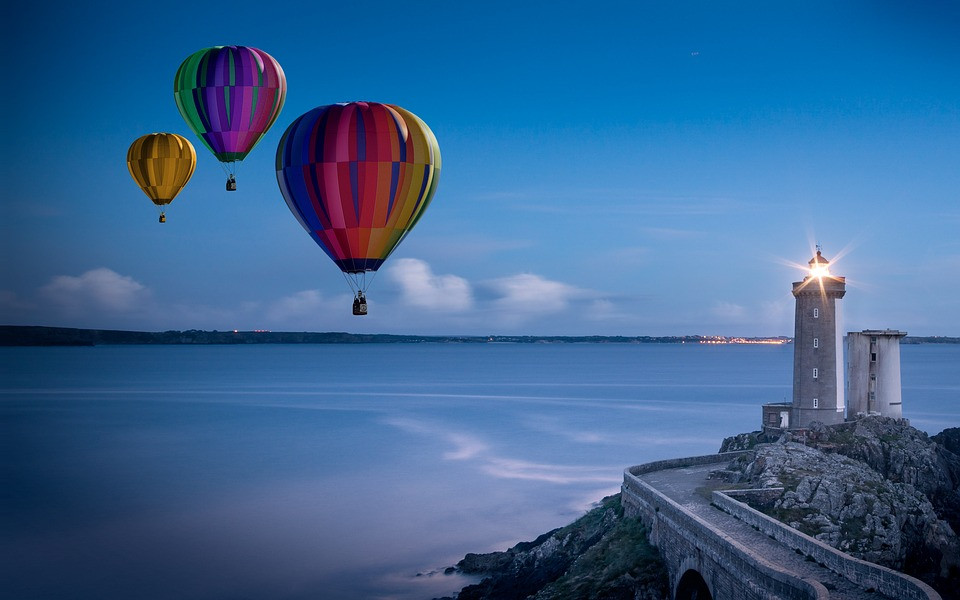
\includegraphics[width=7cm]{montgolfieres}};
    \def\x{10}
    \node (probas) at (\x+0.5, 2) {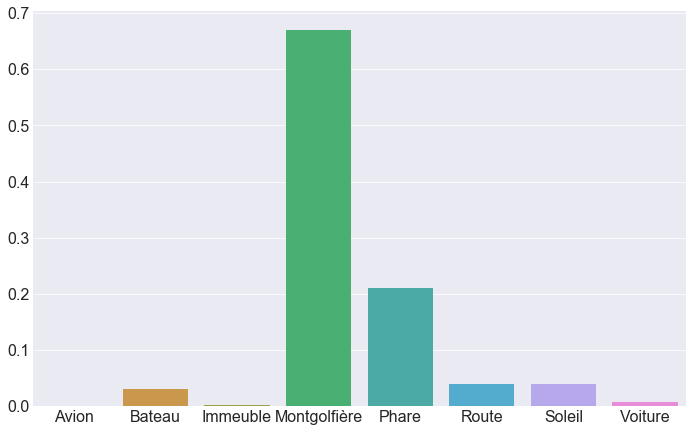
\includegraphics[width=6cm]{montgolfieres_probas}};
    \node (segmentation) at (\x-0.5, -2) {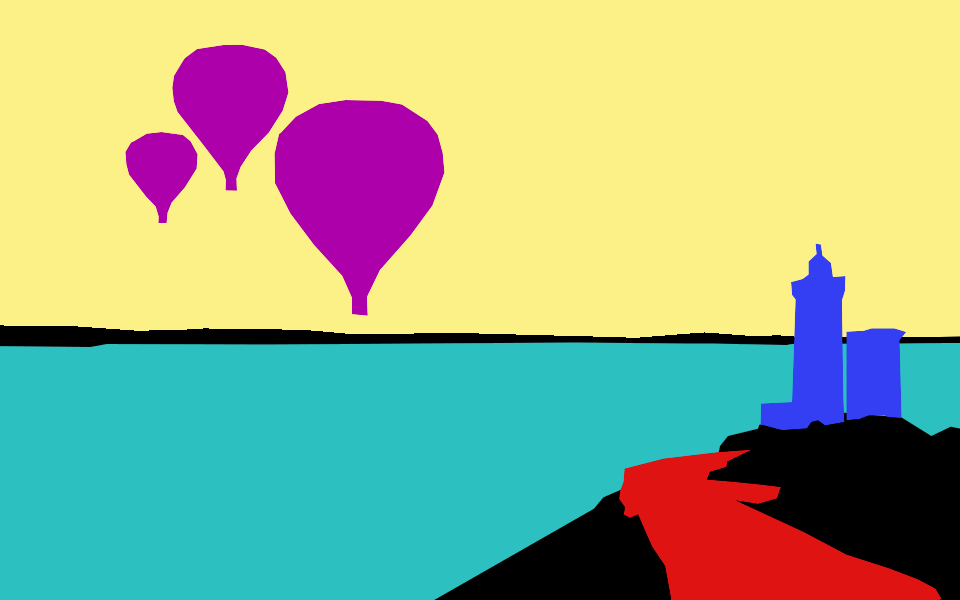
\includegraphics[width=3.8cm]{montgolfieres_segmentation}};
    \node [minimum width=2.1cm, fill=lpurple] at (\x+2.5, -1) {\footnotesize \textcolor{white}{Montgolfière}};
    \node [minimum width=2.1cm, fill=lyellow] at (\x+2.5, -1.5) {\footnotesize Ciel};
    \node [minimum width=2.1cm, fill=lcyan] at (\x+2.5, -2) {\footnotesize Eau};
    \node [minimum width=2.1cm, fill=lblue] at (\x+2.5, -2.5) {\footnotesize \textcolor{white}{Bâtiment}};
    \node [minimum width=2.1cm, fill=lred] at (\x+2.5, -3) {\footnotesize Route};
    \node[below] at (probas.south) {Classification};
    \node[below] at (segmentation.south) {Segmentation};
    \node[below] at (input.south) {Image};
    \draw (input) edge[in=180,out=0,->,ultra thick] (probas);
    \draw (input) edge[in=180,out=0,->,ultra thick] (segmentation);
  \end{tikzpicture}
\end{document}
}
  \caption{Exemple de classification et de segmentation sur une même image. La classification s'intéresse à la reconnaissance d'objet pour toute l'image, tandis que la segmentation opère sur chaque pixel. {\small Crédits image\,: \href{https://pixabay.com/en/balloon-hot-air-balloon-ride-mission-2331488/}{PIRO4D (CC0)}}.}
  \label{fig:classif_vs_seg}
\end{figure}

La segmentation d'image est une des premières tâches envisagées dans le cadre de la vision artificielle.
La légende veut que \textsc{Minsky} en 1964 ait demandé à un ses étudiants, Gerald \textsc{Sussman}, de \og passer l'été à connecter une caméra à un ordinateur et réussir à faire en sorte que l'ordinateur décrive ce qu'il voit \fg\footnote{``\emph{spend the summer linking a camera to a computer and getting the computer to describe what it saw}'', tel que rapporté par ~\citet{szeliski_computer_2011}, citant lui-même~\citet{boden_mind_2008} reprenant~\citet{crevier_ai_1993}.}.
La tâche envisagée par \textsc{Minsky} et \textsc{Papert} pour le \emph{Summer Vision Project} (cf.~\cref{fig:introductions}) consistait notamment à \og construire un système de programmes divisant une image issue d'un tube dissecteur\footnote{En référence au \emph{vidisector}, le dissecteur d'images inventé par Philo \textsc{Farnsworth} en 1927 sur le principe du tube cathodique. L'appareil reçoit de la lumière, ce qui stimule une photocathode et émet des électrons, produisant un signal électrique permettant de représenter l'image. C'est l'inverse de l'écran de télévision.} en différentes régions telles que\,: plutôt des objets, plutôt l'arrière-plan, ou du chaos\fg{} avec pour objectif final un logiciel réalisant \og l'identification d'objets, qui nommera chaque objet en les faisant correspondre avec un vocabulaire d'objets connus.\fg{}~\cite{papert_summer_1966}
Dès le départ, la reconnaissance de formes s'intéresse donc au découpage sémantique des images afin de comprendre les scènes visuelles qu'elles représentent.
Si cette tâche paraît triviale pour un humain, elle représente pourtant un défi considérable pour la machine. L'équipe de \textsc{Minsky} se heurte rapidement au paradoxe de ~\citet{moravec_mind_1988}\,: \og il est relativement aisé de mettre des ordinateurs au niveau d'un humain adulte dans le cadre d'un test d'intelligence ou d'une partie de dames, mais difficile voire impossible de leur donner les capacités de perception et la mobilité d'un bébé\fg{}\footnote{\emph{``it is comparatively easy to make computers exhibit adult level performance on intelligence tests or playing checkers, and difficult or impossible to give them the skills of a one-year-old when it comes to perception and mobility''}}.

De nombreux travaux se sont dès lors penchés sur le problème de la reconnaissance d'objet, c'est-à-dire l'identification d'un objet présent dans une image. On parlera ici de classification d'images, une tâche consistant à associer une image à un type d'objet. Cette tâche a concentré la majorité des efforts de la communauté, de l'utilisation de descripteurs \emph{ad hoc}~\cite{ullman_aligning_1989} aux caractéristiques apprises~\cite{vidal-naquet_object_2003} en passant par les modèles probabilistes~\cite{schneiderman_probabilistic_1998}. L'arrivée récente de grandes bases de données d'images annotées comme CIFAR-10 et CIFAR-100~\cite{krizhevsky_learning_2009}, puis ImageNet~\cite{deng_imagenet_2009,russakovsky_imagenet_2015} ont notamment permis d'aboutir au succès des réseaux convolutifs profonds en classification de chiffres sur la base de données MNIST~\cite{lecun_gradient-based_1998}, en reconnaissance de panneaux de signalisation~\cite{stallkamp_german_2011}, en identification de caractères chinois~\cite{liu_icdar_2011} et bien sûr en reconnaissance d'objets en tout genre sur ImageNet~\cite{krizhevsky_imagenet_2012}.

\begin{figure}[t]
  \resizebox{\textwidth}{!}{
    \documentclass{standalone}
\usepackage[utf8]{inputenc}
\usepackage[T1]{fontenc}
\usepackage{tikz}
\usepackage{ifthen}
%%%%%%%%%%%%%%%%%%%%%%%%%%%%%%%%%%%%%%%%
%           Commandes perso            %
%%%%%%%%%%%%%%%%%%%%%%%%%%%%%%%%%%%%%%%%

%% Figures centrées, et en position 'here, top, bottom or page'
\newenvironment{figureth}{%
		\begin{figure}[htbp]
			\centering
	}{
		\end{figure}
		}


%% Tableaux centrés, et en position 'here, top, bottom or page'
\newenvironment{tableth}{%
		\begin{table}[htbp]
			\centering
			%\rowcolors{1}{coleurtableau}{coleurtableau}
	}{
		\end{table}
		}

%% Sous-figures centrées, en position 'top'
\newenvironment{subfigureth}[1]{%
	\begin{subfigure}[t]{#1}
	\centering
}{
	\end{subfigure}
}

\newcommand{\citationChap}[2]{%
	\epigraph{\og \textit{#1} \fg{}}{#2}
}

%% On commence par une page impaire quand on change le style de numérotation de pages
\let\oldpagenumbering\pagenumbering
\renewcommand{\pagenumbering}[1]{%
	\cleardoublepage
	\oldpagenumbering{#1}
}

%% Légende du dataset ISPRS
\newcommand\isprslegende{
Légende\,: \textcolor{Black}{blanc}\,: routes, \textcolor{Blue}{bleu}\,: bâtiments, \textcolor{Cerulean}{cyan}\,: végétation basse, \textcolor{OliveGreen}{vert}\,: arbres, \textcolor{Dandelion}{jaune}\,: véhicules, \textcolor{BrickRed}{rouge}\,: autre.
}

%% Dessiner des réseaux de neurones avec Tikz
\newcommand{\convlayer}[9]{%{h}{w}{d}{name}{color}{x}{y}{z}%{note w}{note h}{note d}
   \def\h{#1}
   \def\w{#2}
   \def\d{#3}
   \def\name{#4}
   \ifthenelse {\equal{#5} {}} {\def\col{white}} {\def\col{#5}}
   \def\x{#6}
   \ifthenelse {\equal{#7} {}} {\def\y{0}} {\def\y{#7}}
   \ifthenelse {\equal{#8} {}} {\def\z{0}} {\def\z{#8}}
   % ne faites pas ça chez vous !
   \ifthenelse {\equal{#9} {}} {\convlayercontinued{}{}{}} {\convlayercontinued#9}
}

\newcommand\convlayercontinued[3]{
   \def\notew{#1}
   \def\noteh{#2}
   \def\noted{#3}
   \coordinate (A) at (\x-\d/2,  \y-\h/2, \z-\w/2);
   \coordinate (B) at (\x-\d/2,  \y-\h/2, \z+\w/2);
   \coordinate (C) at (\x-\d/2,  \y+\h/2, \z+\w/2);
   \coordinate (D) at (\x-\d/2,  \y+\h/2, \z-\w/2);
   \coordinate (E) at (\x+\d/2,  \y-\h/2, \z-\w/2);
   \coordinate (F) at (\x+\d/2,  \y-\h/2, \z+\w/2);
   \coordinate (G) at (\x+\d/2,  \y+\h/2, \z+\w/2);
   \coordinate (H) at (\x+\d/2,  \y+\h/2, \z-\w/2);

    \draw [draw opacity=0.3, fill opacity=0.8, fill=\col!60!white] (A) -- (B) -- (C) -- (D) -- cycle;
    \draw [draw opacity=0.3, fill opacity=0.8, fill=\col!60!white] (A) -- (B) -- (F) -- (E) -- cycle;
    % Face haut
    %\draw [left color=\col!60!white, right color=\col!80!white, shading=axis, shading angle=180] (C) -- (D)  -- (H) -- (G) -- cycle;
    \draw [fill opacity=0.9, fill=\col!70!white] (C) -- node[rotate=45,above] {\small \name} (D) -- (H) -- (G) -- cycle;
    %\draw [fill opacity=0.9, fill=\col!70!white] (C) -- (D) -- node[above] {\small \name} (H) -- (G) -- cycle;
    % Face droite
    \draw [fill opacity=0.9, fill=\col!60!white] (E) -- node[pos=0.75,rotate=45,below] {\scriptsize \notew} (F) -- (G) --  (H) -- cycle;
    % Face avant
    %\draw [shading=axis, left color=\col!60!white, right color=\col!40!white, shading angle=-45] (B) -- node[above,rotate=90] {\scriptsize \noteh} (C) -- (G) -- (F) -- node[below] {\scriptsize \noted}  cycle;
    \draw [fill opacity=0.9, fill=\col!50!white] (B) -- node[above,rotate=90] {\scriptsize \noteh} (C) -- (G) -- (F) -- node[below] {\scriptsize \noted}  cycle;
}

\newcommand{\fclayer}[8]{%{h}{w}{name}{color}{x}{y}{z}
   \def\h{#1}
   \def\w{#2}
   \def\name{#3}
   \ifthenelse {\equal{#4} {}} {\def\col{white}} {\def\col{#4}}
   \def\x{#5}
   \def\y{#6}
   \def\z{#7}
   \def\note{#8}
   \coordinate (A) at (\x-\w/2,  \y-\h/2, \z);
   \coordinate (B) at (\x+\w/2,  \y-\h/2, \z);
   \coordinate (C) at (\x+\w/2,  \y+\h/2, \z);
   \coordinate (D) at (\x-\w/2,  \y+\h/2, \z);

   \pgfmathparse{4*\w}\let\boxwidth\pgfmathresult
    \draw [fill=\col] (A) -- node[below,text width=\boxwidth cm,align=center] {\scriptsize \note} (B) -- (C) -- (D) -- cycle;

    \node (N) at ($(A)!0.5!(B)+(0,-1,0)$) {\name};
}

\newcommand{\alexnet}[4]{%{scale}{x}{y}{z}
  \def\scale{#1}
  \def\alexx{#2}
  \def\alexy{#3}
  \def\alexz{#4}


  \def\coblue{blue!50!white}
  \def\fcgrey{gray!50!white}

  \convlayer{1.3*\scale}{1.3*\scale}{0.02*\scale}{Image}{\coblue}{\alexx}{\alexy}{\alexz}{{227}{227}{3}}
  \convlayer{1.1*\scale}{1.1*\scale}{0.08*\scale}{Conv1}{\coblue}{\alexx+0.7*\scale}{\alexy}{\alexz}{{55}{55}{96}}
  \convlayer{0.7*\scale}{0.7*\scale}{0.5*\scale}{Conv2}{\coblue}{\alexx+1.5*\scale}{\alexy}{\alexz}{{27}{27}{256}}
  \convlayer{0.5*\scale}{0.5*\scale}{0.8*\scale}{Conv3}{\coblue}{\alexx+2.6*\scale}{\alexy}{\alexz}{{13}{13}{384}}
  \convlayer{0.5*\scale}{0.5*\scale}{0.8*\scale}{Conv4}{\coblue}{\alexx+3.8*\scale}{\alexy}{\alexz}{{13}{13}{384}}
  \convlayer{0.5*\scale}{0.5*\scale}{0.5*\scale}{Conv5}{\coblue}{\alexx+4.8*\scale}{\alexy}{\alexz}{{13}{13}{256}}
  \fclayer{\scale}{0.1*\scale}{FC1}{\fcgrey}{\alexx+5.4*\scale}{\alexy}{\alexz}{4096}
  \fclayer{\scale}{0.1*\scale}{FC2}{\fcgrey}{\alexx+5.7*\scale}{\alexy}{\alexz}{4096}
  \fclayer{\scale}{0.1*\scale}{FC3}{\fcgrey}{\alexx+6.0*\scale}{\alexy}{\alexz}{1000}
}

\newcommand{\imagelayer}[7]{%{width}{x}{y}{z}{path}{text_up}{text_down}
    \pgfmathparse{#1}\let\w\pgfmathresult
    \begin{scope}[canvas is yz plane at x=#2]
     \node[transform shape] (source) at (#3, #4) {\includegraphics[angle=-90,width=\w cm]{#5}};
    \end{scope}
     \node [transform shape, rotate=45, above] at (source.east) {#6};
     \node [transform shape, rotate=45, below] at (source.west) {\scriptsize{#7}};
}

\def\fourier{\mathcal{F}}

\newcommand{\lightspectrum}{%
\pgfplotsset{
    % this *defines* a custom colormap ...
    colormap={slategraywhite}{color(0cm)=(red); color(1cm)=(red); color(2cm)=(red); color(3cm)=(red); color(4cm)=(orange); color(5cm)=(yellow); color(6cm)=(green); color(7cm)=(blue); color(8cm)=(blue); color(9cm)=(purple); color(10cm)=(purple); color(12cm)=(black)}
}
\node at (1.5, 2.7) {\small 1mm};
\node at (4, 3) {Infrarouge};
\node at (7.75, 2.7) {\small 800nm};
\node at (9, 3) {Visible};
\node at (10.5, 2.7) {\small 400nm};
\node at (12, 3) {Ultraviolet};
\node at (13.5, 2.7) {\small 10nm};
\draw[->] (1, 2.5) -- (14, 2.5);
\begin{axis}[hide axis,width=16cm,height=4cm,colormap name=slategraywhite]
\addplot[domain=20:1000,samples=1500,ultra thick, point meta=x*x,mesh]{sin(x*x/80)};
\end{axis}
}

% Union généralisée
\newcommand{\wbigcup}{\mathop{\bigcup}\displaylimits}

\newcommand{\res}[2]{#1 {\footnotesize $\pm$ #2}}
\newcommand{\bres}[2]{\textbf{#1} {\footnotesize $\pm$ #2}}
\newcommand{\bbres}[2]{\res{\textit{#1}}{#2}}

\newcommand{\drawkernel}[9]{
\begin{tikzpicture}
	\draw[step=1cm,gray!50!white,very thin] (0,0) grid (3,3);
	\kernelnode{0.5}{0.5}{#1};
	\kernelnode{0.5}{1.5}{#2};
	\kernelnode{0.5}{2.5}{#3};
	\kernelnode{1.5}{0.5}{#4};
	\kernelnode{1.5}{1.5}{#5};
	\kernelnode{1.5}{2.5}{#6};
	\kernelnode{2.5}{0.5}{#7};
	\kernelnode{2.5}{1.5}{#8};
	\kernelnode{2.5}{2.5}{#9};
\end{tikzpicture}
}

\newcommand{\kernelnode}[3]{%{x}{y}{value}
	\ifthenelse{\equal{#3}{0}}{
		\def\kcolor{gray}
	}{
		\def\kcolor{black}
	}
	\node[\kcolor] at (#1, #2) {#3};
}

\newcommand{\chapsummary}[1]{
\section*{Résumé du chapitre :}
\parbox{0.9\linewidth}{
\setlength{\parindent}{4ex}
#1}
}

\newcommand{\eqname}[1]{\tag*{\small (#1)}}


\begin{document}
  \begin{tikzpicture}
  \usetikzlibrary{calc}
  \usetikzlibrary{3d}

  \def\scale{3}
  \def\netx{0}
  \def\nety{0}
  \def\netz{0}

  \def\coblue{blue!50!gray}
  \def\coorange{orange!50!gray}
  \def\cogreen{green!50!gray}
  \def\copurple{purple!50!white}

  \imagelayer{1.3*\scale}{0.05*\scale+\netx}{\nety}{\netz}{nobu_gray}{Image}{$32\times32\times1$}
  \convlayer{1.1*\scale}{1.1*\scale}{0.1*\scale}{Conv1}{\coblue}{\netx+0.8*\scale}{\nety}{\netz}{{28}{28}{6}}
  \convlayer{0.7*\scale}{0.7*\scale}{0.1*\scale}{Pool1}{\coorange}{\netx+1.5*\scale}{\nety}{\netz}{{14}{14}{6}}
  \convlayer{0.7*\scale}{0.7*\scale}{0.4*\scale}{Conv2}{\coblue}{\netx+2.4*\scale}{\nety}{\netz}{{10}{10}{16}}
  \convlayer{0.5*\scale}{0.5*\scale}{0.1*\scale}{Pool2}{\coorange}{\netx+3.3*\scale}{\nety}{\netz}{{5}{5}{16}}
  \fclayer{\scale}{0.1*\scale}{FC1}{\copurple}{\netx+3.9*\scale}{\nety}{\netz}{120}
  \fclayer{\scale}{0.1*\scale}{FC2}{\copurple}{\netx+4.3*\scale}{\nety}{\netz}{80}
  \fclayer{0.8*\scale}{0.1*\scale}{FC3}{\copurple}{\netx+4.7*\scale}{\nety}{\netz}{10}
  \node (out) at (\netx+5.8*\scale,\nety) {\Large ``Chat''};
  \draw[->] (\netx+4.75*\scale,\nety) -- (out.west);

  \end{tikzpicture}
\end{document}

  }
  \caption[Architecture LeNet-5.]{Architecture LeNet-5~\cite{lecun_gradient-based_1998}.}
  \label{fig:lenet}
\end{figure}

L'architecture LeNet-5, développée par \citet{lecun_gradient-based_1998}, définit la structure de référence d'un \gls{CNN}. Elle consiste en deux couches convolutives suivies de trois couches entièrement connectées, comme illustré dans la~\cref{fig:lenet}. La partie convolutive du modèle réalise l'extraction de caractéristiques dans le domaine image, tandis que les couches entièrement connectées forment un perceptron multi-couche opérant sur une représentation vectorielle et réalisant la classification finale. Initialement, LeNet-5 a été développé pour la reconnaissance de chiffres manuscrits dans des images en niveaux de gris de dimensions $32\times32$. En comparaison de la taille de l'image, les filtres convolutifs utilisés sont relativement grands, les noyaux de convolution étant de taille $5\times5$. La première couche $C1$ comporte 6 noyaux, c'est-à-dire que six cartes d'activation sont générées. Elles sont sous-échantillonnées avec un pas de 2, puis transmises à la couche convolutive suivante $C2$. Chaque carte d'activation de $C1$ est filtrée par chaque noyau de convolution de la couche $C2$, qui en comporte 16. Les cartes sont à nouveau sous-échantillonnées, ce qui produit finalement 16 cartes d'activation $5\times5$. Celles-ci sont alors aplaties en un vecteur de taille $1\times400$, entièrement connecté à une première couche cachée de dimension $120$, puis à une seconde de dimension $84$.
Finalement, ce descripteur est entièrement connecté au vecteur de sortie de taille $10$, chaque activation correspondant à un des 10 chiffres possibles. La sortie est alors transformée par un \emph{softmax} permettant de minimiser une entropie croisée par rétro-propagation du gradient.

La présence des couches entièrement connectées, dont le nombre de neurones est fixé, impose aux cartes d'activation issues des couches convolutives d'être de la bonne dimension. Cette contrainte impose en cascade que la taille des images traitées par LeNet soit toujours la même. Utiliser des images d'autres dimensions nécessiterait de ré-entraîner des couches entièrement connectées avec le nombre adéquat de neurones. Ce défaut, dû à la présence des couches entièrement connectées, est partagé par la plupart des \gls{CNN}.

\begin{figure}[t]
  \resizebox{\textwidth}{!}{
    \documentclass{standalone}
\usepackage[utf8]{inputenc}
\usepackage[T1]{fontenc}
\usepackage{tikz}
\usepackage{ifthen}
%%%%%%%%%%%%%%%%%%%%%%%%%%%%%%%%%%%%%%%%
%           Commandes perso            %
%%%%%%%%%%%%%%%%%%%%%%%%%%%%%%%%%%%%%%%%

%% Figures centrées, et en position 'here, top, bottom or page'
\newenvironment{figureth}{%
		\begin{figure}[htbp]
			\centering
	}{
		\end{figure}
		}


%% Tableaux centrés, et en position 'here, top, bottom or page'
\newenvironment{tableth}{%
		\begin{table}[htbp]
			\centering
			%\rowcolors{1}{coleurtableau}{coleurtableau}
	}{
		\end{table}
		}

%% Sous-figures centrées, en position 'top'
\newenvironment{subfigureth}[1]{%
	\begin{subfigure}[t]{#1}
	\centering
}{
	\end{subfigure}
}

\newcommand{\citationChap}[2]{%
	\epigraph{\og \textit{#1} \fg{}}{#2}
}

%% On commence par une page impaire quand on change le style de numérotation de pages
\let\oldpagenumbering\pagenumbering
\renewcommand{\pagenumbering}[1]{%
	\cleardoublepage
	\oldpagenumbering{#1}
}

%% Légende du dataset ISPRS
\newcommand\isprslegende{
Légende\,: \textcolor{Black}{blanc}\,: routes, \textcolor{Blue}{bleu}\,: bâtiments, \textcolor{Cerulean}{cyan}\,: végétation basse, \textcolor{OliveGreen}{vert}\,: arbres, \textcolor{Dandelion}{jaune}\,: véhicules, \textcolor{BrickRed}{rouge}\,: autre.
}

%% Dessiner des réseaux de neurones avec Tikz
\newcommand{\convlayer}[9]{%{h}{w}{d}{name}{color}{x}{y}{z}%{note w}{note h}{note d}
   \def\h{#1}
   \def\w{#2}
   \def\d{#3}
   \def\name{#4}
   \ifthenelse {\equal{#5} {}} {\def\col{white}} {\def\col{#5}}
   \def\x{#6}
   \ifthenelse {\equal{#7} {}} {\def\y{0}} {\def\y{#7}}
   \ifthenelse {\equal{#8} {}} {\def\z{0}} {\def\z{#8}}
   % ne faites pas ça chez vous !
   \ifthenelse {\equal{#9} {}} {\convlayercontinued{}{}{}} {\convlayercontinued#9}
}

\newcommand\convlayercontinued[3]{
   \def\notew{#1}
   \def\noteh{#2}
   \def\noted{#3}
   \coordinate (A) at (\x-\d/2,  \y-\h/2, \z-\w/2);
   \coordinate (B) at (\x-\d/2,  \y-\h/2, \z+\w/2);
   \coordinate (C) at (\x-\d/2,  \y+\h/2, \z+\w/2);
   \coordinate (D) at (\x-\d/2,  \y+\h/2, \z-\w/2);
   \coordinate (E) at (\x+\d/2,  \y-\h/2, \z-\w/2);
   \coordinate (F) at (\x+\d/2,  \y-\h/2, \z+\w/2);
   \coordinate (G) at (\x+\d/2,  \y+\h/2, \z+\w/2);
   \coordinate (H) at (\x+\d/2,  \y+\h/2, \z-\w/2);

    \draw [draw opacity=0.3, fill opacity=0.8, fill=\col!60!white] (A) -- (B) -- (C) -- (D) -- cycle;
    \draw [draw opacity=0.3, fill opacity=0.8, fill=\col!60!white] (A) -- (B) -- (F) -- (E) -- cycle;
    % Face haut
    %\draw [left color=\col!60!white, right color=\col!80!white, shading=axis, shading angle=180] (C) -- (D)  -- (H) -- (G) -- cycle;
    \draw [fill opacity=0.9, fill=\col!70!white] (C) -- node[rotate=45,above] {\small \name} (D) -- (H) -- (G) -- cycle;
    %\draw [fill opacity=0.9, fill=\col!70!white] (C) -- (D) -- node[above] {\small \name} (H) -- (G) -- cycle;
    % Face droite
    \draw [fill opacity=0.9, fill=\col!60!white] (E) -- node[pos=0.75,rotate=45,below] {\scriptsize \notew} (F) -- (G) --  (H) -- cycle;
    % Face avant
    %\draw [shading=axis, left color=\col!60!white, right color=\col!40!white, shading angle=-45] (B) -- node[above,rotate=90] {\scriptsize \noteh} (C) -- (G) -- (F) -- node[below] {\scriptsize \noted}  cycle;
    \draw [fill opacity=0.9, fill=\col!50!white] (B) -- node[above,rotate=90] {\scriptsize \noteh} (C) -- (G) -- (F) -- node[below] {\scriptsize \noted}  cycle;
}

\newcommand{\fclayer}[8]{%{h}{w}{name}{color}{x}{y}{z}
   \def\h{#1}
   \def\w{#2}
   \def\name{#3}
   \ifthenelse {\equal{#4} {}} {\def\col{white}} {\def\col{#4}}
   \def\x{#5}
   \def\y{#6}
   \def\z{#7}
   \def\note{#8}
   \coordinate (A) at (\x-\w/2,  \y-\h/2, \z);
   \coordinate (B) at (\x+\w/2,  \y-\h/2, \z);
   \coordinate (C) at (\x+\w/2,  \y+\h/2, \z);
   \coordinate (D) at (\x-\w/2,  \y+\h/2, \z);

   \pgfmathparse{4*\w}\let\boxwidth\pgfmathresult
    \draw [fill=\col] (A) -- node[below,text width=\boxwidth cm,align=center] {\scriptsize \note} (B) -- (C) -- (D) -- cycle;

    \node (N) at ($(A)!0.5!(B)+(0,-1,0)$) {\name};
}

\newcommand{\alexnet}[4]{%{scale}{x}{y}{z}
  \def\scale{#1}
  \def\alexx{#2}
  \def\alexy{#3}
  \def\alexz{#4}


  \def\coblue{blue!50!white}
  \def\fcgrey{gray!50!white}

  \convlayer{1.3*\scale}{1.3*\scale}{0.02*\scale}{Image}{\coblue}{\alexx}{\alexy}{\alexz}{{227}{227}{3}}
  \convlayer{1.1*\scale}{1.1*\scale}{0.08*\scale}{Conv1}{\coblue}{\alexx+0.7*\scale}{\alexy}{\alexz}{{55}{55}{96}}
  \convlayer{0.7*\scale}{0.7*\scale}{0.5*\scale}{Conv2}{\coblue}{\alexx+1.5*\scale}{\alexy}{\alexz}{{27}{27}{256}}
  \convlayer{0.5*\scale}{0.5*\scale}{0.8*\scale}{Conv3}{\coblue}{\alexx+2.6*\scale}{\alexy}{\alexz}{{13}{13}{384}}
  \convlayer{0.5*\scale}{0.5*\scale}{0.8*\scale}{Conv4}{\coblue}{\alexx+3.8*\scale}{\alexy}{\alexz}{{13}{13}{384}}
  \convlayer{0.5*\scale}{0.5*\scale}{0.5*\scale}{Conv5}{\coblue}{\alexx+4.8*\scale}{\alexy}{\alexz}{{13}{13}{256}}
  \fclayer{\scale}{0.1*\scale}{FC1}{\fcgrey}{\alexx+5.4*\scale}{\alexy}{\alexz}{4096}
  \fclayer{\scale}{0.1*\scale}{FC2}{\fcgrey}{\alexx+5.7*\scale}{\alexy}{\alexz}{4096}
  \fclayer{\scale}{0.1*\scale}{FC3}{\fcgrey}{\alexx+6.0*\scale}{\alexy}{\alexz}{1000}
}

\newcommand{\imagelayer}[7]{%{width}{x}{y}{z}{path}{text_up}{text_down}
    \pgfmathparse{#1}\let\w\pgfmathresult
    \begin{scope}[canvas is yz plane at x=#2]
     \node[transform shape] (source) at (#3, #4) {\includegraphics[angle=-90,width=\w cm]{#5}};
    \end{scope}
     \node [transform shape, rotate=45, above] at (source.east) {#6};
     \node [transform shape, rotate=45, below] at (source.west) {\scriptsize{#7}};
}

\def\fourier{\mathcal{F}}

\newcommand{\lightspectrum}{%
\pgfplotsset{
    % this *defines* a custom colormap ...
    colormap={slategraywhite}{color(0cm)=(red); color(1cm)=(red); color(2cm)=(red); color(3cm)=(red); color(4cm)=(orange); color(5cm)=(yellow); color(6cm)=(green); color(7cm)=(blue); color(8cm)=(blue); color(9cm)=(purple); color(10cm)=(purple); color(12cm)=(black)}
}
\node at (1.5, 2.7) {\small 1mm};
\node at (4, 3) {Infrarouge};
\node at (7.75, 2.7) {\small 800nm};
\node at (9, 3) {Visible};
\node at (10.5, 2.7) {\small 400nm};
\node at (12, 3) {Ultraviolet};
\node at (13.5, 2.7) {\small 10nm};
\draw[->] (1, 2.5) -- (14, 2.5);
\begin{axis}[hide axis,width=16cm,height=4cm,colormap name=slategraywhite]
\addplot[domain=20:1000,samples=1500,ultra thick, point meta=x*x,mesh]{sin(x*x/80)};
\end{axis}
}

% Union généralisée
\newcommand{\wbigcup}{\mathop{\bigcup}\displaylimits}

\newcommand{\res}[2]{#1 {\footnotesize $\pm$ #2}}
\newcommand{\bres}[2]{\textbf{#1} {\footnotesize $\pm$ #2}}
\newcommand{\bbres}[2]{\res{\textit{#1}}{#2}}

\newcommand{\drawkernel}[9]{
\begin{tikzpicture}
	\draw[step=1cm,gray!50!white,very thin] (0,0) grid (3,3);
	\kernelnode{0.5}{0.5}{#1};
	\kernelnode{0.5}{1.5}{#2};
	\kernelnode{0.5}{2.5}{#3};
	\kernelnode{1.5}{0.5}{#4};
	\kernelnode{1.5}{1.5}{#5};
	\kernelnode{1.5}{2.5}{#6};
	\kernelnode{2.5}{0.5}{#7};
	\kernelnode{2.5}{1.5}{#8};
	\kernelnode{2.5}{2.5}{#9};
\end{tikzpicture}
}

\newcommand{\kernelnode}[3]{%{x}{y}{value}
	\ifthenelse{\equal{#3}{0}}{
		\def\kcolor{gray}
	}{
		\def\kcolor{black}
	}
	\node[\kcolor] at (#1, #2) {#3};
}

\newcommand{\chapsummary}[1]{
\section*{Résumé du chapitre :}
\parbox{0.9\linewidth}{
\setlength{\parindent}{4ex}
#1}
}

\newcommand{\eqname}[1]{\tag*{\small (#1)}}


\begin{document}
  \begin{tikzpicture}
  \usetikzlibrary{calc}
  \usetikzlibrary{3d}

  \def\scale{4}
  \def\alexx{0}
  \def\alexy{0}
  \def\alexz{0}

  \def\coblue{blue!50!gray}
  \def\coorange{orange!50!gray}
  \def\cogreen{green!50!gray}
  \def\copurple{purple!50!white}

  \imagelayer{1.3*\scale}{0.*\scale+\alexx}{\alexy}{\alexz}{nobu}{Image}{$224\times224\times3$}
  \convlayer{1.1*\scale}{1.1*\scale}{0.1*\scale}{Conv1}{\coblue}{\alexx+0.6*\scale}{\alexy}{\alexz}{{55}{55}{96}}
  \convlayer{0.7*\scale}{0.7*\scale}{0.1*\scale}{Pool1}{\coorange}{\alexx+1*\scale}{\alexy}{\alexz}{{}{}{96}}
  \convlayer{0.7*\scale}{0.7*\scale}{0.1*\scale}{LRN}{\cogreen}{\alexx+1.35*\scale}{\alexy}{\alexz}{{}{}{96}}
  \convlayer{0.7*\scale}{0.7*\scale}{0.4*\scale}{Conv2}{\coblue}{\alexx+2*\scale}{\alexy}{\alexz}{{27}{27}{256}}
  \convlayer{0.5*\scale}{0.5*\scale}{0.1*\scale}{Pool2}{\coorange}{\alexx+2.5*\scale}{\alexy}{\alexz}{{13}{13}{}}
  \convlayer{0.5*\scale}{0.5*\scale}{0.1*\scale}{LRN}{\cogreen}{\alexx+2.75*\scale}{\alexy}{\alexz}{{}{}{}}
  \convlayer{0.5*\scale}{0.5*\scale}{0.6*\scale}{Conv3}{\coblue}{\alexx+3.35*\scale}{\alexy}{\alexz}{{}{}{384}}
  \convlayer{0.5*\scale}{0.5*\scale}{0.6*\scale}{Conv4}{\coblue}{\alexx+4.2*\scale}{\alexy}{\alexz}{{}{}{384}}
  \convlayer{0.5*\scale}{0.5*\scale}{0.4*\scale}{Conv5}{\coblue}{\alexx+5*\scale}{\alexy}{\alexz}{{}{}{256}}
  \convlayer{0.3*\scale}{0.3*\scale}{0.1*\scale}{Pool5}{\coorange}{\alexx+5.5*\scale}{\alexy}{\alexz}{{7}{7}{256}}
  \fclayer{\scale}{0.1*\scale}{FC1}{\copurple}{\alexx+5.8*\scale}{\alexy}{\alexz}{4096}
  \fclayer{\scale}{0.1*\scale}{FC2}{\copurple}{\alexx+6.05*\scale}{\alexy}{\alexz}{4096}
  \fclayer{0.8*\scale}{0.1*\scale}{FC3}{\copurple}{\alexx+6.3*\scale}{\alexy}{\alexz}{1000}
  \node (out) at (\alexx+6.7*\scale,\alexy) {\Large ``Chat''};
  \draw[->] (\alexx+6.35*\scale,\alexy) -- (out.west);

  \end{tikzpicture}
\end{document}

  }
  \caption[Architecture AlexNet]{Architecture AlexNet~\cite{krizhevsky_imagenet_2012}.}
  \label{fig:alexnet}
\end{figure}

Pour le traitement des images en couleur, le réseau AlexNet~\cite{krizhevsky_imagenet_2012} utilise une approche similaire. Ce modèle, détaillé dans la~\cref{fig:alexnet} comporte 8 couches, dont 5 convolutives, et traite des images \gls{RVB} de dimensions $224\times224$. La première convolution utilise un grand noyau de dimensions $11\times11$ et précède un sous-échantillonnage, ce qui réduit fortement les dimensions de l'image. Ainsi, les cartes d'activation en sortie de la première couche sont de dimensions $96\times27\times27$, puis $256\times13\times13$ après la seconde. Une normalisation \gls{LRN} est appliquée après les deux premières convolutions pour favoriser la généralisation du modèle. La structure convolutive d'AlexNet est conçue de telle sorte à ce que le nombre de cartes d'activation augmente de façon inversement proportionnelle à la réduction des dimensions spatiales. Cela permet de conserver un nombre raisonnable de valeurs à calculer tout en accroissant l'expressivité de la représentation apprise. Les trois couches de convolution suivantes sont finalement sous-échantillonnées afin de produire 256 cartes de caractéristiques de dimensions $6\times6$, transformées en un vecteur de longueur $9216$.
Les couches entièrement connectées le réduisent alors à 2048 puis le projettent dans un vecteur de classification de taille 1000, correspondant aux classes d'ImageNet~\cite{deng_imagenet_2009}. Ce modèle a permis à~\citet{krizhevsky_imagenet_2012} de remporter la compétition \gls{ILSVRC}~\cite{russakovsky_imagenet_2015} en 2012 avec un taux d'erreur de 15,3\% en considérant les 5 prédictions les plus probables.

\citet{zeiler_visualizing_2014} se sont penchés sur l'architecture AlexNet afin d'établir un diagnostic de ses points forts et de ses points faibles. En particulier, ils proposent d'inverser les opérations de convolution afin de pouvoir relier les représentations internes aux pixels de l'image originale. Ils définissent ainsi les opérations transposées de la couche de convolution et du sous-échantillonnage et construisent un \emph{Deconvnet} permettant de visualiser les caractéristiques apprises par AlexNet. En outre, ils étudient attentivement les filtres convolutifs appris par les couches basses du réseau. Leurs travaux mettent en évidence plusieurs propriétés intéressantes. La première est que les caractéristiques des couches supérieures présentent une plus grande invariance aux transformations géométriques et colorimétriques de bas niveau, traduisant ainsi un niveau d'abstraction plus élevé. La seconde est que les deux premières couches convolutives d'AlexNet contiennent des filtres liés aux hautes et basses fréquences, mais conservent peu d'information des fréquences intermédiaires. Ils proposent ainsi de remplacer la première couche, dont les noyaux sont de dimension $11\times11$, par des filtres $7\times7$ appliqués sur l'image avec un pas de 2 plutôt qu'un pas de 4, afin de conserver plus d'information. Leurs filtres appris de cette façon présentent une meilleure variété et moins de filtres ``morts'' à très faible amplitude. Enfin, la visualisation des représentations internes permet de constater que celles-ci ne sont pas aléatoires, mais possèdent bien une sémantique liée à la discrimination des objets, certains neurones se focalisant par exemple sur les visages, d'autres sur les roues, etc.

\begin{figure}[t]
  \resizebox{\textwidth}{!}{
    \documentclass{standalone}
\usepackage[utf8]{inputenc}
\usepackage[T1]{fontenc}
\usepackage{tikz}
\usepackage{ifthen}
%%%%%%%%%%%%%%%%%%%%%%%%%%%%%%%%%%%%%%%%
%           Commandes perso            %
%%%%%%%%%%%%%%%%%%%%%%%%%%%%%%%%%%%%%%%%

%% Figures centrées, et en position 'here, top, bottom or page'
\newenvironment{figureth}{%
		\begin{figure}[htbp]
			\centering
	}{
		\end{figure}
		}


%% Tableaux centrés, et en position 'here, top, bottom or page'
\newenvironment{tableth}{%
		\begin{table}[htbp]
			\centering
			%\rowcolors{1}{coleurtableau}{coleurtableau}
	}{
		\end{table}
		}

%% Sous-figures centrées, en position 'top'
\newenvironment{subfigureth}[1]{%
	\begin{subfigure}[t]{#1}
	\centering
}{
	\end{subfigure}
}

\newcommand{\citationChap}[2]{%
	\epigraph{\og \textit{#1} \fg{}}{#2}
}

%% On commence par une page impaire quand on change le style de numérotation de pages
\let\oldpagenumbering\pagenumbering
\renewcommand{\pagenumbering}[1]{%
	\cleardoublepage
	\oldpagenumbering{#1}
}

%% Légende du dataset ISPRS
\newcommand\isprslegende{
Légende\,: \textcolor{Black}{blanc}\,: routes, \textcolor{Blue}{bleu}\,: bâtiments, \textcolor{Cerulean}{cyan}\,: végétation basse, \textcolor{OliveGreen}{vert}\,: arbres, \textcolor{Dandelion}{jaune}\,: véhicules, \textcolor{BrickRed}{rouge}\,: autre.
}

%% Dessiner des réseaux de neurones avec Tikz
\newcommand{\convlayer}[9]{%{h}{w}{d}{name}{color}{x}{y}{z}%{note w}{note h}{note d}
   \def\h{#1}
   \def\w{#2}
   \def\d{#3}
   \def\name{#4}
   \ifthenelse {\equal{#5} {}} {\def\col{white}} {\def\col{#5}}
   \def\x{#6}
   \ifthenelse {\equal{#7} {}} {\def\y{0}} {\def\y{#7}}
   \ifthenelse {\equal{#8} {}} {\def\z{0}} {\def\z{#8}}
   % ne faites pas ça chez vous !
   \ifthenelse {\equal{#9} {}} {\convlayercontinued{}{}{}} {\convlayercontinued#9}
}

\newcommand\convlayercontinued[3]{
   \def\notew{#1}
   \def\noteh{#2}
   \def\noted{#3}
   \coordinate (A) at (\x-\d/2,  \y-\h/2, \z-\w/2);
   \coordinate (B) at (\x-\d/2,  \y-\h/2, \z+\w/2);
   \coordinate (C) at (\x-\d/2,  \y+\h/2, \z+\w/2);
   \coordinate (D) at (\x-\d/2,  \y+\h/2, \z-\w/2);
   \coordinate (E) at (\x+\d/2,  \y-\h/2, \z-\w/2);
   \coordinate (F) at (\x+\d/2,  \y-\h/2, \z+\w/2);
   \coordinate (G) at (\x+\d/2,  \y+\h/2, \z+\w/2);
   \coordinate (H) at (\x+\d/2,  \y+\h/2, \z-\w/2);

    \draw [draw opacity=0.3, fill opacity=0.8, fill=\col!60!white] (A) -- (B) -- (C) -- (D) -- cycle;
    \draw [draw opacity=0.3, fill opacity=0.8, fill=\col!60!white] (A) -- (B) -- (F) -- (E) -- cycle;
    % Face haut
    %\draw [left color=\col!60!white, right color=\col!80!white, shading=axis, shading angle=180] (C) -- (D)  -- (H) -- (G) -- cycle;
    \draw [fill opacity=0.9, fill=\col!70!white] (C) -- node[rotate=45,above] {\small \name} (D) -- (H) -- (G) -- cycle;
    %\draw [fill opacity=0.9, fill=\col!70!white] (C) -- (D) -- node[above] {\small \name} (H) -- (G) -- cycle;
    % Face droite
    \draw [fill opacity=0.9, fill=\col!60!white] (E) -- node[pos=0.75,rotate=45,below] {\scriptsize \notew} (F) -- (G) --  (H) -- cycle;
    % Face avant
    %\draw [shading=axis, left color=\col!60!white, right color=\col!40!white, shading angle=-45] (B) -- node[above,rotate=90] {\scriptsize \noteh} (C) -- (G) -- (F) -- node[below] {\scriptsize \noted}  cycle;
    \draw [fill opacity=0.9, fill=\col!50!white] (B) -- node[above,rotate=90] {\scriptsize \noteh} (C) -- (G) -- (F) -- node[below] {\scriptsize \noted}  cycle;
}

\newcommand{\fclayer}[8]{%{h}{w}{name}{color}{x}{y}{z}
   \def\h{#1}
   \def\w{#2}
   \def\name{#3}
   \ifthenelse {\equal{#4} {}} {\def\col{white}} {\def\col{#4}}
   \def\x{#5}
   \def\y{#6}
   \def\z{#7}
   \def\note{#8}
   \coordinate (A) at (\x-\w/2,  \y-\h/2, \z);
   \coordinate (B) at (\x+\w/2,  \y-\h/2, \z);
   \coordinate (C) at (\x+\w/2,  \y+\h/2, \z);
   \coordinate (D) at (\x-\w/2,  \y+\h/2, \z);

   \pgfmathparse{4*\w}\let\boxwidth\pgfmathresult
    \draw [fill=\col] (A) -- node[below,text width=\boxwidth cm,align=center] {\scriptsize \note} (B) -- (C) -- (D) -- cycle;

    \node (N) at ($(A)!0.5!(B)+(0,-1,0)$) {\name};
}

\newcommand{\alexnet}[4]{%{scale}{x}{y}{z}
  \def\scale{#1}
  \def\alexx{#2}
  \def\alexy{#3}
  \def\alexz{#4}


  \def\coblue{blue!50!white}
  \def\fcgrey{gray!50!white}

  \convlayer{1.3*\scale}{1.3*\scale}{0.02*\scale}{Image}{\coblue}{\alexx}{\alexy}{\alexz}{{227}{227}{3}}
  \convlayer{1.1*\scale}{1.1*\scale}{0.08*\scale}{Conv1}{\coblue}{\alexx+0.7*\scale}{\alexy}{\alexz}{{55}{55}{96}}
  \convlayer{0.7*\scale}{0.7*\scale}{0.5*\scale}{Conv2}{\coblue}{\alexx+1.5*\scale}{\alexy}{\alexz}{{27}{27}{256}}
  \convlayer{0.5*\scale}{0.5*\scale}{0.8*\scale}{Conv3}{\coblue}{\alexx+2.6*\scale}{\alexy}{\alexz}{{13}{13}{384}}
  \convlayer{0.5*\scale}{0.5*\scale}{0.8*\scale}{Conv4}{\coblue}{\alexx+3.8*\scale}{\alexy}{\alexz}{{13}{13}{384}}
  \convlayer{0.5*\scale}{0.5*\scale}{0.5*\scale}{Conv5}{\coblue}{\alexx+4.8*\scale}{\alexy}{\alexz}{{13}{13}{256}}
  \fclayer{\scale}{0.1*\scale}{FC1}{\fcgrey}{\alexx+5.4*\scale}{\alexy}{\alexz}{4096}
  \fclayer{\scale}{0.1*\scale}{FC2}{\fcgrey}{\alexx+5.7*\scale}{\alexy}{\alexz}{4096}
  \fclayer{\scale}{0.1*\scale}{FC3}{\fcgrey}{\alexx+6.0*\scale}{\alexy}{\alexz}{1000}
}

\newcommand{\imagelayer}[7]{%{width}{x}{y}{z}{path}{text_up}{text_down}
    \pgfmathparse{#1}\let\w\pgfmathresult
    \begin{scope}[canvas is yz plane at x=#2]
     \node[transform shape] (source) at (#3, #4) {\includegraphics[angle=-90,width=\w cm]{#5}};
    \end{scope}
     \node [transform shape, rotate=45, above] at (source.east) {#6};
     \node [transform shape, rotate=45, below] at (source.west) {\scriptsize{#7}};
}

\def\fourier{\mathcal{F}}

\newcommand{\lightspectrum}{%
\pgfplotsset{
    % this *defines* a custom colormap ...
    colormap={slategraywhite}{color(0cm)=(red); color(1cm)=(red); color(2cm)=(red); color(3cm)=(red); color(4cm)=(orange); color(5cm)=(yellow); color(6cm)=(green); color(7cm)=(blue); color(8cm)=(blue); color(9cm)=(purple); color(10cm)=(purple); color(12cm)=(black)}
}
\node at (1.5, 2.7) {\small 1mm};
\node at (4, 3) {Infrarouge};
\node at (7.75, 2.7) {\small 800nm};
\node at (9, 3) {Visible};
\node at (10.5, 2.7) {\small 400nm};
\node at (12, 3) {Ultraviolet};
\node at (13.5, 2.7) {\small 10nm};
\draw[->] (1, 2.5) -- (14, 2.5);
\begin{axis}[hide axis,width=16cm,height=4cm,colormap name=slategraywhite]
\addplot[domain=20:1000,samples=1500,ultra thick, point meta=x*x,mesh]{sin(x*x/80)};
\end{axis}
}

% Union généralisée
\newcommand{\wbigcup}{\mathop{\bigcup}\displaylimits}

\newcommand{\res}[2]{#1 {\footnotesize $\pm$ #2}}
\newcommand{\bres}[2]{\textbf{#1} {\footnotesize $\pm$ #2}}
\newcommand{\bbres}[2]{\res{\textit{#1}}{#2}}

\newcommand{\drawkernel}[9]{
\begin{tikzpicture}
	\draw[step=1cm,gray!50!white,very thin] (0,0) grid (3,3);
	\kernelnode{0.5}{0.5}{#1};
	\kernelnode{0.5}{1.5}{#2};
	\kernelnode{0.5}{2.5}{#3};
	\kernelnode{1.5}{0.5}{#4};
	\kernelnode{1.5}{1.5}{#5};
	\kernelnode{1.5}{2.5}{#6};
	\kernelnode{2.5}{0.5}{#7};
	\kernelnode{2.5}{1.5}{#8};
	\kernelnode{2.5}{2.5}{#9};
\end{tikzpicture}
}

\newcommand{\kernelnode}[3]{%{x}{y}{value}
	\ifthenelse{\equal{#3}{0}}{
		\def\kcolor{gray}
	}{
		\def\kcolor{black}
	}
	\node[\kcolor] at (#1, #2) {#3};
}

\newcommand{\chapsummary}[1]{
\section*{Résumé du chapitre :}
\parbox{0.9\linewidth}{
\setlength{\parindent}{4ex}
#1}
}

\newcommand{\eqname}[1]{\tag*{\small (#1)}}


\begin{document}
  \begin{tikzpicture}
  \usetikzlibrary{calc}
  \usetikzlibrary{3d}

  \def\scale{3.5}
  \def\vggx{0}
  \def\vggy{0}
  \def\vggz{0}

  \def\coblue{blue!50!gray}
  \def\coorange{orange!70!gray}
  \def\cogreen{green!50!gray}
  \def\copurple{purple!50!white}

  \imagelayer{1.3*\scale}{0.1*\scale+\vggx}{\vggy}{\vggz}{nobu}{Image}{$224\times224\times3$}
  \convlayer{1.1*\scale}{1.1*\scale}{0.04*\scale}{Conv1-2}{\coblue}{\vggx+0.6*\scale}{\vggy}{\vggz}{{}{}{64}}
  \convlayer{1.1*\scale}{1.1*\scale}{0.04*\scale}{}{\coblue}{\vggx+0.7*\scale}{\vggy}{\vggz}{{}{}{64}}
  \convlayer{0.8*\scale}{0.8*\scale}{0.04*\scale}{Pool1}{\coorange}{\vggx+1*\scale}{\vggy}{\vggz}{{112}{112}{}}
  \convlayer{0.8*\scale}{0.8*\scale}{0.08*\scale}{Conv3-4}{\coblue}{\vggx+1.2*\scale}{\vggy}{\vggz}{{}{}{128}}
  \convlayer{0.8*\scale}{0.8*\scale}{0.08*\scale}{}{\coblue}{\vggx+1.35*\scale}{\vggy}{\vggz}{{112}{}{128}}
  \convlayer{0.6*\scale}{0.6*\scale}{0.08*\scale}{Pool2}{\coorange}{\vggx+1.7*\scale}{\vggy}{\vggz}{{}{56}{}}
  \convlayer{0.6*\scale}{0.6*\scale}{0.2*\scale}{Conv5-7}{\coblue}{\vggx+2*\scale}{\vggy}{\vggz}{{}{}{256}}
  \convlayer{0.6*\scale}{0.6*\scale}{0.2*\scale}{}{\coblue}{\vggx+2.25*\scale}{\vggy}{\vggz}{{}{}{256}}
  \convlayer{0.6*\scale}{0.6*\scale}{0.2*\scale}{}{\coblue}{\vggx+2.5*\scale}{\vggy}{\vggz}{{56}{}{256}}
  \convlayer{0.3*\scale}{0.3*\scale}{0.2*\scale}{Pool3}{\coorange}{\vggx+2.9*\scale}{\vggy}{\vggz}{{28}{28}{}}
  \convlayer{0.3*\scale}{0.3*\scale}{0.4*\scale}{Conv8-10}{\coblue}{\vggx+3.4*\scale}{\vggy}{\vggz}{{}{}{512}}
  \convlayer{0.3*\scale}{0.3*\scale}{0.4*\scale}{}{\coblue}{\vggx+3.9*\scale}{\vggy}{\vggz}{{}{}{512}}
  \convlayer{0.3*\scale}{0.3*\scale}{0.4*\scale}{}{\coblue}{\vggx+4.4*\scale}{\vggy}{\vggz}{{14}{}{512}}
  \convlayer{0.3*\scale}{0.3*\scale}{0.2*\scale}{Pool4}{\coorange}{\vggx+4.95*\scale}{\vggy}{\vggz}{{14}{14}{}}
  \convlayer{0.3*\scale}{0.3*\scale}{0.4*\scale}{Conv11-13}{\coblue}{\vggx+5.45*\scale}{\vggy}{\vggz}{{}{}{512}}
  \convlayer{0.3*\scale}{0.3*\scale}{0.4*\scale}{}{\coblue}{\vggx+5.95*\scale}{\vggy}{\vggz}{{}{}{512}}
  \convlayer{0.3*\scale}{0.3*\scale}{0.4*\scale}{}{\coblue}{\vggx+6.45*\scale}{\vggy}{\vggz}{{14}{}{512}}
  \convlayer{0.15*\scale}{0.15*\scale}{0.4*\scale}{Pool5}{\coorange}{\vggx+7.05*\scale}{\vggy}{\vggz}{{7}{7}{512}}

  \fclayer{\scale}{0.1*\scale}{FC1}{\copurple}{\vggx+7.4*\scale}{\vggy}{\vggz}{4096}
  \fclayer{\scale}{0.1*\scale}{FC2}{\copurple}{\vggx+7.6*\scale}{\vggy}{\vggz}{4096}
  \fclayer{0.8*\scale}{0.1*\scale}{FC3}{\copurple}{\vggx+7.8*\scale}{\vggy}{\vggz}{1000}
  \node (out) at (\vggx+8.2*\scale,\vggy) {\Large ``Chat''};
  \draw[->] (\vggx+7.85*\scale,\vggy) -- (out.west);

  \end{tikzpicture}
\end{document}

  }
  \caption[Architecture VGG-16.]{Architecture VGG-16~\cite{simonyan_very_2014}.}
  \label{fig:vgg}
\end{figure}

Le modèle VGG-16 affine l'architecture en proposant notamment de réduire la dimension des noyaux de convolution. En effet, \citet{chatfield_return_2014,simonyan_very_2014} suggèrent qu'il est plus simple d'optimiser plusieurs convolutions successives de noyaux $3\times3$ qu'une unique convolution de dimension $11\times11$. En outre, la présence de non-linéarités supplémentaires est susceptible d'accroître l'expressivité du modèle. Le modèle VGG-16 remplace donc chaque convolution large classique par un bloc de 2 ou 3 convolutions $3\times3$ successives. Le modèle de référence VGG-16 comporte 16 couches dont 13 convolutives et 3 entièrement connectées, suivant l'approche canonique de LeNet et d'AlexNet. Il comporte 5 blocs convolutifs $3\times3$ chacun suivi d'un sous-échantillonnage de pas 2. Les deux premiers blocs comportent 2 couches de convolution, les trois suivants en comportant 3. Les cartes d'activation finales sont de dimension $512\times7\times7$, VGG-16 réalisant ainsi une réduction de dimension d'un facteur 32. Ce vecteur de longueur 25088 est ensuite réduit à 4096, puis aux 1000 classes d'intérêt d'ImageNet. Afin de limiter le surapprentissage, les couches entièrement connectées sont soumises au \emph{Dropout}. Ces améliorations proposées à l'architecture classique des \gls{CNN} ont permis d'obtenir en 2014 un taux d'erreur de 7,4\% en reconnaissance d'objet durant la compétition \gls{ILSVRC}.

\begin{figure}[t]
  \resizebox{\textwidth}{!}{
    \documentclass{standalone}
\usepackage[utf8]{inputenc}
\usepackage[T1]{fontenc}
\usepackage{tikz}
\usepackage{ifthen}
\usepackage{graphicx}
%%%%%%%%%%%%%%%%%%%%%%%%%%%%%%%%%%%%%%%%
%           Commandes perso            %
%%%%%%%%%%%%%%%%%%%%%%%%%%%%%%%%%%%%%%%%

%% Figures centrées, et en position 'here, top, bottom or page'
\newenvironment{figureth}{%
		\begin{figure}[htbp]
			\centering
	}{
		\end{figure}
		}


%% Tableaux centrés, et en position 'here, top, bottom or page'
\newenvironment{tableth}{%
		\begin{table}[htbp]
			\centering
			%\rowcolors{1}{coleurtableau}{coleurtableau}
	}{
		\end{table}
		}

%% Sous-figures centrées, en position 'top'
\newenvironment{subfigureth}[1]{%
	\begin{subfigure}[t]{#1}
	\centering
}{
	\end{subfigure}
}

\newcommand{\citationChap}[2]{%
	\epigraph{\og \textit{#1} \fg{}}{#2}
}

%% On commence par une page impaire quand on change le style de numérotation de pages
\let\oldpagenumbering\pagenumbering
\renewcommand{\pagenumbering}[1]{%
	\cleardoublepage
	\oldpagenumbering{#1}
}

%% Légende du dataset ISPRS
\newcommand\isprslegende{
Légende\,: \textcolor{Black}{blanc}\,: routes, \textcolor{Blue}{bleu}\,: bâtiments, \textcolor{Cerulean}{cyan}\,: végétation basse, \textcolor{OliveGreen}{vert}\,: arbres, \textcolor{Dandelion}{jaune}\,: véhicules, \textcolor{BrickRed}{rouge}\,: autre.
}

%% Dessiner des réseaux de neurones avec Tikz
\newcommand{\convlayer}[9]{%{h}{w}{d}{name}{color}{x}{y}{z}%{note w}{note h}{note d}
   \def\h{#1}
   \def\w{#2}
   \def\d{#3}
   \def\name{#4}
   \ifthenelse {\equal{#5} {}} {\def\col{white}} {\def\col{#5}}
   \def\x{#6}
   \ifthenelse {\equal{#7} {}} {\def\y{0}} {\def\y{#7}}
   \ifthenelse {\equal{#8} {}} {\def\z{0}} {\def\z{#8}}
   % ne faites pas ça chez vous !
   \ifthenelse {\equal{#9} {}} {\convlayercontinued{}{}{}} {\convlayercontinued#9}
}

\newcommand\convlayercontinued[3]{
   \def\notew{#1}
   \def\noteh{#2}
   \def\noted{#3}
   \coordinate (A) at (\x-\d/2,  \y-\h/2, \z-\w/2);
   \coordinate (B) at (\x-\d/2,  \y-\h/2, \z+\w/2);
   \coordinate (C) at (\x-\d/2,  \y+\h/2, \z+\w/2);
   \coordinate (D) at (\x-\d/2,  \y+\h/2, \z-\w/2);
   \coordinate (E) at (\x+\d/2,  \y-\h/2, \z-\w/2);
   \coordinate (F) at (\x+\d/2,  \y-\h/2, \z+\w/2);
   \coordinate (G) at (\x+\d/2,  \y+\h/2, \z+\w/2);
   \coordinate (H) at (\x+\d/2,  \y+\h/2, \z-\w/2);

    \draw [draw opacity=0.3, fill opacity=0.8, fill=\col!60!white] (A) -- (B) -- (C) -- (D) -- cycle;
    \draw [draw opacity=0.3, fill opacity=0.8, fill=\col!60!white] (A) -- (B) -- (F) -- (E) -- cycle;
    % Face haut
    %\draw [left color=\col!60!white, right color=\col!80!white, shading=axis, shading angle=180] (C) -- (D)  -- (H) -- (G) -- cycle;
    \draw [fill opacity=0.9, fill=\col!70!white] (C) -- node[rotate=45,above] {\small \name} (D) -- (H) -- (G) -- cycle;
    %\draw [fill opacity=0.9, fill=\col!70!white] (C) -- (D) -- node[above] {\small \name} (H) -- (G) -- cycle;
    % Face droite
    \draw [fill opacity=0.9, fill=\col!60!white] (E) -- node[pos=0.75,rotate=45,below] {\scriptsize \notew} (F) -- (G) --  (H) -- cycle;
    % Face avant
    %\draw [shading=axis, left color=\col!60!white, right color=\col!40!white, shading angle=-45] (B) -- node[above,rotate=90] {\scriptsize \noteh} (C) -- (G) -- (F) -- node[below] {\scriptsize \noted}  cycle;
    \draw [fill opacity=0.9, fill=\col!50!white] (B) -- node[above,rotate=90] {\scriptsize \noteh} (C) -- (G) -- (F) -- node[below] {\scriptsize \noted}  cycle;
}

\newcommand{\fclayer}[8]{%{h}{w}{name}{color}{x}{y}{z}
   \def\h{#1}
   \def\w{#2}
   \def\name{#3}
   \ifthenelse {\equal{#4} {}} {\def\col{white}} {\def\col{#4}}
   \def\x{#5}
   \def\y{#6}
   \def\z{#7}
   \def\note{#8}
   \coordinate (A) at (\x-\w/2,  \y-\h/2, \z);
   \coordinate (B) at (\x+\w/2,  \y-\h/2, \z);
   \coordinate (C) at (\x+\w/2,  \y+\h/2, \z);
   \coordinate (D) at (\x-\w/2,  \y+\h/2, \z);

   \pgfmathparse{4*\w}\let\boxwidth\pgfmathresult
    \draw [fill=\col] (A) -- node[below,text width=\boxwidth cm,align=center] {\scriptsize \note} (B) -- (C) -- (D) -- cycle;

    \node (N) at ($(A)!0.5!(B)+(0,-1,0)$) {\name};
}

\newcommand{\alexnet}[4]{%{scale}{x}{y}{z}
  \def\scale{#1}
  \def\alexx{#2}
  \def\alexy{#3}
  \def\alexz{#4}


  \def\coblue{blue!50!white}
  \def\fcgrey{gray!50!white}

  \convlayer{1.3*\scale}{1.3*\scale}{0.02*\scale}{Image}{\coblue}{\alexx}{\alexy}{\alexz}{{227}{227}{3}}
  \convlayer{1.1*\scale}{1.1*\scale}{0.08*\scale}{Conv1}{\coblue}{\alexx+0.7*\scale}{\alexy}{\alexz}{{55}{55}{96}}
  \convlayer{0.7*\scale}{0.7*\scale}{0.5*\scale}{Conv2}{\coblue}{\alexx+1.5*\scale}{\alexy}{\alexz}{{27}{27}{256}}
  \convlayer{0.5*\scale}{0.5*\scale}{0.8*\scale}{Conv3}{\coblue}{\alexx+2.6*\scale}{\alexy}{\alexz}{{13}{13}{384}}
  \convlayer{0.5*\scale}{0.5*\scale}{0.8*\scale}{Conv4}{\coblue}{\alexx+3.8*\scale}{\alexy}{\alexz}{{13}{13}{384}}
  \convlayer{0.5*\scale}{0.5*\scale}{0.5*\scale}{Conv5}{\coblue}{\alexx+4.8*\scale}{\alexy}{\alexz}{{13}{13}{256}}
  \fclayer{\scale}{0.1*\scale}{FC1}{\fcgrey}{\alexx+5.4*\scale}{\alexy}{\alexz}{4096}
  \fclayer{\scale}{0.1*\scale}{FC2}{\fcgrey}{\alexx+5.7*\scale}{\alexy}{\alexz}{4096}
  \fclayer{\scale}{0.1*\scale}{FC3}{\fcgrey}{\alexx+6.0*\scale}{\alexy}{\alexz}{1000}
}

\newcommand{\imagelayer}[7]{%{width}{x}{y}{z}{path}{text_up}{text_down}
    \pgfmathparse{#1}\let\w\pgfmathresult
    \begin{scope}[canvas is yz plane at x=#2]
     \node[transform shape] (source) at (#3, #4) {\includegraphics[angle=-90,width=\w cm]{#5}};
    \end{scope}
     \node [transform shape, rotate=45, above] at (source.east) {#6};
     \node [transform shape, rotate=45, below] at (source.west) {\scriptsize{#7}};
}

\def\fourier{\mathcal{F}}

\newcommand{\lightspectrum}{%
\pgfplotsset{
    % this *defines* a custom colormap ...
    colormap={slategraywhite}{color(0cm)=(red); color(1cm)=(red); color(2cm)=(red); color(3cm)=(red); color(4cm)=(orange); color(5cm)=(yellow); color(6cm)=(green); color(7cm)=(blue); color(8cm)=(blue); color(9cm)=(purple); color(10cm)=(purple); color(12cm)=(black)}
}
\node at (1.5, 2.7) {\small 1mm};
\node at (4, 3) {Infrarouge};
\node at (7.75, 2.7) {\small 800nm};
\node at (9, 3) {Visible};
\node at (10.5, 2.7) {\small 400nm};
\node at (12, 3) {Ultraviolet};
\node at (13.5, 2.7) {\small 10nm};
\draw[->] (1, 2.5) -- (14, 2.5);
\begin{axis}[hide axis,width=16cm,height=4cm,colormap name=slategraywhite]
\addplot[domain=20:1000,samples=1500,ultra thick, point meta=x*x,mesh]{sin(x*x/80)};
\end{axis}
}

% Union généralisée
\newcommand{\wbigcup}{\mathop{\bigcup}\displaylimits}

\newcommand{\res}[2]{#1 {\footnotesize $\pm$ #2}}
\newcommand{\bres}[2]{\textbf{#1} {\footnotesize $\pm$ #2}}
\newcommand{\bbres}[2]{\res{\textit{#1}}{#2}}

\newcommand{\drawkernel}[9]{
\begin{tikzpicture}
	\draw[step=1cm,gray!50!white,very thin] (0,0) grid (3,3);
	\kernelnode{0.5}{0.5}{#1};
	\kernelnode{0.5}{1.5}{#2};
	\kernelnode{0.5}{2.5}{#3};
	\kernelnode{1.5}{0.5}{#4};
	\kernelnode{1.5}{1.5}{#5};
	\kernelnode{1.5}{2.5}{#6};
	\kernelnode{2.5}{0.5}{#7};
	\kernelnode{2.5}{1.5}{#8};
	\kernelnode{2.5}{2.5}{#9};
\end{tikzpicture}
}

\newcommand{\kernelnode}[3]{%{x}{y}{value}
	\ifthenelse{\equal{#3}{0}}{
		\def\kcolor{gray}
	}{
		\def\kcolor{black}
	}
	\node[\kcolor] at (#1, #2) {#3};
}

\newcommand{\chapsummary}[1]{
\section*{Résumé du chapitre :}
\parbox{0.9\linewidth}{
\setlength{\parindent}{4ex}
#1}
}

\newcommand{\eqname}[1]{\tag*{\small (#1)}}


\begin{document}
  \begin{tikzpicture}
  \usetikzlibrary{calc}
  \usetikzlibrary{3d}

  \def\scale{4}
  \def\vggx{0}
  \def\vggy{0}
  \def\vggz{0}

  \def\coblue{blue!50!gray}
  \def\cored{red!50!gray}
  \def\coorange{orange!70!gray}
  \def\cogreen{green!50!gray}
  \def\copurple{purple!50!white}

  \imagelayer{1.3*\scale}{-0.3*\scale+\vggx}{\vggy}{\vggz}{nobu}{Image}{$224\times224\times3$}
  \convlayer{1.3*\scale}{1.3*\scale}{0.02*\scale}{Image}{\coblue}{0.2*\scale+\vggx}{\vggy}{\vggz}{{224}{}{3}}
  \convlayer{1*\scale}{1*\scale}{0.04*\scale}{Conv1}{\coblue}{\vggx+0.6*\scale}{\vggy}{\vggz}{{112}{112}{64}}
  \convlayer{0.8*\scale}{0.8*\scale}{0.04*\scale}{Pool1}{\coorange}{\vggx+1*\scale}{\vggy}{\vggz}{{56}{56}{}}
  \convlayer{0.8*\scale}{0.8*\scale}{0.15*\scale}{Conv2}{\coblue}{\vggx+1.4*\scale}{\vggy}{\vggz}{{}{}{192}}
  \convlayer{0.6*\scale}{0.6*\scale}{0.15*\scale}{Pool2}{\coorange}{\vggx+1.8*\scale}{\vggy}{\vggz}{{28}{28}{}}
  \node at (\vggx+2.45*\scale, \vggy+0.5*\scale) {Inception (3a-3b)};
  \convlayer{0.6*\scale}{0.6*\scale}{0.2*\scale}{}{\cored}{\vggx+2.2*\scale}{\vggy}{\vggz}{{}{}{256}}
  \convlayer{0.6*\scale}{0.6*\scale}{0.3*\scale}{}{\cored}{\vggx+2.5*\scale}{\vggy}{\vggz}{{}{}{480}}
  \convlayer{0.4*\scale}{0.4*\scale}{0.3*\scale}{Pool3}{\coorange}{\vggx+2.9*\scale}{\vggy}{\vggz}{{14}{14}{}}
  \node at (\vggx+4.5*\scale, \vggy+0.4*\scale) {Inception (4a-4e)};
  \convlayer{0.4*\scale}{0.4*\scale}{0.4*\scale}{}{\cored}{\vggx+3.4*\scale}{\vggy}{\vggz}{{}{}{512}}
  \convlayer{0.4*\scale}{0.4*\scale}{0.4*\scale}{}{\cored}{\vggx+3.9*\scale}{\vggy}{\vggz}{{}{}{512}}
  \convlayer{0.4*\scale}{0.4*\scale}{0.4*\scale}{}{\cored}{\vggx+4.4*\scale}{\vggy}{\vggz}{{}{}{512}}
  \convlayer{0.4*\scale}{0.4*\scale}{0.4*\scale}{}{\cored}{\vggx+4.9*\scale}{\vggy}{\vggz}{{}{}{528}}
  \convlayer{0.4*\scale}{0.4*\scale}{0.5*\scale}{}{\cored}{\vggx+5.4*\scale}{\vggy}{\vggz}{{}{}{832}}
  \convlayer{0.3*\scale}{0.3*\scale}{0.5*\scale}{Pool5}{\coorange}{\vggx+6.1*\scale}{\vggy}{\vggz}{{}{}{832}}
  \node at (\vggx+7*\scale, \vggy+0.4*\scale) {Inception (5a-5b)};
  \convlayer{0.3*\scale}{0.3*\scale}{0.5*\scale}{}{\cored}{\vggx+6.7*\scale}{\vggy}{\vggz}{{}{}{832}}
  \convlayer{0.3*\scale}{0.3*\scale}{0.6*\scale}{}{\cored}{\vggx+7.3*\scale}{\vggy}{\vggz}{{}{}{1024}}
  \node at (\vggx+8.05*\scale, \vggy+0.2*\scale) {Avg. pool};
  \convlayer{0.1*\scale}{0.1*\scale}{0.6*\scale}{}{\coorange}{\vggx+8.05*\scale}{\vggy}{\vggz}{{}{}{$1\times1\times1024$}}
  \fclayer{\scale}{0.1*\scale}{FC}{\copurple}{\vggx+8.5*\scale}{\vggy}{\vggz}{1000}
  \node (out) at (\vggx+8.9*\scale,\vggy) {\Large ``Chat''};
  \draw[->] (\vggx+8.55*\scale,\vggy) -- (out.west);

  \end{tikzpicture}
\end{document}

  }
  \caption[Architecture GoogLeNet.]{Architecture GoogLeNet~\cite{szegedy_going_2015}.}
  \label{fig:googlenet}
\end{figure}

\begin{figure}
  \begin{minipage}{0.48\textwidth}
    \resizebox{\textwidth}{!}{
      \documentclass{standalone}
\usepackage[utf8]{inputenc}
\usepackage[T1]{fontenc}
\usepackage{tikz}
\usepackage{ifthen}
%%%%%%%%%%%%%%%%%%%%%%%%%%%%%%%%%%%%%%%%
%           Commandes perso            %
%%%%%%%%%%%%%%%%%%%%%%%%%%%%%%%%%%%%%%%%

%% Figures centrées, et en position 'here, top, bottom or page'
\newenvironment{figureth}{%
		\begin{figure}[htbp]
			\centering
	}{
		\end{figure}
		}


%% Tableaux centrés, et en position 'here, top, bottom or page'
\newenvironment{tableth}{%
		\begin{table}[htbp]
			\centering
			%\rowcolors{1}{coleurtableau}{coleurtableau}
	}{
		\end{table}
		}

%% Sous-figures centrées, en position 'top'
\newenvironment{subfigureth}[1]{%
	\begin{subfigure}[t]{#1}
	\centering
}{
	\end{subfigure}
}

\newcommand{\citationChap}[2]{%
	\epigraph{\og \textit{#1} \fg{}}{#2}
}

%% On commence par une page impaire quand on change le style de numérotation de pages
\let\oldpagenumbering\pagenumbering
\renewcommand{\pagenumbering}[1]{%
	\cleardoublepage
	\oldpagenumbering{#1}
}

%% Légende du dataset ISPRS
\newcommand\isprslegende{
Légende\,: \textcolor{Black}{blanc}\,: routes, \textcolor{Blue}{bleu}\,: bâtiments, \textcolor{Cerulean}{cyan}\,: végétation basse, \textcolor{OliveGreen}{vert}\,: arbres, \textcolor{Dandelion}{jaune}\,: véhicules, \textcolor{BrickRed}{rouge}\,: autre.
}

%% Dessiner des réseaux de neurones avec Tikz
\newcommand{\convlayer}[9]{%{h}{w}{d}{name}{color}{x}{y}{z}%{note w}{note h}{note d}
   \def\h{#1}
   \def\w{#2}
   \def\d{#3}
   \def\name{#4}
   \ifthenelse {\equal{#5} {}} {\def\col{white}} {\def\col{#5}}
   \def\x{#6}
   \ifthenelse {\equal{#7} {}} {\def\y{0}} {\def\y{#7}}
   \ifthenelse {\equal{#8} {}} {\def\z{0}} {\def\z{#8}}
   % ne faites pas ça chez vous !
   \ifthenelse {\equal{#9} {}} {\convlayercontinued{}{}{}} {\convlayercontinued#9}
}

\newcommand\convlayercontinued[3]{
   \def\notew{#1}
   \def\noteh{#2}
   \def\noted{#3}
   \coordinate (A) at (\x-\d/2,  \y-\h/2, \z-\w/2);
   \coordinate (B) at (\x-\d/2,  \y-\h/2, \z+\w/2);
   \coordinate (C) at (\x-\d/2,  \y+\h/2, \z+\w/2);
   \coordinate (D) at (\x-\d/2,  \y+\h/2, \z-\w/2);
   \coordinate (E) at (\x+\d/2,  \y-\h/2, \z-\w/2);
   \coordinate (F) at (\x+\d/2,  \y-\h/2, \z+\w/2);
   \coordinate (G) at (\x+\d/2,  \y+\h/2, \z+\w/2);
   \coordinate (H) at (\x+\d/2,  \y+\h/2, \z-\w/2);

    \draw [draw opacity=0.3, fill opacity=0.8, fill=\col!60!white] (A) -- (B) -- (C) -- (D) -- cycle;
    \draw [draw opacity=0.3, fill opacity=0.8, fill=\col!60!white] (A) -- (B) -- (F) -- (E) -- cycle;
    % Face haut
    %\draw [left color=\col!60!white, right color=\col!80!white, shading=axis, shading angle=180] (C) -- (D)  -- (H) -- (G) -- cycle;
    \draw [fill opacity=0.9, fill=\col!70!white] (C) -- node[rotate=45,above] {\small \name} (D) -- (H) -- (G) -- cycle;
    %\draw [fill opacity=0.9, fill=\col!70!white] (C) -- (D) -- node[above] {\small \name} (H) -- (G) -- cycle;
    % Face droite
    \draw [fill opacity=0.9, fill=\col!60!white] (E) -- node[pos=0.75,rotate=45,below] {\scriptsize \notew} (F) -- (G) --  (H) -- cycle;
    % Face avant
    %\draw [shading=axis, left color=\col!60!white, right color=\col!40!white, shading angle=-45] (B) -- node[above,rotate=90] {\scriptsize \noteh} (C) -- (G) -- (F) -- node[below] {\scriptsize \noted}  cycle;
    \draw [fill opacity=0.9, fill=\col!50!white] (B) -- node[above,rotate=90] {\scriptsize \noteh} (C) -- (G) -- (F) -- node[below] {\scriptsize \noted}  cycle;
}

\newcommand{\fclayer}[8]{%{h}{w}{name}{color}{x}{y}{z}
   \def\h{#1}
   \def\w{#2}
   \def\name{#3}
   \ifthenelse {\equal{#4} {}} {\def\col{white}} {\def\col{#4}}
   \def\x{#5}
   \def\y{#6}
   \def\z{#7}
   \def\note{#8}
   \coordinate (A) at (\x-\w/2,  \y-\h/2, \z);
   \coordinate (B) at (\x+\w/2,  \y-\h/2, \z);
   \coordinate (C) at (\x+\w/2,  \y+\h/2, \z);
   \coordinate (D) at (\x-\w/2,  \y+\h/2, \z);

   \pgfmathparse{4*\w}\let\boxwidth\pgfmathresult
    \draw [fill=\col] (A) -- node[below,text width=\boxwidth cm,align=center] {\scriptsize \note} (B) -- (C) -- (D) -- cycle;

    \node (N) at ($(A)!0.5!(B)+(0,-1,0)$) {\name};
}

\newcommand{\alexnet}[4]{%{scale}{x}{y}{z}
  \def\scale{#1}
  \def\alexx{#2}
  \def\alexy{#3}
  \def\alexz{#4}


  \def\coblue{blue!50!white}
  \def\fcgrey{gray!50!white}

  \convlayer{1.3*\scale}{1.3*\scale}{0.02*\scale}{Image}{\coblue}{\alexx}{\alexy}{\alexz}{{227}{227}{3}}
  \convlayer{1.1*\scale}{1.1*\scale}{0.08*\scale}{Conv1}{\coblue}{\alexx+0.7*\scale}{\alexy}{\alexz}{{55}{55}{96}}
  \convlayer{0.7*\scale}{0.7*\scale}{0.5*\scale}{Conv2}{\coblue}{\alexx+1.5*\scale}{\alexy}{\alexz}{{27}{27}{256}}
  \convlayer{0.5*\scale}{0.5*\scale}{0.8*\scale}{Conv3}{\coblue}{\alexx+2.6*\scale}{\alexy}{\alexz}{{13}{13}{384}}
  \convlayer{0.5*\scale}{0.5*\scale}{0.8*\scale}{Conv4}{\coblue}{\alexx+3.8*\scale}{\alexy}{\alexz}{{13}{13}{384}}
  \convlayer{0.5*\scale}{0.5*\scale}{0.5*\scale}{Conv5}{\coblue}{\alexx+4.8*\scale}{\alexy}{\alexz}{{13}{13}{256}}
  \fclayer{\scale}{0.1*\scale}{FC1}{\fcgrey}{\alexx+5.4*\scale}{\alexy}{\alexz}{4096}
  \fclayer{\scale}{0.1*\scale}{FC2}{\fcgrey}{\alexx+5.7*\scale}{\alexy}{\alexz}{4096}
  \fclayer{\scale}{0.1*\scale}{FC3}{\fcgrey}{\alexx+6.0*\scale}{\alexy}{\alexz}{1000}
}

\newcommand{\imagelayer}[7]{%{width}{x}{y}{z}{path}{text_up}{text_down}
    \pgfmathparse{#1}\let\w\pgfmathresult
    \begin{scope}[canvas is yz plane at x=#2]
     \node[transform shape] (source) at (#3, #4) {\includegraphics[angle=-90,width=\w cm]{#5}};
    \end{scope}
     \node [transform shape, rotate=45, above] at (source.east) {#6};
     \node [transform shape, rotate=45, below] at (source.west) {\scriptsize{#7}};
}

\def\fourier{\mathcal{F}}

\newcommand{\lightspectrum}{%
\pgfplotsset{
    % this *defines* a custom colormap ...
    colormap={slategraywhite}{color(0cm)=(red); color(1cm)=(red); color(2cm)=(red); color(3cm)=(red); color(4cm)=(orange); color(5cm)=(yellow); color(6cm)=(green); color(7cm)=(blue); color(8cm)=(blue); color(9cm)=(purple); color(10cm)=(purple); color(12cm)=(black)}
}
\node at (1.5, 2.7) {\small 1mm};
\node at (4, 3) {Infrarouge};
\node at (7.75, 2.7) {\small 800nm};
\node at (9, 3) {Visible};
\node at (10.5, 2.7) {\small 400nm};
\node at (12, 3) {Ultraviolet};
\node at (13.5, 2.7) {\small 10nm};
\draw[->] (1, 2.5) -- (14, 2.5);
\begin{axis}[hide axis,width=16cm,height=4cm,colormap name=slategraywhite]
\addplot[domain=20:1000,samples=1500,ultra thick, point meta=x*x,mesh]{sin(x*x/80)};
\end{axis}
}

% Union généralisée
\newcommand{\wbigcup}{\mathop{\bigcup}\displaylimits}

\newcommand{\res}[2]{#1 {\footnotesize $\pm$ #2}}
\newcommand{\bres}[2]{\textbf{#1} {\footnotesize $\pm$ #2}}
\newcommand{\bbres}[2]{\res{\textit{#1}}{#2}}

\newcommand{\drawkernel}[9]{
\begin{tikzpicture}
	\draw[step=1cm,gray!50!white,very thin] (0,0) grid (3,3);
	\kernelnode{0.5}{0.5}{#1};
	\kernelnode{0.5}{1.5}{#2};
	\kernelnode{0.5}{2.5}{#3};
	\kernelnode{1.5}{0.5}{#4};
	\kernelnode{1.5}{1.5}{#5};
	\kernelnode{1.5}{2.5}{#6};
	\kernelnode{2.5}{0.5}{#7};
	\kernelnode{2.5}{1.5}{#8};
	\kernelnode{2.5}{2.5}{#9};
\end{tikzpicture}
}

\newcommand{\kernelnode}[3]{%{x}{y}{value}
	\ifthenelse{\equal{#3}{0}}{
		\def\kcolor{gray}
	}{
		\def\kcolor{black}
	}
	\node[\kcolor] at (#1, #2) {#3};
}

\newcommand{\chapsummary}[1]{
\section*{Résumé du chapitre :}
\parbox{0.9\linewidth}{
\setlength{\parindent}{4ex}
#1}
}

\newcommand{\eqname}[1]{\tag*{\small (#1)}}


\begin{document}
  \begin{tikzpicture}
  \usetikzlibrary{calc}
  \usetikzlibrary{3d}

  \def\scale{3}
  \def\netx{0}
  \def\nety{0}
  \def\netz{0}

  \def\coblue{blue!50!gray}
  \def\coorange{orange!70!gray}
  \def\cogreen{green!50!gray}
  \def\coyellow{yellow!50!white}
  \def\cored{red!50!white}

  \convlayer{1.3*\scale}{1.3*\scale}{0.6*\scale}{Carte d'activation}{white}{0.2*\scale+\netx}{\nety}{\netz}{{}{}{}}

  \draw (0.5*\scale+\netx, \nety) -- (1.0*\scale+\netx, \nety);
  \draw[->] (1.0*\scale+\netx, \nety) to[bend left=15] (1.8*\scale+\netx, 2.25*\scale+\nety); 
  \draw[->] (1.0*\scale+\netx, \nety) to[bend left=5] (1.8*\scale+\netx, 0.75*\scale+\nety); 
  \draw[->] (1.0*\scale+\netx, \nety) to[bend right=5] (1.8*\scale+\netx, -0.75*\scale+\nety); 
  \draw[->] (1.0*\scale+\netx, \nety) to[bend right=15] (1.8*\scale+\netx, -2.25*\scale+\nety); 

  \convlayer{1*\scale}{1*\scale}{0.1*\scale}{Conv $1\times1$}{\coblue}{\netx+2.0*\scale}{2.25*\scale+\nety}{\netz}{{}{}{}}
  \convlayer{1*\scale}{1*\scale}{0.3*\scale}{Conv $5\times5$}{\coyellow}{\netx+3.4*\scale}{2.25*\scale+\nety}{\netz}{{}{}{}}

  \convlayer{1*\scale}{1*\scale}{0.1*\scale}{Conv $1\times1$}{\coblue}{\netx+2.0*\scale}{0.75*\scale+\nety}{\netz}{{}{}{}}
  \convlayer{1*\scale}{1*\scale}{0.3*\scale}{Conv $3\times3$}{\cored}{\netx+3.4*\scale}{0.75*\scale+\nety}{\netz}{{}{}{}}

  \convlayer{1*\scale}{1*\scale}{1.0*\scale}{Pool $3\times3$}{\coorange}{\netx+2.2*\scale}{-0.75*\scale+\nety}{\netz}{{}{}{}}
  \convlayer{1*\scale}{1*\scale}{0.3*\scale}{Conv $1\times1$}{\cogreen}{\netx+3.4*\scale}{-0.75*\scale+\nety}{\netz}{{}{}{}}

  \convlayer{1*\scale}{1*\scale}{0.3*\scale}{Conv $1\times1$}{\coblue}{\netx+2.0*\scale}{-2.25*\scale+\nety}{\netz}{{}{}{}}


  \convlayer{1*\scale}{1*\scale}{0.3*\scale}{}{\cored}{\netx+5.0*\scale}{0*\scale+\nety}{\netz}{{}{}{}}
  \draw[->] (\netx+3.6*\scale, \nety+0.75*\scale, \netz) to[bend left=20] (\netx+5.0*\scale,\nety+0.5*\scale, \netz);


  \convlayer{1*\scale}{1*\scale}{0.3*\scale}{}{\coyellow}{\netx+5.3*\scale}{0*\scale+\nety}{\netz}{{}{}{}}
  \draw[->] (\netx+3.6*\scale, \nety+2.25*\scale, \netz) to[bend left=30] (\netx+5.3*\scale,\nety+0.5*\scale, \netz);


  \draw[->] (\netx+3.6*\scale, \nety-0.75*\scale, \netz) to[bend right=40] (\netx+5.6*\scale,\nety-0.5*\scale, \netz+0.25*\scale);
  \convlayer{1*\scale}{1*\scale}{0.3*\scale}{}{\cogreen}{\netx+5.6*\scale}{0*\scale+\nety}{\netz}{{}{}{}}


  \draw[->] (\netx+2.15*\scale, \nety-2.25*\scale, \netz) to[bend right=30] (\netx+5.9*\scale,\nety-0.5*\scale, \netz);
  \convlayer{1*\scale}{1*\scale}{0.3*\scale}{}{\coblue}{\netx+5.9*\scale}{0*\scale+\nety}{\netz}{{}{}{}}


  \node at (5.8*\scale, 0.8*\scale) {\large Concaténation};


  \end{tikzpicture}
\end{document}

    }
    \caption[Module \emph{Inception}.]{Module \emph{Inception}~\cite{szegedy_going_2015}.}
    \label{fig:inception}
  \end{minipage}
  \hfill
  \begin{minipage}{0.48\textwidth}
    \resizebox{\textwidth}{!}{
      \documentclass{standalone}
\usepackage[utf8]{inputenc}
\usepackage[T1]{fontenc}
\usepackage{tikz}
\usepackage{ifthen}
%%%%%%%%%%%%%%%%%%%%%%%%%%%%%%%%%%%%%%%%
%           Commandes perso            %
%%%%%%%%%%%%%%%%%%%%%%%%%%%%%%%%%%%%%%%%

%% Figures centrées, et en position 'here, top, bottom or page'
\newenvironment{figureth}{%
		\begin{figure}[htbp]
			\centering
	}{
		\end{figure}
		}


%% Tableaux centrés, et en position 'here, top, bottom or page'
\newenvironment{tableth}{%
		\begin{table}[htbp]
			\centering
			%\rowcolors{1}{coleurtableau}{coleurtableau}
	}{
		\end{table}
		}

%% Sous-figures centrées, en position 'top'
\newenvironment{subfigureth}[1]{%
	\begin{subfigure}[t]{#1}
	\centering
}{
	\end{subfigure}
}

\newcommand{\citationChap}[2]{%
	\epigraph{\og \textit{#1} \fg{}}{#2}
}

%% On commence par une page impaire quand on change le style de numérotation de pages
\let\oldpagenumbering\pagenumbering
\renewcommand{\pagenumbering}[1]{%
	\cleardoublepage
	\oldpagenumbering{#1}
}

%% Légende du dataset ISPRS
\newcommand\isprslegende{
Légende\,: \textcolor{Black}{blanc}\,: routes, \textcolor{Blue}{bleu}\,: bâtiments, \textcolor{Cerulean}{cyan}\,: végétation basse, \textcolor{OliveGreen}{vert}\,: arbres, \textcolor{Dandelion}{jaune}\,: véhicules, \textcolor{BrickRed}{rouge}\,: autre.
}

%% Dessiner des réseaux de neurones avec Tikz
\newcommand{\convlayer}[9]{%{h}{w}{d}{name}{color}{x}{y}{z}%{note w}{note h}{note d}
   \def\h{#1}
   \def\w{#2}
   \def\d{#3}
   \def\name{#4}
   \ifthenelse {\equal{#5} {}} {\def\col{white}} {\def\col{#5}}
   \def\x{#6}
   \ifthenelse {\equal{#7} {}} {\def\y{0}} {\def\y{#7}}
   \ifthenelse {\equal{#8} {}} {\def\z{0}} {\def\z{#8}}
   % ne faites pas ça chez vous !
   \ifthenelse {\equal{#9} {}} {\convlayercontinued{}{}{}} {\convlayercontinued#9}
}

\newcommand\convlayercontinued[3]{
   \def\notew{#1}
   \def\noteh{#2}
   \def\noted{#3}
   \coordinate (A) at (\x-\d/2,  \y-\h/2, \z-\w/2);
   \coordinate (B) at (\x-\d/2,  \y-\h/2, \z+\w/2);
   \coordinate (C) at (\x-\d/2,  \y+\h/2, \z+\w/2);
   \coordinate (D) at (\x-\d/2,  \y+\h/2, \z-\w/2);
   \coordinate (E) at (\x+\d/2,  \y-\h/2, \z-\w/2);
   \coordinate (F) at (\x+\d/2,  \y-\h/2, \z+\w/2);
   \coordinate (G) at (\x+\d/2,  \y+\h/2, \z+\w/2);
   \coordinate (H) at (\x+\d/2,  \y+\h/2, \z-\w/2);

    \draw [draw opacity=0.3, fill opacity=0.8, fill=\col!60!white] (A) -- (B) -- (C) -- (D) -- cycle;
    \draw [draw opacity=0.3, fill opacity=0.8, fill=\col!60!white] (A) -- (B) -- (F) -- (E) -- cycle;
    % Face haut
    %\draw [left color=\col!60!white, right color=\col!80!white, shading=axis, shading angle=180] (C) -- (D)  -- (H) -- (G) -- cycle;
    \draw [fill opacity=0.9, fill=\col!70!white] (C) -- node[rotate=45,above] {\small \name} (D) -- (H) -- (G) -- cycle;
    %\draw [fill opacity=0.9, fill=\col!70!white] (C) -- (D) -- node[above] {\small \name} (H) -- (G) -- cycle;
    % Face droite
    \draw [fill opacity=0.9, fill=\col!60!white] (E) -- node[pos=0.75,rotate=45,below] {\scriptsize \notew} (F) -- (G) --  (H) -- cycle;
    % Face avant
    %\draw [shading=axis, left color=\col!60!white, right color=\col!40!white, shading angle=-45] (B) -- node[above,rotate=90] {\scriptsize \noteh} (C) -- (G) -- (F) -- node[below] {\scriptsize \noted}  cycle;
    \draw [fill opacity=0.9, fill=\col!50!white] (B) -- node[above,rotate=90] {\scriptsize \noteh} (C) -- (G) -- (F) -- node[below] {\scriptsize \noted}  cycle;
}

\newcommand{\fclayer}[8]{%{h}{w}{name}{color}{x}{y}{z}
   \def\h{#1}
   \def\w{#2}
   \def\name{#3}
   \ifthenelse {\equal{#4} {}} {\def\col{white}} {\def\col{#4}}
   \def\x{#5}
   \def\y{#6}
   \def\z{#7}
   \def\note{#8}
   \coordinate (A) at (\x-\w/2,  \y-\h/2, \z);
   \coordinate (B) at (\x+\w/2,  \y-\h/2, \z);
   \coordinate (C) at (\x+\w/2,  \y+\h/2, \z);
   \coordinate (D) at (\x-\w/2,  \y+\h/2, \z);

   \pgfmathparse{4*\w}\let\boxwidth\pgfmathresult
    \draw [fill=\col] (A) -- node[below,text width=\boxwidth cm,align=center] {\scriptsize \note} (B) -- (C) -- (D) -- cycle;

    \node (N) at ($(A)!0.5!(B)+(0,-1,0)$) {\name};
}

\newcommand{\alexnet}[4]{%{scale}{x}{y}{z}
  \def\scale{#1}
  \def\alexx{#2}
  \def\alexy{#3}
  \def\alexz{#4}


  \def\coblue{blue!50!white}
  \def\fcgrey{gray!50!white}

  \convlayer{1.3*\scale}{1.3*\scale}{0.02*\scale}{Image}{\coblue}{\alexx}{\alexy}{\alexz}{{227}{227}{3}}
  \convlayer{1.1*\scale}{1.1*\scale}{0.08*\scale}{Conv1}{\coblue}{\alexx+0.7*\scale}{\alexy}{\alexz}{{55}{55}{96}}
  \convlayer{0.7*\scale}{0.7*\scale}{0.5*\scale}{Conv2}{\coblue}{\alexx+1.5*\scale}{\alexy}{\alexz}{{27}{27}{256}}
  \convlayer{0.5*\scale}{0.5*\scale}{0.8*\scale}{Conv3}{\coblue}{\alexx+2.6*\scale}{\alexy}{\alexz}{{13}{13}{384}}
  \convlayer{0.5*\scale}{0.5*\scale}{0.8*\scale}{Conv4}{\coblue}{\alexx+3.8*\scale}{\alexy}{\alexz}{{13}{13}{384}}
  \convlayer{0.5*\scale}{0.5*\scale}{0.5*\scale}{Conv5}{\coblue}{\alexx+4.8*\scale}{\alexy}{\alexz}{{13}{13}{256}}
  \fclayer{\scale}{0.1*\scale}{FC1}{\fcgrey}{\alexx+5.4*\scale}{\alexy}{\alexz}{4096}
  \fclayer{\scale}{0.1*\scale}{FC2}{\fcgrey}{\alexx+5.7*\scale}{\alexy}{\alexz}{4096}
  \fclayer{\scale}{0.1*\scale}{FC3}{\fcgrey}{\alexx+6.0*\scale}{\alexy}{\alexz}{1000}
}

\newcommand{\imagelayer}[7]{%{width}{x}{y}{z}{path}{text_up}{text_down}
    \pgfmathparse{#1}\let\w\pgfmathresult
    \begin{scope}[canvas is yz plane at x=#2]
     \node[transform shape] (source) at (#3, #4) {\includegraphics[angle=-90,width=\w cm]{#5}};
    \end{scope}
     \node [transform shape, rotate=45, above] at (source.east) {#6};
     \node [transform shape, rotate=45, below] at (source.west) {\scriptsize{#7}};
}

\def\fourier{\mathcal{F}}

\newcommand{\lightspectrum}{%
\pgfplotsset{
    % this *defines* a custom colormap ...
    colormap={slategraywhite}{color(0cm)=(red); color(1cm)=(red); color(2cm)=(red); color(3cm)=(red); color(4cm)=(orange); color(5cm)=(yellow); color(6cm)=(green); color(7cm)=(blue); color(8cm)=(blue); color(9cm)=(purple); color(10cm)=(purple); color(12cm)=(black)}
}
\node at (1.5, 2.7) {\small 1mm};
\node at (4, 3) {Infrarouge};
\node at (7.75, 2.7) {\small 800nm};
\node at (9, 3) {Visible};
\node at (10.5, 2.7) {\small 400nm};
\node at (12, 3) {Ultraviolet};
\node at (13.5, 2.7) {\small 10nm};
\draw[->] (1, 2.5) -- (14, 2.5);
\begin{axis}[hide axis,width=16cm,height=4cm,colormap name=slategraywhite]
\addplot[domain=20:1000,samples=1500,ultra thick, point meta=x*x,mesh]{sin(x*x/80)};
\end{axis}
}

% Union généralisée
\newcommand{\wbigcup}{\mathop{\bigcup}\displaylimits}

\newcommand{\res}[2]{#1 {\footnotesize $\pm$ #2}}
\newcommand{\bres}[2]{\textbf{#1} {\footnotesize $\pm$ #2}}
\newcommand{\bbres}[2]{\res{\textit{#1}}{#2}}

\newcommand{\drawkernel}[9]{
\begin{tikzpicture}
	\draw[step=1cm,gray!50!white,very thin] (0,0) grid (3,3);
	\kernelnode{0.5}{0.5}{#1};
	\kernelnode{0.5}{1.5}{#2};
	\kernelnode{0.5}{2.5}{#3};
	\kernelnode{1.5}{0.5}{#4};
	\kernelnode{1.5}{1.5}{#5};
	\kernelnode{1.5}{2.5}{#6};
	\kernelnode{2.5}{0.5}{#7};
	\kernelnode{2.5}{1.5}{#8};
	\kernelnode{2.5}{2.5}{#9};
\end{tikzpicture}
}

\newcommand{\kernelnode}[3]{%{x}{y}{value}
	\ifthenelse{\equal{#3}{0}}{
		\def\kcolor{gray}
	}{
		\def\kcolor{black}
	}
	\node[\kcolor] at (#1, #2) {#3};
}

\newcommand{\chapsummary}[1]{
\section*{Résumé du chapitre :}
\parbox{0.9\linewidth}{
\setlength{\parindent}{4ex}
#1}
}

\newcommand{\eqname}[1]{\tag*{\small (#1)}}


\begin{document}
  \begin{tikzpicture}
  \usetikzlibrary{calc}
  \usetikzlibrary{3d}

  \def\scale{5}
  \def\netx{0}
  \def\nety{0}
  \def\netz{0}

  \def\coblue{blue!70!gray!70!white}
  \def\coorange{orange!70!gray}
  \def\cogreen{green!70!gray!70!white}
  \def\coyellow{yellow!50!white}
  \def\cored{red!70!gray!70!white}
  \def\copurple{purple!50!white}

  

  \convlayer{1*\scale}{1*\scale}{0.6*\scale}{}{}{\netx}{\nety}{\netz}{{}{}{}}
  \convlayer{0.3*\scale}{0.3*\scale}{0.1*\scale}{}{\coblue}{0.05*\scale+\netx}{0.35*\scale+\nety}{+0.35*\scale+\netz}{}
  \convlayer{0.3*\scale}{0.3*\scale}{0.1*\scale}{}{\cogreen}{0.15*\scale+\netx}{0.35*\scale+\nety}{+0.35*\scale+\netz}{}
  \convlayer{0.3*\scale}{0.3*\scale}{0.1*\scale}{}{\cored}{0.25*\scale+\netx}{0.35*\scale+\nety}{+0.35*\scale+\netz}{}

\begin{scope}[canvas is xz plane at y=\nety+0.5*\scale]
  \draw[opacity=0.5] (\netx,\netz+0.4*\scale) -- (\netx+0.3*\scale,\netz+0.4*\scale);
  \draw[opacity=0.5] (\netx,\netz+0.3*\scale) -- (\netx+0.3*\scale,\netz+0.3*\scale);
\end{scope}
\begin{scope}[canvas is xy plane at z=\netz+0.5*\scale]
  \draw[opacity=0.5] (\netx,\nety+0.4*\scale) -- (\netx+0.3*\scale,\nety+0.4*\scale);
  \draw[opacity=0.5] (\netx,\nety+0.3*\scale) -- (\netx+0.3*\scale,\nety+0.3*\scale);
\end{scope}
\begin{scope}[canvas is yz plane at x=\netx+0.3*\scale]
  \draw[opacity=0.5] (\nety+0.4*\scale,\netz+0.5*\scale) -- (\nety+0.4*\scale,\netz+0.2*\scale);
  \draw[opacity=0.5] (\nety+0.3*\scale,\netz+0.5*\scale) -- (\nety+0.3*\scale,\netz+0.2*\scale);
  \draw[opacity=0.5] (\nety+0.5*\scale,\netz+0.4*\scale) -- (\nety+0.2*\scale,\netz+0.4*\scale);
  \draw[opacity=0.5] (\nety+0.5*\scale,\netz+0.3*\scale) -- (\nety+0.2*\scale,\netz+0.3*\scale);
\end{scope}

\convlayer{0.1*\scale}{0.1*\scale}{0.1*\scale}{}{\coblue}{1.35*\scale+\netx}{0.25*\scale+\nety}{+0.25*\scale+\netz}{}
  \convlayer{0.1*\scale}{0.1*\scale}{0.1*\scale}{}{\cogreen}{1.45*\scale+\netx}{0.25*\scale+\nety}{+0.25*\scale+\netz}{}
  \convlayer{0.1*\scale}{0.1*\scale}{0.1*\scale}{}{\cored}{1.55*\scale+\netx}{0.25*\scale+\nety}{+0.25*\scale+\netz}{}
\convlayer{0.8*\scale}{0.8*\scale}{0.6*\scale}{}{}{1.3*\scale+\netx}{\nety}{\netz}{{}{}{}}

\draw[->, very thick] (\netx+0.4*\scale,\nety-0.2*\scale) -- (\netx+1*\scale,\nety-0.2*\scale);
 
\node[align=left] at (\netx+0.55*\scale,\nety-0.6*\scale) {\Large Conv. $3\times3$\\en profondeur};

\draw[->, very thick] (\netx+1.7*\scale,\nety-0.2*\scale) -- (\netx+2.4*\scale,\nety-0.2*\scale);
\convlayer{0.1*\scale}{0.1*\scale}{0.1*\scale}{}{\copurple}{2.6*\scale+\netx}{0.25*\scale+\nety}{+0.25*\scale+\netz}{}
\convlayer{0.8*\scale}{0.8*\scale}{0.3*\scale}{}{}{2.5*\scale+\netx}{\nety}{\netz}{{}{}{}}

\node[align=left] at (\netx+1.9*\scale,\nety-0.6*\scale) {\Large Conv. $1\times1$\\point à point};

  \end{tikzpicture}
\end{document}

    }
    \caption[Convolutions séparables en profondeur.]{Convolutions séparables en profondeur~\cite{chollet_xception_2017}.}
    \label{fig:depthwise}
  \end{minipage}
\end{figure}

\begin{figure}[t]
  \begin{minipage}{0.5\textwidth}
    \resizebox{\textwidth}{!}{
      \documentclass{standalone}
\usepackage[utf8]{inputenc}
\usepackage[T1]{fontenc}
\usepackage{tikz}
\usepackage{ifthen}
%%%%%%%%%%%%%%%%%%%%%%%%%%%%%%%%%%%%%%%%
%           Commandes perso            %
%%%%%%%%%%%%%%%%%%%%%%%%%%%%%%%%%%%%%%%%

%% Figures centrées, et en position 'here, top, bottom or page'
\newenvironment{figureth}{%
		\begin{figure}[htbp]
			\centering
	}{
		\end{figure}
		}


%% Tableaux centrés, et en position 'here, top, bottom or page'
\newenvironment{tableth}{%
		\begin{table}[htbp]
			\centering
			%\rowcolors{1}{coleurtableau}{coleurtableau}
	}{
		\end{table}
		}

%% Sous-figures centrées, en position 'top'
\newenvironment{subfigureth}[1]{%
	\begin{subfigure}[t]{#1}
	\centering
}{
	\end{subfigure}
}

\newcommand{\citationChap}[2]{%
	\epigraph{\og \textit{#1} \fg{}}{#2}
}

%% On commence par une page impaire quand on change le style de numérotation de pages
\let\oldpagenumbering\pagenumbering
\renewcommand{\pagenumbering}[1]{%
	\cleardoublepage
	\oldpagenumbering{#1}
}

%% Légende du dataset ISPRS
\newcommand\isprslegende{
Légende\,: \textcolor{Black}{blanc}\,: routes, \textcolor{Blue}{bleu}\,: bâtiments, \textcolor{Cerulean}{cyan}\,: végétation basse, \textcolor{OliveGreen}{vert}\,: arbres, \textcolor{Dandelion}{jaune}\,: véhicules, \textcolor{BrickRed}{rouge}\,: autre.
}

%% Dessiner des réseaux de neurones avec Tikz
\newcommand{\convlayer}[9]{%{h}{w}{d}{name}{color}{x}{y}{z}%{note w}{note h}{note d}
   \def\h{#1}
   \def\w{#2}
   \def\d{#3}
   \def\name{#4}
   \ifthenelse {\equal{#5} {}} {\def\col{white}} {\def\col{#5}}
   \def\x{#6}
   \ifthenelse {\equal{#7} {}} {\def\y{0}} {\def\y{#7}}
   \ifthenelse {\equal{#8} {}} {\def\z{0}} {\def\z{#8}}
   % ne faites pas ça chez vous !
   \ifthenelse {\equal{#9} {}} {\convlayercontinued{}{}{}} {\convlayercontinued#9}
}

\newcommand\convlayercontinued[3]{
   \def\notew{#1}
   \def\noteh{#2}
   \def\noted{#3}
   \coordinate (A) at (\x-\d/2,  \y-\h/2, \z-\w/2);
   \coordinate (B) at (\x-\d/2,  \y-\h/2, \z+\w/2);
   \coordinate (C) at (\x-\d/2,  \y+\h/2, \z+\w/2);
   \coordinate (D) at (\x-\d/2,  \y+\h/2, \z-\w/2);
   \coordinate (E) at (\x+\d/2,  \y-\h/2, \z-\w/2);
   \coordinate (F) at (\x+\d/2,  \y-\h/2, \z+\w/2);
   \coordinate (G) at (\x+\d/2,  \y+\h/2, \z+\w/2);
   \coordinate (H) at (\x+\d/2,  \y+\h/2, \z-\w/2);

    \draw [draw opacity=0.3, fill opacity=0.8, fill=\col!60!white] (A) -- (B) -- (C) -- (D) -- cycle;
    \draw [draw opacity=0.3, fill opacity=0.8, fill=\col!60!white] (A) -- (B) -- (F) -- (E) -- cycle;
    % Face haut
    %\draw [left color=\col!60!white, right color=\col!80!white, shading=axis, shading angle=180] (C) -- (D)  -- (H) -- (G) -- cycle;
    \draw [fill opacity=0.9, fill=\col!70!white] (C) -- node[rotate=45,above] {\small \name} (D) -- (H) -- (G) -- cycle;
    %\draw [fill opacity=0.9, fill=\col!70!white] (C) -- (D) -- node[above] {\small \name} (H) -- (G) -- cycle;
    % Face droite
    \draw [fill opacity=0.9, fill=\col!60!white] (E) -- node[pos=0.75,rotate=45,below] {\scriptsize \notew} (F) -- (G) --  (H) -- cycle;
    % Face avant
    %\draw [shading=axis, left color=\col!60!white, right color=\col!40!white, shading angle=-45] (B) -- node[above,rotate=90] {\scriptsize \noteh} (C) -- (G) -- (F) -- node[below] {\scriptsize \noted}  cycle;
    \draw [fill opacity=0.9, fill=\col!50!white] (B) -- node[above,rotate=90] {\scriptsize \noteh} (C) -- (G) -- (F) -- node[below] {\scriptsize \noted}  cycle;
}

\newcommand{\fclayer}[8]{%{h}{w}{name}{color}{x}{y}{z}
   \def\h{#1}
   \def\w{#2}
   \def\name{#3}
   \ifthenelse {\equal{#4} {}} {\def\col{white}} {\def\col{#4}}
   \def\x{#5}
   \def\y{#6}
   \def\z{#7}
   \def\note{#8}
   \coordinate (A) at (\x-\w/2,  \y-\h/2, \z);
   \coordinate (B) at (\x+\w/2,  \y-\h/2, \z);
   \coordinate (C) at (\x+\w/2,  \y+\h/2, \z);
   \coordinate (D) at (\x-\w/2,  \y+\h/2, \z);

   \pgfmathparse{4*\w}\let\boxwidth\pgfmathresult
    \draw [fill=\col] (A) -- node[below,text width=\boxwidth cm,align=center] {\scriptsize \note} (B) -- (C) -- (D) -- cycle;

    \node (N) at ($(A)!0.5!(B)+(0,-1,0)$) {\name};
}

\newcommand{\alexnet}[4]{%{scale}{x}{y}{z}
  \def\scale{#1}
  \def\alexx{#2}
  \def\alexy{#3}
  \def\alexz{#4}


  \def\coblue{blue!50!white}
  \def\fcgrey{gray!50!white}

  \convlayer{1.3*\scale}{1.3*\scale}{0.02*\scale}{Image}{\coblue}{\alexx}{\alexy}{\alexz}{{227}{227}{3}}
  \convlayer{1.1*\scale}{1.1*\scale}{0.08*\scale}{Conv1}{\coblue}{\alexx+0.7*\scale}{\alexy}{\alexz}{{55}{55}{96}}
  \convlayer{0.7*\scale}{0.7*\scale}{0.5*\scale}{Conv2}{\coblue}{\alexx+1.5*\scale}{\alexy}{\alexz}{{27}{27}{256}}
  \convlayer{0.5*\scale}{0.5*\scale}{0.8*\scale}{Conv3}{\coblue}{\alexx+2.6*\scale}{\alexy}{\alexz}{{13}{13}{384}}
  \convlayer{0.5*\scale}{0.5*\scale}{0.8*\scale}{Conv4}{\coblue}{\alexx+3.8*\scale}{\alexy}{\alexz}{{13}{13}{384}}
  \convlayer{0.5*\scale}{0.5*\scale}{0.5*\scale}{Conv5}{\coblue}{\alexx+4.8*\scale}{\alexy}{\alexz}{{13}{13}{256}}
  \fclayer{\scale}{0.1*\scale}{FC1}{\fcgrey}{\alexx+5.4*\scale}{\alexy}{\alexz}{4096}
  \fclayer{\scale}{0.1*\scale}{FC2}{\fcgrey}{\alexx+5.7*\scale}{\alexy}{\alexz}{4096}
  \fclayer{\scale}{0.1*\scale}{FC3}{\fcgrey}{\alexx+6.0*\scale}{\alexy}{\alexz}{1000}
}

\newcommand{\imagelayer}[7]{%{width}{x}{y}{z}{path}{text_up}{text_down}
    \pgfmathparse{#1}\let\w\pgfmathresult
    \begin{scope}[canvas is yz plane at x=#2]
     \node[transform shape] (source) at (#3, #4) {\includegraphics[angle=-90,width=\w cm]{#5}};
    \end{scope}
     \node [transform shape, rotate=45, above] at (source.east) {#6};
     \node [transform shape, rotate=45, below] at (source.west) {\scriptsize{#7}};
}

\def\fourier{\mathcal{F}}

\newcommand{\lightspectrum}{%
\pgfplotsset{
    % this *defines* a custom colormap ...
    colormap={slategraywhite}{color(0cm)=(red); color(1cm)=(red); color(2cm)=(red); color(3cm)=(red); color(4cm)=(orange); color(5cm)=(yellow); color(6cm)=(green); color(7cm)=(blue); color(8cm)=(blue); color(9cm)=(purple); color(10cm)=(purple); color(12cm)=(black)}
}
\node at (1.5, 2.7) {\small 1mm};
\node at (4, 3) {Infrarouge};
\node at (7.75, 2.7) {\small 800nm};
\node at (9, 3) {Visible};
\node at (10.5, 2.7) {\small 400nm};
\node at (12, 3) {Ultraviolet};
\node at (13.5, 2.7) {\small 10nm};
\draw[->] (1, 2.5) -- (14, 2.5);
\begin{axis}[hide axis,width=16cm,height=4cm,colormap name=slategraywhite]
\addplot[domain=20:1000,samples=1500,ultra thick, point meta=x*x,mesh]{sin(x*x/80)};
\end{axis}
}

% Union généralisée
\newcommand{\wbigcup}{\mathop{\bigcup}\displaylimits}

\newcommand{\res}[2]{#1 {\footnotesize $\pm$ #2}}
\newcommand{\bres}[2]{\textbf{#1} {\footnotesize $\pm$ #2}}
\newcommand{\bbres}[2]{\res{\textit{#1}}{#2}}

\newcommand{\drawkernel}[9]{
\begin{tikzpicture}
	\draw[step=1cm,gray!50!white,very thin] (0,0) grid (3,3);
	\kernelnode{0.5}{0.5}{#1};
	\kernelnode{0.5}{1.5}{#2};
	\kernelnode{0.5}{2.5}{#3};
	\kernelnode{1.5}{0.5}{#4};
	\kernelnode{1.5}{1.5}{#5};
	\kernelnode{1.5}{2.5}{#6};
	\kernelnode{2.5}{0.5}{#7};
	\kernelnode{2.5}{1.5}{#8};
	\kernelnode{2.5}{2.5}{#9};
\end{tikzpicture}
}

\newcommand{\kernelnode}[3]{%{x}{y}{value}
	\ifthenelse{\equal{#3}{0}}{
		\def\kcolor{gray}
	}{
		\def\kcolor{black}
	}
	\node[\kcolor] at (#1, #2) {#3};
}

\newcommand{\chapsummary}[1]{
\section*{Résumé du chapitre :}
\parbox{0.9\linewidth}{
\setlength{\parindent}{4ex}
#1}
}

\newcommand{\eqname}[1]{\tag*{\small (#1)}}


\begin{document}
  \begin{tikzpicture}
  \usetikzlibrary{calc}
  \usetikzlibrary{3d}

  \def\scale{3}
  \def\netx{0}
  \def\nety{0}
  \def\netz{0}

  \def\coblue{blue!50!gray}
  \def\coorange{orange!70!gray}
  \def\cogreen{green!50!gray}
  \def\coyellow{yellow!50!white}
  \def\cored{red!50!white}

  \convlayer{1*\scale}{1*\scale}{0.4*\scale}{Carte d'activation}{white}{0.*\scale+\netx}{\nety}{\netz}{{}{}{}}
  \draw[->] (\netx+0.2*\scale, \nety, \netz) to (\netx+0.95*\scale, \nety, \netz);

  \convlayer{1*\scale}{1*\scale}{0.1*\scale}{Conv $1\times1$}{\coblue}{\netx+1*\scale}{\nety}{\netz}{{}{}{}}
  \convlayer{1*\scale}{1*\scale}{0.1*\scale}{ReLU}{\coyellow}{\netx+1.6*\scale}{\nety}{\netz}{{}{}{}}
  \convlayer{1*\scale}{1*\scale}{0.1*\scale}{Conv $3\times3$}{\coblue}{\netx+2.2*\scale}{\nety}{\netz}{{}{}{}}
  \convlayer{1*\scale}{1*\scale}{0.1*\scale}{ReLU}{\coyellow}{\netx+2.8*\scale}{\nety}{\netz}{{}{}{}}
  \convlayer{1*\scale}{1*\scale}{0.6*\scale}{Conv $1\times1$}{\coblue}{\netx+3.7*\scale}{\nety}{\netz}{{}{}{}}

  \node[circle, draw=black] (plus) at (\netx+4.35*\scale, \nety, \netz) {$+$};
  \draw (\netx+4*\scale, \nety, \netz) to[->] (plus.west);
  \draw (plus.east) to[->] (\netx+5*\scale, \nety, \netz);
  \convlayer{1*\scale}{1*\scale}{0.4*\scale}{ReLU}{\coyellow}{\netx+5*\scale}{\nety}{\netz}{{}{}{}}
  \draw[->] (\netx+5*\scale, \nety, \netz) to (\netx+5.3*\scale, \nety, \netz);
  \node at (\netx+5.3*\scale, \nety, \netz) {};
  \draw (\netx+0.5*\scale, \nety, \netz) edge[->,out=240,in=290] node[above] {\emph{Skip connection}} (plus.south);
  \end{tikzpicture}
\end{document}

    }
    \caption[Bloc convolutif résiduel.]{Bloc convolutif résiduel~\cite{he_deep_2016}.}
    \label{fig:residual}
  \end{minipage}
  \begin{minipage}{0.5\textwidth}
  \resizebox{\textwidth}{!}{
    \documentclass{standalone}
\usepackage[utf8]{inputenc}
\usepackage[T1]{fontenc}
\usepackage{tikz}
\usepackage{ifthen}
%%%%%%%%%%%%%%%%%%%%%%%%%%%%%%%%%%%%%%%%
%           Commandes perso            %
%%%%%%%%%%%%%%%%%%%%%%%%%%%%%%%%%%%%%%%%

%% Figures centrées, et en position 'here, top, bottom or page'
\newenvironment{figureth}{%
		\begin{figure}[htbp]
			\centering
	}{
		\end{figure}
		}


%% Tableaux centrés, et en position 'here, top, bottom or page'
\newenvironment{tableth}{%
		\begin{table}[htbp]
			\centering
			%\rowcolors{1}{coleurtableau}{coleurtableau}
	}{
		\end{table}
		}

%% Sous-figures centrées, en position 'top'
\newenvironment{subfigureth}[1]{%
	\begin{subfigure}[t]{#1}
	\centering
}{
	\end{subfigure}
}

\newcommand{\citationChap}[2]{%
	\epigraph{\og \textit{#1} \fg{}}{#2}
}

%% On commence par une page impaire quand on change le style de numérotation de pages
\let\oldpagenumbering\pagenumbering
\renewcommand{\pagenumbering}[1]{%
	\cleardoublepage
	\oldpagenumbering{#1}
}

%% Légende du dataset ISPRS
\newcommand\isprslegende{
Légende\,: \textcolor{Black}{blanc}\,: routes, \textcolor{Blue}{bleu}\,: bâtiments, \textcolor{Cerulean}{cyan}\,: végétation basse, \textcolor{OliveGreen}{vert}\,: arbres, \textcolor{Dandelion}{jaune}\,: véhicules, \textcolor{BrickRed}{rouge}\,: autre.
}

%% Dessiner des réseaux de neurones avec Tikz
\newcommand{\convlayer}[9]{%{h}{w}{d}{name}{color}{x}{y}{z}%{note w}{note h}{note d}
   \def\h{#1}
   \def\w{#2}
   \def\d{#3}
   \def\name{#4}
   \ifthenelse {\equal{#5} {}} {\def\col{white}} {\def\col{#5}}
   \def\x{#6}
   \ifthenelse {\equal{#7} {}} {\def\y{0}} {\def\y{#7}}
   \ifthenelse {\equal{#8} {}} {\def\z{0}} {\def\z{#8}}
   % ne faites pas ça chez vous !
   \ifthenelse {\equal{#9} {}} {\convlayercontinued{}{}{}} {\convlayercontinued#9}
}

\newcommand\convlayercontinued[3]{
   \def\notew{#1}
   \def\noteh{#2}
   \def\noted{#3}
   \coordinate (A) at (\x-\d/2,  \y-\h/2, \z-\w/2);
   \coordinate (B) at (\x-\d/2,  \y-\h/2, \z+\w/2);
   \coordinate (C) at (\x-\d/2,  \y+\h/2, \z+\w/2);
   \coordinate (D) at (\x-\d/2,  \y+\h/2, \z-\w/2);
   \coordinate (E) at (\x+\d/2,  \y-\h/2, \z-\w/2);
   \coordinate (F) at (\x+\d/2,  \y-\h/2, \z+\w/2);
   \coordinate (G) at (\x+\d/2,  \y+\h/2, \z+\w/2);
   \coordinate (H) at (\x+\d/2,  \y+\h/2, \z-\w/2);

    \draw [draw opacity=0.3, fill opacity=0.8, fill=\col!60!white] (A) -- (B) -- (C) -- (D) -- cycle;
    \draw [draw opacity=0.3, fill opacity=0.8, fill=\col!60!white] (A) -- (B) -- (F) -- (E) -- cycle;
    % Face haut
    %\draw [left color=\col!60!white, right color=\col!80!white, shading=axis, shading angle=180] (C) -- (D)  -- (H) -- (G) -- cycle;
    \draw [fill opacity=0.9, fill=\col!70!white] (C) -- node[rotate=45,above] {\small \name} (D) -- (H) -- (G) -- cycle;
    %\draw [fill opacity=0.9, fill=\col!70!white] (C) -- (D) -- node[above] {\small \name} (H) -- (G) -- cycle;
    % Face droite
    \draw [fill opacity=0.9, fill=\col!60!white] (E) -- node[pos=0.75,rotate=45,below] {\scriptsize \notew} (F) -- (G) --  (H) -- cycle;
    % Face avant
    %\draw [shading=axis, left color=\col!60!white, right color=\col!40!white, shading angle=-45] (B) -- node[above,rotate=90] {\scriptsize \noteh} (C) -- (G) -- (F) -- node[below] {\scriptsize \noted}  cycle;
    \draw [fill opacity=0.9, fill=\col!50!white] (B) -- node[above,rotate=90] {\scriptsize \noteh} (C) -- (G) -- (F) -- node[below] {\scriptsize \noted}  cycle;
}

\newcommand{\fclayer}[8]{%{h}{w}{name}{color}{x}{y}{z}
   \def\h{#1}
   \def\w{#2}
   \def\name{#3}
   \ifthenelse {\equal{#4} {}} {\def\col{white}} {\def\col{#4}}
   \def\x{#5}
   \def\y{#6}
   \def\z{#7}
   \def\note{#8}
   \coordinate (A) at (\x-\w/2,  \y-\h/2, \z);
   \coordinate (B) at (\x+\w/2,  \y-\h/2, \z);
   \coordinate (C) at (\x+\w/2,  \y+\h/2, \z);
   \coordinate (D) at (\x-\w/2,  \y+\h/2, \z);

   \pgfmathparse{4*\w}\let\boxwidth\pgfmathresult
    \draw [fill=\col] (A) -- node[below,text width=\boxwidth cm,align=center] {\scriptsize \note} (B) -- (C) -- (D) -- cycle;

    \node (N) at ($(A)!0.5!(B)+(0,-1,0)$) {\name};
}

\newcommand{\alexnet}[4]{%{scale}{x}{y}{z}
  \def\scale{#1}
  \def\alexx{#2}
  \def\alexy{#3}
  \def\alexz{#4}


  \def\coblue{blue!50!white}
  \def\fcgrey{gray!50!white}

  \convlayer{1.3*\scale}{1.3*\scale}{0.02*\scale}{Image}{\coblue}{\alexx}{\alexy}{\alexz}{{227}{227}{3}}
  \convlayer{1.1*\scale}{1.1*\scale}{0.08*\scale}{Conv1}{\coblue}{\alexx+0.7*\scale}{\alexy}{\alexz}{{55}{55}{96}}
  \convlayer{0.7*\scale}{0.7*\scale}{0.5*\scale}{Conv2}{\coblue}{\alexx+1.5*\scale}{\alexy}{\alexz}{{27}{27}{256}}
  \convlayer{0.5*\scale}{0.5*\scale}{0.8*\scale}{Conv3}{\coblue}{\alexx+2.6*\scale}{\alexy}{\alexz}{{13}{13}{384}}
  \convlayer{0.5*\scale}{0.5*\scale}{0.8*\scale}{Conv4}{\coblue}{\alexx+3.8*\scale}{\alexy}{\alexz}{{13}{13}{384}}
  \convlayer{0.5*\scale}{0.5*\scale}{0.5*\scale}{Conv5}{\coblue}{\alexx+4.8*\scale}{\alexy}{\alexz}{{13}{13}{256}}
  \fclayer{\scale}{0.1*\scale}{FC1}{\fcgrey}{\alexx+5.4*\scale}{\alexy}{\alexz}{4096}
  \fclayer{\scale}{0.1*\scale}{FC2}{\fcgrey}{\alexx+5.7*\scale}{\alexy}{\alexz}{4096}
  \fclayer{\scale}{0.1*\scale}{FC3}{\fcgrey}{\alexx+6.0*\scale}{\alexy}{\alexz}{1000}
}

\newcommand{\imagelayer}[7]{%{width}{x}{y}{z}{path}{text_up}{text_down}
    \pgfmathparse{#1}\let\w\pgfmathresult
    \begin{scope}[canvas is yz plane at x=#2]
     \node[transform shape] (source) at (#3, #4) {\includegraphics[angle=-90,width=\w cm]{#5}};
    \end{scope}
     \node [transform shape, rotate=45, above] at (source.east) {#6};
     \node [transform shape, rotate=45, below] at (source.west) {\scriptsize{#7}};
}

\def\fourier{\mathcal{F}}

\newcommand{\lightspectrum}{%
\pgfplotsset{
    % this *defines* a custom colormap ...
    colormap={slategraywhite}{color(0cm)=(red); color(1cm)=(red); color(2cm)=(red); color(3cm)=(red); color(4cm)=(orange); color(5cm)=(yellow); color(6cm)=(green); color(7cm)=(blue); color(8cm)=(blue); color(9cm)=(purple); color(10cm)=(purple); color(12cm)=(black)}
}
\node at (1.5, 2.7) {\small 1mm};
\node at (4, 3) {Infrarouge};
\node at (7.75, 2.7) {\small 800nm};
\node at (9, 3) {Visible};
\node at (10.5, 2.7) {\small 400nm};
\node at (12, 3) {Ultraviolet};
\node at (13.5, 2.7) {\small 10nm};
\draw[->] (1, 2.5) -- (14, 2.5);
\begin{axis}[hide axis,width=16cm,height=4cm,colormap name=slategraywhite]
\addplot[domain=20:1000,samples=1500,ultra thick, point meta=x*x,mesh]{sin(x*x/80)};
\end{axis}
}

% Union généralisée
\newcommand{\wbigcup}{\mathop{\bigcup}\displaylimits}

\newcommand{\res}[2]{#1 {\footnotesize $\pm$ #2}}
\newcommand{\bres}[2]{\textbf{#1} {\footnotesize $\pm$ #2}}
\newcommand{\bbres}[2]{\res{\textit{#1}}{#2}}

\newcommand{\drawkernel}[9]{
\begin{tikzpicture}
	\draw[step=1cm,gray!50!white,very thin] (0,0) grid (3,3);
	\kernelnode{0.5}{0.5}{#1};
	\kernelnode{0.5}{1.5}{#2};
	\kernelnode{0.5}{2.5}{#3};
	\kernelnode{1.5}{0.5}{#4};
	\kernelnode{1.5}{1.5}{#5};
	\kernelnode{1.5}{2.5}{#6};
	\kernelnode{2.5}{0.5}{#7};
	\kernelnode{2.5}{1.5}{#8};
	\kernelnode{2.5}{2.5}{#9};
\end{tikzpicture}
}

\newcommand{\kernelnode}[3]{%{x}{y}{value}
	\ifthenelse{\equal{#3}{0}}{
		\def\kcolor{gray}
	}{
		\def\kcolor{black}
	}
	\node[\kcolor] at (#1, #2) {#3};
}

\newcommand{\chapsummary}[1]{
\section*{Résumé du chapitre :}
\parbox{0.9\linewidth}{
\setlength{\parindent}{4ex}
#1}
}

\newcommand{\eqname}[1]{\tag*{\small (#1)}}


\begin{document}
  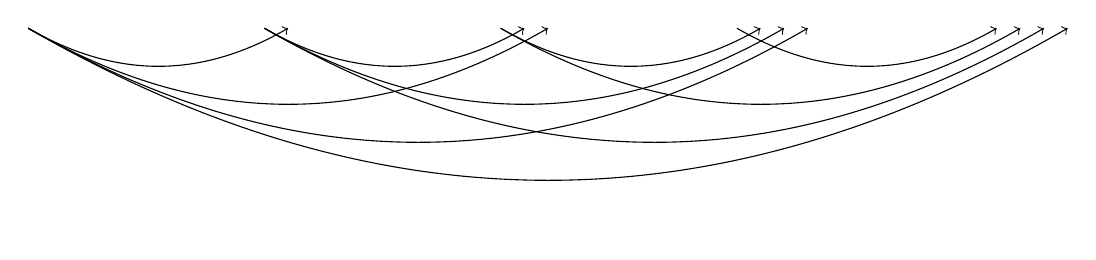
\begin{tikzpicture}
  \usetikzlibrary{3d}

  \def\scale{3}
  \def\netx{0}
  \def\nety{0}
  \def\netz{0}

  \def\coblue{blue!50!gray}
  \def\copurple{purple!50!gray}
  \def\coorange{orange!70!gray}
  \def\cogreen{green!50!gray}
  \def\copink{pink!50!gray}
  \def\comagenta{magenta!50!gray}
  \def\coyellow{yellow!50!white}
  \def\cored{red!50!white}

  \def\zoff{\netz+0.5*\scale}
  \def\yoff{\nety-0.5*\scale}
  \newcommand\denselink[2]{%
      \draw[->] (#1, \yoff, \zoff) to[bend right=30] (#2, \yoff, \zoff);
  }

  \convlayer{1*\scale}{1*\scale}{0.1*\scale}{Carte d'activation}{\copurple}{0.*\scale+\netx}{\nety}{\netz}{{}{}{}}
  \denselink{\netx+0*\scale}{\netx+1.1*\scale}
  \denselink{\netx+0*\scale}{\netx+2.2*\scale}
  \denselink{\netx+0*\scale}{\netx+3.3*\scale}
  \denselink{\netx+0*\scale}{\netx+4.4*\scale}

  \convlayer{1*\scale}{1*\scale}{0.1*\scale}{BN-ReLU-Conv}{\coblue}{\netx+1*\scale}{\nety}{\netz}{{}{}{}}
  \denselink{\netx+1*\scale}{\netx+2.1*\scale}
  \denselink{\netx+1*\scale}{\netx+3.2*\scale}
  \denselink{\netx+1*\scale}{\netx+4.3*\scale}

  \denselink{\netx+2*\scale}{\netx+3.1*\scale}
  \denselink{\netx+2*\scale}{\netx+4.2*\scale}

  \denselink{\netx+3*\scale}{\netx+4.1*\scale}

  \convlayer{1*\scale}{1*\scale}{0.1*\scale}{}{\copurple}{1.1*\scale+\netx}{\nety}{\netz}{{}{}{}}

  \convlayer{1*\scale}{1*\scale}{0.1*\scale}{BN-ReLU-Conv}{\copink}{\netx+2*\scale}{\nety}{\netz}{{}{}{}}
  \convlayer{1*\scale}{1*\scale}{0.1*\scale}{}{\coblue}{2.1*\scale+\netx}{\nety}{\netz}{{}{}{}}
  \convlayer{1*\scale}{1*\scale}{0.1*\scale}{}{\copurple}{2.2*\scale+\netx}{\nety}{\netz}{{}{}{}}

  \convlayer{1*\scale}{1*\scale}{0.1*\scale}{BN-ReLU-Conv}{\cored}{\netx+3*\scale}{\nety}{\netz}{{}{}{}}
  \convlayer{1*\scale}{1*\scale}{0.1*\scale}{}{\copink}{3.1*\scale+\netx}{\nety}{\netz}{{}{}{}}
  \convlayer{1*\scale}{1*\scale}{0.1*\scale}{}{\coblue}{3.2*\scale+\netx}{\nety}{\netz}{{}{}{}}
  \convlayer{1*\scale}{1*\scale}{0.1*\scale}{}{\copurple}{3.3*\scale+\netx}{\nety}{\netz}{{}{}{}}

  \convlayer{1*\scale}{1*\scale}{0.1*\scale}{BN-ReLU-Conv}{\comagenta}{\netx+4*\scale}{\nety}{\netz}{{}{}{}}
  \convlayer{1*\scale}{1*\scale}{0.1*\scale}{}{\cored}{4.1*\scale+\netx}{\nety}{\netz}{{}{}{}}
  \convlayer{1*\scale}{1*\scale}{0.1*\scale}{}{\copink}{4.2*\scale+\netx}{\nety}{\netz}{{}{}{}}
  \convlayer{1*\scale}{1*\scale}{0.1*\scale}{}{\coblue}{4.3*\scale+\netx}{\nety}{\netz}{{}{}{}}
  \convlayer{1*\scale}{1*\scale}{0.1*\scale}{}{\copurple}{4.4*\scale+\netx}{\nety}{\netz}{{}{}{}}

  \convlayer{1*\scale}{1*\scale}{0.2*\scale}{Transition}{\coyellow}{\netx+5.1*\scale}{\nety}{\netz}{{}{}{}}
  \convlayer{0.6*\scale}{0.6*\scale}{0.2*\scale}{Pooling}{\coorange}{\netx+5.7*\scale}{\nety}{\netz}{{}{}{}}
  \end{tikzpicture}
\end{document}

  }
  \caption[Bloc convolutif dense.]{Bloc convolutif dense~\cite{huang_densely_2017}.}
  \label{fig:denseblock}
  \end{minipage}
\end{figure}

Indépendamment, \citet{szegedy_going_2015} proposent le modèle GoogLeNet avec 22 couches. Cette architecture introduit notamment le module \emph{Inception} empilant plusieurs couches en parallèle, et plus seulement en profondeur. L'idée est de réaliser, pour une carte d'activation, l'extraction de caractéristiques à plusieurs niveaux de contexte en utilisant soit une convolution $1\times1$, c'est-à-dire une combinaison linéaire suivie d'une non-linéarité, soit un \emph{pooling}, soit des convolutions $3\times3$ ou $5\times5$. Cela permet de coupler des caractéristiques dotées de l'invariance aux translations locales (issues du sous-échantillonnage) et des caractéristiques qui ne le sont pas, ce qui permet de gérer une plus grande variété de cas. Le module \emph{Inception} est illustré dans la~\cref{fig:inception} tandis que la~\cref{fig:googlenet} détaille l'architecture complète du modèle GoogLeNet.
Compte-tenu de la profondeur du réseau (22 couches), ses auteurs proposent de faciliter l'optimisation des couches les plus basses en ajoutant un classifieur au niveau des représentations intermédiaires, après les modules \emph{Inception} (4a) et (4d). Cette approche profondément supervisée avait notamment déjà montré son efficacité pour lutter contre les problèmes de gradients évanescents~\cite{lee_deeply-supervised_2015}. Ce modèle obtient un taux d'erreur de seulement 6,4\% en reconnaissance d'objets à l'\gls{ILSVRC}.
L'architecture GoogleNet est améliorée~\cite{szegedy_rethinking_2016} par la suite en remplaçant les convolutions $5\times5$ du module \emph{Inception} par deux convolutions $3\times3$, comme proposé dans le modèle VGG~\cite{simonyan_very_2014} et en intégrant la \emph{Batch Normalization}~\cite{ioffe_batch_2015}.

\begin{figure}[t]
  \resizebox{\textwidth}{!}{
    \documentclass{standalone}
\usepackage[utf8]{inputenc}
\usepackage[T1]{fontenc}
\usepackage{tikz}
\usepackage{ifthen}
\usepackage{graphicx}
%%%%%%%%%%%%%%%%%%%%%%%%%%%%%%%%%%%%%%%%
%           Commandes perso            %
%%%%%%%%%%%%%%%%%%%%%%%%%%%%%%%%%%%%%%%%

%% Figures centrées, et en position 'here, top, bottom or page'
\newenvironment{figureth}{%
		\begin{figure}[htbp]
			\centering
	}{
		\end{figure}
		}


%% Tableaux centrés, et en position 'here, top, bottom or page'
\newenvironment{tableth}{%
		\begin{table}[htbp]
			\centering
			%\rowcolors{1}{coleurtableau}{coleurtableau}
	}{
		\end{table}
		}

%% Sous-figures centrées, en position 'top'
\newenvironment{subfigureth}[1]{%
	\begin{subfigure}[t]{#1}
	\centering
}{
	\end{subfigure}
}

\newcommand{\citationChap}[2]{%
	\epigraph{\og \textit{#1} \fg{}}{#2}
}

%% On commence par une page impaire quand on change le style de numérotation de pages
\let\oldpagenumbering\pagenumbering
\renewcommand{\pagenumbering}[1]{%
	\cleardoublepage
	\oldpagenumbering{#1}
}

%% Légende du dataset ISPRS
\newcommand\isprslegende{
Légende\,: \textcolor{Black}{blanc}\,: routes, \textcolor{Blue}{bleu}\,: bâtiments, \textcolor{Cerulean}{cyan}\,: végétation basse, \textcolor{OliveGreen}{vert}\,: arbres, \textcolor{Dandelion}{jaune}\,: véhicules, \textcolor{BrickRed}{rouge}\,: autre.
}

%% Dessiner des réseaux de neurones avec Tikz
\newcommand{\convlayer}[9]{%{h}{w}{d}{name}{color}{x}{y}{z}%{note w}{note h}{note d}
   \def\h{#1}
   \def\w{#2}
   \def\d{#3}
   \def\name{#4}
   \ifthenelse {\equal{#5} {}} {\def\col{white}} {\def\col{#5}}
   \def\x{#6}
   \ifthenelse {\equal{#7} {}} {\def\y{0}} {\def\y{#7}}
   \ifthenelse {\equal{#8} {}} {\def\z{0}} {\def\z{#8}}
   % ne faites pas ça chez vous !
   \ifthenelse {\equal{#9} {}} {\convlayercontinued{}{}{}} {\convlayercontinued#9}
}

\newcommand\convlayercontinued[3]{
   \def\notew{#1}
   \def\noteh{#2}
   \def\noted{#3}
   \coordinate (A) at (\x-\d/2,  \y-\h/2, \z-\w/2);
   \coordinate (B) at (\x-\d/2,  \y-\h/2, \z+\w/2);
   \coordinate (C) at (\x-\d/2,  \y+\h/2, \z+\w/2);
   \coordinate (D) at (\x-\d/2,  \y+\h/2, \z-\w/2);
   \coordinate (E) at (\x+\d/2,  \y-\h/2, \z-\w/2);
   \coordinate (F) at (\x+\d/2,  \y-\h/2, \z+\w/2);
   \coordinate (G) at (\x+\d/2,  \y+\h/2, \z+\w/2);
   \coordinate (H) at (\x+\d/2,  \y+\h/2, \z-\w/2);

    \draw [draw opacity=0.3, fill opacity=0.8, fill=\col!60!white] (A) -- (B) -- (C) -- (D) -- cycle;
    \draw [draw opacity=0.3, fill opacity=0.8, fill=\col!60!white] (A) -- (B) -- (F) -- (E) -- cycle;
    % Face haut
    %\draw [left color=\col!60!white, right color=\col!80!white, shading=axis, shading angle=180] (C) -- (D)  -- (H) -- (G) -- cycle;
    \draw [fill opacity=0.9, fill=\col!70!white] (C) -- node[rotate=45,above] {\small \name} (D) -- (H) -- (G) -- cycle;
    %\draw [fill opacity=0.9, fill=\col!70!white] (C) -- (D) -- node[above] {\small \name} (H) -- (G) -- cycle;
    % Face droite
    \draw [fill opacity=0.9, fill=\col!60!white] (E) -- node[pos=0.75,rotate=45,below] {\scriptsize \notew} (F) -- (G) --  (H) -- cycle;
    % Face avant
    %\draw [shading=axis, left color=\col!60!white, right color=\col!40!white, shading angle=-45] (B) -- node[above,rotate=90] {\scriptsize \noteh} (C) -- (G) -- (F) -- node[below] {\scriptsize \noted}  cycle;
    \draw [fill opacity=0.9, fill=\col!50!white] (B) -- node[above,rotate=90] {\scriptsize \noteh} (C) -- (G) -- (F) -- node[below] {\scriptsize \noted}  cycle;
}

\newcommand{\fclayer}[8]{%{h}{w}{name}{color}{x}{y}{z}
   \def\h{#1}
   \def\w{#2}
   \def\name{#3}
   \ifthenelse {\equal{#4} {}} {\def\col{white}} {\def\col{#4}}
   \def\x{#5}
   \def\y{#6}
   \def\z{#7}
   \def\note{#8}
   \coordinate (A) at (\x-\w/2,  \y-\h/2, \z);
   \coordinate (B) at (\x+\w/2,  \y-\h/2, \z);
   \coordinate (C) at (\x+\w/2,  \y+\h/2, \z);
   \coordinate (D) at (\x-\w/2,  \y+\h/2, \z);

   \pgfmathparse{4*\w}\let\boxwidth\pgfmathresult
    \draw [fill=\col] (A) -- node[below,text width=\boxwidth cm,align=center] {\scriptsize \note} (B) -- (C) -- (D) -- cycle;

    \node (N) at ($(A)!0.5!(B)+(0,-1,0)$) {\name};
}

\newcommand{\alexnet}[4]{%{scale}{x}{y}{z}
  \def\scale{#1}
  \def\alexx{#2}
  \def\alexy{#3}
  \def\alexz{#4}


  \def\coblue{blue!50!white}
  \def\fcgrey{gray!50!white}

  \convlayer{1.3*\scale}{1.3*\scale}{0.02*\scale}{Image}{\coblue}{\alexx}{\alexy}{\alexz}{{227}{227}{3}}
  \convlayer{1.1*\scale}{1.1*\scale}{0.08*\scale}{Conv1}{\coblue}{\alexx+0.7*\scale}{\alexy}{\alexz}{{55}{55}{96}}
  \convlayer{0.7*\scale}{0.7*\scale}{0.5*\scale}{Conv2}{\coblue}{\alexx+1.5*\scale}{\alexy}{\alexz}{{27}{27}{256}}
  \convlayer{0.5*\scale}{0.5*\scale}{0.8*\scale}{Conv3}{\coblue}{\alexx+2.6*\scale}{\alexy}{\alexz}{{13}{13}{384}}
  \convlayer{0.5*\scale}{0.5*\scale}{0.8*\scale}{Conv4}{\coblue}{\alexx+3.8*\scale}{\alexy}{\alexz}{{13}{13}{384}}
  \convlayer{0.5*\scale}{0.5*\scale}{0.5*\scale}{Conv5}{\coblue}{\alexx+4.8*\scale}{\alexy}{\alexz}{{13}{13}{256}}
  \fclayer{\scale}{0.1*\scale}{FC1}{\fcgrey}{\alexx+5.4*\scale}{\alexy}{\alexz}{4096}
  \fclayer{\scale}{0.1*\scale}{FC2}{\fcgrey}{\alexx+5.7*\scale}{\alexy}{\alexz}{4096}
  \fclayer{\scale}{0.1*\scale}{FC3}{\fcgrey}{\alexx+6.0*\scale}{\alexy}{\alexz}{1000}
}

\newcommand{\imagelayer}[7]{%{width}{x}{y}{z}{path}{text_up}{text_down}
    \pgfmathparse{#1}\let\w\pgfmathresult
    \begin{scope}[canvas is yz plane at x=#2]
     \node[transform shape] (source) at (#3, #4) {\includegraphics[angle=-90,width=\w cm]{#5}};
    \end{scope}
     \node [transform shape, rotate=45, above] at (source.east) {#6};
     \node [transform shape, rotate=45, below] at (source.west) {\scriptsize{#7}};
}

\def\fourier{\mathcal{F}}

\newcommand{\lightspectrum}{%
\pgfplotsset{
    % this *defines* a custom colormap ...
    colormap={slategraywhite}{color(0cm)=(red); color(1cm)=(red); color(2cm)=(red); color(3cm)=(red); color(4cm)=(orange); color(5cm)=(yellow); color(6cm)=(green); color(7cm)=(blue); color(8cm)=(blue); color(9cm)=(purple); color(10cm)=(purple); color(12cm)=(black)}
}
\node at (1.5, 2.7) {\small 1mm};
\node at (4, 3) {Infrarouge};
\node at (7.75, 2.7) {\small 800nm};
\node at (9, 3) {Visible};
\node at (10.5, 2.7) {\small 400nm};
\node at (12, 3) {Ultraviolet};
\node at (13.5, 2.7) {\small 10nm};
\draw[->] (1, 2.5) -- (14, 2.5);
\begin{axis}[hide axis,width=16cm,height=4cm,colormap name=slategraywhite]
\addplot[domain=20:1000,samples=1500,ultra thick, point meta=x*x,mesh]{sin(x*x/80)};
\end{axis}
}

% Union généralisée
\newcommand{\wbigcup}{\mathop{\bigcup}\displaylimits}

\newcommand{\res}[2]{#1 {\footnotesize $\pm$ #2}}
\newcommand{\bres}[2]{\textbf{#1} {\footnotesize $\pm$ #2}}
\newcommand{\bbres}[2]{\res{\textit{#1}}{#2}}

\newcommand{\drawkernel}[9]{
\begin{tikzpicture}
	\draw[step=1cm,gray!50!white,very thin] (0,0) grid (3,3);
	\kernelnode{0.5}{0.5}{#1};
	\kernelnode{0.5}{1.5}{#2};
	\kernelnode{0.5}{2.5}{#3};
	\kernelnode{1.5}{0.5}{#4};
	\kernelnode{1.5}{1.5}{#5};
	\kernelnode{1.5}{2.5}{#6};
	\kernelnode{2.5}{0.5}{#7};
	\kernelnode{2.5}{1.5}{#8};
	\kernelnode{2.5}{2.5}{#9};
\end{tikzpicture}
}

\newcommand{\kernelnode}[3]{%{x}{y}{value}
	\ifthenelse{\equal{#3}{0}}{
		\def\kcolor{gray}
	}{
		\def\kcolor{black}
	}
	\node[\kcolor] at (#1, #2) {#3};
}

\newcommand{\chapsummary}[1]{
\section*{Résumé du chapitre :}
\parbox{0.9\linewidth}{
\setlength{\parindent}{4ex}
#1}
}

\newcommand{\eqname}[1]{\tag*{\small (#1)}}


\begin{document}
  \begin{tikzpicture}
  \usetikzlibrary{calc}
  \usetikzlibrary{3d}

  \def\scale{4}
  \def\vggx{0}
  \def\vggy{0}
  \def\vggz{0}

  \def\coblue{blue!50!gray}
  \def\cored{red!50!gray}
  \def\coorange{orange!70!gray}
  \def\cogreen{green!50!gray}
  \def\copurple{purple!50!white}

  \imagelayer{1.3*\scale}{-0.3*\scale+\vggx}{\vggy}{\vggz}{nobu}{Image}{$224\times224\times3$}
  \convlayer{1.3*\scale}{1.3*\scale}{0.02*\scale}{Image}{\coblue}{0.2*\scale+\vggx}{\vggy}{\vggz}{{224}{}{3}}
  \convlayer{1*\scale}{1*\scale}{0.04*\scale}{Conv1}{\coblue}{\vggx+0.6*\scale}{\vggy}{\vggz}{{112}{112}{64}}
  \convlayer{0.8*\scale}{0.8*\scale}{0.04*\scale}{Pool1}{\coorange}{\vggx+1*\scale}{\vggy}{\vggz}{{56}{56}{}}

  \foreach \ratio [count=\ni] in {1.4,1.5,1.6,1.7,1.8,1.9}{
  \convlayer{0.8*\scale}{0.8*\scale}{0.04*\scale}{}{\coblue}{\vggx+\ratio*\scale}{\vggy}{\vggz}{{}{}{64}}
  \ifnum\ni=1%
      \draw (\vggx+\ratio*\scale-0.3*\scale, \vggy+0.5*\scale) edge[dashed,thick,->,in=90,out=90,looseness=2] (\vggx+\ratio*\scale, \vggy+0.4*\scale);
  \else%
      \draw (\vggx+\ratio*\scale-0.1*\scale+0.035*\scale, \vggy+0.4*\scale) edge[thick,->,in=90,out=90,looseness=10] (\vggx+\ratio*\scale, \vggy+0.4*\scale);
  \fi%
  }


  \foreach \ratio [count=\ni] in {2.2,2.35,2.5,2.65,2.8,2.95,3.10,3.25}{
  \convlayer{0.6*\scale}{0.6*\scale}{0.08*\scale}{}{\coblue}{\vggx+\ratio*\scale}{\vggy}{\vggz}{{}{}{128}}
  \ifnum\ni=1%
      \draw (\vggx+\ratio*\scale-0.2*\scale, \vggy+0.5*\scale) edge[dashed,looseness=2,thick,->,in=90,out=90] (\vggx+\ratio*\scale, \vggy+0.3*\scale);%
  \else%
      \draw (\vggx+\ratio*\scale-0.15*\scale+0.035*\scale, \vggy+0.3*\scale) edge[looseness=5,thick,->,in=90,out=90] (\vggx+\ratio*\scale, \vggy+0.3*\scale);%
  \fi%
  }

  \foreach \ratio [count=\ni] in {3.5,3.7,3.9,4.1,4.3,4.5,4.7,4.9,5.1,5.3,5.5,5.7}{
  \convlayer{0.4*\scale}{0.4*\scale}{0.12*\scale}{}{\coblue}{\vggx+\ratio*\scale}{\vggy}{\vggz}{{}{}{256}}
  \ifnum\ni=1%
      \draw (\vggx+\ratio*\scale-0.2*\scale, \vggy+0.3*\scale) edge[dashed,thick,looseness=1.5,->,in=90,out=90] (\vggx+\ratio*\scale, \vggy+0.2*\scale);
  \else%
      \draw (\vggx+\ratio*\scale-0.2*\scale+0.035*\scale, \vggy+0.2*\scale) edge[thick,looseness=2,->,in=90,out=90] (\vggx+\ratio*\scale, \vggy+0.2*\scale);
  \fi%
  }

  \foreach \ratio [count=\ni] in {6,6.3,6.6,6.9,7.2,7.5,7.8}{
  \convlayer{0.3*\scale}{0.3*\scale}{0.2*\scale}{}{\coblue}{\vggx+\ratio*\scale}{\vggy}{\vggz}{{}{}{512}}
  \ifnum\ni=1%
      \draw (\vggx+\ratio*\scale-0.3*\scale+0.05*\scale, \vggy+0.225*\scale) edge[dashed,thick,->,in=90,out=90,looseness=1.25] (\vggx+\ratio*\scale, \vggy+0.15*\scale);
  \else%
      \draw (\vggx+\ratio*\scale-0.3*\scale+0.05*\scale, \vggy+0.15*\scale) edge[thick,->,in=90,out=90,looseness=1.5] (\vggx+\ratio*\scale, \vggy+0.15*\scale);
  \fi%
  }

  \node at (\vggx+8.3*\scale, \vggy+0.2*\scale) {Avg. pool};
  \convlayer{0.1*\scale}{0.1*\scale}{0.6*\scale}{}{\coorange}{\vggx+8.3*\scale}{\vggy}{\vggz}{{}{}{$1\times1\times1024$}}
  \fclayer{\scale}{0.1*\scale}{FC}{\copurple}{\vggx+8.7*\scale}{\vggy}{\vggz}{1000}
  \node (out) at (\vggx+9.1*\scale,\vggy) {\Large ``Chat''};
  \draw[->] (\vggx+8.75*\scale,\vggy) -- (out.west);

  \end{tikzpicture}
\end{document}

  }
  \caption[Architecture ResNet-34.]{Architecture ResNet-34~\cite{he_deep_2016}.}
  \label{fig:resnet}
\end{figure}

En 2015, \citet{he_deep_2016} parviennent à obtenir un taux d'erreur de seulement 3,5\% en reconnaissance d'objet durant \gls{ILSVRC}. Leur approche consiste en un réseau très profond comprenant plus de 100 couches convolutives. L'optimisation est rendue possible d'une part grâce à la \emph{Batch Normalization}, mais surtout grâce à l'apprentissage par résidu. L'idée est de briser la structure purement séquentielle des réseaux à propagation avant en ajoutant des connexions permettant de court-circuiter la couche suivante. Ces connexions, dites résiduelles, correspondent à une simple opération identité et permettent alors aux activations et au gradient de parcourir l'ensemble du réseau sans subir d’évanescence ou d'explosion dues à la règle de la dérivation en chaîne. Plutôt que de chercher à approcher $f\,: x \rightarrow f(x)$, le bloc résiduel va approcher $\hat{f}\,: x \rightarrow f(x) - x$, plus simple car d'amplitude a priori plus faible. Le bloc de convolution résiduel est illustré dans la~\cref{fig:residual} et un exemple de modèle dit \emph{ResNet} à 34 couches est détaillé dans la~\cref{fig:resnet}. L'introduction de l'apprentissage par résidu change en partie le paradigme utilisée jusqu'alors pour la conception des \gls{CNN}. Le bloc de base constitutif du réseau passe ainsi au bloc résiduel.
Les ResNet possèdent beaucoup de couches mais comparativement peu de paramètres, car seule la dernière couche est entièrement connectée. Comme nous l'avons vu, les couches entièrement connectées concentrent en général la majorité des poids des \gls{CNN} et sont également les plus sensibles au surapprentissage, nécessitant l'intégration de régularisations comme le \emph{Dropout}~\cite{srivastava_dropout_2014}. ResNet ne contient quasiment que des convolutions $3\times3$, à l'exception de la première convolution $7\times7$ qui permet de réduire brutalement les dimensions spatiales de l'image. Il est intéressant de constater que la réduction de dimension finale avant la couche entièrement connectée se fait à l'aide d'un sous-échantillonnage adaptatif. Ainsi, peu importe la taille de l'image de l'entrée\,: le sous-échantillonnage moyennera les activations pour produire le vecteur de caractéristiques de taille attendue par la couche entièrement connectée. Cependant, il faut noter que le nombre élevé d'activations et de gradients intermédiaires à calculer rend les ResNet coûteux en mémoire et peu pratiques sur de grandes images. L'architecture \emph{Inception} sera également améliorée par des connexions résiduelles~\cite{szegedy_inception-v4_2017}.


\begin{figure}[t]
  \resizebox{\textwidth}{!}{
    \documentclass{standalone}
\usepackage[utf8]{inputenc}
\usepackage[T1]{fontenc}
\usepackage{tikz}
\usepackage{ifthen}
\usepackage{graphicx}
%%%%%%%%%%%%%%%%%%%%%%%%%%%%%%%%%%%%%%%%
%           Commandes perso            %
%%%%%%%%%%%%%%%%%%%%%%%%%%%%%%%%%%%%%%%%

%% Figures centrées, et en position 'here, top, bottom or page'
\newenvironment{figureth}{%
		\begin{figure}[htbp]
			\centering
	}{
		\end{figure}
		}


%% Tableaux centrés, et en position 'here, top, bottom or page'
\newenvironment{tableth}{%
		\begin{table}[htbp]
			\centering
			%\rowcolors{1}{coleurtableau}{coleurtableau}
	}{
		\end{table}
		}

%% Sous-figures centrées, en position 'top'
\newenvironment{subfigureth}[1]{%
	\begin{subfigure}[t]{#1}
	\centering
}{
	\end{subfigure}
}

\newcommand{\citationChap}[2]{%
	\epigraph{\og \textit{#1} \fg{}}{#2}
}

%% On commence par une page impaire quand on change le style de numérotation de pages
\let\oldpagenumbering\pagenumbering
\renewcommand{\pagenumbering}[1]{%
	\cleardoublepage
	\oldpagenumbering{#1}
}

%% Légende du dataset ISPRS
\newcommand\isprslegende{
Légende\,: \textcolor{Black}{blanc}\,: routes, \textcolor{Blue}{bleu}\,: bâtiments, \textcolor{Cerulean}{cyan}\,: végétation basse, \textcolor{OliveGreen}{vert}\,: arbres, \textcolor{Dandelion}{jaune}\,: véhicules, \textcolor{BrickRed}{rouge}\,: autre.
}

%% Dessiner des réseaux de neurones avec Tikz
\newcommand{\convlayer}[9]{%{h}{w}{d}{name}{color}{x}{y}{z}%{note w}{note h}{note d}
   \def\h{#1}
   \def\w{#2}
   \def\d{#3}
   \def\name{#4}
   \ifthenelse {\equal{#5} {}} {\def\col{white}} {\def\col{#5}}
   \def\x{#6}
   \ifthenelse {\equal{#7} {}} {\def\y{0}} {\def\y{#7}}
   \ifthenelse {\equal{#8} {}} {\def\z{0}} {\def\z{#8}}
   % ne faites pas ça chez vous !
   \ifthenelse {\equal{#9} {}} {\convlayercontinued{}{}{}} {\convlayercontinued#9}
}

\newcommand\convlayercontinued[3]{
   \def\notew{#1}
   \def\noteh{#2}
   \def\noted{#3}
   \coordinate (A) at (\x-\d/2,  \y-\h/2, \z-\w/2);
   \coordinate (B) at (\x-\d/2,  \y-\h/2, \z+\w/2);
   \coordinate (C) at (\x-\d/2,  \y+\h/2, \z+\w/2);
   \coordinate (D) at (\x-\d/2,  \y+\h/2, \z-\w/2);
   \coordinate (E) at (\x+\d/2,  \y-\h/2, \z-\w/2);
   \coordinate (F) at (\x+\d/2,  \y-\h/2, \z+\w/2);
   \coordinate (G) at (\x+\d/2,  \y+\h/2, \z+\w/2);
   \coordinate (H) at (\x+\d/2,  \y+\h/2, \z-\w/2);

    \draw [draw opacity=0.3, fill opacity=0.8, fill=\col!60!white] (A) -- (B) -- (C) -- (D) -- cycle;
    \draw [draw opacity=0.3, fill opacity=0.8, fill=\col!60!white] (A) -- (B) -- (F) -- (E) -- cycle;
    % Face haut
    %\draw [left color=\col!60!white, right color=\col!80!white, shading=axis, shading angle=180] (C) -- (D)  -- (H) -- (G) -- cycle;
    \draw [fill opacity=0.9, fill=\col!70!white] (C) -- node[rotate=45,above] {\small \name} (D) -- (H) -- (G) -- cycle;
    %\draw [fill opacity=0.9, fill=\col!70!white] (C) -- (D) -- node[above] {\small \name} (H) -- (G) -- cycle;
    % Face droite
    \draw [fill opacity=0.9, fill=\col!60!white] (E) -- node[pos=0.75,rotate=45,below] {\scriptsize \notew} (F) -- (G) --  (H) -- cycle;
    % Face avant
    %\draw [shading=axis, left color=\col!60!white, right color=\col!40!white, shading angle=-45] (B) -- node[above,rotate=90] {\scriptsize \noteh} (C) -- (G) -- (F) -- node[below] {\scriptsize \noted}  cycle;
    \draw [fill opacity=0.9, fill=\col!50!white] (B) -- node[above,rotate=90] {\scriptsize \noteh} (C) -- (G) -- (F) -- node[below] {\scriptsize \noted}  cycle;
}

\newcommand{\fclayer}[8]{%{h}{w}{name}{color}{x}{y}{z}
   \def\h{#1}
   \def\w{#2}
   \def\name{#3}
   \ifthenelse {\equal{#4} {}} {\def\col{white}} {\def\col{#4}}
   \def\x{#5}
   \def\y{#6}
   \def\z{#7}
   \def\note{#8}
   \coordinate (A) at (\x-\w/2,  \y-\h/2, \z);
   \coordinate (B) at (\x+\w/2,  \y-\h/2, \z);
   \coordinate (C) at (\x+\w/2,  \y+\h/2, \z);
   \coordinate (D) at (\x-\w/2,  \y+\h/2, \z);

   \pgfmathparse{4*\w}\let\boxwidth\pgfmathresult
    \draw [fill=\col] (A) -- node[below,text width=\boxwidth cm,align=center] {\scriptsize \note} (B) -- (C) -- (D) -- cycle;

    \node (N) at ($(A)!0.5!(B)+(0,-1,0)$) {\name};
}

\newcommand{\alexnet}[4]{%{scale}{x}{y}{z}
  \def\scale{#1}
  \def\alexx{#2}
  \def\alexy{#3}
  \def\alexz{#4}


  \def\coblue{blue!50!white}
  \def\fcgrey{gray!50!white}

  \convlayer{1.3*\scale}{1.3*\scale}{0.02*\scale}{Image}{\coblue}{\alexx}{\alexy}{\alexz}{{227}{227}{3}}
  \convlayer{1.1*\scale}{1.1*\scale}{0.08*\scale}{Conv1}{\coblue}{\alexx+0.7*\scale}{\alexy}{\alexz}{{55}{55}{96}}
  \convlayer{0.7*\scale}{0.7*\scale}{0.5*\scale}{Conv2}{\coblue}{\alexx+1.5*\scale}{\alexy}{\alexz}{{27}{27}{256}}
  \convlayer{0.5*\scale}{0.5*\scale}{0.8*\scale}{Conv3}{\coblue}{\alexx+2.6*\scale}{\alexy}{\alexz}{{13}{13}{384}}
  \convlayer{0.5*\scale}{0.5*\scale}{0.8*\scale}{Conv4}{\coblue}{\alexx+3.8*\scale}{\alexy}{\alexz}{{13}{13}{384}}
  \convlayer{0.5*\scale}{0.5*\scale}{0.5*\scale}{Conv5}{\coblue}{\alexx+4.8*\scale}{\alexy}{\alexz}{{13}{13}{256}}
  \fclayer{\scale}{0.1*\scale}{FC1}{\fcgrey}{\alexx+5.4*\scale}{\alexy}{\alexz}{4096}
  \fclayer{\scale}{0.1*\scale}{FC2}{\fcgrey}{\alexx+5.7*\scale}{\alexy}{\alexz}{4096}
  \fclayer{\scale}{0.1*\scale}{FC3}{\fcgrey}{\alexx+6.0*\scale}{\alexy}{\alexz}{1000}
}

\newcommand{\imagelayer}[7]{%{width}{x}{y}{z}{path}{text_up}{text_down}
    \pgfmathparse{#1}\let\w\pgfmathresult
    \begin{scope}[canvas is yz plane at x=#2]
     \node[transform shape] (source) at (#3, #4) {\includegraphics[angle=-90,width=\w cm]{#5}};
    \end{scope}
     \node [transform shape, rotate=45, above] at (source.east) {#6};
     \node [transform shape, rotate=45, below] at (source.west) {\scriptsize{#7}};
}

\def\fourier{\mathcal{F}}

\newcommand{\lightspectrum}{%
\pgfplotsset{
    % this *defines* a custom colormap ...
    colormap={slategraywhite}{color(0cm)=(red); color(1cm)=(red); color(2cm)=(red); color(3cm)=(red); color(4cm)=(orange); color(5cm)=(yellow); color(6cm)=(green); color(7cm)=(blue); color(8cm)=(blue); color(9cm)=(purple); color(10cm)=(purple); color(12cm)=(black)}
}
\node at (1.5, 2.7) {\small 1mm};
\node at (4, 3) {Infrarouge};
\node at (7.75, 2.7) {\small 800nm};
\node at (9, 3) {Visible};
\node at (10.5, 2.7) {\small 400nm};
\node at (12, 3) {Ultraviolet};
\node at (13.5, 2.7) {\small 10nm};
\draw[->] (1, 2.5) -- (14, 2.5);
\begin{axis}[hide axis,width=16cm,height=4cm,colormap name=slategraywhite]
\addplot[domain=20:1000,samples=1500,ultra thick, point meta=x*x,mesh]{sin(x*x/80)};
\end{axis}
}

% Union généralisée
\newcommand{\wbigcup}{\mathop{\bigcup}\displaylimits}

\newcommand{\res}[2]{#1 {\footnotesize $\pm$ #2}}
\newcommand{\bres}[2]{\textbf{#1} {\footnotesize $\pm$ #2}}
\newcommand{\bbres}[2]{\res{\textit{#1}}{#2}}

\newcommand{\drawkernel}[9]{
\begin{tikzpicture}
	\draw[step=1cm,gray!50!white,very thin] (0,0) grid (3,3);
	\kernelnode{0.5}{0.5}{#1};
	\kernelnode{0.5}{1.5}{#2};
	\kernelnode{0.5}{2.5}{#3};
	\kernelnode{1.5}{0.5}{#4};
	\kernelnode{1.5}{1.5}{#5};
	\kernelnode{1.5}{2.5}{#6};
	\kernelnode{2.5}{0.5}{#7};
	\kernelnode{2.5}{1.5}{#8};
	\kernelnode{2.5}{2.5}{#9};
\end{tikzpicture}
}

\newcommand{\kernelnode}[3]{%{x}{y}{value}
	\ifthenelse{\equal{#3}{0}}{
		\def\kcolor{gray}
	}{
		\def\kcolor{black}
	}
	\node[\kcolor] at (#1, #2) {#3};
}

\newcommand{\chapsummary}[1]{
\section*{Résumé du chapitre :}
\parbox{0.9\linewidth}{
\setlength{\parindent}{4ex}
#1}
}

\newcommand{\eqname}[1]{\tag*{\small (#1)}}


\begin{document}
  \begin{tikzpicture}
  \usetikzlibrary{calc}
  \usetikzlibrary{3d}

  \def\scale{4}
  \def\vggx{0}
  \def\vggy{0}
  \def\vggz{0}

  \def\coblue{blue!50!gray}
  \def\cored{red!50!gray}
  \def\coorange{orange!70!gray}
  \def\cogreen{green!50!gray}
  \def\copurple{purple!50!white}

  \imagelayer{1.3*\scale}{-0.3*\scale+\vggx}{\vggy}{\vggz}{nobu}{Image}{$224\times224\times3$}
  \convlayer{1.3*\scale}{1.3*\scale}{0.01*\scale}{Image}{\coblue}{0.2*\scale+\vggx}{\vggy}{\vggz}{{224}{}{3}}
  \convlayer{1*\scale}{1*\scale}{0.02*\scale}{Conv1}{\coblue}{\vggx+0.6*\scale}{\vggy}{\vggz}{{112}{112}{64}}
  \convlayer{0.8*\scale}{0.8*\scale}{0.02*\scale}{Pool1}{\coorange}{\vggx+1*\scale}{\vggy}{\vggz}{{56}{56}{}}

  \foreach \ratio [count=\ni] in {1.4,1.44,...,2.28}{
  \convlayer{0.8*\scale}{0.8*\scale}{0.04*\scale}{}{\cored}{\vggx+\ratio*\scale}{\vggy}{\vggz}{{}{}{}}
  }

  \convlayer{0.6*\scale}{0.6*\scale}{0.04*\scale}{Transition}{\coblue}{\vggx+2.5*\scale}{\vggy}{\vggz}{{}{}{}}

  \foreach \ratio [count=\ni] in {2.75,2.79,...,3.71}{
  \convlayer{0.6*\scale}{0.6*\scale}{0.04*\scale}{}{\cored}{\vggx+\ratio*\scale}{\vggy}{\vggz}{{}{}{}}
  }

  \convlayer{0.4*\scale}{0.4*\scale}{0.04*\scale}{Transition}{\coblue}{\vggx+4*\scale}{\vggy}{\vggz}{{}{}{}}

  \foreach \ratio [count=\ni] in {4.2,4.24,...,6.04}{
  \convlayer{0.4*\scale}{0.4*\scale}{0.04*\scale}{}{\cored}{\vggx+\ratio*\scale}{\vggy}{\vggz}{{}{}{}}
  }

  \convlayer{0.2*\scale}{0.2*\scale}{0.04*\scale}{Transition}{\coblue}{\vggx+6.25*\scale}{\vggy}{\vggz}{{}{}{}}

  \foreach \ratio [count=\ni] in {6.5,6.54,...,7.28}{
  \convlayer{0.2*\scale}{0.2*\scale}{0.04*\scale}{}{\cored}{\vggx+\ratio*\scale}{\vggy}{\vggz}{{}{}{}}
  }

  \node at (\vggx+8.3*\scale, \vggy+0.2*\scale) {Avg. pool};
  \convlayer{0.1*\scale}{0.1*\scale}{0.6*\scale}{}{\coorange}{\vggx+8.3*\scale}{\vggy}{\vggz}{{}{}{$1\times1\times1024$}}
  \fclayer{\scale}{0.1*\scale}{FC}{\copurple}{\vggx+8.7*\scale}{\vggy}{\vggz}{1000}
  \node (out) at (\vggx+9.1*\scale,\vggy) {\Large ``Chat''};
  \draw[->] (\vggx+8.75*\scale,\vggy) -- (out.west);

  \end{tikzpicture}
\end{document}

  }
  \caption[Architecture DenseNet-121.]{Architecture DenseNet-121~\cite{huang_densely_2017}.}
  \label{fig:densenet}
\end{figure}


L'utilisation de cartes d'activation intermédiaires et leur propagation aux couches supérieures permet une meilleure classification en prenant en compte plusieurs niveaux d'abstraction. En outre, plusieurs travaux suggèrent que ces approches permettent en pratique de combiner plusieurs modèles en un seul, les activations étant en mesure de suivre plusieurs chemins dans la topologie du réseau~\cite{veit_residual_2016,huang_deep_2016}. Toutefois, les connexions résiduelles ne permettent que d'accéder aux activations de la couche précédente. \citet{huang_densely_2017} ont donc proposé une architecture dite \emph{DenseNet} comportant des connexions denses, construisant un modèle au sein duquel toutes les cartes d'activation issues des couches inférieures sont transmises à toutes les couches supérieures. Pour éviter l'explosion du nombre de paramètres et d'activations, le modèle est divisé en plusieurs blocs denses, comme illustré dans la~\cref{fig:densenet}. Chaque bloc se détaille comme illustré dans la~\cref{fig:denseblock}. La présence des connexions denses permet au gradient de se propager immédiatement des couches supérieures aux couches inférieures, appliquant ainsi une forme implicite de supervision profonde~\cite{lee_deeply-supervised_2015}. Entre deux blocs, une couche convolutive de transition est appliquée pour réduire le nombre de plans et est suivie d'un \emph{max-pooling} pour réduire les dimensions spatiales. Cette architecture obtient comparativement de meilleurs résultats que les modèles ResNet sur la base de validation de l'\gls{ILSVRC} 2012. Mais, à l'instar des ResNet, si le nombre de paramètres des architectures DenseNet est faible, ces modifications sont coûteuses en espace mémoire nécessaire pour stocker les activations et gradients intermédiaires.

Enfin, \citet{chollet_xception_2017} introduit les convolutions séparables en profondeur ou \emph{depthwise separable convolutions}. Celles-ci opèrent un filtre par plan du tenseur d'activation et sont recombinées pixel à pixel par une convolution point à point de noyau $1\times1$. Ainsi, il s'agit d'un cas spécifique de la convolution usuelle dans laquelle chaque plan du tenseur est filtré par un et un seul noyau de convolution, comme illustré dans la~\cref{fig:depthwise}. Ces convolutions sont introduites pour remplacer le module \emph{Inception} dans l'architecture éponyme et en ont amélioré les performances sur les jeux de données ImageNet et JFT, interne à Google. Un avantage notable de ces convolutions est de nécessiter moins de paramètres que la convolution classique. En effet, une convolution $k_1 \times k_2$ opérant sur $N_{in}$ cartes d'activations produisant $N_{out}$ cartes d'activations nécessite $k_1 \times k_2 \times N_{in} \times N_{out}$ paramètres. La convolution séparable en profondeur nécessite $N_{in} \times N_{in} \times k_1 \times k_2$ paramètres pour la première phase puis $N_{in} \times N_{out}$ pour la seconde, soit un total de $N_{in} \times (N_{in} \cdot k_1 \cdot k_2 + N_{out})$, ce qui est avantageux quand $N_{out} \ge N_{in}$, ce qui est le cas le plus courant. Ces convolutions séparables sont ainsi efficaces à calculer et de fait populaires pour des applications embarquées en temps réel~\cite{howard_mobilenets_2017}.

Bien que ces succès soient encourageants, il est nécessaire de rappeler que la classification d'images ne donne aucune information particulière de localisation, seulement une information binaire de présence d'un objet dans une image. Les premières approches de localisation ont cherché à calculer des caractéristiques denses sur l'image, associées à des cascades multi-échelles de classifieurs pour détecter des objets dans chaque sous-région de l'image. C'est l'approche utilisée par les descripteurs \gls{SIFT}~\cite{lowe_object_1999}, les pseudo-Haar de la méthode de~\citet{viola_robust_2001} ou encore des \gls{HOG}~\cite{dalal_histograms_2005}. Des approches à base de réseaux profonds pour la détection d'objet à partir de classification de sous-régions de l'image ont rapidement vu le jour~\cite{girshick_rich_2014,liu_ssd_2016,girshick_region-based_2016}, supplantant les techniques traditionnelles de localisation à partir d'extraction de fenêtres candidates~\cite{gu_recognition_2009,uijlings_selective_2013}. Le principe reste néanmoins identique. Il s'agit de réaliser une extraction dense de caractéristiques afin d'identifier les régions de l'image susceptibles de contenir un objet d'intérêt. Cependant, ces approches ne répondent pas exactement au problème décrit par Papert en 1966. La question n'est pas uniquement de pouvoir identifier des objets, mais aussi d'en estimer la forme et de les séparer du fond, comme illustré dans la~\cref{fig:classif_vs_seg}. Cette tâche est dite de \emph{segmentation sémantique} et correspond à l'association d'une classe d'intérêt non pas à chaque image, mais à chaque pixel de celle-ci.

Plusieurs jeux de données ont été introduits dans la communauté de la vision par ordinateur afin d'évaluer les techniques de segmentation sémantique, notamment sur des scènes de la vie quotidienne, comme PASCAL VOC~\cite{everingham_pascal_2014}, Microsoft COCO~\cite{lin_microsoft_2014} et également sur des scènes de conduite autonome avec des bases de données telles que CamVid~\cite{brostow_semantic_2009}, Cityscapes~\cite{cordts_cityscapes_2016} ou encore Mapillary Vistas~\cite{neuhold_mapillary_2017}. Les premières approches de segmentation sémantique ont réalisé des classifications à partir de caractéristiques denses calculées sur l'ensemble de l'image, regroupées \emph{a posteriori} par régions homogènes~\cite{shotton_semantic_2008,shotton_real-time_2011}. Les réseaux convolutifs profonds ont également été mis à contribution, en exploitant leur nature convolutive pour réaliser une classification sur chaque pixel de l'image~\cite{grangier_deep_2009,ciresan_deep_2012} ou pour chaque région~\cite{farabet_towards_2013,sermanet_overfeat_2013}. En effet, les cartes de caractéristiques issues des couches convolutives conservent la structure spatiale de l'image. Il est possible de faire correspondre chaque caractéristique à un ou plusieurs pixels de l'image initiale. Cette extraction de caractéristiques dense se prête particulièrement aux problématiques de localisation d'objet et a été rapidement adoptée par la communauté~\cite{zou_generic_2014}. Nous détaillerons un peu plus en détail certaines de ces approches dans le~\cref{chap:cartographie}. Dans la suite de cette partie, nous nous intéressons plus particulièrement aux réseaux profonds entièrement convolutifs, destinés à la classification dense pixel à pixel. En effet, ceux-ci sont une évolution naturelle des approches d'extraction dense de caractéristique, permettant un apprentissage de bout en bout pour la segmentation sémantique.

\subsection{Approches entièrement convolutives}

\begin{figure}
  \resizebox{\textwidth}{!}{%
  \documentclass{standalone}
\usepackage[utf8]{inputenc}
\usepackage[T1]{fontenc}
\usepackage{tikz}
\usepackage{ifthen}
%%%%%%%%%%%%%%%%%%%%%%%%%%%%%%%%%%%%%%%%
%           Commandes perso            %
%%%%%%%%%%%%%%%%%%%%%%%%%%%%%%%%%%%%%%%%

%% Figures centrées, et en position 'here, top, bottom or page'
\newenvironment{figureth}{%
		\begin{figure}[htbp]
			\centering
	}{
		\end{figure}
		}


%% Tableaux centrés, et en position 'here, top, bottom or page'
\newenvironment{tableth}{%
		\begin{table}[htbp]
			\centering
			%\rowcolors{1}{coleurtableau}{coleurtableau}
	}{
		\end{table}
		}

%% Sous-figures centrées, en position 'top'
\newenvironment{subfigureth}[1]{%
	\begin{subfigure}[t]{#1}
	\centering
}{
	\end{subfigure}
}

\newcommand{\citationChap}[2]{%
	\epigraph{\og \textit{#1} \fg{}}{#2}
}

%% On commence par une page impaire quand on change le style de numérotation de pages
\let\oldpagenumbering\pagenumbering
\renewcommand{\pagenumbering}[1]{%
	\cleardoublepage
	\oldpagenumbering{#1}
}

%% Légende du dataset ISPRS
\newcommand\isprslegende{
Légende\,: \textcolor{Black}{blanc}\,: routes, \textcolor{Blue}{bleu}\,: bâtiments, \textcolor{Cerulean}{cyan}\,: végétation basse, \textcolor{OliveGreen}{vert}\,: arbres, \textcolor{Dandelion}{jaune}\,: véhicules, \textcolor{BrickRed}{rouge}\,: autre.
}

%% Dessiner des réseaux de neurones avec Tikz
\newcommand{\convlayer}[9]{%{h}{w}{d}{name}{color}{x}{y}{z}%{note w}{note h}{note d}
   \def\h{#1}
   \def\w{#2}
   \def\d{#3}
   \def\name{#4}
   \ifthenelse {\equal{#5} {}} {\def\col{white}} {\def\col{#5}}
   \def\x{#6}
   \ifthenelse {\equal{#7} {}} {\def\y{0}} {\def\y{#7}}
   \ifthenelse {\equal{#8} {}} {\def\z{0}} {\def\z{#8}}
   % ne faites pas ça chez vous !
   \ifthenelse {\equal{#9} {}} {\convlayercontinued{}{}{}} {\convlayercontinued#9}
}

\newcommand\convlayercontinued[3]{
   \def\notew{#1}
   \def\noteh{#2}
   \def\noted{#3}
   \coordinate (A) at (\x-\d/2,  \y-\h/2, \z-\w/2);
   \coordinate (B) at (\x-\d/2,  \y-\h/2, \z+\w/2);
   \coordinate (C) at (\x-\d/2,  \y+\h/2, \z+\w/2);
   \coordinate (D) at (\x-\d/2,  \y+\h/2, \z-\w/2);
   \coordinate (E) at (\x+\d/2,  \y-\h/2, \z-\w/2);
   \coordinate (F) at (\x+\d/2,  \y-\h/2, \z+\w/2);
   \coordinate (G) at (\x+\d/2,  \y+\h/2, \z+\w/2);
   \coordinate (H) at (\x+\d/2,  \y+\h/2, \z-\w/2);

    \draw [draw opacity=0.3, fill opacity=0.8, fill=\col!60!white] (A) -- (B) -- (C) -- (D) -- cycle;
    \draw [draw opacity=0.3, fill opacity=0.8, fill=\col!60!white] (A) -- (B) -- (F) -- (E) -- cycle;
    % Face haut
    %\draw [left color=\col!60!white, right color=\col!80!white, shading=axis, shading angle=180] (C) -- (D)  -- (H) -- (G) -- cycle;
    \draw [fill opacity=0.9, fill=\col!70!white] (C) -- node[rotate=45,above] {\small \name} (D) -- (H) -- (G) -- cycle;
    %\draw [fill opacity=0.9, fill=\col!70!white] (C) -- (D) -- node[above] {\small \name} (H) -- (G) -- cycle;
    % Face droite
    \draw [fill opacity=0.9, fill=\col!60!white] (E) -- node[pos=0.75,rotate=45,below] {\scriptsize \notew} (F) -- (G) --  (H) -- cycle;
    % Face avant
    %\draw [shading=axis, left color=\col!60!white, right color=\col!40!white, shading angle=-45] (B) -- node[above,rotate=90] {\scriptsize \noteh} (C) -- (G) -- (F) -- node[below] {\scriptsize \noted}  cycle;
    \draw [fill opacity=0.9, fill=\col!50!white] (B) -- node[above,rotate=90] {\scriptsize \noteh} (C) -- (G) -- (F) -- node[below] {\scriptsize \noted}  cycle;
}

\newcommand{\fclayer}[8]{%{h}{w}{name}{color}{x}{y}{z}
   \def\h{#1}
   \def\w{#2}
   \def\name{#3}
   \ifthenelse {\equal{#4} {}} {\def\col{white}} {\def\col{#4}}
   \def\x{#5}
   \def\y{#6}
   \def\z{#7}
   \def\note{#8}
   \coordinate (A) at (\x-\w/2,  \y-\h/2, \z);
   \coordinate (B) at (\x+\w/2,  \y-\h/2, \z);
   \coordinate (C) at (\x+\w/2,  \y+\h/2, \z);
   \coordinate (D) at (\x-\w/2,  \y+\h/2, \z);

   \pgfmathparse{4*\w}\let\boxwidth\pgfmathresult
    \draw [fill=\col] (A) -- node[below,text width=\boxwidth cm,align=center] {\scriptsize \note} (B) -- (C) -- (D) -- cycle;

    \node (N) at ($(A)!0.5!(B)+(0,-1,0)$) {\name};
}

\newcommand{\alexnet}[4]{%{scale}{x}{y}{z}
  \def\scale{#1}
  \def\alexx{#2}
  \def\alexy{#3}
  \def\alexz{#4}


  \def\coblue{blue!50!white}
  \def\fcgrey{gray!50!white}

  \convlayer{1.3*\scale}{1.3*\scale}{0.02*\scale}{Image}{\coblue}{\alexx}{\alexy}{\alexz}{{227}{227}{3}}
  \convlayer{1.1*\scale}{1.1*\scale}{0.08*\scale}{Conv1}{\coblue}{\alexx+0.7*\scale}{\alexy}{\alexz}{{55}{55}{96}}
  \convlayer{0.7*\scale}{0.7*\scale}{0.5*\scale}{Conv2}{\coblue}{\alexx+1.5*\scale}{\alexy}{\alexz}{{27}{27}{256}}
  \convlayer{0.5*\scale}{0.5*\scale}{0.8*\scale}{Conv3}{\coblue}{\alexx+2.6*\scale}{\alexy}{\alexz}{{13}{13}{384}}
  \convlayer{0.5*\scale}{0.5*\scale}{0.8*\scale}{Conv4}{\coblue}{\alexx+3.8*\scale}{\alexy}{\alexz}{{13}{13}{384}}
  \convlayer{0.5*\scale}{0.5*\scale}{0.5*\scale}{Conv5}{\coblue}{\alexx+4.8*\scale}{\alexy}{\alexz}{{13}{13}{256}}
  \fclayer{\scale}{0.1*\scale}{FC1}{\fcgrey}{\alexx+5.4*\scale}{\alexy}{\alexz}{4096}
  \fclayer{\scale}{0.1*\scale}{FC2}{\fcgrey}{\alexx+5.7*\scale}{\alexy}{\alexz}{4096}
  \fclayer{\scale}{0.1*\scale}{FC3}{\fcgrey}{\alexx+6.0*\scale}{\alexy}{\alexz}{1000}
}

\newcommand{\imagelayer}[7]{%{width}{x}{y}{z}{path}{text_up}{text_down}
    \pgfmathparse{#1}\let\w\pgfmathresult
    \begin{scope}[canvas is yz plane at x=#2]
     \node[transform shape] (source) at (#3, #4) {\includegraphics[angle=-90,width=\w cm]{#5}};
    \end{scope}
     \node [transform shape, rotate=45, above] at (source.east) {#6};
     \node [transform shape, rotate=45, below] at (source.west) {\scriptsize{#7}};
}

\def\fourier{\mathcal{F}}

\newcommand{\lightspectrum}{%
\pgfplotsset{
    % this *defines* a custom colormap ...
    colormap={slategraywhite}{color(0cm)=(red); color(1cm)=(red); color(2cm)=(red); color(3cm)=(red); color(4cm)=(orange); color(5cm)=(yellow); color(6cm)=(green); color(7cm)=(blue); color(8cm)=(blue); color(9cm)=(purple); color(10cm)=(purple); color(12cm)=(black)}
}
\node at (1.5, 2.7) {\small 1mm};
\node at (4, 3) {Infrarouge};
\node at (7.75, 2.7) {\small 800nm};
\node at (9, 3) {Visible};
\node at (10.5, 2.7) {\small 400nm};
\node at (12, 3) {Ultraviolet};
\node at (13.5, 2.7) {\small 10nm};
\draw[->] (1, 2.5) -- (14, 2.5);
\begin{axis}[hide axis,width=16cm,height=4cm,colormap name=slategraywhite]
\addplot[domain=20:1000,samples=1500,ultra thick, point meta=x*x,mesh]{sin(x*x/80)};
\end{axis}
}

% Union généralisée
\newcommand{\wbigcup}{\mathop{\bigcup}\displaylimits}

\newcommand{\res}[2]{#1 {\footnotesize $\pm$ #2}}
\newcommand{\bres}[2]{\textbf{#1} {\footnotesize $\pm$ #2}}
\newcommand{\bbres}[2]{\res{\textit{#1}}{#2}}

\newcommand{\drawkernel}[9]{
\begin{tikzpicture}
	\draw[step=1cm,gray!50!white,very thin] (0,0) grid (3,3);
	\kernelnode{0.5}{0.5}{#1};
	\kernelnode{0.5}{1.5}{#2};
	\kernelnode{0.5}{2.5}{#3};
	\kernelnode{1.5}{0.5}{#4};
	\kernelnode{1.5}{1.5}{#5};
	\kernelnode{1.5}{2.5}{#6};
	\kernelnode{2.5}{0.5}{#7};
	\kernelnode{2.5}{1.5}{#8};
	\kernelnode{2.5}{2.5}{#9};
\end{tikzpicture}
}

\newcommand{\kernelnode}[3]{%{x}{y}{value}
	\ifthenelse{\equal{#3}{0}}{
		\def\kcolor{gray}
	}{
		\def\kcolor{black}
	}
	\node[\kcolor] at (#1, #2) {#3};
}

\newcommand{\chapsummary}[1]{
\section*{Résumé du chapitre :}
\parbox{0.9\linewidth}{
\setlength{\parindent}{4ex}
#1}
}

\newcommand{\eqname}[1]{\tag*{\small (#1)}}


\begin{document}
  \begin{tikzpicture}
  \usetikzlibrary{calc}
  \usetikzlibrary{3d}

  \def\scale{4}
  \def\alexx{0}
  \def\alexy{0}
  \def\alexz{0}

  \def\coblue{blue!50!gray}
  \def\coorange{orange!50!gray}
  \def\cogreen{green!50!gray}
  \def\copurple{purple!50!white}

  \imagelayer{1.3*\scale}{0.*\scale+\alexx}{\alexy}{\alexz}{cat}{Image}{$224\times224\times3$}
  \convlayer{1.1*\scale}{1.1*\scale}{0.1*\scale}{Conv1}{\coblue}{\alexx+0.6*\scale}{\alexy}{\alexz}{{55}{55}{96}}
  \convlayer{0.7*\scale}{0.7*\scale}{0.1*\scale}{Pool1}{\coorange}{\alexx+1*\scale}{\alexy}{\alexz}{{}{}{96}}
  \convlayer{0.7*\scale}{0.7*\scale}{0.1*\scale}{LRN}{\cogreen}{\alexx+1.35*\scale}{\alexy}{\alexz}{{}{}{96}}
  \convlayer{0.7*\scale}{0.7*\scale}{0.4*\scale}{Conv2}{\coblue}{\alexx+2*\scale}{\alexy}{\alexz}{{27}{27}{256}}
  \convlayer{0.5*\scale}{0.5*\scale}{0.1*\scale}{Pool2}{\coorange}{\alexx+2.5*\scale}{\alexy}{\alexz}{{13}{13}{}}
  \convlayer{0.5*\scale}{0.5*\scale}{0.1*\scale}{LRN}{\cogreen}{\alexx+2.75*\scale}{\alexy}{\alexz}{{}{}{}}
  \convlayer{0.5*\scale}{0.5*\scale}{0.6*\scale}{Conv3}{\coblue}{\alexx+3.35*\scale}{\alexy}{\alexz}{{}{}{384}}
  \convlayer{0.5*\scale}{0.5*\scale}{0.6*\scale}{Conv4}{\coblue}{\alexx+4.2*\scale}{\alexy}{\alexz}{{}{}{384}}
  \convlayer{0.5*\scale}{0.5*\scale}{0.4*\scale}{Conv5}{\coblue}{\alexx+5*\scale}{\alexy}{\alexz}{{}{}{256}}
  \convlayer{0.2*\scale}{0.2*\scale}{0.1*\scale}{Pool5}{\coorange}{\alexx+5.5*\scale}{\alexy}{\alexz}{{7}{7}{256}}
  \node at (\alexx+6.9*\scale, \alexy+0.5*\scale) {\large Couches entièrement connectées convolutionalisées};
  \convlayer{0.2*\scale}{0.2*\scale}{0.8*\scale}{Conv-FC1}{\copurple}{\alexx+6.1*\scale}{\alexy}{\alexz}{{}{}{4096}}
  \convlayer{0.2*\scale}{0.2*\scale}{0.8*\scale}{Conv-FC2}{\copurple}{\alexx+7.05*\scale}{\alexy}{\alexz}{{}{}{4096}}
  \convlayer{0.2*\scale}{0.2*\scale}{0.5*\scale}{Conv-FC3}{\copurple}{\alexx+7.85*\scale}{\alexy}{\alexz}{{}{}{1000}}
  \imagelayer{1.3*\scale}{8.4*\scale+\alexx}{\alexy}{\alexz}{cat_heatmap}{Carte de chaleur}{$7\times7$}

  \end{tikzpicture}
\end{document}

  }
  \caption[AlexNet entièrement convolutif.]{AlexNet entièrement convolutif proposé par~\citet{long_fully_2015}.}
\end{figure}


La forme moderne des \glspl{FCN} pour la segmentation sémantique a été popularisée par~\citet{long_fully_2015}. Le principe au c\oe{}ur de cette architecture est de ne manipuler que des réseaux entièrement convolutifs, c'est-à-dire sans couche entièrement connectée. Dès lors, les cartes d'activation conservent leurs propriétés spatiales et peuvent être relocalisées sur l'image originale par un simple jeu de sur-échantillonnage, par exemple par interpolation bilinéaire. L'approche choisie par~\citet{long_fully_2015} consiste à transformer la première couche entièrement connectée en convolution dont le noyau recouvre l'intégralité des cartes d'activation. En effet, ces deux opérations sont mathématiquement équivalentes, mais l'expression sous forme de convolution permet de ne plus se limiter à une taille précise d'images. La première couche entièrement connectée est donc remplacée par une convolution $7\times7$ et les suivantes par des convolutions de noyaux $1\times1$. En particulier, cette transformation permet de conserver les poids de l'ensemble du réseau déjà entraîné pour la classification d'images. De fait, ils proposent ainsi d'utiliser les poids de VGG-16 entraîné pour la classification d'objets sur ImageNet en convolutionalisant ses dernières couches afin de générer des prédictions denses à résolution $1:32$. Ce modèle sert ensuite d'initialisation à un réseau réalisant une segmentation plus fine à résolution $1:16$ puis $1:8$ à l'aide d'un décodeur augmentant la résolution des activations. Cette approche permet immédiatement de faire progresser l'état de l'art sur différents jeux de données de segmentation sémantique, notamment PASCAL VOC~\cite{everingham_pascal_2014}.

Plusieurs axes d'amélioration ont été proposés dans la littérature concernant la segmentation sémantique d'images naturelles à l'aide de \gls{FCN}. Tout d'abord, en conservant la structure des couches convolutives de VGG-16~\cite{simonyan_very_2014},~\citet{chen_deeplab_2018} proposent d'une part d'utiliser les convolutions à trous pour agrandir le champ réceptif du réseau tout en retirant les couches de \emph{maxpooling}, qui réduisent la résolution spatiale, et d'autre part d'appliquer un \gls{CRF} \emph{a posteriori} pour régulariser les cartes prédites. Dans le même esprit,~\citet{yu_multi-scale_2015} adoptent la convolution à trous (nommée convolution dilatée) pour agréger des cartes d'activation à plusieurs échelles, combinant ainsi l'agrandissement du champ réceptif avec les convolutions parallèles du module \emph{Inception}~\cite{szegedy_going_2015}. Ces modèles réalisent ainsi une extraction dense de caractéristiques sur l'ensemble de l'image, produisant des cartes d'activation à résolution réduite d'un facteur 4 ou 8.

En parallèle, une famille de \gls{FCN} dérivée des auto-encodeurs convolutifs~\cite{zhao_stacked_2015} émerge. Tandis que les modèles de \citet{long_fully_2015} consistent en un encodeur profond calqué, sur la topologie d'un classifieur usuel, suivi d'un décodeur constitué de peu de couches de déconvolution, ces \gls{FCN} présentent une architecture symétrique. Il s'agit alors de projeter les cartes d'activation basse résolution issues de l'encodeur dans l'espace des classes à haute résolution, soit par le biais de la convolution transposée ~\cite{nekrasov_global_2016,noh_learning_2015}, soit par un sur-échantillonnage parcimonieux~\cite{badrinarayanan_segnet_2017}. L'architecture U-Net~\cite{ronneberger_u-net_2015} utilise ainsi des \emph{skip connections} (courts-circuits) pour réinjecter les cartes d'activation des couches de l'encodeur dans la phase de décodage et des convolutions transposées pour reconstituer la résolution de l'image. Ces approches utilisent comme encodeur les couches convolutives de \gls{CNN} pré-entraînés pour la classification, notamment VGG-16. L'intérêt de ces approches symétriques est de pouvoir générer des prédictions à la même résolution spatiale que l'image d'entrée. En effet, l'encodeur produit des cartes d'activation sous-résolues, d'un facteur 8 pour VGG-16, qui vont être reconstruites à résolution plus élevée par les couches successives du décodeur.

En outre, compte-tenu des performances supérieures obtenues en reconnaissance d'objet par les modèles ResNet et DenseNet, la communauté a également cherché à adapter ces architectures pour la segmentation sémantique. Un verrou majeur de ces approches réside dans leur important coût en mémoire, compte-tenu du nombre important d'activations intermédiaires à stocker dans des réseaux aussi profonds. L'augmentation des capacités de calcul des \gls{GPU} aidant, \citet{wu_high-performance_2016} proposent ainsi une première approche pour les ResNet, qui sera également utilisée pour le modèle DeepLab~\cite{chen_deeplab_2018}. Pour réduire la complexité en espace des modèles, les architectures développées suivent l'approche initiale de~\citet{long_fully_2015} et génèrent des cartes de prédiction à un facteur d'échelle $1:4$. Récemment, une version entièrement convolutive des DenseNet~\cite{jegou_one_2017} a également été proposée pour la segmentation sémantique en combinant une approche encodeur-décodeur avec le passage d'activations inspiré de U-Net~\cite{ronneberger_u-net_2015}.

Enfin, hormis les travaux sur l'architecture de base des \gls{FCN}, plusieurs améliorations connexes ont été proposées pour raffiner la qualité des segmentations sémantiques obtenues à partir des différents modèles. La communauté s'est ainsi penchée sur l'utilisation des modèles graphiques structurés pour la régularisation des cartes sémantiques inférées par les \gls{FCN}. En particulier, les \gls{CRF} sont reformulés de manière à s'exprimer sous forme d'un réseau récurrent optimisable conjointement avec le \gls{FCN}~\cite{zheng_conditional_2015} ou comme post-traitement~\cite{arnab_higher_2015}.

Dans la veine des \emph{skip connections}, le modèle GridNet~\cite{fourure_residual_2017} s'intéresse à des topologies de réseaux non-conventionnelles en proposant une architecture constituée de plusieurs ResNet parallèles dont les activations peuvent évoluer aussi en profondeur que latéralement. C'est également l'approche de~\citet{liu_path_2018} dont le décodeur agrège les cartes d'activation en leur permettant de prendre plusieurs chemins parmi le graphe de calcul du réseau convolutif.

Finalement, plusieurs approches multi-échelles ont été proposées. \citet{chen_deeplab_2018} intègre dans leur modèle DeepLab des prédictions à plusieurs résolutions, interpolées et moyennées en fin de traitement. D'autres approches utilisent des noyaux de convolution de différentes tailles, soit en faisant varier un facteur de dilatation~\cite{yu_multi-scale_2015}, soit en déployant au sein du réseau des modules \emph{Inception}~\cite{szegedy_going_2015,nekrasov_global_2016,zhao_pyramid_2017}. \citet{peng_large_2017} ont proposé un module global de déconvolution observant l'intégralité de l'image afin de modéliser les relations spatiales à longue distance entre les éléments constitutifs d'une scène. Ils combinent cette technique à un apprentissage résiduel permettant de raffiner les bordures des objets. Dans l'ensemble, les techniques d'inférence multi-échelles pour la segmentation sémantique sont construites en majorité sur un système de convolutions parallèles générant une pyramide de cartes d'activation à différentes résolutions.

En résumé, la segmentation sémantique d'images multimédia est une tâche fréquemment étudiée dans la littérature. Les approches par \gls{FCN} ont permis d'établir de nouveaux états de l'art sur de nombreux jeux de données\,: Microsoft COCO~\cite{lin_microsoft_2014}, PASCAL VOC~\cite{everingham_pascal_2014}, Cityscapes~\cite{cordts_cityscapes_2016} ou ADE20k~\cite{zhou_scene_2017}. Toutefois, ceux-ci se focalisent sur la compréhension de scènes de la vie quotidienne\,: images d'intérieurs ou de conduite urbaine contenant de nombreux objets observés par une multitude de points de vue avec occlusions, acquises par des appareils photos ou des caméras du commerce. La contribution centrale de cette thèse consiste ainsi à comprendre dans quelle mesure les images d'observation de la Terre peuvent bénéficier des connaissances et techniques mises en place sur ces données multimédia.

\begin{figure}[h]
  \captionsetup[subfigure]{width=0.95\linewidth,justification=centering}
  \begin{subfigure}[t]{0.33\textwidth}
    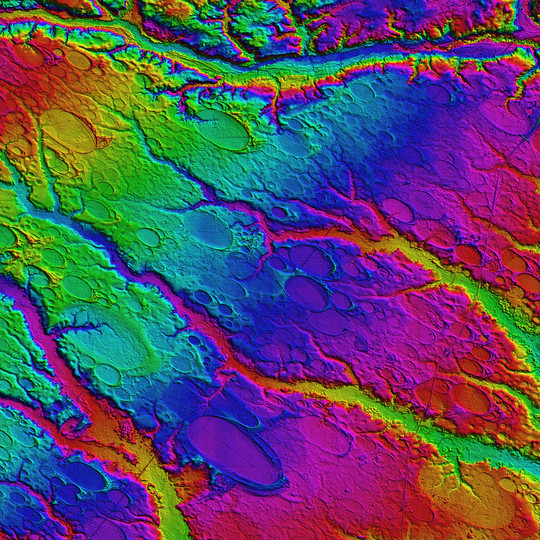
\includegraphics[width=\textwidth]{lidar_carolina}
    \caption{Image \glssymbol{Lidar} de la Caroline du Nord (États-Unis). Le codage couleur correspond à l'élévation topographique.\\
    \small \href{https://commons.wikimedia.org/wiki/File:Rex,_NC_LiDAR_DEM_of_Carolina_bays.jpg}{Crédits images : Cintos (domaine public, Wikimédia Commons)}
    }
  \end{subfigure}
  \begin{subfigure}[t]{0.33\textwidth}
    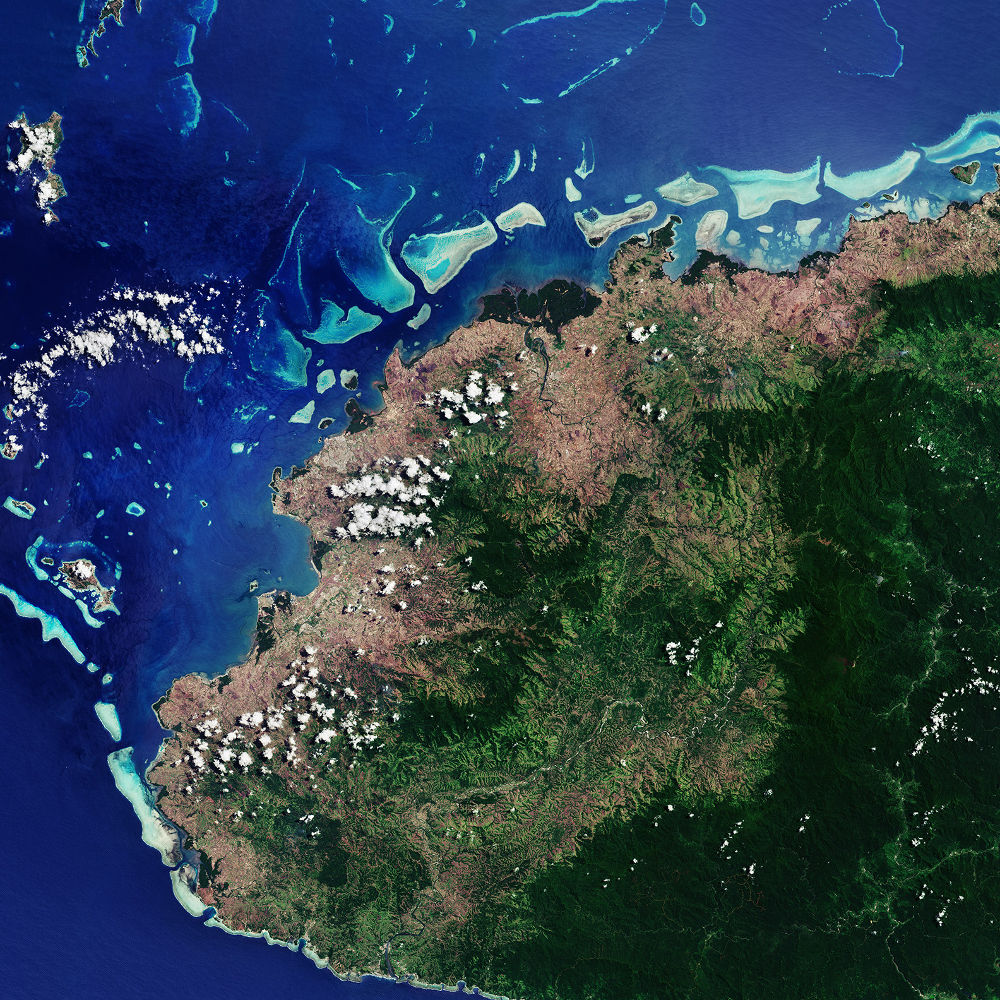
\includegraphics[width=\textwidth]{Sentinel2_Viti_Levu_Fiji}
    \caption{Composition \glssymbol{RVB} d'une image multispectrale Sentinel-2 sur l'île de Viti Levu (Fiji).\\
    \small \href{https://www.esa.int/spaceinimages/Images/2017/11/Viti_Levu_Fiji}{Crédits images : données Copernicus Sentinel, traitées par l'ESA (CC BY-SA 3.0 IGO)}
    }
  \end{subfigure}
  \begin{subfigure}[t]{0.33\textwidth}
    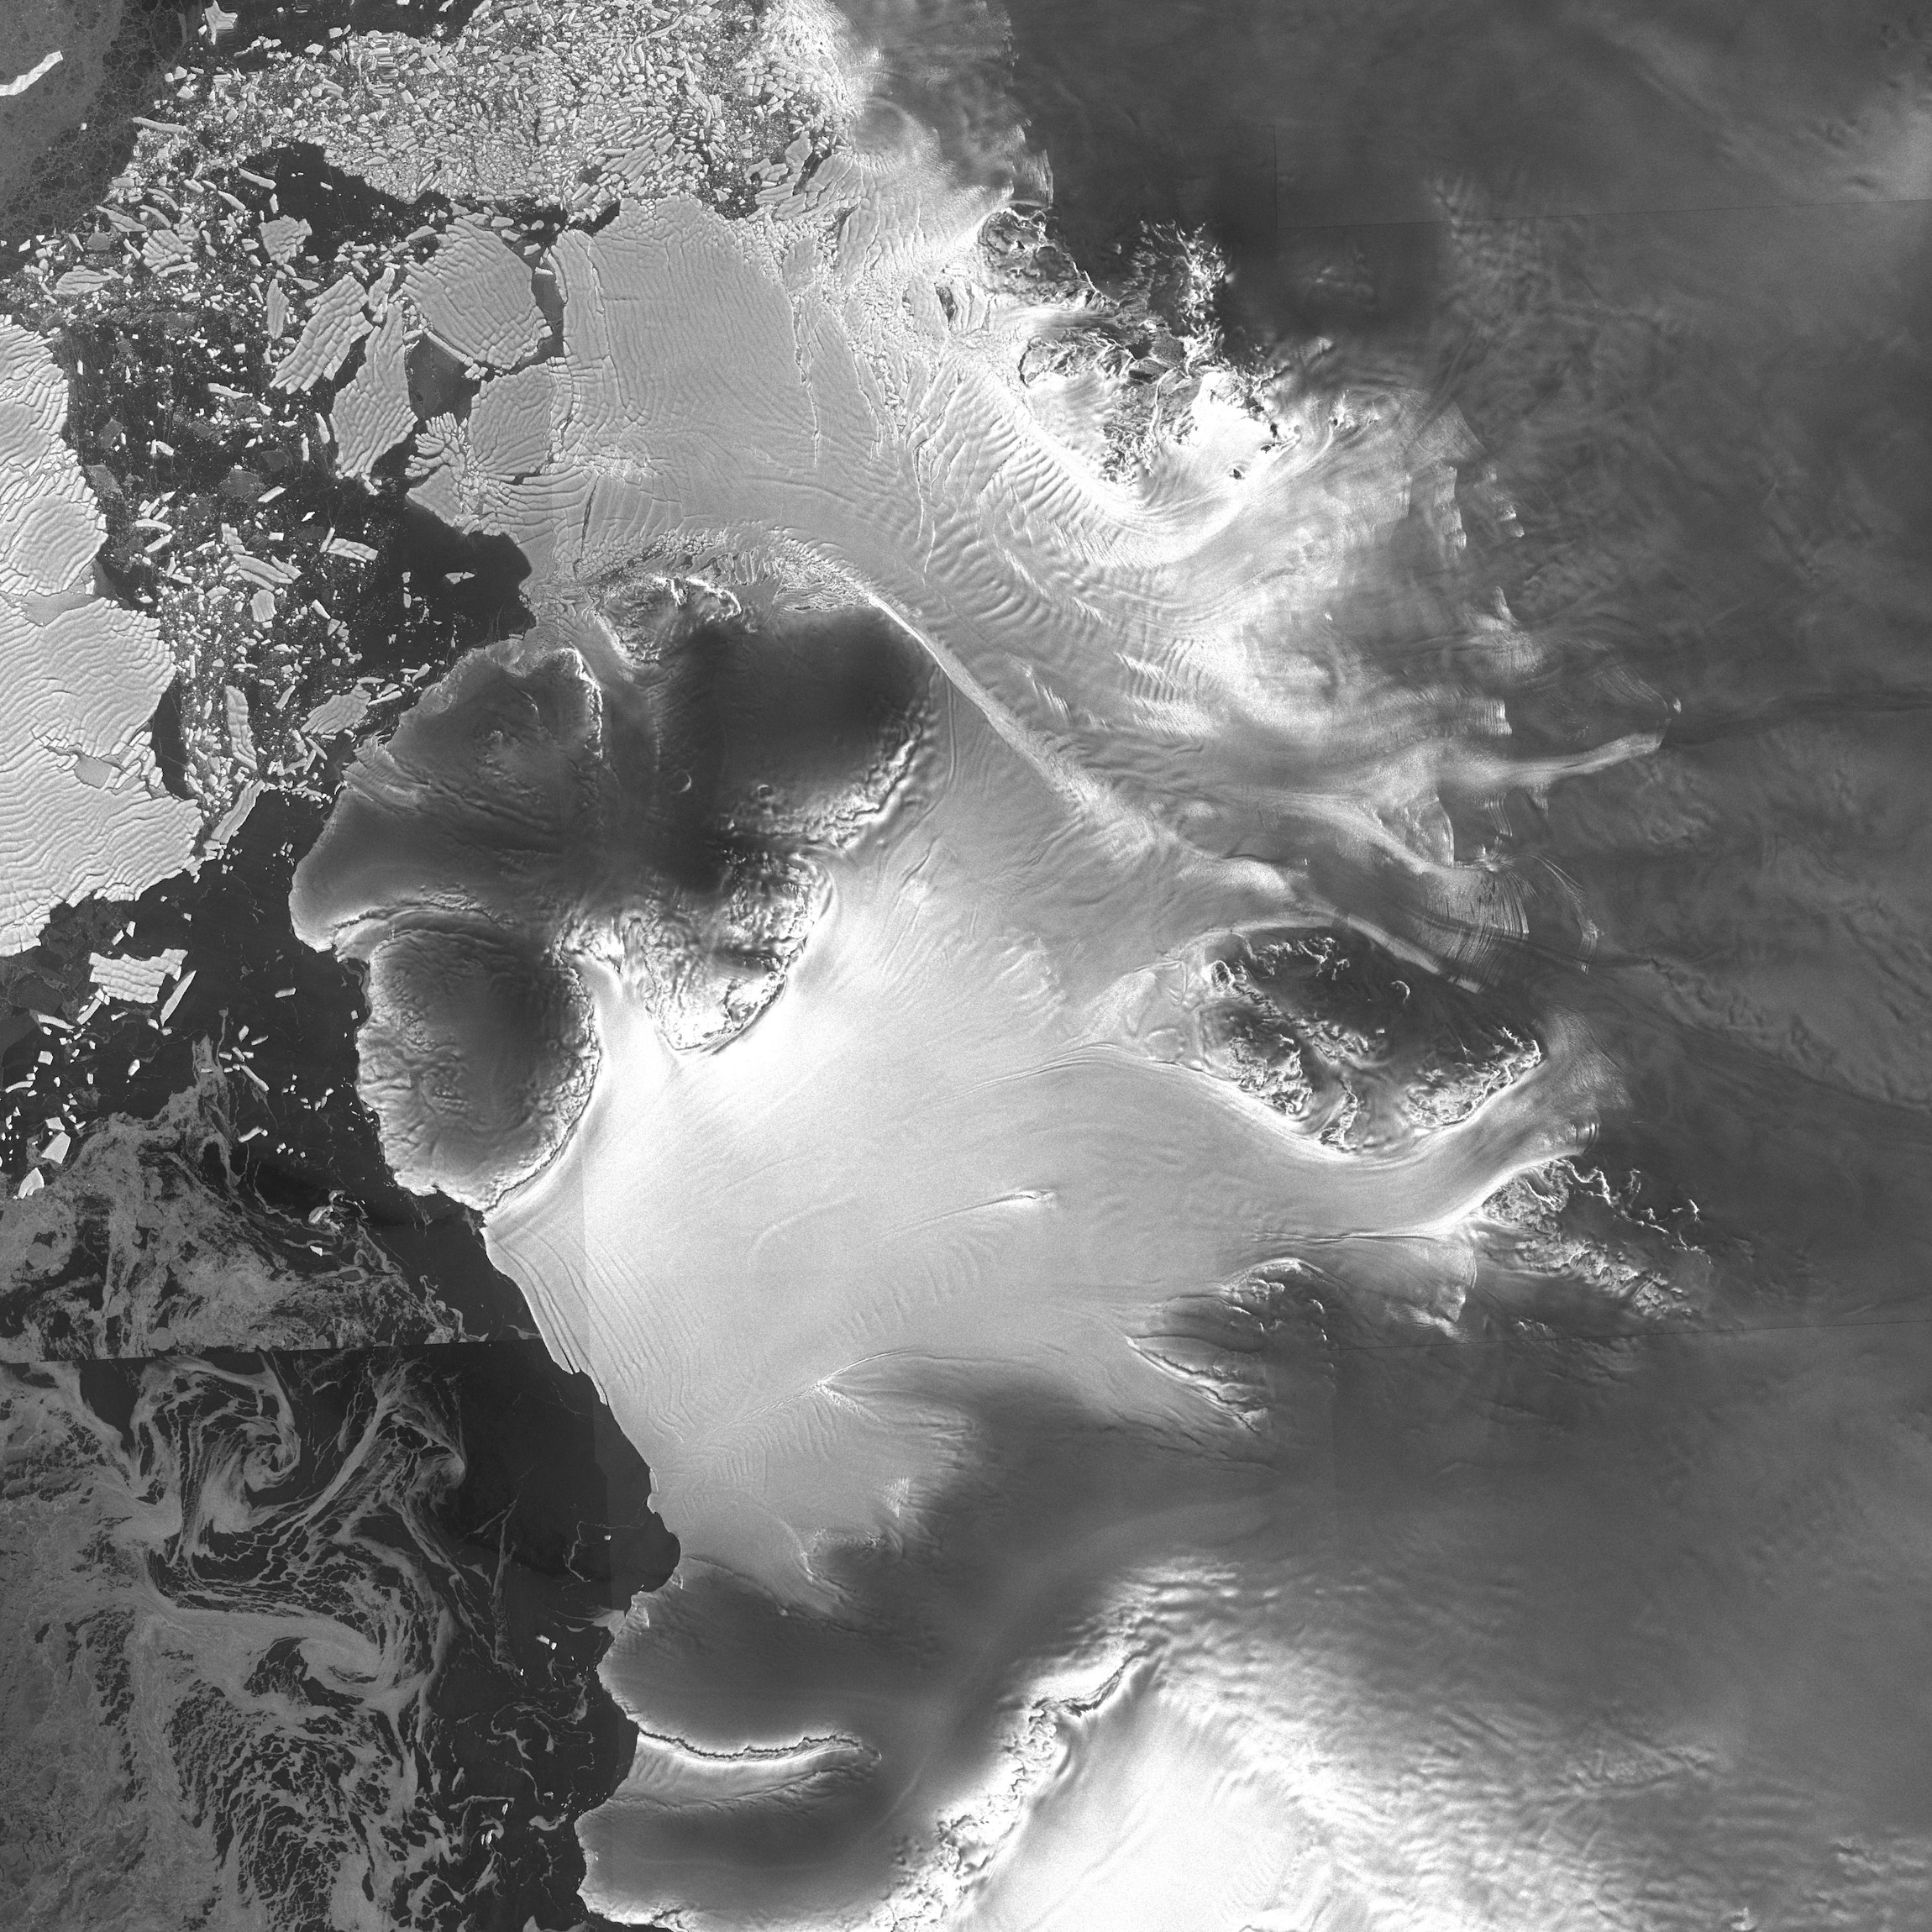
\includegraphics[width=\textwidth]{Sentinel1_Dotson_ice_shelf}
    \caption{Image \glssymbol{SAR} Sentinel-1 de la barrière de glace de Dotson (Antarctique).\\
    \small \href{https://www.esa.int/spaceinimages/Images/2017/10/Dotson_ice_shelf_from_Sentinel-1}{Crédits images : données Copernicus Sentinel, traitées par A. Hogg/CPOM}
    }
  \end{subfigure}
  \caption{L'observation de la Terre implique une grande variété de capteurs dotés de spécificités qui leur sont propres.}
  \label{fig:earth_observation}
\end{figure}

\section{Apprentissage pour le traitement d'images de télédétection}

L'interprétation d'images de télédétection mobilise des fonctions cognitives similaires à celles utilisées pour la compréhension de photographies de la vie quotidienne. Les outils de traitement d'images et de vision artificielle sont ainsi très largement mis en \oe{}uvre pour l'aide à la photo-interprétation. Cependant, l'observation de la Terre fait appel à des capteurs et à des points de vue très spécifiques. Ainsi, la cartographie automatisée d'images aériennes et satellitaires ne se réduit pas à une branche de la vision artificielle. Il s'agit de l'intersection entre celle-ci et la télédétection pour l'observation de la Terre, recouvrant aussi bien des aspects d'apprentissage automatique pour la vision que du traitement des signaux spécifiques aux capteurs aéroportés et satellites, souvent très éloignés des appareils photos du commerce.

\subsection{Différents types d'imagerie}

La~\cref{fig:earth_observation} présente quelques capteurs illustrant la variété des appareils d'imagerie de télédétection pour l'observation de la Terre. Si les acquisitions aéroportées se font généralement en couleurs \gls{RVB} à l'aide d'appareils photos classiques, les acquisitions satellitaires utilisent bien souvent des capteurs sophistiqués dotés de capacités particulières, comme transmettre une information spectrale riche, percer la couverture nuageuse ou mesurer des propriétés physiques de la surface de la Terre.

Par exemple, l'imagerie infrarouge est souvent utilisée en complément des acquisitions couleur. Il est courant, y compris en aéroporté, d'imager à la fois le domaine visible et le proche infrarouge, situé entre \SI{780}{\nano\meter} et \SI{2 500}{\nano\meter}. En effet, la végétation y a une réponse amplifiée par la présence de chlorophylle ce qui rend ce signal très informatif. Dans l'infrarouge moyen et lointain, il est également possible de mesurer indirectement la température par le biais des radiations lumineuses émises selon la loi de Wien. Ces caméras thermiques sont particulièrement utiles dans l'espace, où l'influence de la chaleur naturelle terrestre est peu présente.

\begin{figure}
  \resizebox{\textwidth}{!}{
  \documentclass{standalone}
\usepackage[utf8]{inputenc}
\usepackage[T1]{fontenc}
\usepackage{tikz}
\usepackage{pgfplots}
%%%%%%%%%%%%%%%%%%%%%%%%%%%%%%%%%%%%%%%%
%           Commandes perso            %
%%%%%%%%%%%%%%%%%%%%%%%%%%%%%%%%%%%%%%%%

%% Figures centrées, et en position 'here, top, bottom or page'
\newenvironment{figureth}{%
		\begin{figure}[htbp]
			\centering
	}{
		\end{figure}
		}


%% Tableaux centrés, et en position 'here, top, bottom or page'
\newenvironment{tableth}{%
		\begin{table}[htbp]
			\centering
			%\rowcolors{1}{coleurtableau}{coleurtableau}
	}{
		\end{table}
		}

%% Sous-figures centrées, en position 'top'
\newenvironment{subfigureth}[1]{%
	\begin{subfigure}[t]{#1}
	\centering
}{
	\end{subfigure}
}

\newcommand{\citationChap}[2]{%
	\epigraph{\og \textit{#1} \fg{}}{#2}
}

%% On commence par une page impaire quand on change le style de numérotation de pages
\let\oldpagenumbering\pagenumbering
\renewcommand{\pagenumbering}[1]{%
	\cleardoublepage
	\oldpagenumbering{#1}
}

%% Légende du dataset ISPRS
\newcommand\isprslegende{
Légende\,: \textcolor{Black}{blanc}\,: routes, \textcolor{Blue}{bleu}\,: bâtiments, \textcolor{Cerulean}{cyan}\,: végétation basse, \textcolor{OliveGreen}{vert}\,: arbres, \textcolor{Dandelion}{jaune}\,: véhicules, \textcolor{BrickRed}{rouge}\,: autre.
}

%% Dessiner des réseaux de neurones avec Tikz
\newcommand{\convlayer}[9]{%{h}{w}{d}{name}{color}{x}{y}{z}%{note w}{note h}{note d}
   \def\h{#1}
   \def\w{#2}
   \def\d{#3}
   \def\name{#4}
   \ifthenelse {\equal{#5} {}} {\def\col{white}} {\def\col{#5}}
   \def\x{#6}
   \ifthenelse {\equal{#7} {}} {\def\y{0}} {\def\y{#7}}
   \ifthenelse {\equal{#8} {}} {\def\z{0}} {\def\z{#8}}
   % ne faites pas ça chez vous !
   \ifthenelse {\equal{#9} {}} {\convlayercontinued{}{}{}} {\convlayercontinued#9}
}

\newcommand\convlayercontinued[3]{
   \def\notew{#1}
   \def\noteh{#2}
   \def\noted{#3}
   \coordinate (A) at (\x-\d/2,  \y-\h/2, \z-\w/2);
   \coordinate (B) at (\x-\d/2,  \y-\h/2, \z+\w/2);
   \coordinate (C) at (\x-\d/2,  \y+\h/2, \z+\w/2);
   \coordinate (D) at (\x-\d/2,  \y+\h/2, \z-\w/2);
   \coordinate (E) at (\x+\d/2,  \y-\h/2, \z-\w/2);
   \coordinate (F) at (\x+\d/2,  \y-\h/2, \z+\w/2);
   \coordinate (G) at (\x+\d/2,  \y+\h/2, \z+\w/2);
   \coordinate (H) at (\x+\d/2,  \y+\h/2, \z-\w/2);

    \draw [draw opacity=0.3, fill opacity=0.8, fill=\col!60!white] (A) -- (B) -- (C) -- (D) -- cycle;
    \draw [draw opacity=0.3, fill opacity=0.8, fill=\col!60!white] (A) -- (B) -- (F) -- (E) -- cycle;
    % Face haut
    %\draw [left color=\col!60!white, right color=\col!80!white, shading=axis, shading angle=180] (C) -- (D)  -- (H) -- (G) -- cycle;
    \draw [fill opacity=0.9, fill=\col!70!white] (C) -- node[rotate=45,above] {\small \name} (D) -- (H) -- (G) -- cycle;
    %\draw [fill opacity=0.9, fill=\col!70!white] (C) -- (D) -- node[above] {\small \name} (H) -- (G) -- cycle;
    % Face droite
    \draw [fill opacity=0.9, fill=\col!60!white] (E) -- node[pos=0.75,rotate=45,below] {\scriptsize \notew} (F) -- (G) --  (H) -- cycle;
    % Face avant
    %\draw [shading=axis, left color=\col!60!white, right color=\col!40!white, shading angle=-45] (B) -- node[above,rotate=90] {\scriptsize \noteh} (C) -- (G) -- (F) -- node[below] {\scriptsize \noted}  cycle;
    \draw [fill opacity=0.9, fill=\col!50!white] (B) -- node[above,rotate=90] {\scriptsize \noteh} (C) -- (G) -- (F) -- node[below] {\scriptsize \noted}  cycle;
}

\newcommand{\fclayer}[8]{%{h}{w}{name}{color}{x}{y}{z}
   \def\h{#1}
   \def\w{#2}
   \def\name{#3}
   \ifthenelse {\equal{#4} {}} {\def\col{white}} {\def\col{#4}}
   \def\x{#5}
   \def\y{#6}
   \def\z{#7}
   \def\note{#8}
   \coordinate (A) at (\x-\w/2,  \y-\h/2, \z);
   \coordinate (B) at (\x+\w/2,  \y-\h/2, \z);
   \coordinate (C) at (\x+\w/2,  \y+\h/2, \z);
   \coordinate (D) at (\x-\w/2,  \y+\h/2, \z);

   \pgfmathparse{4*\w}\let\boxwidth\pgfmathresult
    \draw [fill=\col] (A) -- node[below,text width=\boxwidth cm,align=center] {\scriptsize \note} (B) -- (C) -- (D) -- cycle;

    \node (N) at ($(A)!0.5!(B)+(0,-1,0)$) {\name};
}

\newcommand{\alexnet}[4]{%{scale}{x}{y}{z}
  \def\scale{#1}
  \def\alexx{#2}
  \def\alexy{#3}
  \def\alexz{#4}


  \def\coblue{blue!50!white}
  \def\fcgrey{gray!50!white}

  \convlayer{1.3*\scale}{1.3*\scale}{0.02*\scale}{Image}{\coblue}{\alexx}{\alexy}{\alexz}{{227}{227}{3}}
  \convlayer{1.1*\scale}{1.1*\scale}{0.08*\scale}{Conv1}{\coblue}{\alexx+0.7*\scale}{\alexy}{\alexz}{{55}{55}{96}}
  \convlayer{0.7*\scale}{0.7*\scale}{0.5*\scale}{Conv2}{\coblue}{\alexx+1.5*\scale}{\alexy}{\alexz}{{27}{27}{256}}
  \convlayer{0.5*\scale}{0.5*\scale}{0.8*\scale}{Conv3}{\coblue}{\alexx+2.6*\scale}{\alexy}{\alexz}{{13}{13}{384}}
  \convlayer{0.5*\scale}{0.5*\scale}{0.8*\scale}{Conv4}{\coblue}{\alexx+3.8*\scale}{\alexy}{\alexz}{{13}{13}{384}}
  \convlayer{0.5*\scale}{0.5*\scale}{0.5*\scale}{Conv5}{\coblue}{\alexx+4.8*\scale}{\alexy}{\alexz}{{13}{13}{256}}
  \fclayer{\scale}{0.1*\scale}{FC1}{\fcgrey}{\alexx+5.4*\scale}{\alexy}{\alexz}{4096}
  \fclayer{\scale}{0.1*\scale}{FC2}{\fcgrey}{\alexx+5.7*\scale}{\alexy}{\alexz}{4096}
  \fclayer{\scale}{0.1*\scale}{FC3}{\fcgrey}{\alexx+6.0*\scale}{\alexy}{\alexz}{1000}
}

\newcommand{\imagelayer}[7]{%{width}{x}{y}{z}{path}{text_up}{text_down}
    \pgfmathparse{#1}\let\w\pgfmathresult
    \begin{scope}[canvas is yz plane at x=#2]
     \node[transform shape] (source) at (#3, #4) {\includegraphics[angle=-90,width=\w cm]{#5}};
    \end{scope}
     \node [transform shape, rotate=45, above] at (source.east) {#6};
     \node [transform shape, rotate=45, below] at (source.west) {\scriptsize{#7}};
}

\def\fourier{\mathcal{F}}

\newcommand{\lightspectrum}{%
\pgfplotsset{
    % this *defines* a custom colormap ...
    colormap={slategraywhite}{color(0cm)=(red); color(1cm)=(red); color(2cm)=(red); color(3cm)=(red); color(4cm)=(orange); color(5cm)=(yellow); color(6cm)=(green); color(7cm)=(blue); color(8cm)=(blue); color(9cm)=(purple); color(10cm)=(purple); color(12cm)=(black)}
}
\node at (1.5, 2.7) {\small 1mm};
\node at (4, 3) {Infrarouge};
\node at (7.75, 2.7) {\small 800nm};
\node at (9, 3) {Visible};
\node at (10.5, 2.7) {\small 400nm};
\node at (12, 3) {Ultraviolet};
\node at (13.5, 2.7) {\small 10nm};
\draw[->] (1, 2.5) -- (14, 2.5);
\begin{axis}[hide axis,width=16cm,height=4cm,colormap name=slategraywhite]
\addplot[domain=20:1000,samples=1500,ultra thick, point meta=x*x,mesh]{sin(x*x/80)};
\end{axis}
}

% Union généralisée
\newcommand{\wbigcup}{\mathop{\bigcup}\displaylimits}

\newcommand{\res}[2]{#1 {\footnotesize $\pm$ #2}}
\newcommand{\bres}[2]{\textbf{#1} {\footnotesize $\pm$ #2}}
\newcommand{\bbres}[2]{\res{\textit{#1}}{#2}}

\newcommand{\drawkernel}[9]{
\begin{tikzpicture}
	\draw[step=1cm,gray!50!white,very thin] (0,0) grid (3,3);
	\kernelnode{0.5}{0.5}{#1};
	\kernelnode{0.5}{1.5}{#2};
	\kernelnode{0.5}{2.5}{#3};
	\kernelnode{1.5}{0.5}{#4};
	\kernelnode{1.5}{1.5}{#5};
	\kernelnode{1.5}{2.5}{#6};
	\kernelnode{2.5}{0.5}{#7};
	\kernelnode{2.5}{1.5}{#8};
	\kernelnode{2.5}{2.5}{#9};
\end{tikzpicture}
}

\newcommand{\kernelnode}[3]{%{x}{y}{value}
	\ifthenelse{\equal{#3}{0}}{
		\def\kcolor{gray}
	}{
		\def\kcolor{black}
	}
	\node[\kcolor] at (#1, #2) {#3};
}

\newcommand{\chapsummary}[1]{
\section*{Résumé du chapitre :}
\parbox{0.9\linewidth}{
\setlength{\parindent}{4ex}
#1}
}

\newcommand{\eqname}[1]{\tag*{\small (#1)}}

\begin{document}

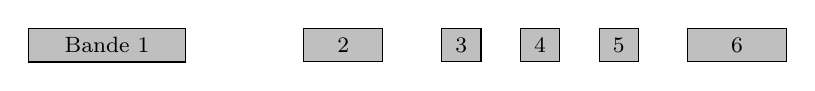
\begin{tikzpicture}
\lightspectrum

\node[draw,fill=gray!50!white,minimum width=2cm,rectangle] at (3.5, -0.2) {\footnotesize Bande 1};
\node[draw,fill=gray!50!white,minimum width=1cm,rectangle] at (6.5, -0.2) {\footnotesize 2};
\node[draw,fill=gray!50!white,minimum width=0.5cm,rectangle] at (8, -0.2) {\footnotesize 3};
\node[draw,fill=gray!50!white,minimum width=0.5cm,rectangle] at (9, -0.2) {\footnotesize 4};
\node[draw,fill=gray!50!white,minimum width=0.5cm,rectangle] at (10, -0.2) {\footnotesize 5};
\node[draw,fill=gray!50!white,minimum width=1.25cm,rectangle] at (11.5, -0.2) {\footnotesize 6};
\end{tikzpicture}
\end{document}

  }
  \caption{Un capteur multispectral acquiert plusieurs bandes spectrales larges réparties sur le spectre lumineux infrarouge, visible et parfois ultraviolet.}
  \label{fig:multispectral}
\end{figure}

La~\cref{fig:multispectral} illustre une \glsfirst{multispectral} ou superspectrale qui, selon ce même principe, permet d'imager une scène dans plusieurs bandes de longueurs d'ondes plus ou moins larges pouvant se trouver aussi bien dans le domaine visible que dans l'infrarouge ou l'ultraviolet. Cela conduit à des images à plusieurs canaux, généralement une dizaine, qui ne sont donc pas directement visualisables par l'\oe{}il humain. Il est toutefois possible de reconstituer une image en couleurs naturelles en recomposant une image \gls{RVB} à partir des valeurs contenues dans les canaux correspondant aux longueurs d'onde du rouge, du vert et du bleu. Les acquisitions multispectrales peuvent avoir des résolutions différentes en fonction des canaux. Les satellites Sentinel-2A et Sentinel-2B produisent par exemple des images à une résolution au sol de \SI{10}{\meter/\px} dans le domaine visible, mais certaines bandes, notamment dans l'infrarouge, ont des résolutions de \SI{20}{\meter/\px} ou \SI{60}{\meter/\px}. Les acquisitions couleurs satellitaires les mieux résolues spatialement ont une résolution au sol de l'ordre de \SI{30}{\centi\meter/\px}, tandis que les images aéroportées peuvent aller jusqu'à une résolution de \SI{5}{\centi\meter/\px}. Dans le cas des acquisitions satellitaires, il est courant de réaliser en simultané une mesure multispectrale et une acquisition panchromatique, c'est-à-dire qui ne distingue pas les couleurs et produit une image en noir et blanc, à résolution supérieure. Ainsi, \gls{Pleiades} réalise à la fois une acquisition panchromatique à résolution \SI{70}{\centi\meter/\px}, ré-échantillonnée à \SI{50}{\centi\meter/\px} et multispectrale à \SI{2,8}{\meter/\px} rééchantillonnée à \SI{2}{\meter/\px}.

\begin{figure}
  \resizebox{\textwidth}{!}{
  \documentclass{standalone}
\usepackage[utf8]{inputenc}
\usepackage[T1]{fontenc}
\usepackage{tikz}
\usepackage{pgfplots}
%%%%%%%%%%%%%%%%%%%%%%%%%%%%%%%%%%%%%%%%
%           Commandes perso            %
%%%%%%%%%%%%%%%%%%%%%%%%%%%%%%%%%%%%%%%%

%% Figures centrées, et en position 'here, top, bottom or page'
\newenvironment{figureth}{%
		\begin{figure}[htbp]
			\centering
	}{
		\end{figure}
		}


%% Tableaux centrés, et en position 'here, top, bottom or page'
\newenvironment{tableth}{%
		\begin{table}[htbp]
			\centering
			%\rowcolors{1}{coleurtableau}{coleurtableau}
	}{
		\end{table}
		}

%% Sous-figures centrées, en position 'top'
\newenvironment{subfigureth}[1]{%
	\begin{subfigure}[t]{#1}
	\centering
}{
	\end{subfigure}
}

\newcommand{\citationChap}[2]{%
	\epigraph{\og \textit{#1} \fg{}}{#2}
}

%% On commence par une page impaire quand on change le style de numérotation de pages
\let\oldpagenumbering\pagenumbering
\renewcommand{\pagenumbering}[1]{%
	\cleardoublepage
	\oldpagenumbering{#1}
}

%% Légende du dataset ISPRS
\newcommand\isprslegende{
Légende\,: \textcolor{Black}{blanc}\,: routes, \textcolor{Blue}{bleu}\,: bâtiments, \textcolor{Cerulean}{cyan}\,: végétation basse, \textcolor{OliveGreen}{vert}\,: arbres, \textcolor{Dandelion}{jaune}\,: véhicules, \textcolor{BrickRed}{rouge}\,: autre.
}

%% Dessiner des réseaux de neurones avec Tikz
\newcommand{\convlayer}[9]{%{h}{w}{d}{name}{color}{x}{y}{z}%{note w}{note h}{note d}
   \def\h{#1}
   \def\w{#2}
   \def\d{#3}
   \def\name{#4}
   \ifthenelse {\equal{#5} {}} {\def\col{white}} {\def\col{#5}}
   \def\x{#6}
   \ifthenelse {\equal{#7} {}} {\def\y{0}} {\def\y{#7}}
   \ifthenelse {\equal{#8} {}} {\def\z{0}} {\def\z{#8}}
   % ne faites pas ça chez vous !
   \ifthenelse {\equal{#9} {}} {\convlayercontinued{}{}{}} {\convlayercontinued#9}
}

\newcommand\convlayercontinued[3]{
   \def\notew{#1}
   \def\noteh{#2}
   \def\noted{#3}
   \coordinate (A) at (\x-\d/2,  \y-\h/2, \z-\w/2);
   \coordinate (B) at (\x-\d/2,  \y-\h/2, \z+\w/2);
   \coordinate (C) at (\x-\d/2,  \y+\h/2, \z+\w/2);
   \coordinate (D) at (\x-\d/2,  \y+\h/2, \z-\w/2);
   \coordinate (E) at (\x+\d/2,  \y-\h/2, \z-\w/2);
   \coordinate (F) at (\x+\d/2,  \y-\h/2, \z+\w/2);
   \coordinate (G) at (\x+\d/2,  \y+\h/2, \z+\w/2);
   \coordinate (H) at (\x+\d/2,  \y+\h/2, \z-\w/2);

    \draw [draw opacity=0.3, fill opacity=0.8, fill=\col!60!white] (A) -- (B) -- (C) -- (D) -- cycle;
    \draw [draw opacity=0.3, fill opacity=0.8, fill=\col!60!white] (A) -- (B) -- (F) -- (E) -- cycle;
    % Face haut
    %\draw [left color=\col!60!white, right color=\col!80!white, shading=axis, shading angle=180] (C) -- (D)  -- (H) -- (G) -- cycle;
    \draw [fill opacity=0.9, fill=\col!70!white] (C) -- node[rotate=45,above] {\small \name} (D) -- (H) -- (G) -- cycle;
    %\draw [fill opacity=0.9, fill=\col!70!white] (C) -- (D) -- node[above] {\small \name} (H) -- (G) -- cycle;
    % Face droite
    \draw [fill opacity=0.9, fill=\col!60!white] (E) -- node[pos=0.75,rotate=45,below] {\scriptsize \notew} (F) -- (G) --  (H) -- cycle;
    % Face avant
    %\draw [shading=axis, left color=\col!60!white, right color=\col!40!white, shading angle=-45] (B) -- node[above,rotate=90] {\scriptsize \noteh} (C) -- (G) -- (F) -- node[below] {\scriptsize \noted}  cycle;
    \draw [fill opacity=0.9, fill=\col!50!white] (B) -- node[above,rotate=90] {\scriptsize \noteh} (C) -- (G) -- (F) -- node[below] {\scriptsize \noted}  cycle;
}

\newcommand{\fclayer}[8]{%{h}{w}{name}{color}{x}{y}{z}
   \def\h{#1}
   \def\w{#2}
   \def\name{#3}
   \ifthenelse {\equal{#4} {}} {\def\col{white}} {\def\col{#4}}
   \def\x{#5}
   \def\y{#6}
   \def\z{#7}
   \def\note{#8}
   \coordinate (A) at (\x-\w/2,  \y-\h/2, \z);
   \coordinate (B) at (\x+\w/2,  \y-\h/2, \z);
   \coordinate (C) at (\x+\w/2,  \y+\h/2, \z);
   \coordinate (D) at (\x-\w/2,  \y+\h/2, \z);

   \pgfmathparse{4*\w}\let\boxwidth\pgfmathresult
    \draw [fill=\col] (A) -- node[below,text width=\boxwidth cm,align=center] {\scriptsize \note} (B) -- (C) -- (D) -- cycle;

    \node (N) at ($(A)!0.5!(B)+(0,-1,0)$) {\name};
}

\newcommand{\alexnet}[4]{%{scale}{x}{y}{z}
  \def\scale{#1}
  \def\alexx{#2}
  \def\alexy{#3}
  \def\alexz{#4}


  \def\coblue{blue!50!white}
  \def\fcgrey{gray!50!white}

  \convlayer{1.3*\scale}{1.3*\scale}{0.02*\scale}{Image}{\coblue}{\alexx}{\alexy}{\alexz}{{227}{227}{3}}
  \convlayer{1.1*\scale}{1.1*\scale}{0.08*\scale}{Conv1}{\coblue}{\alexx+0.7*\scale}{\alexy}{\alexz}{{55}{55}{96}}
  \convlayer{0.7*\scale}{0.7*\scale}{0.5*\scale}{Conv2}{\coblue}{\alexx+1.5*\scale}{\alexy}{\alexz}{{27}{27}{256}}
  \convlayer{0.5*\scale}{0.5*\scale}{0.8*\scale}{Conv3}{\coblue}{\alexx+2.6*\scale}{\alexy}{\alexz}{{13}{13}{384}}
  \convlayer{0.5*\scale}{0.5*\scale}{0.8*\scale}{Conv4}{\coblue}{\alexx+3.8*\scale}{\alexy}{\alexz}{{13}{13}{384}}
  \convlayer{0.5*\scale}{0.5*\scale}{0.5*\scale}{Conv5}{\coblue}{\alexx+4.8*\scale}{\alexy}{\alexz}{{13}{13}{256}}
  \fclayer{\scale}{0.1*\scale}{FC1}{\fcgrey}{\alexx+5.4*\scale}{\alexy}{\alexz}{4096}
  \fclayer{\scale}{0.1*\scale}{FC2}{\fcgrey}{\alexx+5.7*\scale}{\alexy}{\alexz}{4096}
  \fclayer{\scale}{0.1*\scale}{FC3}{\fcgrey}{\alexx+6.0*\scale}{\alexy}{\alexz}{1000}
}

\newcommand{\imagelayer}[7]{%{width}{x}{y}{z}{path}{text_up}{text_down}
    \pgfmathparse{#1}\let\w\pgfmathresult
    \begin{scope}[canvas is yz plane at x=#2]
     \node[transform shape] (source) at (#3, #4) {\includegraphics[angle=-90,width=\w cm]{#5}};
    \end{scope}
     \node [transform shape, rotate=45, above] at (source.east) {#6};
     \node [transform shape, rotate=45, below] at (source.west) {\scriptsize{#7}};
}

\def\fourier{\mathcal{F}}

\newcommand{\lightspectrum}{%
\pgfplotsset{
    % this *defines* a custom colormap ...
    colormap={slategraywhite}{color(0cm)=(red); color(1cm)=(red); color(2cm)=(red); color(3cm)=(red); color(4cm)=(orange); color(5cm)=(yellow); color(6cm)=(green); color(7cm)=(blue); color(8cm)=(blue); color(9cm)=(purple); color(10cm)=(purple); color(12cm)=(black)}
}
\node at (1.5, 2.7) {\small 1mm};
\node at (4, 3) {Infrarouge};
\node at (7.75, 2.7) {\small 800nm};
\node at (9, 3) {Visible};
\node at (10.5, 2.7) {\small 400nm};
\node at (12, 3) {Ultraviolet};
\node at (13.5, 2.7) {\small 10nm};
\draw[->] (1, 2.5) -- (14, 2.5);
\begin{axis}[hide axis,width=16cm,height=4cm,colormap name=slategraywhite]
\addplot[domain=20:1000,samples=1500,ultra thick, point meta=x*x,mesh]{sin(x*x/80)};
\end{axis}
}

% Union généralisée
\newcommand{\wbigcup}{\mathop{\bigcup}\displaylimits}

\newcommand{\res}[2]{#1 {\footnotesize $\pm$ #2}}
\newcommand{\bres}[2]{\textbf{#1} {\footnotesize $\pm$ #2}}
\newcommand{\bbres}[2]{\res{\textit{#1}}{#2}}

\newcommand{\drawkernel}[9]{
\begin{tikzpicture}
	\draw[step=1cm,gray!50!white,very thin] (0,0) grid (3,3);
	\kernelnode{0.5}{0.5}{#1};
	\kernelnode{0.5}{1.5}{#2};
	\kernelnode{0.5}{2.5}{#3};
	\kernelnode{1.5}{0.5}{#4};
	\kernelnode{1.5}{1.5}{#5};
	\kernelnode{1.5}{2.5}{#6};
	\kernelnode{2.5}{0.5}{#7};
	\kernelnode{2.5}{1.5}{#8};
	\kernelnode{2.5}{2.5}{#9};
\end{tikzpicture}
}

\newcommand{\kernelnode}[3]{%{x}{y}{value}
	\ifthenelse{\equal{#3}{0}}{
		\def\kcolor{gray}
	}{
		\def\kcolor{black}
	}
	\node[\kcolor] at (#1, #2) {#3};
}

\newcommand{\chapsummary}[1]{
\section*{Résumé du chapitre :}
\parbox{0.9\linewidth}{
\setlength{\parindent}{4ex}
#1}
}

\newcommand{\eqname}[1]{\tag*{\small (#1)}}

\begin{document}

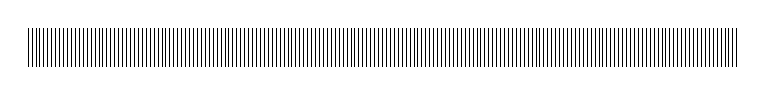
\begin{tikzpicture}
\lightspectrum

\foreach \x in {300,305,...,1200}{
\fill (\x/100, -0.5) rectangle (\x/100+0.01, 0.);
}
\end{tikzpicture}
\end{document}

  }
  \caption{Un capteur hyperspectral acquiert de nombreuses bandes spectrales étroites régulièrement réparties sur sa plage d'acquisition.}
  \label{fig:hyperspectral}
\end{figure}

L'\glsfirst{hyperspectral} consiste à effectuer des acquisitions sur de nombreuses bandes étroites, toutes de même taille, afin de balayer de façon discrète l'ensemble du spectre lumineux réfléchi, comme illustré par la~\cref{fig:hyperspectral}. En fonction de la résolution spectrale -- souvent de l'ordre de \SI{10}{\nano\meter} -- et de la largeur du spectre considéré, le nombre de bandes peut varier de quelques dizaines à plusieurs centaines. L'intérêt de ces caméras réside dans la possibilité de reconstituer la courbe de l'intensité lumineuse réfléchie en fonction de la longueur d'onde pour chaque pixel. En effet, tous les matériaux réfléchissent différemment la lumière du Soleil en fonction de leur albédo. Cette information permet donc de caractériser finement la composition physique des objets observés. En contrepartie, la résolution spatiale des caméras hyperspectrales est nettement plus faible que celle des autres appareils optiques. Les acquisitions hyperspectrales présentent de fait une résolution au sol d'environ \SI{1}{\meter/\px} en aérien et \SI{30}{\meter/\px} en satellite.

Notons que l'ensemble des capteurs optiques présentés ci-dessus sont passifs; ils ne reçoivent que l'énergie lumineuse réfléchie ou émise par le corps observé. Par conséquent, ces capteurs sont sensibles aux variations d'illumination et aux effets météorologiques, les nuages pouvant notamment les rendre entièrement inopérationnels. De nombreux autres satellites sont munis de capteurs actifs qui émettent un signal dont ils mesurent le retour. C'est notamment le cas des satellites radar, et en particulier \gls{SAR}, qui envoient une ou plusieurs ondes électromagnétiques et utilisent la mesure de l'onde réfléchie pour extraire des paramètres physiques de la zone observée. Le \gls{SAR} permet ainsi de percer la couverture nuageuse, mais ne produit des images à proprement parler.

\begin{figure}
  % \resizebox{\textwidth}{!}{
  % \input{Chapitre1/mnt.pdf_tex}
  % }
  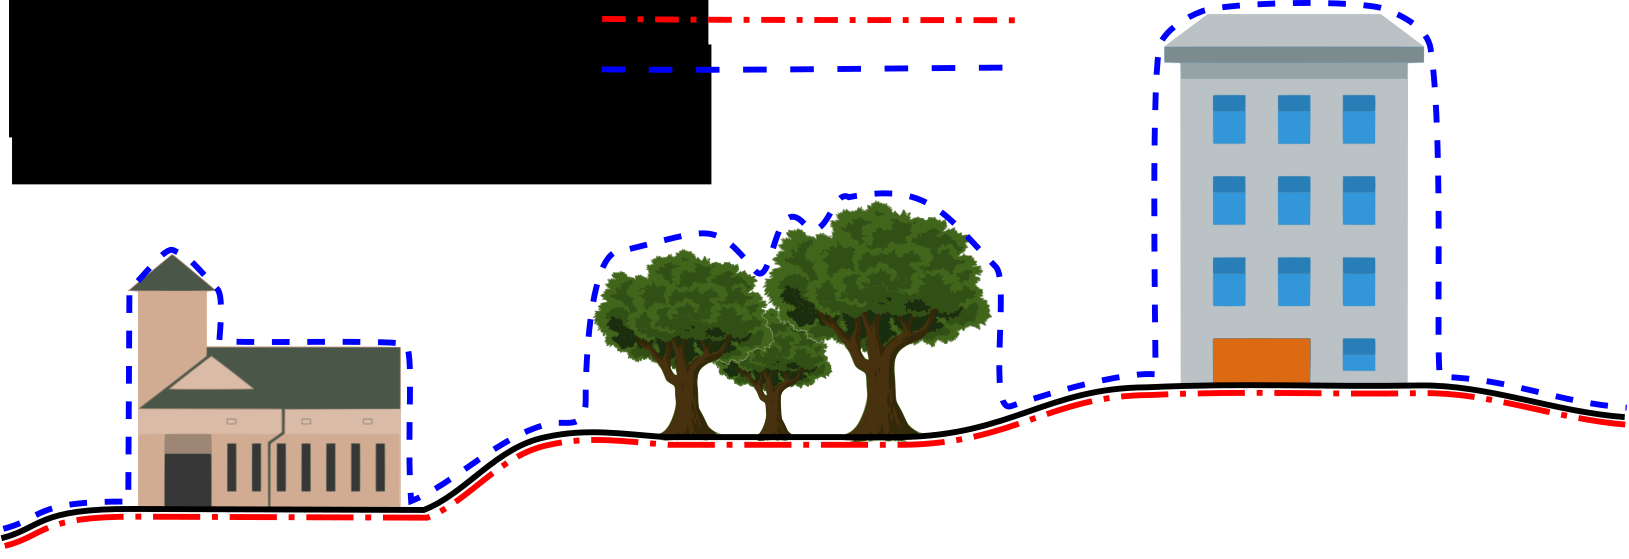
\includegraphics[width=\textwidth]{mnt.pdf}
  \caption{Schéma représentatif de la différence entre \glsname{MNT} et \glsname{MNE}.}
  \label{fig:mnt}
\end{figure}

Le \gls{Lidar} est un autre capteur actif, qui émet une impulsion laser dont il mesure l'écho. La position du maximum d'amplitude permet de déterminer le temps d'aller-retour du rayon lumineux et donc de mesurer la distance parcourue par les photons. Ces capteurs sont très utilisés en télédétection comme en robotique afin d'effectuer des relevés topographiques ou des reconstructions 3D. La nature ponctuelle de la mesure laser ne permet cependant de construire que des nuages de points faiblement denses. Dans le cas du \gls{Lidar} satellitaire, les mesures se font tous les \SI{20}{\meter}, et tous les \SI{10}{\centi\meter} dans le cas de l'aéroporté. Une fois le nuage de points construit, il est possible d'en extraire un maillage qui modélise la topographie de la surface observée. Celui-ci peut alors être rastérisé, c'est-à-dire projeté sur un plan, pour obtenir un \glsfirst{MNT} ou un \glsfirst{MNE} en fonction de la résolution. Le \gls{MNE} se distingue du \gls{MNT} en ce qu'il prend en compte les objets surélevés par-dessus la surface topographique, un exemple étant exposé dans la~\cref{fig:mnt}. La différence entre ces deux valeurs est appelée \glsfirst{MNH} et correspond à la hauteur normalisée des points au-dessus du sol.

Les travaux présentés dans ce manuscrit portent principalement sur l'utilisation de données optiques pour la cartographie automatisée. Nous nous autoriserons néanmoins à faire appel à des données ancillaires, qu'elles soient dérivées d'acquisitions \gls{Lidar} ou provenant de \glspl{SIG}.

\subsection{Apprentissage et images de télédétection}

Comme nous venons de le voir, les images de télédétection peuvent se présenter sous des formes variées\,: \glspl{multispectral}, \glspl{hyperspectral}, \gls{SAR}, \gls{Lidar}\dots De nombreuses techniques d'apprentissage automatique ont été mises en \oe{}uvre pour extraire de l'information de ces données sans intervention humaine.

\subsubsection{Extraction de caractéristiques}

Une fois les données acquises et mises en forme, il est nécessaire de choisir une méthode de représentation adaptée à la classification. Plus précisément, il s'agit de décider d'un espace de représentation dans lequel projeter les données, de manière à ce qu'il soit aisé de partitionner l'espace afin d'y séparer les différentes classes. Nous présentons ci-dessous plusieurs approches couramment mises en \oe{}uvre.

Une première méthode consiste à directement utiliser les données brutes, éventuellement normalisées. Le classifieur opère directement sur les valeurs de luminance ou de réflectance des pixels. Cependant, une image \gls{RVB} de dimensions $128\times128$ est alors décrite par $128\times128\times3 = 49152$ scalaires, ce qui est intractable pour la plupart des modèles statistiques usuels. Cela impose alors de traiter les pixels individuellement ou de découper l'image en régions de petite taille. De telles approches sont fréquentes pour le traitement de données hyperspectrales~\cite{fauvel_advances_2013,ham_investigation_2005} et multispectrales, y compris \gls{IRRVB}~\cite{dechesne_semantic_2017}.

En effet, il est possible de combiner les données brutes à des caractéristiques expertes, comme les moments statistiques ou le gradient du signal. Dans le cas des images \gls{Lidar}, l'écart local à la hauteur moyenne est un indicateur souvent adopté pour discriminer différents types d'objets~\cite{guo_relevance_2011,li_lidar_2017,guennec_classication_2018}, et l'entropie locale est une caractéristique classique de l'imagerie \gls{SAR}~\cite{g._barber_sar_1991}.

En outre, les capteurs multispectraux et \gls{SAR} présentent des propriétés physiques dont la connaissance \emph{a priori} est exploitable. Des rapports de réflectance dans différentes longueurs d'onde peuvent permettre de caractériser certaines surfaces, comme le \gls{NDVI}~\cite{rouse_monitoring_1974} pour la végétation et le \gls{NDWI}~\cite{xie_new_2014} pour l'eau. Ces indices sont facilement interprétables mais savoir lesquels utiliser demande une connaissance experte des phénomènes étudiés (il est impossible de détecter un phénomène que l'on ne saurait pas caractériser physiquement, au moins partiellement) et un effort systématique d'ingénierie, puisque ces indices dépendent du problème considéré.

Comme pour le traitement d'images multimédia, il est peut être intéressant de rechercher des caractéristiques génériques. Les histogrammes de couleurs peuvent par exemple s'appliquer à des images multispectrales ou hyperspectrales de la même façon qu'ils s'appliquent aux images \gls{RVB}. De tels histogrammes sont invariants aux rotations et aux translations locales, ainsi qu'aux changements d'échelle. Toutefois, ils sont fortement influencés par les changements radiométriques induits par l'environnement, comme la variation de la luminosité extérieure. Qui plus est, si la discrétisation des valeurs dans l'histogramme ajoute une robustesse au bruit, elle diminue la précision des valeurs numériques et risque de faire disparaître des différences subtiles entre spectres. Dans le cas de l'hyperspectral, deux plastiques peuvent présenter des profils spectraux très similaires, ne différant que par la position de leurs pics d'absorption. Une quantification trop importante peut alors faire disparaître ces pics et donc l'information discriminante. D'autres histogrammes usuels, comme les \gls{HOG}~\cite{dalal_histograms_2005} s'appliquent également aux images de télédétection.

Enfin, les profils morphologiques ont également été fréquemment étudiés pour la classification d'images de télédétection. En particulier, les travaux de~\citet{benediktsson_classification_2003} ont introduit ces descripteurs, obtenus par l'application successive d'opérations morphologiques d'érosion et de dilatation. Ces caractéristiques ont l'avantage de renseigner sur l'appartenance d'un pixel à des structures spatiales à différentes échelles.

En pratique, il est courant d'utiliser une combinaison de ces différentes caractéristiques, en les calculant par exemple sur une pyramide d'images multi-échelle. Une fois les vecteurs de caractéristiques générés, de nombreux modèles statistiques peuvent alors être appliqués.

\subsubsection{Modèles statistiques usuels}

Une fois le vecteur de caractéristiques extrait pour un échantillon, celui-ci sert alors d'entrée à un classifieur. Le classifieur est un modèle statistique de décision pouvant prendre plusieurs formes. Cette partie ne traite que des classifieurs sans apprentissage de représentation, excluant par conséquent les réseaux de neurones profonds qui seront discutés plus tard.

La littérature en apprentissage automatique pour la télédétection a longtemps plébiscité les arbres de décision sous forme de forêts aléatoires~\cite{breiman_random_2001} et les \gls{SVM}~\cite{boser_training_1992,cortes_support-vector_1995}.

Les arbres de décision~\cite{breiman_classification_2017} forment un ensemble de modèles statistiques représentant les variables sous forme de n\oe{}ud intérieur, chaque arête correspondant à un ensemble de valeurs possibles pour la variable associée au n\oe{}ud. L'ensemble des arêtes partant d'un n\oe{}ud donné couvre l'ensemble des valeurs que peut prendre la variable qui lui est associée. Durant la phase d'apprentissage, l'arbre est construit par partitionnement récursif, divisant l'ensemble des données en fonction d'une première variable, puis de la seconde et ainsi de suite jusqu'à ce que l'ajout de variable n'améliore plus la prédiction, ou que tous les sous-ensembles aboutissent au même résultat.

Les arbres de décision sont couramment utilisés sous forme de forêts aléatoires~\cite{breiman_random_2001}. Une forêt aléatoire est en réalité un ensemble d'arbres de décisions construits à partir de sous-ensembles aléatoires des variables d'entrée. Chaque arbre réalise sa prédiction indépendamment des autres, et la prédiction finale est celle ayant obtenu le plus de votes. Réaliser un tel apprentissage par ensemble permet d'obtenir un classifieur dont la variance est plus faible que chaque arbre individuel. Les arbres de décision ont l'avantage d'être simples à interpréter, puisqu'une décision (un n\oe{}ud) est associée à un test sur une caractéristique précise. Les forêts aléatoires ont ainsi été abondamment utilisées en télédétection pour la cartographie d'occupation des sols à partir d'images \gls{Landsat}~\cite{pal_random_2005} et la prédiction météorologique~\cite{lary_machine_2016}. Les ensembles d'arbres de décision ont également été mis en \oe{}uvre sur le principe du \emph{gradient boosting}, permettant d'exploiter un ensemble de modèles de prédiction faibles pour les combiner et renforcer leur pouvoir prédictif~\cite{friedman_greedy_2001}. Ce type de classifieurs est plus rare en télédétection mais se retrouve néanmoins dans certaines applications~\cite{lawrence_classification_2004}.

Les \gls{SVM}~\cite{boser_training_1992,cortes_support-vector_1995} sont des classifieurs partitionnant l'espace de telle sorte que la distance entre la frontière et l'échantillon le plus proche (la marge) soit maximale. La frontière se représente sous la forme d'un hyperplan dans l'espace des données d'entrée dans le cas du noyau linéaire, ou d'un hyperplan dans un espace de représentation de grande dimension (possiblement infinie) en utilisant l'astuce du noyau~\cite{boser_training_1992}.

Si où la dimension des données d'entrée est de grande taille, le calcul exact des hyperplans à marge maximale n'est pas nécessairement réalisable en temps raisonnable. Dans ce cas, il est possible de faire appel à des algorithmes d'approximation reposant sur une optimisation par descente de gradient~\cite{bottou_large-scale_2010}.

Les \gls{SVM} ont trouvé de nombreuses applications en télédétection, notamment pour l'occupation des sols à partir d'images multispectrales~\cite{pal_support_2005} et hyperspectrales~\cite{melgani_classification_2004}.

Enfin, on retrouve également des réseaux de neurones de type perceptron multi-couche dans la littérature pour le traitement d'images multispectrales~\cite{benediktsson_neural_1990} et hyperspectrales~\cite{goel_classification_2003}.

\subsubsection{Caractéristiques spatiales et caractéristiques spectrales}

Comme nous l'avons vu, les caractéristiques expertes de la littérature en télédétection s'intéressent essentiellement à l'information radiométrique. La plupart des méthodes produisent ainsi une classification pixel à pixel, c'est-à-dire que les classifieurs ne réalisent qu'une seule prédiction à la fois, généralement pour le pixel central d'une région considérée.

Si cette approche garantit que les prédictions auront une résolution identique à celle de la donnée, cela ne permet pas de modéliser les relations spatiales entre objets. Compte-tenu de l'augmentation continue de la résolution des capteurs, les objets d'intérêt s'étendent souvent sur plusieurs pixels et présentent des propriétés géométriques particulières de connexité et de convexité. Ainsi, un pixel particulier soumis à un bruit extrême (suite à une défaillance du capteur ou à un matériau particulier) peut être mal classifié s'il est considéré isolément. Un modèle considérant l'intégralité de son voisinage pourrait contourner cette erreur en se basant sur des critères d'homogénéité, par exemple. Ainsi la classification pixellique tend à produire des cartes exhibant un bruit poivre-et-sel, qui sont ensuite régularisées \emph{a posteri} par des modèles graphiques de l'état de l'art, comme les \gls{CRF}.

En réponse, des approches de classification par \emph{patch} sont apparues pour tirer parti du contexte spatial des objets. Ces techniques parcourent l'image par une fenêtre glissante et classifient pour chaque voisinage carré le pixel central. Ces approches ont connu un succès considérable grâce aux progrès en classification d'images apportés par les \gls{CNN}. Initialement, la communauté a introduit des descripteurs experts à la fois spatiaux et spectraux~\cite{fauvel_advances_2013}, mais les représentations spatiales-spectrales automatiquement apprises par les réseaux profonds se montrent bien souvent plus performantes~\cite{nogueira_learning_2016,chen_deep_2016}. Plusieurs travaux déploient ainsi des \gls{CNN} via une fenêtre glissante pour la détection de bâtiments~\cite{vakalopoulou_building_2015} et l'étude de l'occupation des sols~\cite{papadomanolaki_patch-based_2017}.

\begin{figure}
\resizebox{\textwidth}{!}{%
\documentclass{standalone}
\usepackage[utf8]{inputenc}
\usepackage[T1]{fontenc}
\usepackage{tikz}
%%%%%%%%%%%%%%%%%%%%%%%%%%%%%%%%%%%%%%%%
%           Commandes perso            %
%%%%%%%%%%%%%%%%%%%%%%%%%%%%%%%%%%%%%%%%

%% Figures centrées, et en position 'here, top, bottom or page'
\newenvironment{figureth}{%
		\begin{figure}[htbp]
			\centering
	}{
		\end{figure}
		}


%% Tableaux centrés, et en position 'here, top, bottom or page'
\newenvironment{tableth}{%
		\begin{table}[htbp]
			\centering
			%\rowcolors{1}{coleurtableau}{coleurtableau}
	}{
		\end{table}
		}

%% Sous-figures centrées, en position 'top'
\newenvironment{subfigureth}[1]{%
	\begin{subfigure}[t]{#1}
	\centering
}{
	\end{subfigure}
}

\newcommand{\citationChap}[2]{%
	\epigraph{\og \textit{#1} \fg{}}{#2}
}

%% On commence par une page impaire quand on change le style de numérotation de pages
\let\oldpagenumbering\pagenumbering
\renewcommand{\pagenumbering}[1]{%
	\cleardoublepage
	\oldpagenumbering{#1}
}

%% Légende du dataset ISPRS
\newcommand\isprslegende{
Légende\,: \textcolor{Black}{blanc}\,: routes, \textcolor{Blue}{bleu}\,: bâtiments, \textcolor{Cerulean}{cyan}\,: végétation basse, \textcolor{OliveGreen}{vert}\,: arbres, \textcolor{Dandelion}{jaune}\,: véhicules, \textcolor{BrickRed}{rouge}\,: autre.
}

%% Dessiner des réseaux de neurones avec Tikz
\newcommand{\convlayer}[9]{%{h}{w}{d}{name}{color}{x}{y}{z}%{note w}{note h}{note d}
   \def\h{#1}
   \def\w{#2}
   \def\d{#3}
   \def\name{#4}
   \ifthenelse {\equal{#5} {}} {\def\col{white}} {\def\col{#5}}
   \def\x{#6}
   \ifthenelse {\equal{#7} {}} {\def\y{0}} {\def\y{#7}}
   \ifthenelse {\equal{#8} {}} {\def\z{0}} {\def\z{#8}}
   % ne faites pas ça chez vous !
   \ifthenelse {\equal{#9} {}} {\convlayercontinued{}{}{}} {\convlayercontinued#9}
}

\newcommand\convlayercontinued[3]{
   \def\notew{#1}
   \def\noteh{#2}
   \def\noted{#3}
   \coordinate (A) at (\x-\d/2,  \y-\h/2, \z-\w/2);
   \coordinate (B) at (\x-\d/2,  \y-\h/2, \z+\w/2);
   \coordinate (C) at (\x-\d/2,  \y+\h/2, \z+\w/2);
   \coordinate (D) at (\x-\d/2,  \y+\h/2, \z-\w/2);
   \coordinate (E) at (\x+\d/2,  \y-\h/2, \z-\w/2);
   \coordinate (F) at (\x+\d/2,  \y-\h/2, \z+\w/2);
   \coordinate (G) at (\x+\d/2,  \y+\h/2, \z+\w/2);
   \coordinate (H) at (\x+\d/2,  \y+\h/2, \z-\w/2);

    \draw [draw opacity=0.3, fill opacity=0.8, fill=\col!60!white] (A) -- (B) -- (C) -- (D) -- cycle;
    \draw [draw opacity=0.3, fill opacity=0.8, fill=\col!60!white] (A) -- (B) -- (F) -- (E) -- cycle;
    % Face haut
    %\draw [left color=\col!60!white, right color=\col!80!white, shading=axis, shading angle=180] (C) -- (D)  -- (H) -- (G) -- cycle;
    \draw [fill opacity=0.9, fill=\col!70!white] (C) -- node[rotate=45,above] {\small \name} (D) -- (H) -- (G) -- cycle;
    %\draw [fill opacity=0.9, fill=\col!70!white] (C) -- (D) -- node[above] {\small \name} (H) -- (G) -- cycle;
    % Face droite
    \draw [fill opacity=0.9, fill=\col!60!white] (E) -- node[pos=0.75,rotate=45,below] {\scriptsize \notew} (F) -- (G) --  (H) -- cycle;
    % Face avant
    %\draw [shading=axis, left color=\col!60!white, right color=\col!40!white, shading angle=-45] (B) -- node[above,rotate=90] {\scriptsize \noteh} (C) -- (G) -- (F) -- node[below] {\scriptsize \noted}  cycle;
    \draw [fill opacity=0.9, fill=\col!50!white] (B) -- node[above,rotate=90] {\scriptsize \noteh} (C) -- (G) -- (F) -- node[below] {\scriptsize \noted}  cycle;
}

\newcommand{\fclayer}[8]{%{h}{w}{name}{color}{x}{y}{z}
   \def\h{#1}
   \def\w{#2}
   \def\name{#3}
   \ifthenelse {\equal{#4} {}} {\def\col{white}} {\def\col{#4}}
   \def\x{#5}
   \def\y{#6}
   \def\z{#7}
   \def\note{#8}
   \coordinate (A) at (\x-\w/2,  \y-\h/2, \z);
   \coordinate (B) at (\x+\w/2,  \y-\h/2, \z);
   \coordinate (C) at (\x+\w/2,  \y+\h/2, \z);
   \coordinate (D) at (\x-\w/2,  \y+\h/2, \z);

   \pgfmathparse{4*\w}\let\boxwidth\pgfmathresult
    \draw [fill=\col] (A) -- node[below,text width=\boxwidth cm,align=center] {\scriptsize \note} (B) -- (C) -- (D) -- cycle;

    \node (N) at ($(A)!0.5!(B)+(0,-1,0)$) {\name};
}

\newcommand{\alexnet}[4]{%{scale}{x}{y}{z}
  \def\scale{#1}
  \def\alexx{#2}
  \def\alexy{#3}
  \def\alexz{#4}


  \def\coblue{blue!50!white}
  \def\fcgrey{gray!50!white}

  \convlayer{1.3*\scale}{1.3*\scale}{0.02*\scale}{Image}{\coblue}{\alexx}{\alexy}{\alexz}{{227}{227}{3}}
  \convlayer{1.1*\scale}{1.1*\scale}{0.08*\scale}{Conv1}{\coblue}{\alexx+0.7*\scale}{\alexy}{\alexz}{{55}{55}{96}}
  \convlayer{0.7*\scale}{0.7*\scale}{0.5*\scale}{Conv2}{\coblue}{\alexx+1.5*\scale}{\alexy}{\alexz}{{27}{27}{256}}
  \convlayer{0.5*\scale}{0.5*\scale}{0.8*\scale}{Conv3}{\coblue}{\alexx+2.6*\scale}{\alexy}{\alexz}{{13}{13}{384}}
  \convlayer{0.5*\scale}{0.5*\scale}{0.8*\scale}{Conv4}{\coblue}{\alexx+3.8*\scale}{\alexy}{\alexz}{{13}{13}{384}}
  \convlayer{0.5*\scale}{0.5*\scale}{0.5*\scale}{Conv5}{\coblue}{\alexx+4.8*\scale}{\alexy}{\alexz}{{13}{13}{256}}
  \fclayer{\scale}{0.1*\scale}{FC1}{\fcgrey}{\alexx+5.4*\scale}{\alexy}{\alexz}{4096}
  \fclayer{\scale}{0.1*\scale}{FC2}{\fcgrey}{\alexx+5.7*\scale}{\alexy}{\alexz}{4096}
  \fclayer{\scale}{0.1*\scale}{FC3}{\fcgrey}{\alexx+6.0*\scale}{\alexy}{\alexz}{1000}
}

\newcommand{\imagelayer}[7]{%{width}{x}{y}{z}{path}{text_up}{text_down}
    \pgfmathparse{#1}\let\w\pgfmathresult
    \begin{scope}[canvas is yz plane at x=#2]
     \node[transform shape] (source) at (#3, #4) {\includegraphics[angle=-90,width=\w cm]{#5}};
    \end{scope}
     \node [transform shape, rotate=45, above] at (source.east) {#6};
     \node [transform shape, rotate=45, below] at (source.west) {\scriptsize{#7}};
}

\def\fourier{\mathcal{F}}

\newcommand{\lightspectrum}{%
\pgfplotsset{
    % this *defines* a custom colormap ...
    colormap={slategraywhite}{color(0cm)=(red); color(1cm)=(red); color(2cm)=(red); color(3cm)=(red); color(4cm)=(orange); color(5cm)=(yellow); color(6cm)=(green); color(7cm)=(blue); color(8cm)=(blue); color(9cm)=(purple); color(10cm)=(purple); color(12cm)=(black)}
}
\node at (1.5, 2.7) {\small 1mm};
\node at (4, 3) {Infrarouge};
\node at (7.75, 2.7) {\small 800nm};
\node at (9, 3) {Visible};
\node at (10.5, 2.7) {\small 400nm};
\node at (12, 3) {Ultraviolet};
\node at (13.5, 2.7) {\small 10nm};
\draw[->] (1, 2.5) -- (14, 2.5);
\begin{axis}[hide axis,width=16cm,height=4cm,colormap name=slategraywhite]
\addplot[domain=20:1000,samples=1500,ultra thick, point meta=x*x,mesh]{sin(x*x/80)};
\end{axis}
}

% Union généralisée
\newcommand{\wbigcup}{\mathop{\bigcup}\displaylimits}

\newcommand{\res}[2]{#1 {\footnotesize $\pm$ #2}}
\newcommand{\bres}[2]{\textbf{#1} {\footnotesize $\pm$ #2}}
\newcommand{\bbres}[2]{\res{\textit{#1}}{#2}}

\newcommand{\drawkernel}[9]{
\begin{tikzpicture}
	\draw[step=1cm,gray!50!white,very thin] (0,0) grid (3,3);
	\kernelnode{0.5}{0.5}{#1};
	\kernelnode{0.5}{1.5}{#2};
	\kernelnode{0.5}{2.5}{#3};
	\kernelnode{1.5}{0.5}{#4};
	\kernelnode{1.5}{1.5}{#5};
	\kernelnode{1.5}{2.5}{#6};
	\kernelnode{2.5}{0.5}{#7};
	\kernelnode{2.5}{1.5}{#8};
	\kernelnode{2.5}{2.5}{#9};
\end{tikzpicture}
}

\newcommand{\kernelnode}[3]{%{x}{y}{value}
	\ifthenelse{\equal{#3}{0}}{
		\def\kcolor{gray}
	}{
		\def\kcolor{black}
	}
	\node[\kcolor] at (#1, #2) {#3};
}

\newcommand{\chapsummary}[1]{
\section*{Résumé du chapitre :}
\parbox{0.9\linewidth}{
\setlength{\parindent}{4ex}
#1}
}

\newcommand{\eqname}[1]{\tag*{\small (#1)}}

\begin{document}

\begin{tikzpicture}[]
\usetikzlibrary{3d}
\usetikzlibrary{calc}
\usetikzlibrary{arrows.meta, bending}

\coordinate (input) at (0, 2);
\coordinate (seg) at (0,-3);
\coordinate (patches) at (5, 0);
\coordinate (net) at (11.5, 0);
\coordinate (features) at (16.5, 0);
\coordinate (classifier) at (19, 0);
\coordinate (map) at (24, 0);

\node (in_fig) at (input) {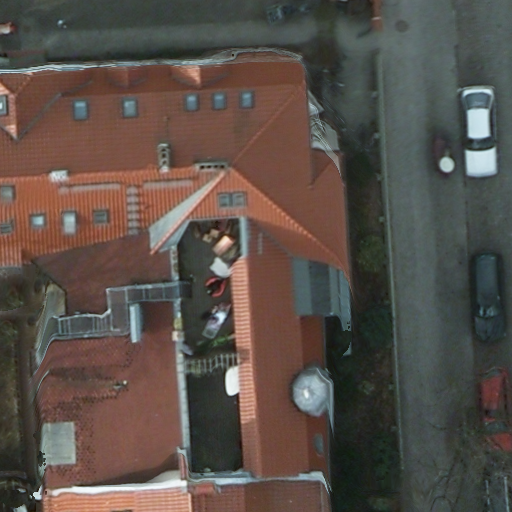
\includegraphics[width=3cm]{orthohr_rgb}};
\node[yshift=4pt] at (in_fig.north) {Image initiale};

\node (seg_fig) at (seg) {\includegraphics[width=3cm]{orthohr_rgb_slic}};
\node[yshift=-4pt] at (seg_fig.south) {Image segmentée};

\draw[ultra thick,->] ([xshift=0.8cm]in_fig.south) to node[left]{\small segmentation} ([xshift=0.8cm]seg_fig.north);

\node (large) at ($ (patches)+(0,2.5)$) {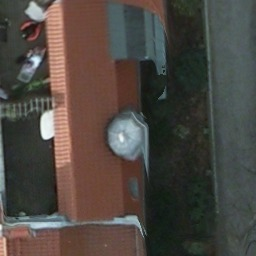
\includegraphics[width=2cm]{large}};
\node[yshift=-3pt] at (large.south) {contexte};
\node (medium) at (patches) {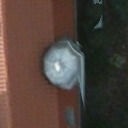
\includegraphics[width=2cm] {medium}};
\node[yshift=-3pt] at (medium.south) {contexte};
\node (ndsm) at ($ (patches)-(0,2.5) $) {\includegraphics[width=2cm]{ndsm}};
\node[yshift=-3pt] at (ndsm.south) {MNH};

\fill[line width=3pt,draw=red!95!black,fill=cyan!80!white,fill opacity=0.5,shading=axis, shading angle=135] (seg_fig.east) ++(-1.6,-1.1) --  +(0.6,0) -- +(0.6,0.6) -- +(0,0.6) -- cycle;

\draw (seg_fig.east) edge[in=180,out=0,->] (medium.west);
\draw (seg_fig.east) edge[in=180,out=0,->,looseness=0.8] (large.west);
\draw (seg_fig.east) edge[in=180,out=0,->] (ndsm.west);

\node[align=center] at ($ (patches)-(0,4.5) $) {Entrées multi-sources\\ et multi-échelles};

\node (net_fig) at (net) {\includegraphics[width=8cm]{../alexnet}};
\node at ($ (net) - (0,2)$) {CNN pré-entraîné};

\draw (large.east) edge[in=180,out=0,->] ([yshift=8pt]net_fig.west);
\draw (medium.east) edge[in=180,out=0,->] (net_fig.west);
\draw (ndsm.east) edge[in=180,out=0,->] ([yshift=-8pt]net_fig.west);

\coordinate (A) at ($ (features)+(0,-3,-0.5)$);
\coordinate (B) at ($ (features)+(0,3,-0.5)$);
\coordinate (C) at ($ (features)+(0.5,3,-0.5)$);
\coordinate (D) at ($ (features)+(0.5,-3,-0.5)$);
\coordinate (E) at ($ (features)+(0,-3,0)$);
\coordinate (F) at ($ (features)+(0,3,0)$);
\coordinate (G) at ($ (features)+(0.5,3,0)$);
\coordinate (H) at ($ (features)+(0.5,-3,0)$);

\coordinate (I) at ($ (E)!0.33!(F)$);
\coordinate (J) at ($ (E)!0.66!(F)$);
\coordinate (K) at ($ (H)!0.33!(G)$);
\coordinate (L) at ($ (H)!0.66!(G)$);
\coordinate (M) at ($ (D)!0.33!(C)$);
\coordinate (N) at ($ (D)!0.66!(C)$);

\def\grey{gray!40!white}
\draw[fill=\grey] (A) -- (B) -- (C) -- (D) -- cycle;
\draw[fill=\grey!60!white] (E) -- (F) -- (G) -- (H) -- cycle;
\draw[fill=\grey] (B) -- (C) -- (G) -- (F) -- cycle;
\draw[fill=\grey] (C) -- (D) -- (H) -- (G) -- cycle;
\draw[dotted,thick] (I) -- (K) -- (M);
\draw[dotted,thick] (J) -- (L) -- (N);
\node[align=center] at ($ (features) - (0,4.5)$) {Caractéristiques\\ profondes};

\draw ([yshift=-8pt]net_fig.east) edge[out=0,in=180,->] ($(I)!0.5!(E)$);
\draw ([yshift=8pt]net_fig.east) edge[out=0,in=180,->] ($(J)!0.5!(F)$);
\draw (net_fig.east) edge[out=0,in=180,->] ($(F)!0.5!(E)$);

\coordinate (c_A) at ($ (classifier) + (-1,1.5)$);
\coordinate (c_B) at ($ (classifier) + (-1,-1.5)$);
\coordinate (c_C) at ($ (classifier) + (1,-1.5)$);
\coordinate (c_D) at ($ (classifier) + (1,1.5)$);
\coordinate (c_top) at ($(c_A)!0.5!(c_D)$);
\coordinate (c_bottom) at ($ (c_B)!0.5!(c_C)$);
\filldraw[fill=yellow!50!white] (c_A) rectangle (c_C);


\newcommand\children[3]{
\coordinate (#1_c1) at ($(#1)!0.5!(#2)$);
\filldraw[fill=black] (#1_c1) circle (0.08);
\draw (#1) -- (#1_c1);
\coordinate (#1_c2) at ($(#1)!0.5!(#3)$);
\filldraw[fill=black] (#1_c2) circle (0.08);
\draw (#1) -- (#1_c2);
}

\coordinate (c_center) at ($(c_A)!0.5!(c_C)$);
\coordinate (c_center) at ($(c_center)!0.75!(c_top)$);
\filldraw[fill=black] (c_center) circle (0.1);
\coordinate (n1) at ($(c_center)!0.25!(c_B)$);
\filldraw[fill=black] (n1) circle (0.08);
\draw (c_center) -- (n1);
\coordinate (n2) at ($(c_center)!0.25!(c_C)$);
\filldraw[fill=black] (n2) circle (0.08);
\draw (c_center) -- (n2);

\children{n2}{c_bottom}{c_C}
\children{n2_c2}{c_bottom}{c_C}

\children{n1}{c_B}{c_bottom}
\children{n1_c1}{c_B}{c_bottom}

\node at ($(classifier) - (0,2)$) {Classifieur};

\draw ($(G)!0.5!(H)$) edge[ultra thick,in=180,out=0,->]  ($(c_A)!0.5!(c_B)$);

\node (map_fig) at (map) {\includegraphics[width=3cm]{gt_boundaries}};
\node[yshift=-4pt] at (map_fig.south) {Carte sémantique};
\fill[line width=3pt,draw=red!95!black,fill=cyan!50!white,fill opacity=0.2] (map_fig.east) ++(-1.6,-1.1) --  +(0.6,0) -- +(0.6,0.6) -- +(0,0.6) -- cycle;

\draw ($(c_C)!0.5!(c_D)$) edge[ultra thick,in=180,out=0,->] node[yshift=4pt,above]{Prédiction} node[yshift=-4pt,below]{\color{blue} ``Bâtiment''} (map_fig.west);

\end{tikzpicture}

\end{document}

}
\caption{Segmentation sémantique par régions d'une image aérienne. Chaque région de l'image segmentée est classifiée à partir de caractéristiques profondes extraites d'un réseau convolutif pré-entraîné.}
\label{fig:framework}
\end{figure}

Néanmoins, le nombre de pixels croissant quadratiquement avec la taille de l'image, ces approches passent difficilement à l'échelle, notamment en imagerie \gls{HR}, \gls{THR} et \gls{EHR}. Il est en effet inenvisageable de calculer une prédiction par pixel sur des images en comportant plusieurs millions, voire plusieurs milliards. L'alternative consiste à diminuer le nombre de passes d'inférence nécessaires en réalisant non pas une prédiction pour un unique pixel, mais pour une région toute entière.

L'approche de classification par régions consiste ainsi à regrouper ensemble des pixels similaires en régions homogènes. Le critère de similarité utilisé pour fusionner les pixels dépend à la fois de leurs valeurs et de leur position. Le classifieur réalise ensuite une inférence unique pour l'ensemble des pixels d'une même région, en faisant l'hypothèse que des pixels spatialement et spectralement proches possèdent la même sémantique, c'est-à-dire que l'on puisse les associer à la même classe d'intérêt. Dans ce cas, il suffit alors d'extraire des caractéristiques pour chaque région. Ainsi, dans le cas d'une image de dimensions $1 500\times1 500$ segmentée en \nombre{20000} régions, il devient possible de cartographier l'image en classifiant \nombre{20000} régions plutôt que \nombre{2250000} pixels.

De nombreux algorithmes de segmentation ont été proposés, aussi bien dans la communauté de la télédétection que dans la communauté de la vision par ordinateur. Ces algorithmes partitionnent l'ensemble des pixels de façon non-supervisée. Une fois ce partitionnement effectué, il est possible d'extraire des attributs pour chaque région et d'entraîner un classifieur de la façon habituelle, comme détaillé dans la~\cref{fig:framework}.

Réaliser une classification par régions permet de significativement réduire la complexité calculatoire de la cartographie. Lorsque l'image augmente de résolution spatiale, la plupart des régions conservent leur homogénéité et il est ainsi avantageux de les conserver regroupées\,: l'augmentation de la résolution n'implique pas obligatoirement une évolution quadratique du nombre de régions. Depuis les premiers travaux de~\citet{mnih_machine_2013} utilisant les \glspl{CNN} pour l'extraction de routes et de bâtiments dans des images aériennes à partir d'imagettes, ces approches ont ainsi été utilisées avec succès sur de nombreux jeux de données \gls{THR}~\cite{lagrange_benchmarking_2015,vargas_superpixel-based_2014}. Notons par ailleurs que traiter l'image par une fenêtre glissante ou même par une grille de pixels correspond à des cas particuliers de classification par région.

Dans les cas des profils morphologiques, ces approches par pré-segmentation sont d'autant plus intéressantes que les opérateurs morphologiques sont coûteux à calculer. Une alternative classique est d'opérer sur une segmentation multi-échelle hiérarchique de l'image, représentée sous forme d'arbre. Les opérations de filtrage morphologique se traduisent en opérations d'élagage de l'arbre, rapides à calculer. De nombreuses approches de construction d'arbres existent~\cite{bosilj_indexation_2016}, permettant de construire des profils d'attributs, c'est-à-dire des caractéristiques multi-échelles étendant les propriétés des profils morphologiques. Ces approches ont longtemps représenté l'état de l'art en cartographie automatisée~\cite{pham_feature_2018} et des modèles statistiques spécifiques ont été développés pour en tirer parti~\cite{cui_combining_2016}.

En parallèle de cette thèse, les approches utilisant les \glslink{FCN}{réseaux entièrement convolutifs (FCN)} pour la segmentation sémantique d'images de télédétection se sont nettement popularisées. En effet, les \gls{FCN} infèrent une prédiction pixellique pour l'ensemble de l'image en une seule passe, s'affranchissant ainsi du problème de la classification par \emph{patch}. Cela réduit drastiquement les temps de calcul, sans pour autant nécessiter une pré-segmentation non supervisée. Les premières applications de \gls{FCN} sur des données aériennes optiques apparaissent en 2015 chez \citet{paisitkriangkrai_effective_2015,sherrah_fully_2016} en se basant sur les architectures initiales de~\citet{long_fully_2015}. Les modèles encodeur-décodeurs symétriques suivent rapidement~\cite{volpi_dense_2017,audebert_semantic_2016} et sont le sujet de plusieurs travaux dérivés, comme la conception d'un~\gls{CRF}~\cite{liu_dense_2017} pour la fusion de données ou la régularisation des bordures par contrainte explicite~\cite{marmanis_classification_2017}. Si les images aériennes \gls{EHR} sont naturellement les premières candidates, les \gls{FCN} sont également mis en \oe{}uvre pour la cartographie d'images satellites~\cite{fu_classification_2017}.

De nouveaux jeux de données comme l'\emph{Inria Aerial Image Labeling Dataset} fournissent un terrain de jeu propice aux réseaux entièrement convolutifs, qui dominent très largement les classements~\cite{huang_large-scale_2018}. Dans l'ensemble, les méthodes par apprentissage profond utilisant les \gls{FCN} se sont imposées en quelques années comme le nouvel état de l'art sur de nombreuses tâches d'interprétation d'images de télédétection~\cite{liu_comparing_2018}. L'apparition de nombreux jeux de données annotés de télédétection, détaillés en~\cref{chap:datasets}, a notamment permis d'entraîner des modèles profonds sur une large gamme d'applications.

%\bibliographystyle{plainnat}
%\bibliography{Chapitre1/Historique}
\printbibliography
